% Options for packages loaded elsewhere
\PassOptionsToPackage{unicode}{hyperref}
\PassOptionsToPackage{hyphens}{url}
\PassOptionsToPackage{dvipsnames,svgnames,x11names}{xcolor}
%
\documentclass[
  letterpaper,
  DIV=11,
  numbers=noendperiod]{scrreprt}

\usepackage{amsmath,amssymb}
\usepackage{iftex}
\ifPDFTeX
  \usepackage[T1]{fontenc}
  \usepackage[utf8]{inputenc}
  \usepackage{textcomp} % provide euro and other symbols
\else % if luatex or xetex
  \usepackage{unicode-math}
  \defaultfontfeatures{Scale=MatchLowercase}
  \defaultfontfeatures[\rmfamily]{Ligatures=TeX,Scale=1}
\fi
\usepackage{lmodern}
\ifPDFTeX\else  
    % xetex/luatex font selection
\fi
% Use upquote if available, for straight quotes in verbatim environments
\IfFileExists{upquote.sty}{\usepackage{upquote}}{}
\IfFileExists{microtype.sty}{% use microtype if available
  \usepackage[]{microtype}
  \UseMicrotypeSet[protrusion]{basicmath} % disable protrusion for tt fonts
}{}
\makeatletter
\@ifundefined{KOMAClassName}{% if non-KOMA class
  \IfFileExists{parskip.sty}{%
    \usepackage{parskip}
  }{% else
    \setlength{\parindent}{0pt}
    \setlength{\parskip}{6pt plus 2pt minus 1pt}}
}{% if KOMA class
  \KOMAoptions{parskip=half}}
\makeatother
\usepackage{xcolor}
\ifLuaTeX
  \usepackage{luacolor}
  \usepackage[soul]{lua-ul}
\else
  \usepackage{soul}
  
\fi
\setlength{\emergencystretch}{3em} % prevent overfull lines
\setcounter{secnumdepth}{5}
% Make \paragraph and \subparagraph free-standing
\ifx\paragraph\undefined\else
  \let\oldparagraph\paragraph
  \renewcommand{\paragraph}[1]{\oldparagraph{#1}\mbox{}}
\fi
\ifx\subparagraph\undefined\else
  \let\oldsubparagraph\subparagraph
  \renewcommand{\subparagraph}[1]{\oldsubparagraph{#1}\mbox{}}
\fi

\usepackage{color}
\usepackage{fancyvrb}
\newcommand{\VerbBar}{|}
\newcommand{\VERB}{\Verb[commandchars=\\\{\}]}
\DefineVerbatimEnvironment{Highlighting}{Verbatim}{commandchars=\\\{\}}
% Add ',fontsize=\small' for more characters per line
\usepackage{framed}
\definecolor{shadecolor}{RGB}{241,243,245}
\newenvironment{Shaded}{\begin{snugshade}}{\end{snugshade}}
\newcommand{\AlertTok}[1]{\textcolor[rgb]{0.68,0.00,0.00}{#1}}
\newcommand{\AnnotationTok}[1]{\textcolor[rgb]{0.37,0.37,0.37}{#1}}
\newcommand{\AttributeTok}[1]{\textcolor[rgb]{0.40,0.45,0.13}{#1}}
\newcommand{\BaseNTok}[1]{\textcolor[rgb]{0.68,0.00,0.00}{#1}}
\newcommand{\BuiltInTok}[1]{\textcolor[rgb]{0.00,0.23,0.31}{#1}}
\newcommand{\CharTok}[1]{\textcolor[rgb]{0.13,0.47,0.30}{#1}}
\newcommand{\CommentTok}[1]{\textcolor[rgb]{0.37,0.37,0.37}{#1}}
\newcommand{\CommentVarTok}[1]{\textcolor[rgb]{0.37,0.37,0.37}{\textit{#1}}}
\newcommand{\ConstantTok}[1]{\textcolor[rgb]{0.56,0.35,0.01}{#1}}
\newcommand{\ControlFlowTok}[1]{\textcolor[rgb]{0.00,0.23,0.31}{#1}}
\newcommand{\DataTypeTok}[1]{\textcolor[rgb]{0.68,0.00,0.00}{#1}}
\newcommand{\DecValTok}[1]{\textcolor[rgb]{0.68,0.00,0.00}{#1}}
\newcommand{\DocumentationTok}[1]{\textcolor[rgb]{0.37,0.37,0.37}{\textit{#1}}}
\newcommand{\ErrorTok}[1]{\textcolor[rgb]{0.68,0.00,0.00}{#1}}
\newcommand{\ExtensionTok}[1]{\textcolor[rgb]{0.00,0.23,0.31}{#1}}
\newcommand{\FloatTok}[1]{\textcolor[rgb]{0.68,0.00,0.00}{#1}}
\newcommand{\FunctionTok}[1]{\textcolor[rgb]{0.28,0.35,0.67}{#1}}
\newcommand{\ImportTok}[1]{\textcolor[rgb]{0.00,0.46,0.62}{#1}}
\newcommand{\InformationTok}[1]{\textcolor[rgb]{0.37,0.37,0.37}{#1}}
\newcommand{\KeywordTok}[1]{\textcolor[rgb]{0.00,0.23,0.31}{#1}}
\newcommand{\NormalTok}[1]{\textcolor[rgb]{0.00,0.23,0.31}{#1}}
\newcommand{\OperatorTok}[1]{\textcolor[rgb]{0.37,0.37,0.37}{#1}}
\newcommand{\OtherTok}[1]{\textcolor[rgb]{0.00,0.23,0.31}{#1}}
\newcommand{\PreprocessorTok}[1]{\textcolor[rgb]{0.68,0.00,0.00}{#1}}
\newcommand{\RegionMarkerTok}[1]{\textcolor[rgb]{0.00,0.23,0.31}{#1}}
\newcommand{\SpecialCharTok}[1]{\textcolor[rgb]{0.37,0.37,0.37}{#1}}
\newcommand{\SpecialStringTok}[1]{\textcolor[rgb]{0.13,0.47,0.30}{#1}}
\newcommand{\StringTok}[1]{\textcolor[rgb]{0.13,0.47,0.30}{#1}}
\newcommand{\VariableTok}[1]{\textcolor[rgb]{0.07,0.07,0.07}{#1}}
\newcommand{\VerbatimStringTok}[1]{\textcolor[rgb]{0.13,0.47,0.30}{#1}}
\newcommand{\WarningTok}[1]{\textcolor[rgb]{0.37,0.37,0.37}{\textit{#1}}}

\providecommand{\tightlist}{%
  \setlength{\itemsep}{0pt}\setlength{\parskip}{0pt}}\usepackage{longtable,booktabs,array}
\usepackage{calc} % for calculating minipage widths
% Correct order of tables after \paragraph or \subparagraph
\usepackage{etoolbox}
\makeatletter
\patchcmd\longtable{\par}{\if@noskipsec\mbox{}\fi\par}{}{}
\makeatother
% Allow footnotes in longtable head/foot
\IfFileExists{footnotehyper.sty}{\usepackage{footnotehyper}}{\usepackage{footnote}}
\makesavenoteenv{longtable}
\usepackage{graphicx}
\makeatletter
\def\maxwidth{\ifdim\Gin@nat@width>\linewidth\linewidth\else\Gin@nat@width\fi}
\def\maxheight{\ifdim\Gin@nat@height>\textheight\textheight\else\Gin@nat@height\fi}
\makeatother
% Scale images if necessary, so that they will not overflow the page
% margins by default, and it is still possible to overwrite the defaults
% using explicit options in \includegraphics[width, height, ...]{}
\setkeys{Gin}{width=\maxwidth,height=\maxheight,keepaspectratio}
% Set default figure placement to htbp
\makeatletter
\def\fps@figure{htbp}
\makeatother
% definitions for citeproc citations
\NewDocumentCommand\citeproctext{}{}
\NewDocumentCommand\citeproc{mm}{%
  \begingroup\def\citeproctext{#2}\cite{#1}\endgroup}
\makeatletter
 % allow citations to break across lines
 \let\@cite@ofmt\@firstofone
 % avoid brackets around text for \cite:
 \def\@biblabel#1{}
 \def\@cite#1#2{{#1\if@tempswa , #2\fi}}
\makeatother
\newlength{\cslhangindent}
\setlength{\cslhangindent}{1.5em}
\newlength{\csllabelwidth}
\setlength{\csllabelwidth}{3em}
\newenvironment{CSLReferences}[2] % #1 hanging-indent, #2 entry-spacing
 {\begin{list}{}{%
  \setlength{\itemindent}{0pt}
  \setlength{\leftmargin}{0pt}
  \setlength{\parsep}{0pt}
  % turn on hanging indent if param 1 is 1
  \ifodd #1
   \setlength{\leftmargin}{\cslhangindent}
   \setlength{\itemindent}{-1\cslhangindent}
  \fi
  % set entry spacing
  \setlength{\itemsep}{#2\baselineskip}}}
 {\end{list}}
\usepackage{calc}
\newcommand{\CSLBlock}[1]{\hfill\break\parbox[t]{\linewidth}{\strut\ignorespaces#1\strut}}
\newcommand{\CSLLeftMargin}[1]{\parbox[t]{\csllabelwidth}{\strut#1\strut}}
\newcommand{\CSLRightInline}[1]{\parbox[t]{\linewidth - \csllabelwidth}{\strut#1\strut}}
\newcommand{\CSLIndent}[1]{\hspace{\cslhangindent}#1}

\KOMAoption{captions}{tableheading}
\makeatletter
\@ifpackageloaded{tcolorbox}{}{\usepackage[skins,breakable]{tcolorbox}}
\@ifpackageloaded{fontawesome5}{}{\usepackage{fontawesome5}}
\definecolor{quarto-callout-color}{HTML}{909090}
\definecolor{quarto-callout-note-color}{HTML}{0758E5}
\definecolor{quarto-callout-important-color}{HTML}{CC1914}
\definecolor{quarto-callout-warning-color}{HTML}{EB9113}
\definecolor{quarto-callout-tip-color}{HTML}{00A047}
\definecolor{quarto-callout-caution-color}{HTML}{FC5300}
\definecolor{quarto-callout-color-frame}{HTML}{acacac}
\definecolor{quarto-callout-note-color-frame}{HTML}{4582ec}
\definecolor{quarto-callout-important-color-frame}{HTML}{d9534f}
\definecolor{quarto-callout-warning-color-frame}{HTML}{f0ad4e}
\definecolor{quarto-callout-tip-color-frame}{HTML}{02b875}
\definecolor{quarto-callout-caution-color-frame}{HTML}{fd7e14}
\makeatother
\makeatletter
\@ifpackageloaded{bookmark}{}{\usepackage{bookmark}}
\makeatother
\makeatletter
\@ifpackageloaded{caption}{}{\usepackage{caption}}
\AtBeginDocument{%
\ifdefined\contentsname
  \renewcommand*\contentsname{Table of contents}
\else
  \newcommand\contentsname{Table of contents}
\fi
\ifdefined\listfigurename
  \renewcommand*\listfigurename{List of Figures}
\else
  \newcommand\listfigurename{List of Figures}
\fi
\ifdefined\listtablename
  \renewcommand*\listtablename{List of Tables}
\else
  \newcommand\listtablename{List of Tables}
\fi
\ifdefined\figurename
  \renewcommand*\figurename{Figure}
\else
  \newcommand\figurename{Figure}
\fi
\ifdefined\tablename
  \renewcommand*\tablename{Table}
\else
  \newcommand\tablename{Table}
\fi
}
\@ifpackageloaded{float}{}{\usepackage{float}}
\floatstyle{ruled}
\@ifundefined{c@chapter}{\newfloat{codelisting}{h}{lop}}{\newfloat{codelisting}{h}{lop}[chapter]}
\floatname{codelisting}{Listing}
\newcommand*\listoflistings{\listof{codelisting}{List of Listings}}
\makeatother
\makeatletter
\makeatother
\makeatletter
\@ifpackageloaded{caption}{}{\usepackage{caption}}
\@ifpackageloaded{subcaption}{}{\usepackage{subcaption}}
\makeatother
\ifLuaTeX
  \usepackage{selnolig}  % disable illegal ligatures
\fi
\usepackage{bookmark}

\IfFileExists{xurl.sty}{\usepackage{xurl}}{} % add URL line breaks if available
\urlstyle{same} % disable monospaced font for URLs
\hypersetup{
  pdftitle={R 4 Epidemiology},
  colorlinks=true,
  linkcolor={blue},
  filecolor={Maroon},
  citecolor={Blue},
  urlcolor={Blue},
  pdfcreator={LaTeX via pandoc}}

\title{R 4 Epidemiology}
\author{}
\date{2024-07-29}

\begin{document}
\maketitle

\renewcommand*\contentsname{Table of contents}
{
\hypersetup{linkcolor=}
\setcounter{tocdepth}{2}
\tableofcontents
}
\bookmarksetup{startatroot}

\chapter*{Welcome}\label{welcome}
\addcontentsline{toc}{chapter}{Welcome}

\markboth{Welcome}{Welcome}

Welcome to R for Epidemiology!

This electronic textbook was originally created to accompany the
Introduction to R Programming for Epidemiologic Research course at the
\href{https://sph.uth.edu/}{University of Texas Health Science Center
School of Public Health}. However, we hope it will be useful to anyone
who is interested in R, epidemiology, or human health and well-being.

\section*{Acknowledgements}\label{acknowledgements}
\addcontentsline{toc}{section}{Acknowledgements}

\markright{Acknowledgements}

This book is currently a work in progress (and probably always will be);
however, there are already many people who have played an important role
(some unknowingly) in helping develop it thus far. First, we'd like to
offer our gratitude to all past, current, and future members of the R
Core Team for maintaining this \emph{amazing}, \emph{free} software.
We'd also like to express our gratitude to everyone at
\href{https://posit.co/}{Posit}. You are also developing and
\emph{giving away} some amazing software. In particular, we'd like to
acknowledge
\href{https://www.linkedin.com/in/garrett-grolemund-49328411/}{Garrett
Grolemund} and \href{https://hadley.nz/}{Hadley Wickham}. Both have had
a huge impact on how we use and teach R. We'd also like to thank our
students for all the feedback they've given us while taking our courses.
In particular, we want to thank
\href{https://www.linkedin.com/in/jared-wiegand/}{Jared Wiegand} and
Yiqun Wang for their many edits and suggestions.

This electronic textbook was created and published using
\href{https://cran.r-project.org/}{R},
\href{https://www.rstudio.com/}{RStudio}, the
\href{https://quarto.org/}{Quarto}, and
\href{https://github.com/}{GitHub}.

\bookmarksetup{startatroot}

\chapter*{Introduction}\label{introduction}
\addcontentsline{toc}{chapter}{Introduction}

\markboth{Introduction}{Introduction}

\section*{Goals}\label{goals}
\addcontentsline{toc}{section}{Goals}

\markright{Goals}

We're going to start the introduction by writing down some basic goals
that underlie the construction and content of this book. We're writing
this for you, the reader, but also to hold ourselves accountable as we
write. So, feel free to read if you are interested or skip ahead if you
aren't.

The goals of this book are:

\begin{enumerate}
\def\labelenumi{\arabic{enumi}.}
\item
  \textbf{To teach you how to use R and RStudio as tools for applied
  epidemiology}.\footnote{In this case, ``tools for applied
    epidemiology'' means (1) understanding epidemiologic concepts; and
    (2) completing and interpreting epidemiologic analyses.} Our goal is
  not to teach you to be a computer scientist or an advanced R
  programmer. Therefore, some readers who are experienced programmers
  may catch some technical inaccuracies regarding what we consider to be
  the fine points of what R is doing ``under the hood.''
\item
  \textbf{To make this writing as accessible and practically useful as
  possible without stripping out all of the complexity that makes doing
  epidemiology in real life a challenge}. In other words, We're going to
  try to give you all the tools you need to \emph{do} epidemiology in
  ``real world'' conditions (as opposed to ideal conditions) without
  providing a whole bunch of extraneous (often theoretical) stuff that
  detracts from \emph{doing}. Having said that, we will strive to add
  links to the other (often theoretical) stuff for readers who are
  interested.
\item
  \textbf{To teach you to accomplish common \emph{tasks}}, rather than
  teach you to use functions or families of functions. In many R courses
  and texts, there is a focus on learning all the things a function, or
  set of related functions, can do. It's then up to you, the reader, to
  sift through all of these capabilities and decided which, if any, of
  the things that \emph{can} be done will accomplish the tasks that you
  are \emph{actually trying} to accomplish. Instead, we will strive to
  start with the end in mind. What is the task we are actually trying to
  accomplish? What are some functions/methods we could use to accomplish
  that task? What are the strengths and limitations of each?
\item
  \textbf{To start each concept by showing you the end result} and then
  deconstruct how we arrived at that result, where possible. We find
  that it is easier for many people to understand new concepts when
  learning them as a component of a final product.
\item
  \textbf{To learn concepts with data} instead of (or alongside)
  mathematical formulas and text descriptions, where possible. We find
  that it is easier for many people to understand new concepts by seeing
  them in action.
\end{enumerate}

\section*{Text conventions used in this
book}\label{text-conventions-used-in-this-book}
\addcontentsline{toc}{section}{Text conventions used in this book}

\markright{Text conventions used in this book}

\begin{itemize}
\tightlist
\item
  We will hyperlink many keywords or phrases to their
  \href{appendices/glossary.qmd}{glossary} entry.
\item
  Additionally, we may use \textbf{bold} face for a word or phrase that
  we want to call attention to, but it is not necessarily a keyword or
  phrase that we want to define in the glossary.
\item
  \texttt{Highlighted\ inline\ code} is used to emphasize small sections
  of R code and program elements such as variable or function names.
\end{itemize}

\section*{Other reading}\label{other-reading}
\addcontentsline{toc}{section}{Other reading}

\markright{Other reading}

If you are interested in R4Epi, you may also be interested in:

\begin{itemize}
\item
  \href{https://rstudio-education.github.io/hopr/}{Hands-on Programming
  with R} by Garrett Grolemund. This book is designed to provide a
  friendly introduction to the R language.
\item
  \href{https://r4ds.hadley.nz/}{R for Data Science} by Hadley Wickham,
  Mine Çetinkaya-Rundel, and Garrett Grolemund. This book is designed to
  teach readers how to do data science with R.
\item
  \href{https://moderndive.com/}{Statistical Inference via Data Science:
  A ModernDive into R and the Tidyverse}. This book is designed to be a
  gentle introduction to the practice of analyzing data and answering
  questions using data the way data scientists, statisticians, data
  journalists, and other researchers would.
\item
  \href{http://christophergandrud.github.io/RepResR-RStudio/}{Reproducable
  Research with R and RStudio} by Christopher Gandrud. This book gives
  you tools for data gathering, analysis, and presentation of results so
  that you can create dynamic and highly reproducible research.
\item
  \href{https://adv-r.hadley.nz/}{Advanced R} by Hadley Wickham. This
  book is designed primarily for R users who want to improve their
  programming skills and understanding of the language.
\end{itemize}

\bookmarksetup{startatroot}

\chapter*{Contributing}\label{contributing}
\addcontentsline{toc}{chapter}{Contributing}

\markboth{Contributing}{Contributing}

Over the years, we have learned so much from our students and
colleagues, and we anticipate that there is much more we can learn from
you -- our readers. Therefore, we welcome and appreciate all
constructive contributions to R4Epi!

\section*{Typos}\label{typos}
\addcontentsline{toc}{section}{Typos}

\markright{Typos}

The easiest way for you to contribute is to help us clean up the little
typos and grammatical errors that inevitably sneak into the text.

If you spot a typo, you can offer a correction directly in GitHub. You
will first need to create a free GitHub account:
\href{https://github.com/join}{sign-up at github.com}. Later in the
book, we will cover using GitHub in greater depth (See
Chapter~\ref{sec-using-git-and-github}). Here, we're just going to walk
you through how to fix a typo without much explanation of how GitHub
works.

Let's say you spot a typo while reading along.

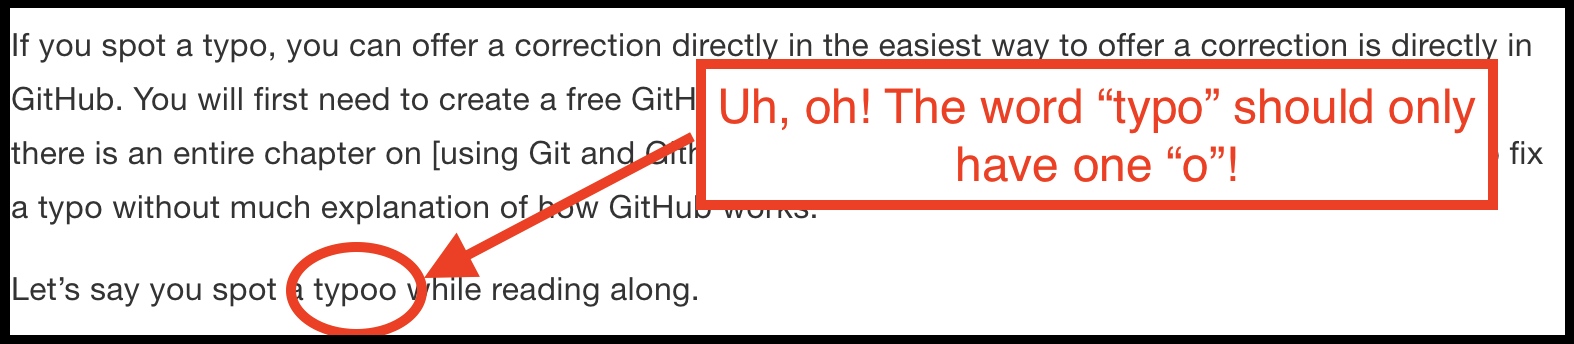
\includegraphics{chapters/contributing/typo_on_screen.png}

Next, click the edit button in the toolbar as shown in the screenshot
below.

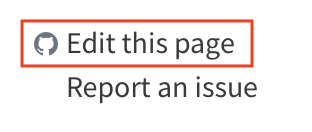
\includegraphics{chapters/contributing/edit_button.png}

The first time you click the icon, you will be taken to the R4Epi
repository on GitHub and asked to fork it. For our purposes, you can
think of a GitHub repository as being similar to a shared folder on
Dropbox or Google Drive.


\includegraphics{chapters/contributing/fork_button.png}

``Forking the repository'' basically just means ``make a copy of the
repository'' on your GitHub account. In other words, copy all of the
files that make up the R4Epi textbook to your GitHub account. Then, you
can fix the typos you found in your \emph{copy} of the files that make
up the book instead of directly editing the \emph{actual} files that
make up the book. This is a safeguard to prevent people from
accidentally making changes that shouldn't be made.

\begin{tcolorbox}[enhanced jigsaw, rightrule=.15mm, breakable, colback=white, bottomtitle=1mm, title=\textcolor{quarto-callout-note-color}{\faInfo}\hspace{0.5em}{Note}, colframe=quarto-callout-note-color-frame, opacityback=0, coltitle=black, colbacktitle=quarto-callout-note-color!10!white, opacitybacktitle=0.6, toptitle=1mm, bottomrule=.15mm, left=2mm, leftrule=.75mm, titlerule=0mm, toprule=.15mm, arc=.35mm]

Forking the R4Epi repository does not cost any money or add any files to
your computer.

\end{tcolorbox}

After you fork the repository, you will see a text editor on your
screen.

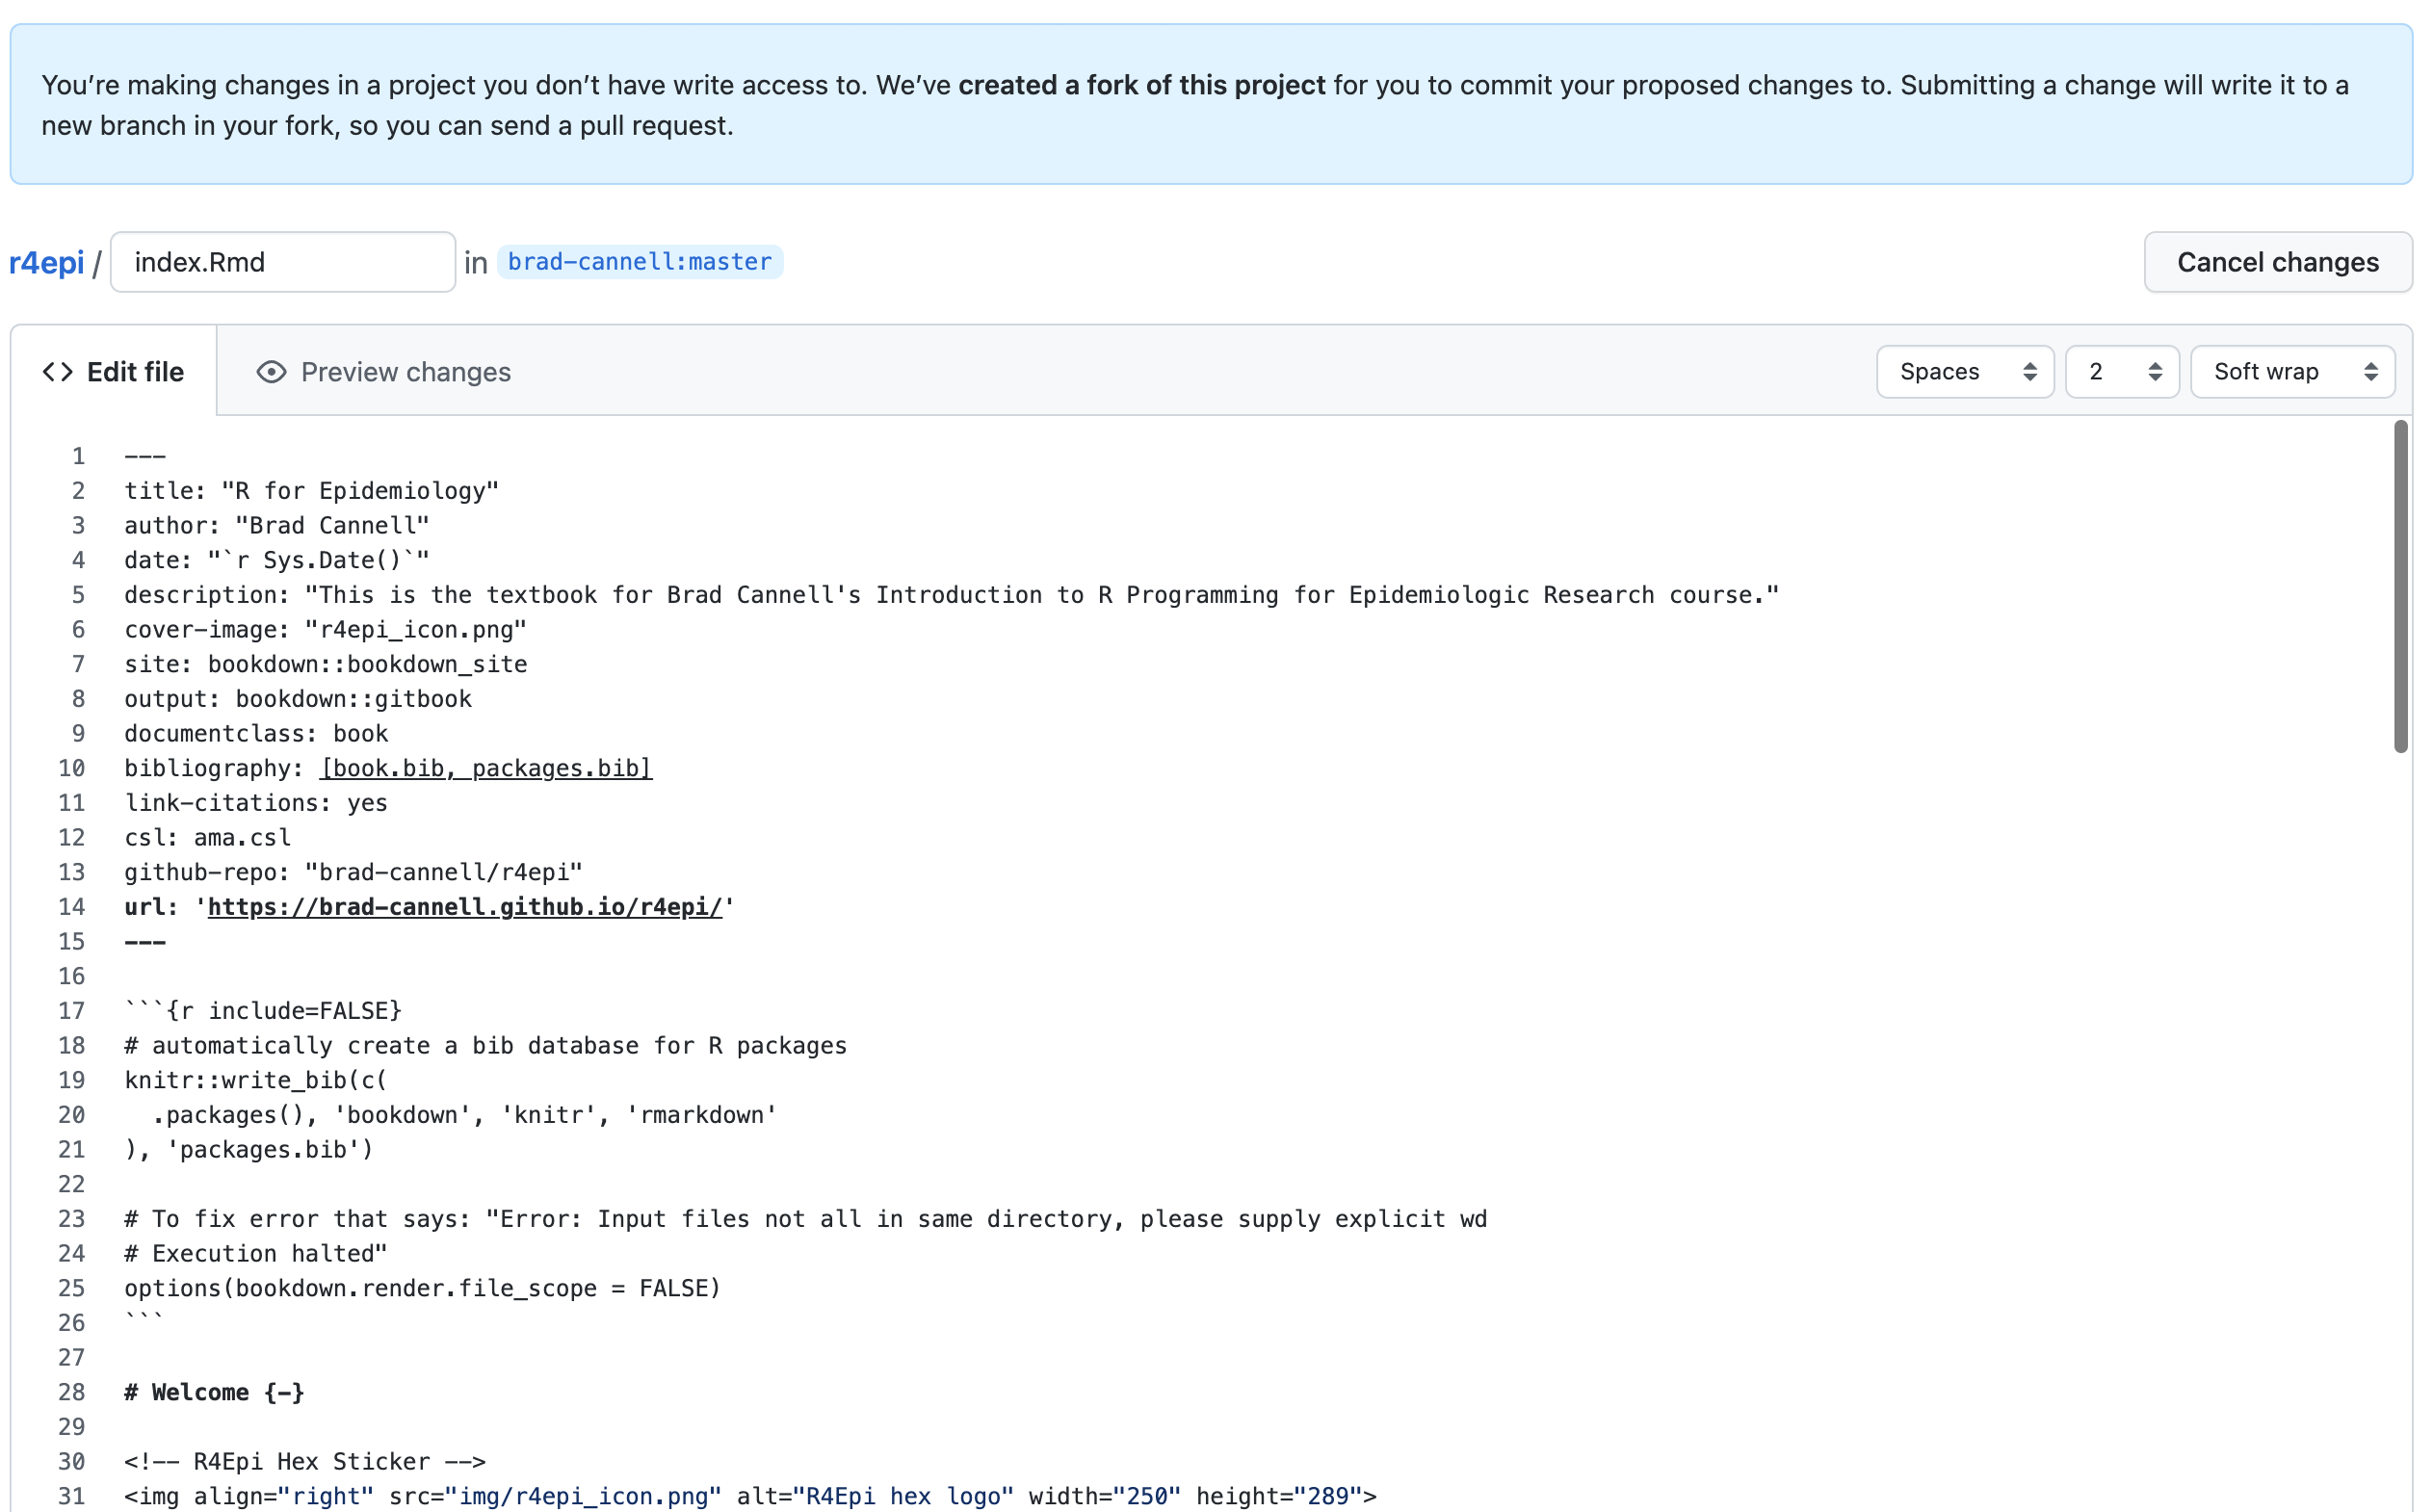
\includegraphics{chapters/contributing/text_editor.png}

The text editor will display the contents of the file used to make the
chapter you were looking at when you clicked the \texttt{edit} button.
In this example, it was a file named \texttt{contributing.qmd}. The
\texttt{.qmd} file extension means that the file is a Quarto file. We
will learn more about Quarto files in \textbf{?@sec-quarto-files}, but
for now just know that Quarto files can be used to create web pages and
other documents that contain a mix of R code, text, and images.

Next, scroll down through the text until you find the typo and fix it.
In this case, line 11 contains the word ``typoo''. To fix it, you just
need to click in the editor window and begin typing. In this case, you
would click next to the word ``typoo'' and delete the second ``o''.

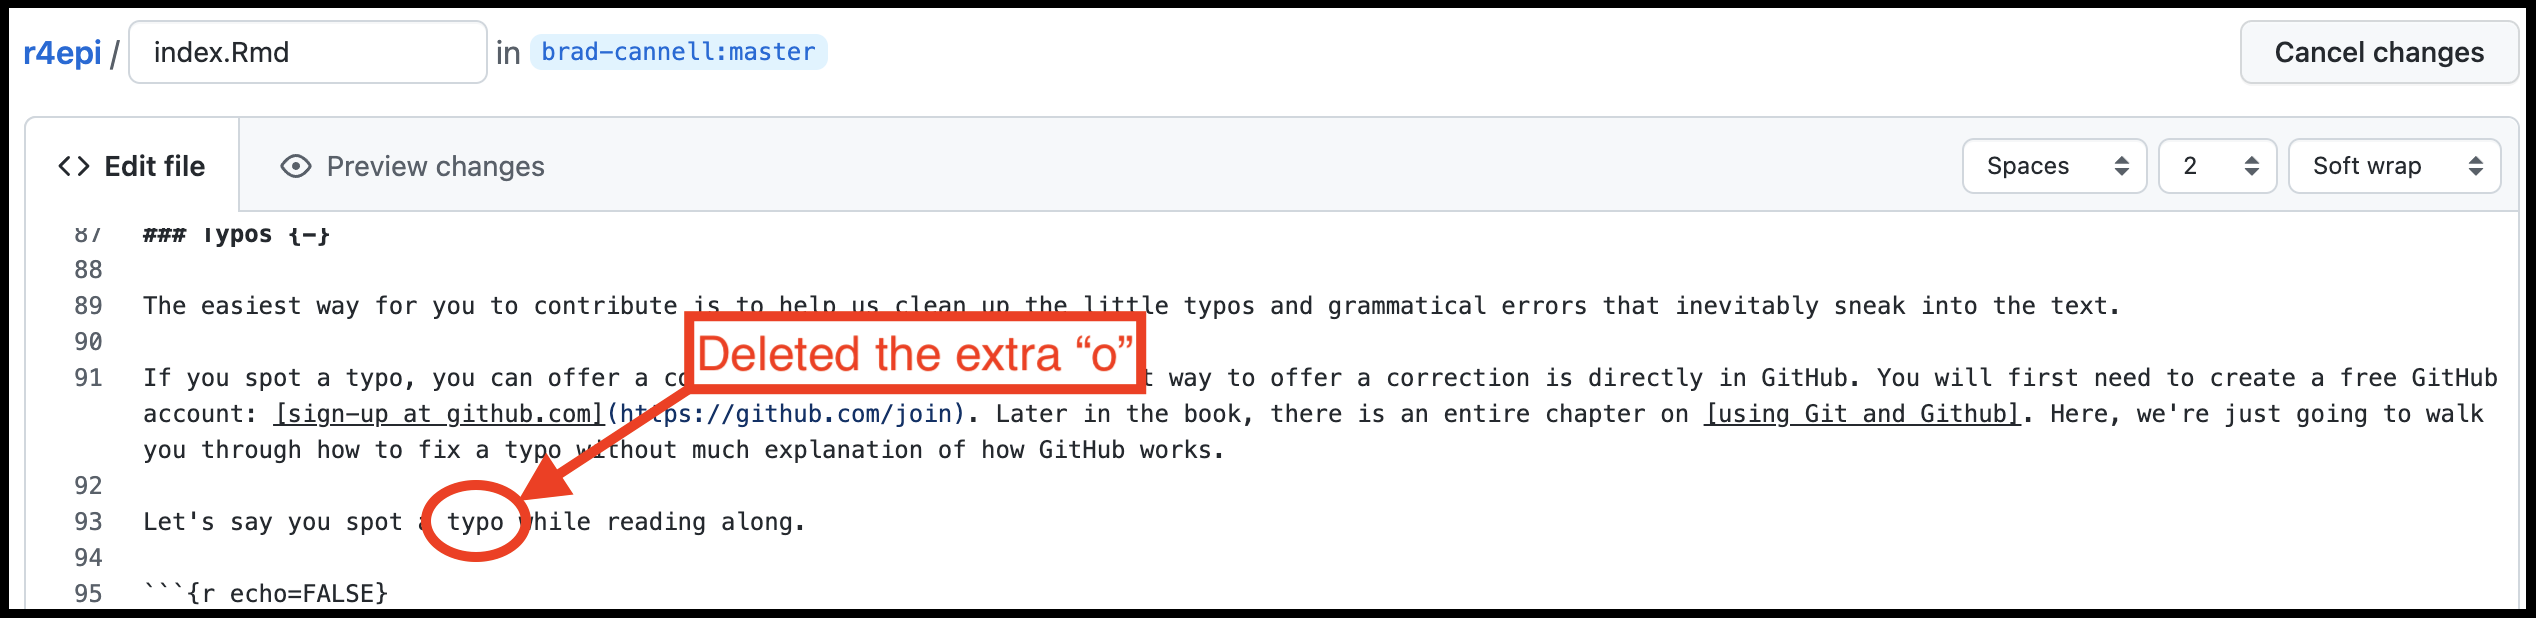
\includegraphics{chapters/contributing/fix_typo.png}

Now, the only thing left to do is propose your typo fix to the authors.
To do so, click the green \texttt{Commit\ changes...} button on the
right side of the screen above the text editor (surrounded with a red
box in the screenshot above). When you click it, a new
\texttt{Propose\ changes} box will appear on your screen. Type a brief
(i.e., 72 characters or less) summary of the change you made in the
\texttt{Commit\ message} box. There is also an
\texttt{Extended\ description} box where you can add a more detailed
description of what you did. In the screenshot below, shows an example
commit message and extended description that will make it easy for the
author to quickly figure out exactly what changes are being proposed.

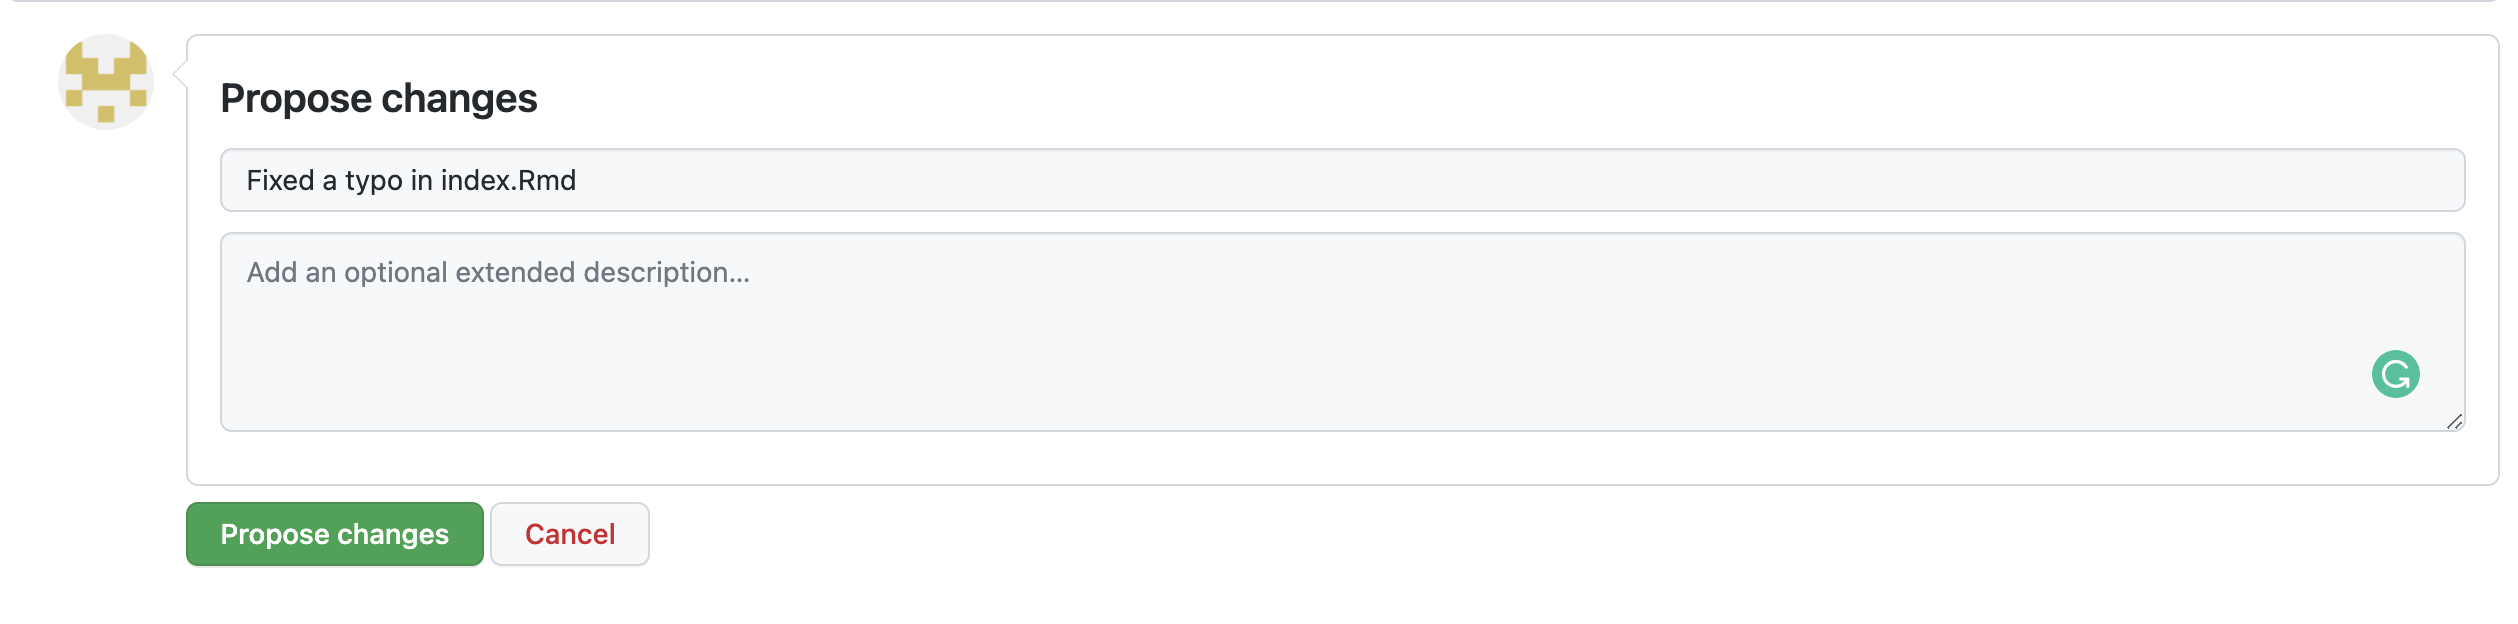
\includegraphics{chapters/contributing/propose_changes.png}

Next, click the \texttt{Propose\ changes} button. That will take you to
another screen where you will be able to create a pull request. This
screen is kind of busy, but try not to let it overwhelm you.

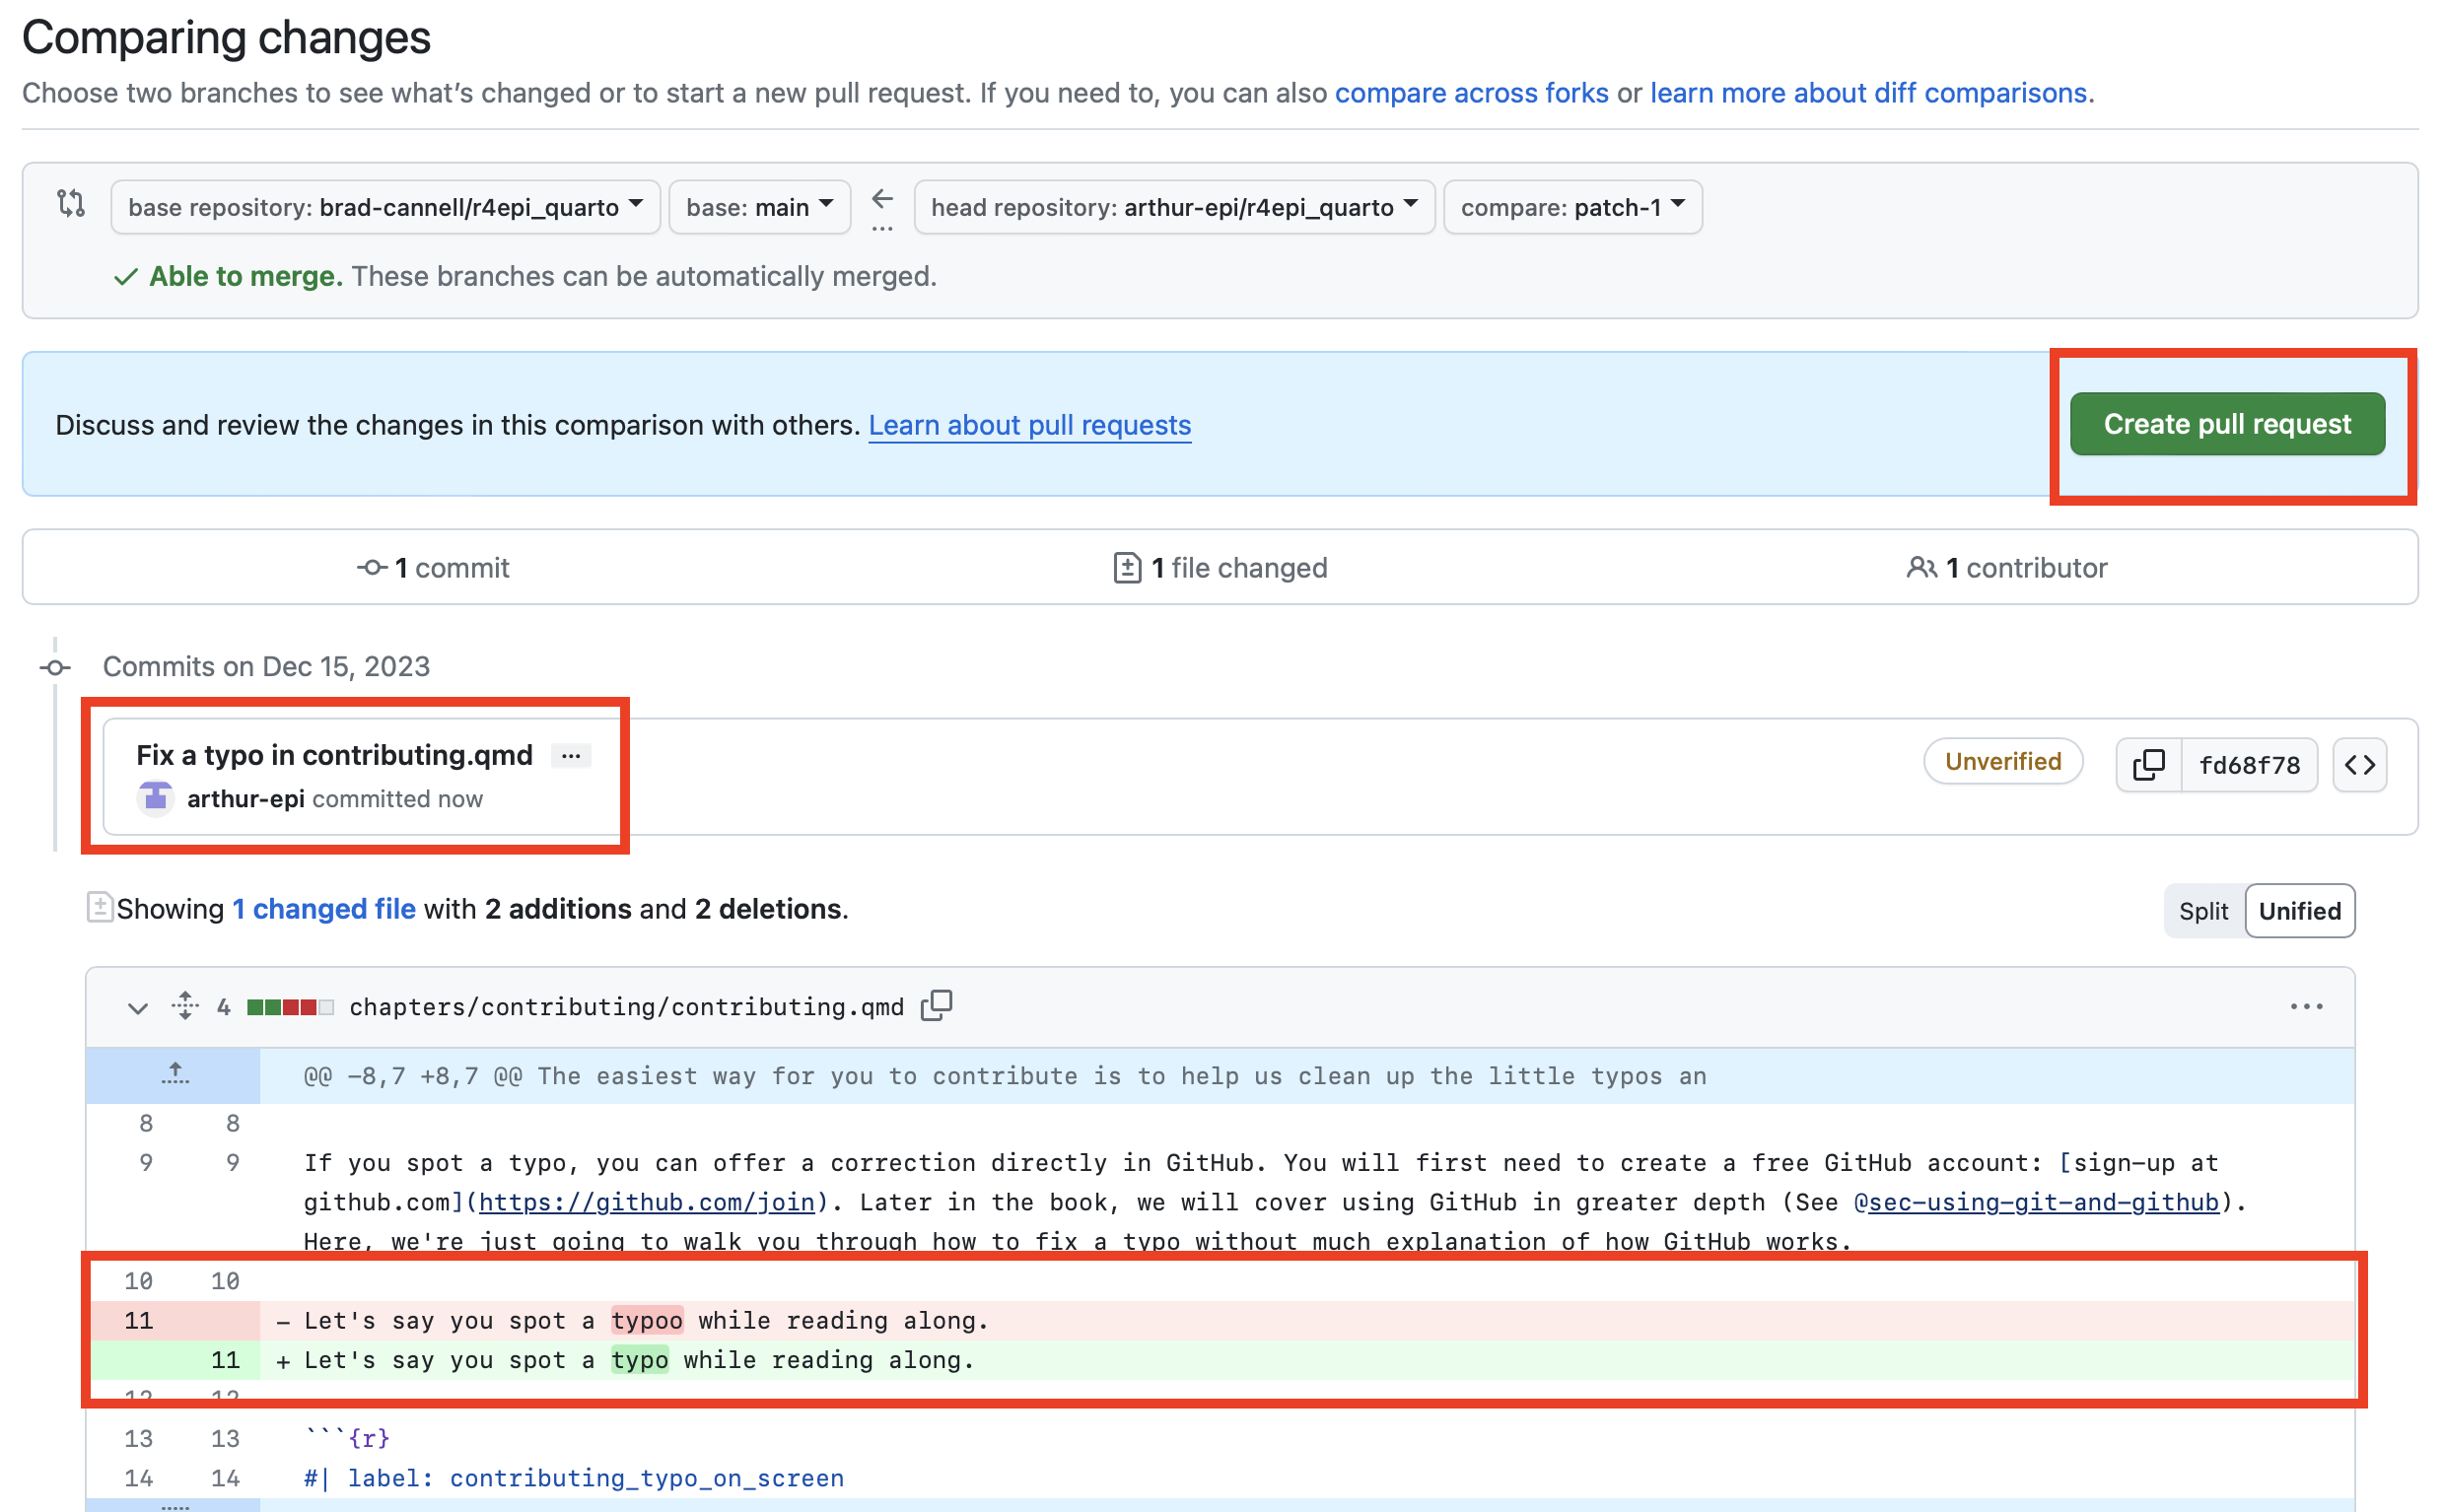
\includegraphics{chapters/contributing/create_pull_request_1.png}

For now, we will focus on the three different sections of the screen
that are highlighted with a red outline. We will start at the bottom and
work our way up. The red box that is closest to the bottom of the
screenshot shows us that the change that made was on line 11. The word
``typoo'' (highlighted in red) was replaced with the word ``typo''
(highlighted in green). The red box in the middle of the screenshot
shows us the brief description that was written for our proposed change
-- ``Fix a typo in contributing.qmd''. Finally, the red box closest to
the top of the screenshot is surrounding the
\texttt{Create\ pull\ request} button. You will click it to move on with
your pull request.

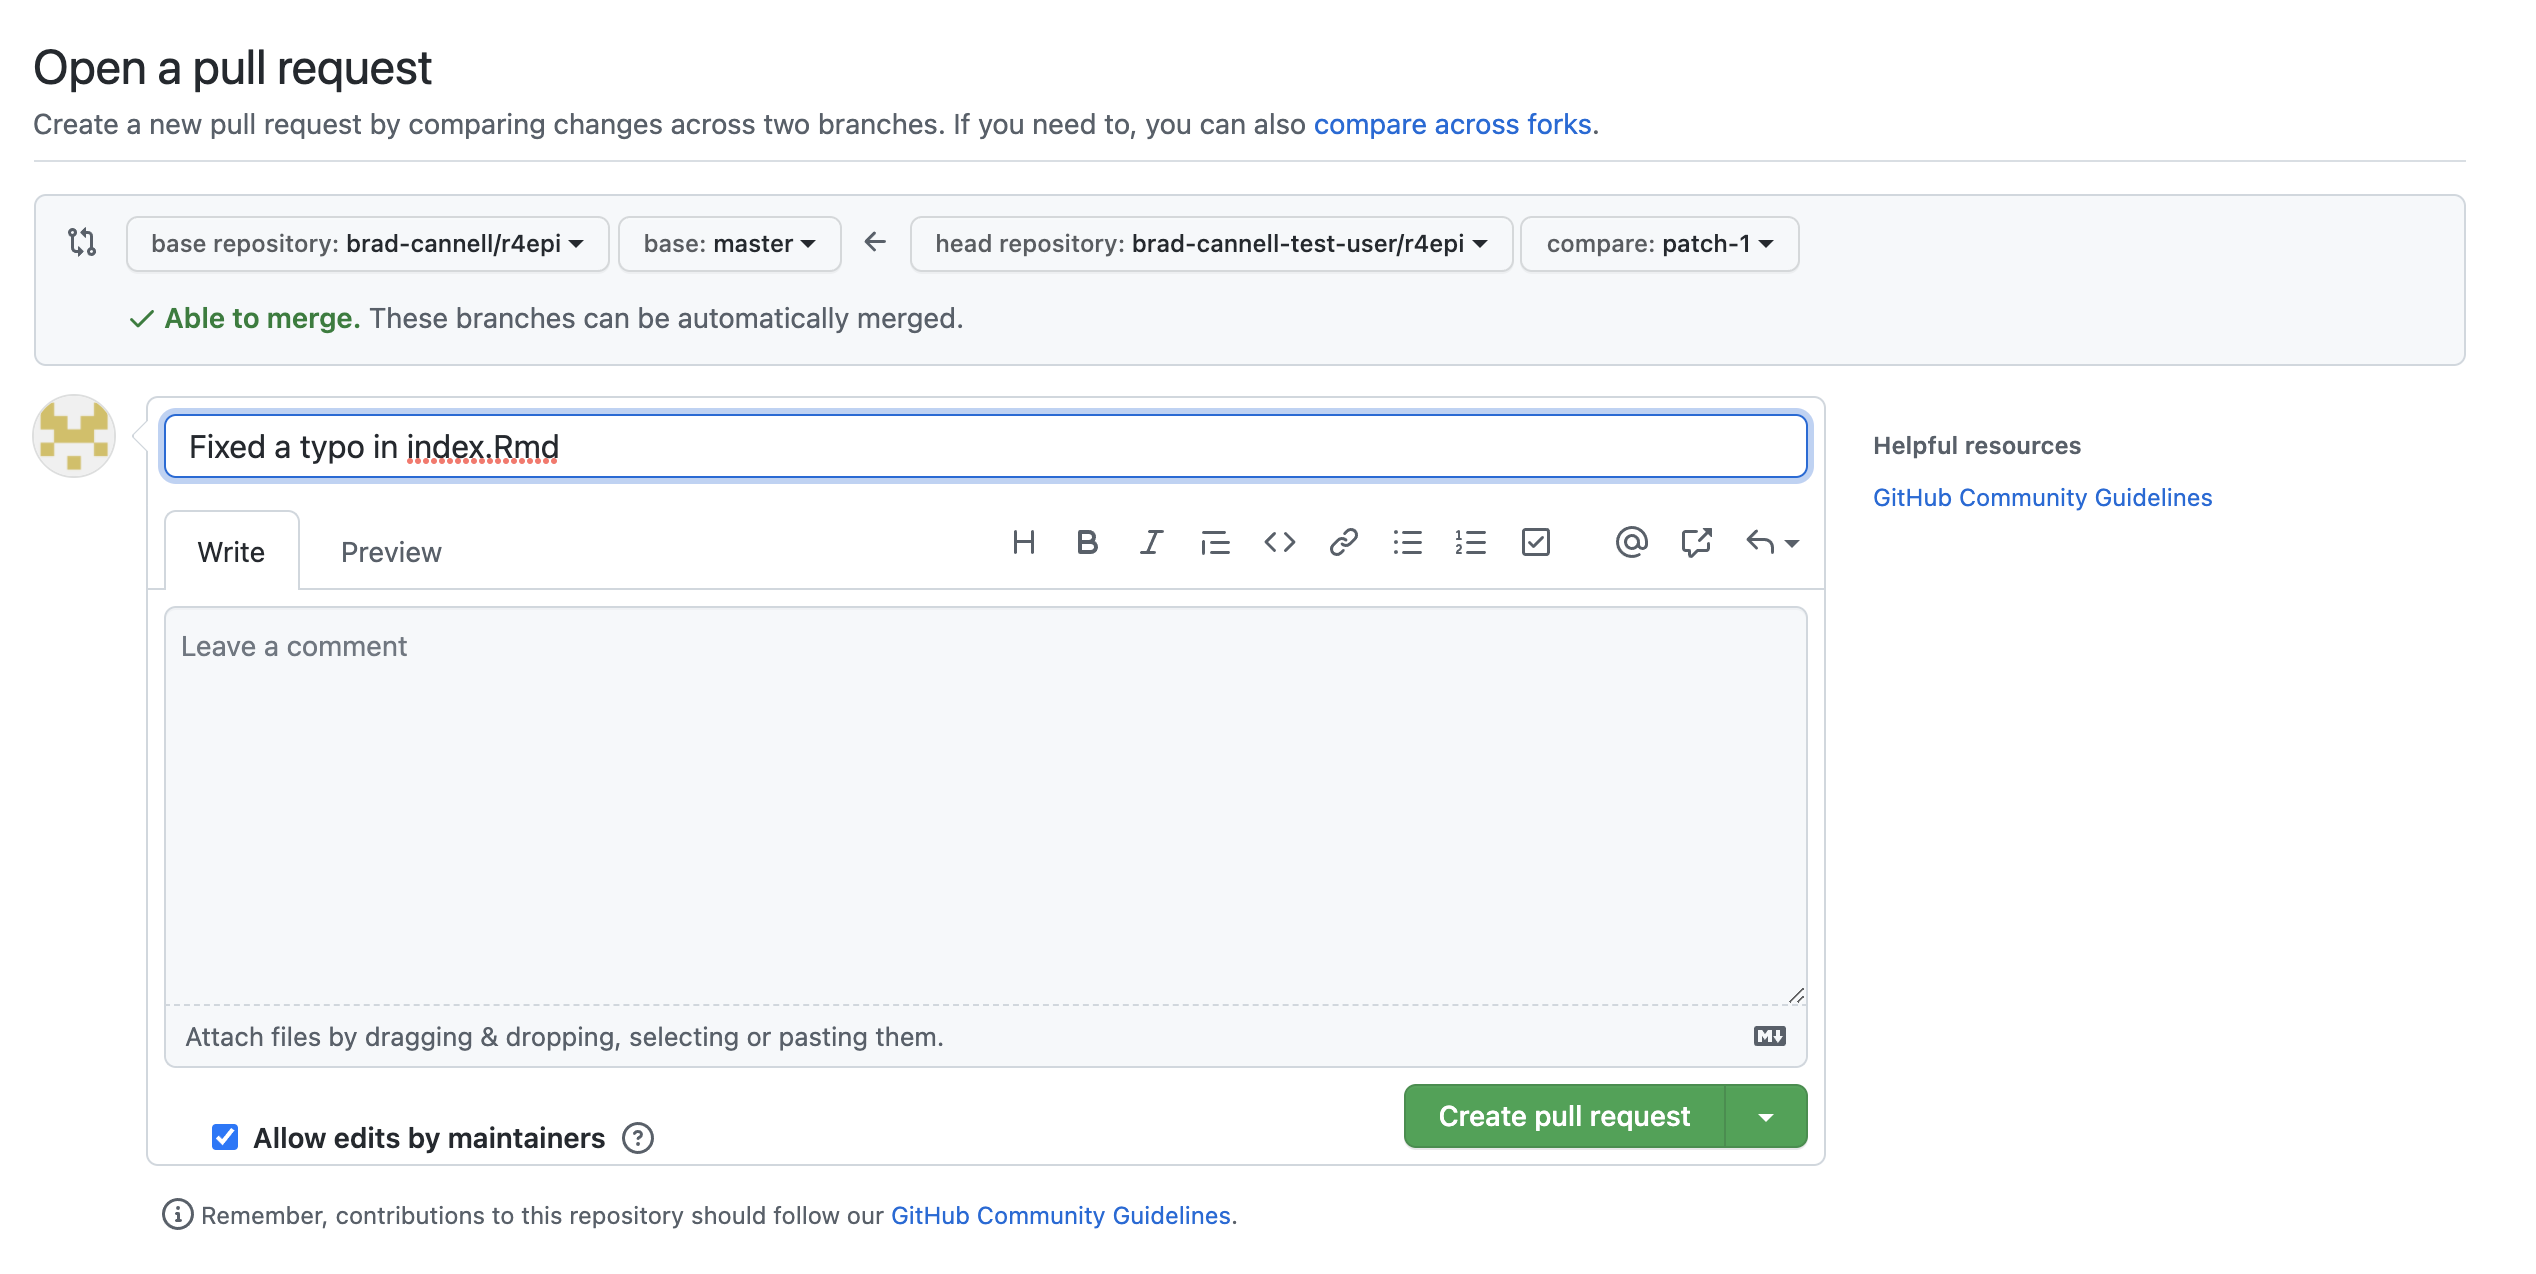
\includegraphics{chapters/contributing/create_pull_request_2.png}

After doing so, you will get one final chance to amend the description
of your proposed changes. If you are happy with the commit message and
description, then click the \texttt{Create\ pull\ request} button one
more time. At this point, your job is done! It is now up to the authors
to review the changes you've proposed and ``pull'' them into the file in
their repository.

In case you are curious, here is what the process looks like on the
authors' end. First, when we open the R4Epi repository page on GitHub,
we will see that there is a new pull request.


\includegraphics{chapters/contributing/create_pull_request_3.png}

When we open the pull request, we can see the proposed changes to the
file.

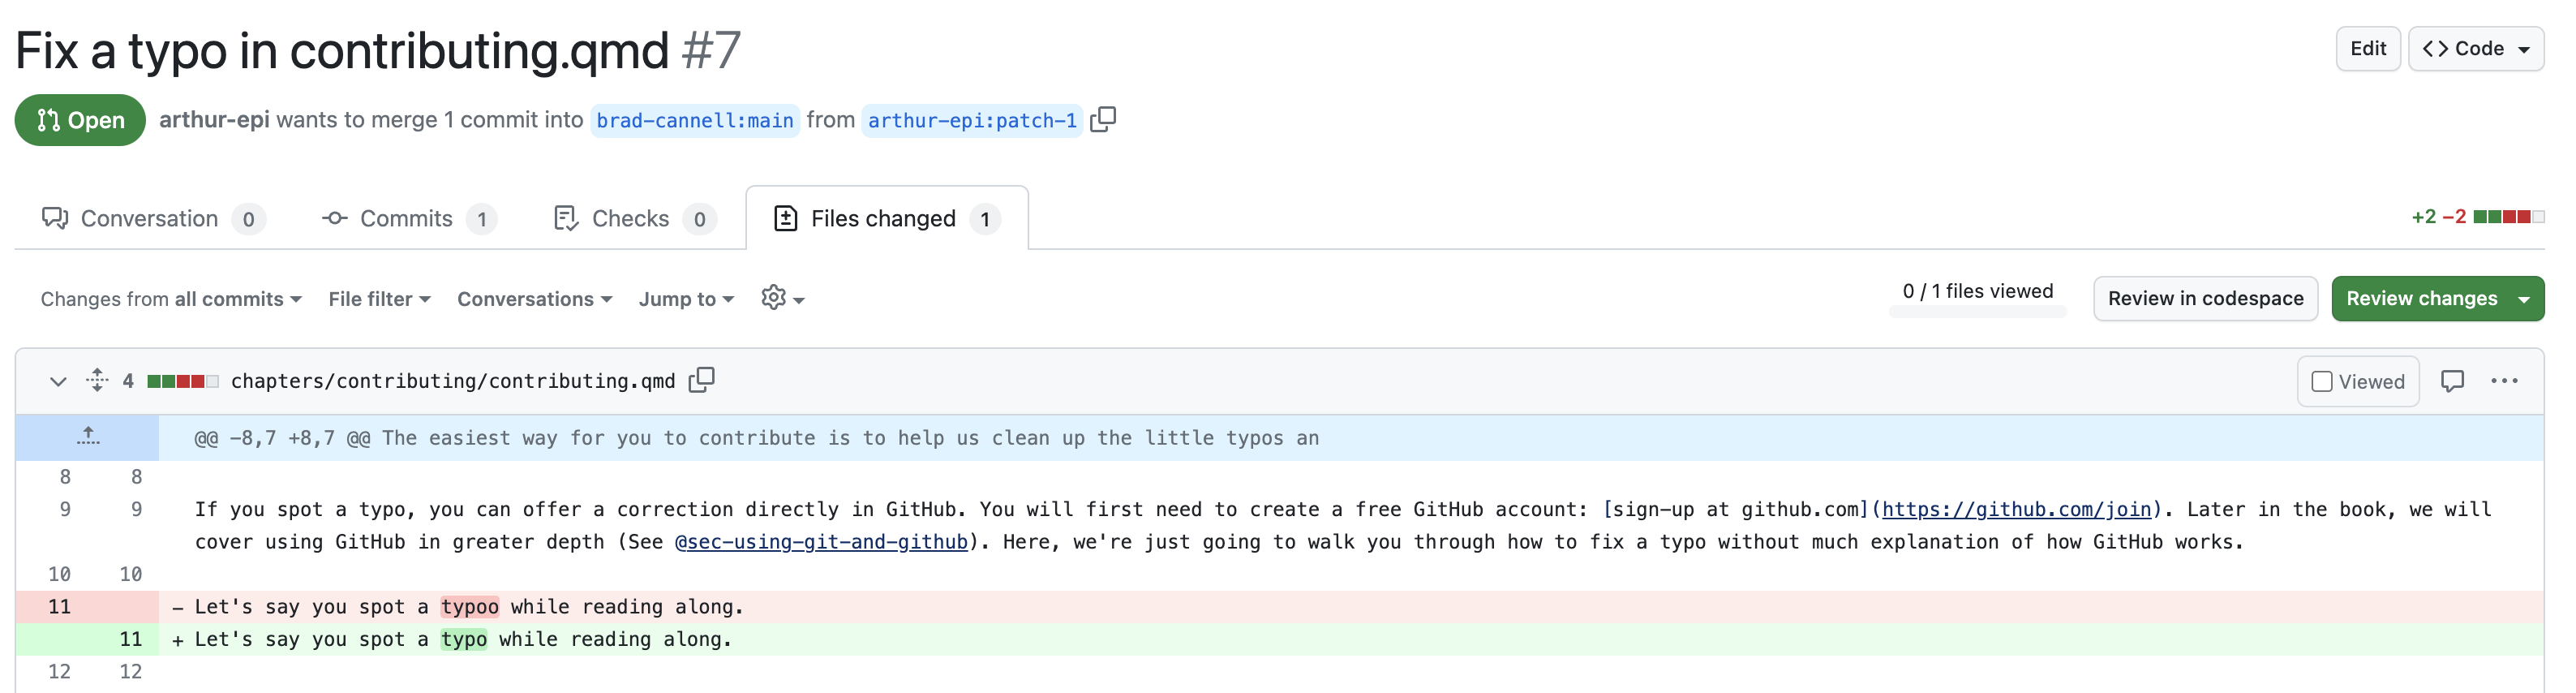
\includegraphics{chapters/contributing/create_pull_request_4.png}

Then, all we have to do is click the
\texttt{Merge\ pull\ request\ button} and the fixed file is ``pulled
in'' to replace the file with the typo.

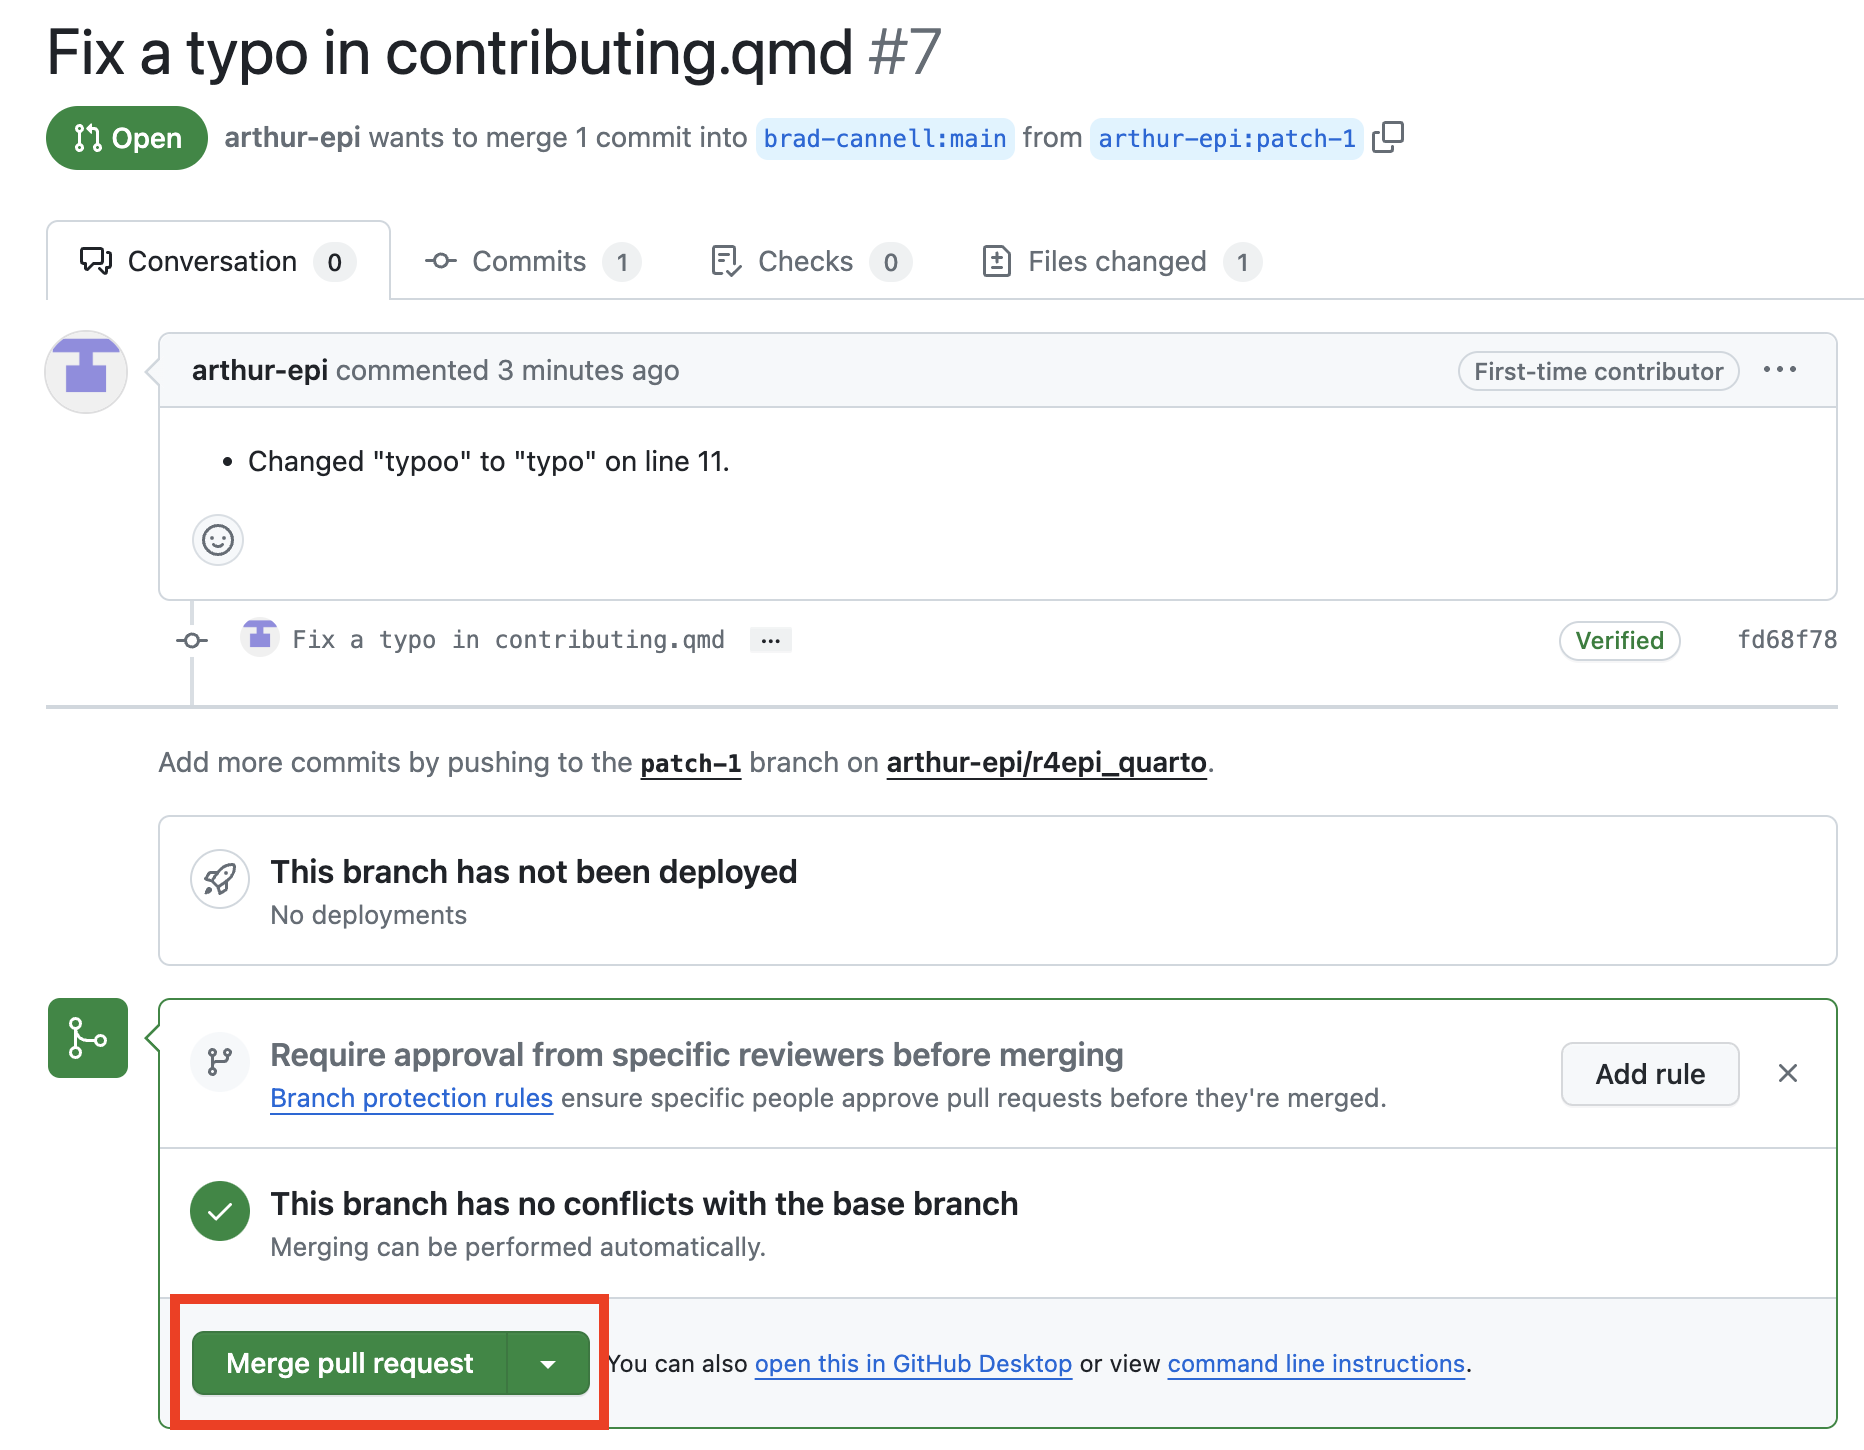
\includegraphics{chapters/contributing/create_pull_request_5.png}

\section*{Issues}\label{issues}
\addcontentsline{toc}{section}{Issues}

\markright{Issues}

There may be times when you see a problem that you don't know how to
fix, but you still want to make the authors aware of. In that case, you
can create an \hyperref[glossary-issue]{issue} in the R4Epi repository.
To do so, navigate to the issue tracker using this link:
https://github.com/brad-cannell/r4epi/issues.

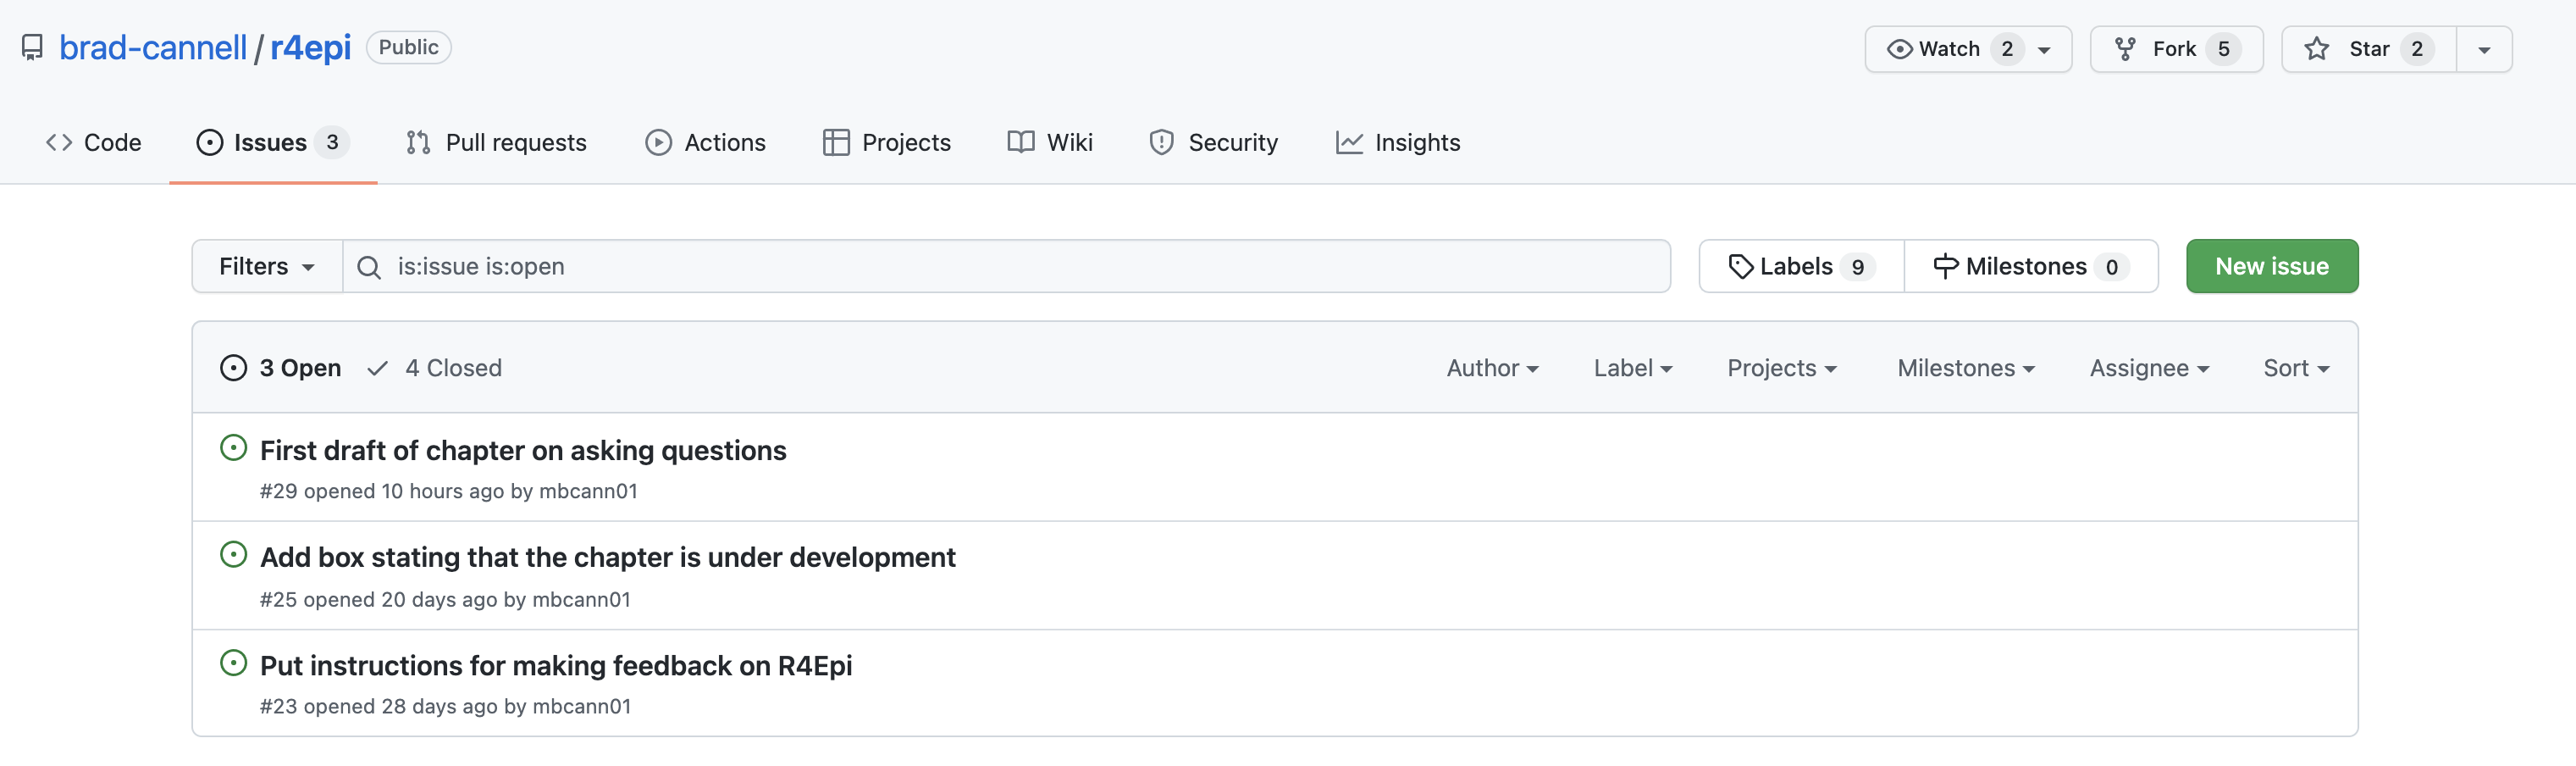
\includegraphics{chapters/contributing/issue_tracker.png}

Once there, you can check to see if someone has already raised the issue
you are concerned about. If not, you can click the green ``New issue''
button to raise it yourself.

Please note that R4Epi uses a
\href{https://contributor-covenant.org/version/2/0/CODE_OF_CONDUCT.html}{Contributor
Code of Conduct}. By contributing to this book, you agree to abide by
its terms.

\section*{License Information}\label{license-information}
\addcontentsline{toc}{section}{License Information}

\markright{License Information}

This book was created by Brad Cannell and is licensed under a Creative
Commons Attribution-NonCommercial-NoDerivatives 4.0 International
License.

\bookmarksetup{startatroot}

\chapter*{About the Authors}\label{about-the-authors}
\addcontentsline{toc}{chapter}{About the Authors}

\markboth{About the Authors}{About the Authors}

\section*{Brad Cannell}\label{brad-cannell}
\addcontentsline{toc}{section}{Brad Cannell}

\markright{Brad Cannell}

\textbf{Michael (Brad) Cannell, PhD, MPH}\\
Associate Professor\\
Elder Mistreatment Lead, UTHealth Institute of Aging\\
Director, Research Informatics Core, Cizik Nursing Research Institute\\
UTHealth Houston\\
McGovern Medical School\\
Joan and Stanford Alexander Division of Geriatric \& Palliative
Medicine\\
\href{https://www.bradcannell.com}{www.bradcannell.com}

Dr.~Cannell received his PhD in Epidemiology, and Graduate Certificate
in Gerontology, in 2013 from the University of Florida. He received his
MPH with a concentration in Epidemiology from the University of
Louisville in 2009, and his BA in Political Science and Marketing from
the University of North Texas in 2005. During his doctoral studies, he
was a Graduate Research Assistant for the Florida Office on Disability
and Health, an affiliated scholar with the Claude D. Pepper Older
Americans Independence Center, and a student-inducted member of the
Delta Omega Honorary Society in Public Health. In 2016, Dr.~Cannell
received a Graduate Certificate in Predictive Analytics from the
University of Maryland University College, and a Certificate in Big Data
and Social Analytics from the Massachusetts Institute of Technology.

He previously held professional staff positions in the Louisville Metro
Health Department and the Northern Kentucky Independent District Health
Department. He spent three years as a project epidemiologist for the
Florida Office on Disability and Health at the University of Florida. He
also served as an Environmental Science Officer in the United States
Army Reserves from 2009 to 2013.

Dr.~Cannell's research is broadly focused on healthy aging and
health-related quality of life. Specifically, he has published research
focusing on preservation of physical and cognitive function, living and
aging with disability, and understanding and preventing elder
mistreatment. Additionally, he has a strong background and training in
epidemiologic methods and predictive analytics. He has been principal or
co-investigator on multiple trials and observational studies in
community and healthcare settings. He is currently the principal
investigator on multiple data-driven federally funded projects that
utilize technological solutions to public health issues in novel ways.

\textbf{Contact}\\
Connect with Dr.~Cannell and follow his work.\\

\includegraphics[width=2em,height=2em]{chapters/about_the_authors/about_the_authors_files/figure-pdf/fa-icon-a4a233699ebb8edeaca4e7ae0455099b.pdf}

\includegraphics[width=1.75em,height=2em]{chapters/about_the_authors/about_the_authors_files/figure-pdf/fa-icon-d19241927d9e636802f0f0caca52c0af.pdf}

\includegraphics[width=1.75em,height=2em]{chapters/about_the_authors/about_the_authors_files/figure-pdf/fa-icon-f2455331e499245af38ff1988a0023d4.pdf}

\includegraphics[width=1.75em,height=2em]{chapters/about_the_authors/about_the_authors_files/figure-pdf/fa-icon-1cbfc0b82b7e84c9b17b238bfd9a886e.pdf}

\section*{Melvin Livingston}\label{melvin-livingston}
\addcontentsline{toc}{section}{Melvin Livingston}

\markright{Melvin Livingston}

\textbf{Melvin (Doug) Livingston, PhD}\\
Research Associate Professor\\
Department of Behavioral, Social, and Health Education Sciences\\
Emory University Woodruff Health Sciences Center\\
Rollins School of Public Health\\
\href{https://sph.emory.edu/faculty/profile/index.php?FID=melvin-livingston-8970}{Dr.~Livingston's
Faculty Profile}

Dr.~Livingston is a methodologist with expertise in the the application
of quasi-experimental design principals to the evaluation for both
community interventions and state policies. He has particular expertise
in time series modeling, mixed effects modeling, econometric methods,
and power analysis. As part of his work involving community trials, he
has been the statistician on the long term follow-up study of a school
based cluster randomized trial in low-income communities with a focus on
explaining the etiology of risky alcohol, drug, and sexual behaviors.
Additionally, he was the statistician for a longitudinal study examining
the etiology of alcohol use among racially diverse and economically
disadvantaged urban youth, and co-investigator for a NIAAA- and
NIDA-funded trial to prevent alcohol use and alcohol-related problems
among youth living in high-risk, low-income communities within the
Cherokee Nation. Prevention work at the community level led him to an
interest in the impact of state and federal socioeconomic policies on
health outcomes. He is a Co-Investigator of a 50-state, 30-year study of
effects of state-level economic and education policies on a diverse set
of public health outcomes, explicitly examining differential effects
across disadvantaged subgroups of the population.

His current research interests center around the application of
quasi-experimental design and econometric methods to the evaluation of
the health effects of state and federal policy.

\textbf{Contact}\\
Connect with Dr.~Livingston and follow his work.\\

\includegraphics[width=2em,height=2em]{chapters/about_the_authors/about_the_authors_files/figure-pdf/fa-icon-a4a233699ebb8edeaca4e7ae0455099b.pdf}

\includegraphics[width=1.75em,height=2em]{chapters/about_the_authors/about_the_authors_files/figure-pdf/fa-icon-ab37b36564b32e84e458655a90d49135.pdf}

\part{Getting Started}

\chapter{Installing R and RStudio}\label{installing-r-and-rstudio}

Before we can do any programming with \hyperref[glossary-r]{R}, we first
have to download it to our computer. Fortunately, R is free, easy to
install, and runs on all major operating systems (i.e., Mac and
Windows). However, R is even easier to use as when we combine it with
another program called \hyperref[glossary-rstudio]{RStudio}.
Fortunately, RStudio is also free and will also run on all major
operating systems.

At this point, you may be wondering what R is, what RStudio is, and how
they are related. We will answer those questions in the near future.
However, in the interest of keeping things brief and simple, We're not
going to get into them right now. Instead, all you have to worry about
is getting the R programming language and the RStudio IDE (IDE is short
for integrated development environment) downloaded and installed on your
computer. The steps involved are slightly different depending on whether
you are using a Mac or a PC (i.e., Windows). Therefore, please feel free
to use the table of contents on the right-hand side of the screen to
navigate directly to the instructions that you need for your computer.

\begin{tcolorbox}[enhanced jigsaw, rightrule=.15mm, breakable, colback=white, bottomtitle=1mm, title=\textcolor{quarto-callout-note-color}{\faInfo}\hspace{0.5em}{Note}, colframe=quarto-callout-note-color-frame, opacityback=0, coltitle=black, colbacktitle=quarto-callout-note-color!10!white, opacitybacktitle=0.6, toptitle=1mm, bottomrule=.15mm, left=2mm, leftrule=.75mm, titlerule=0mm, toprule=.15mm, arc=.35mm]

In this chapter, we cover how to download and install R and RStudio on
both Mac and PC. However, the screenshots in all following chapters will
be from a Mac. The good news is that RStudio operates almost identically
on Mac and PC.

\end{tcolorbox}

\textbf{Step 1:} Regardless of which operating system you are using,
please make sure your computer is on, properly functioning, connected to
the internet, and has enough space on your hard drive to save R and
RStudio.

\section{Download and install on a
Mac}\label{download-and-install-on-a-mac}

\textbf{Step 2:} Navigate to the Comprehensive R Archive Network (CRAN),
which is located at https://cran.r-project.org/.

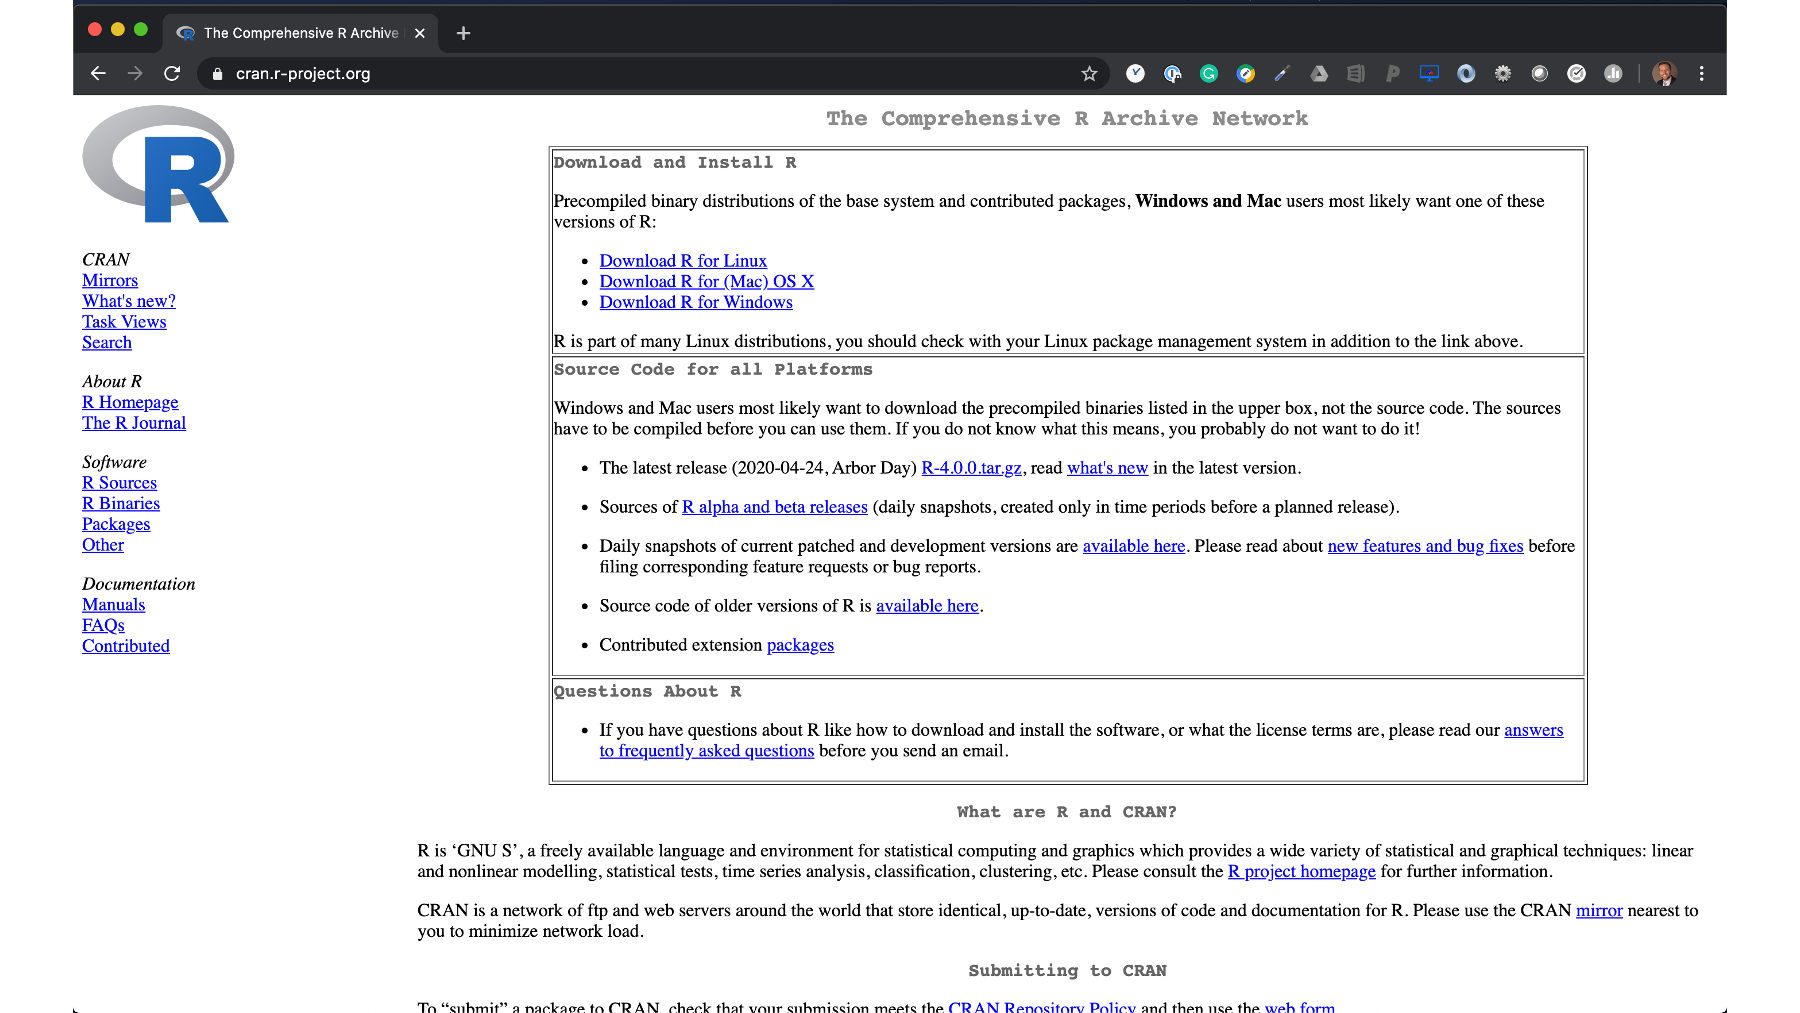
\includegraphics{chapters/installing_r_and_rstudio/mac_cran.png}

\textbf{Step 3:} Click on Download R for macOS.

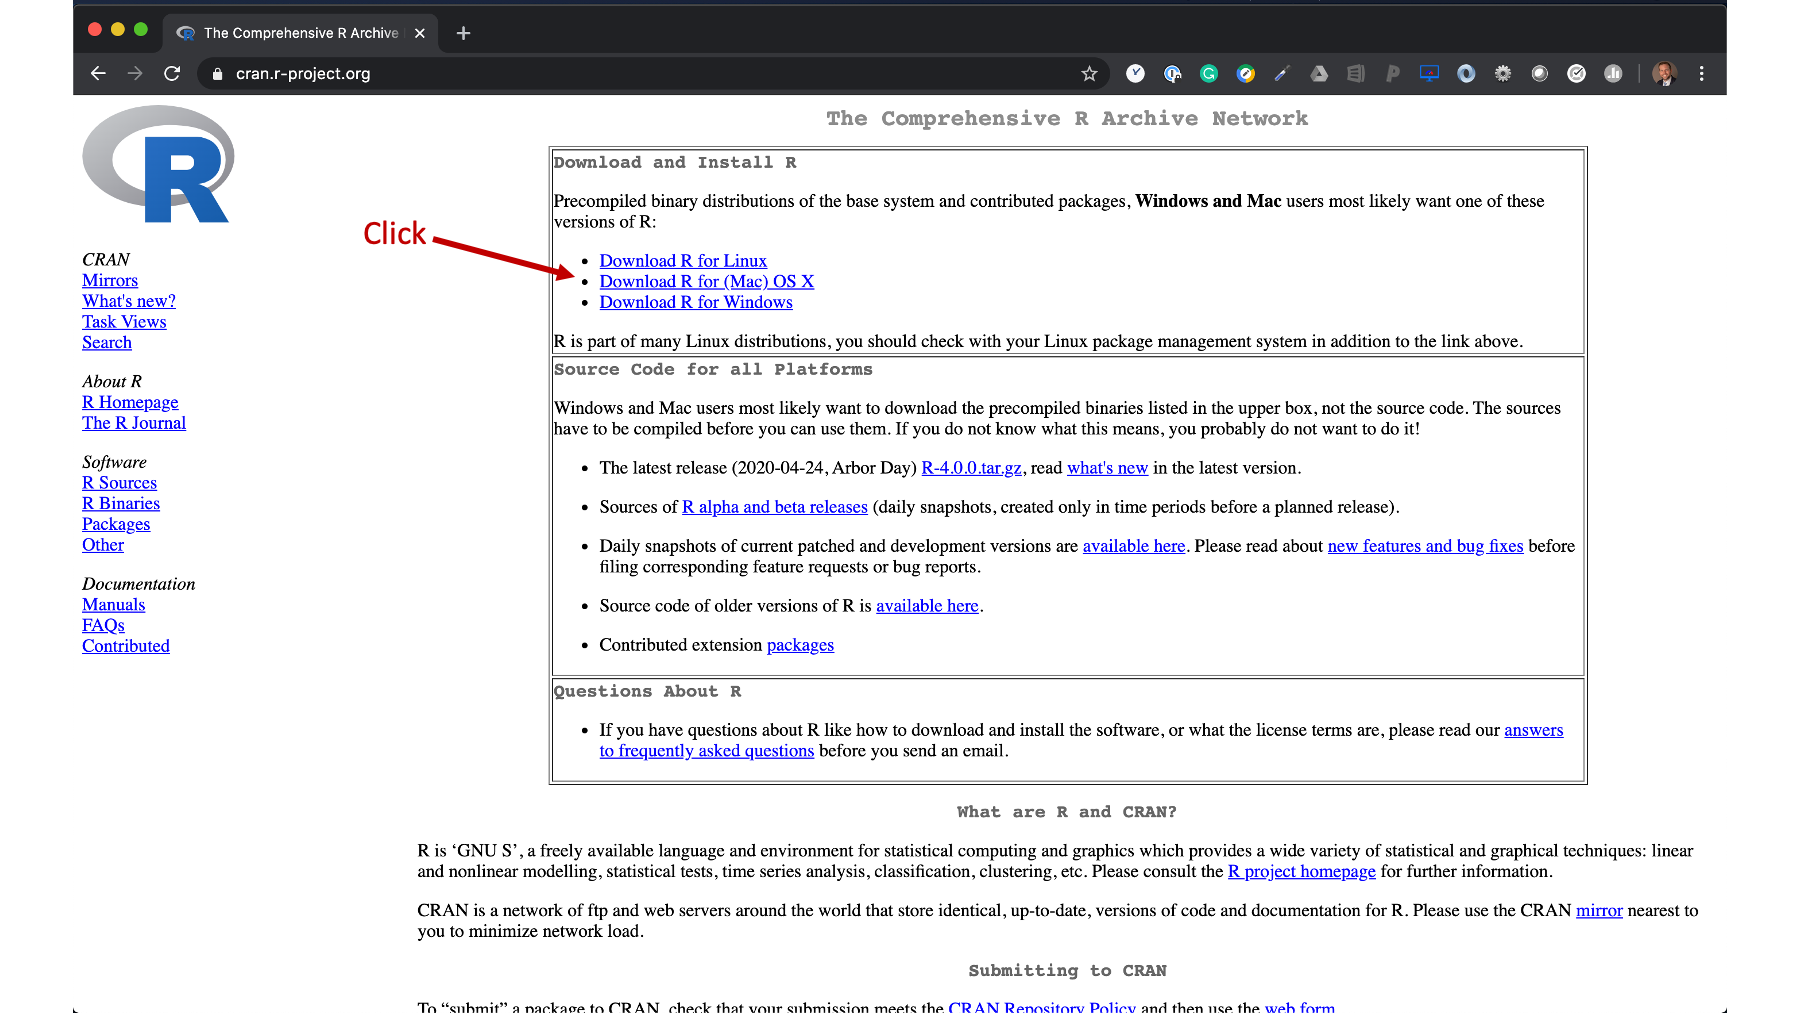
\includegraphics{chapters/installing_r_and_rstudio/mac_download_r.png}

\textbf{Step 4:} Click on the link for the latest version of R. As you
are reading this, the newest version may be different than the version
you see in this picture, but the location of the newest version should
be roughly in the same place -- the middle of the screen under ``Latest
release:''. After clicking the link, R should start to download to your
computer automatically.

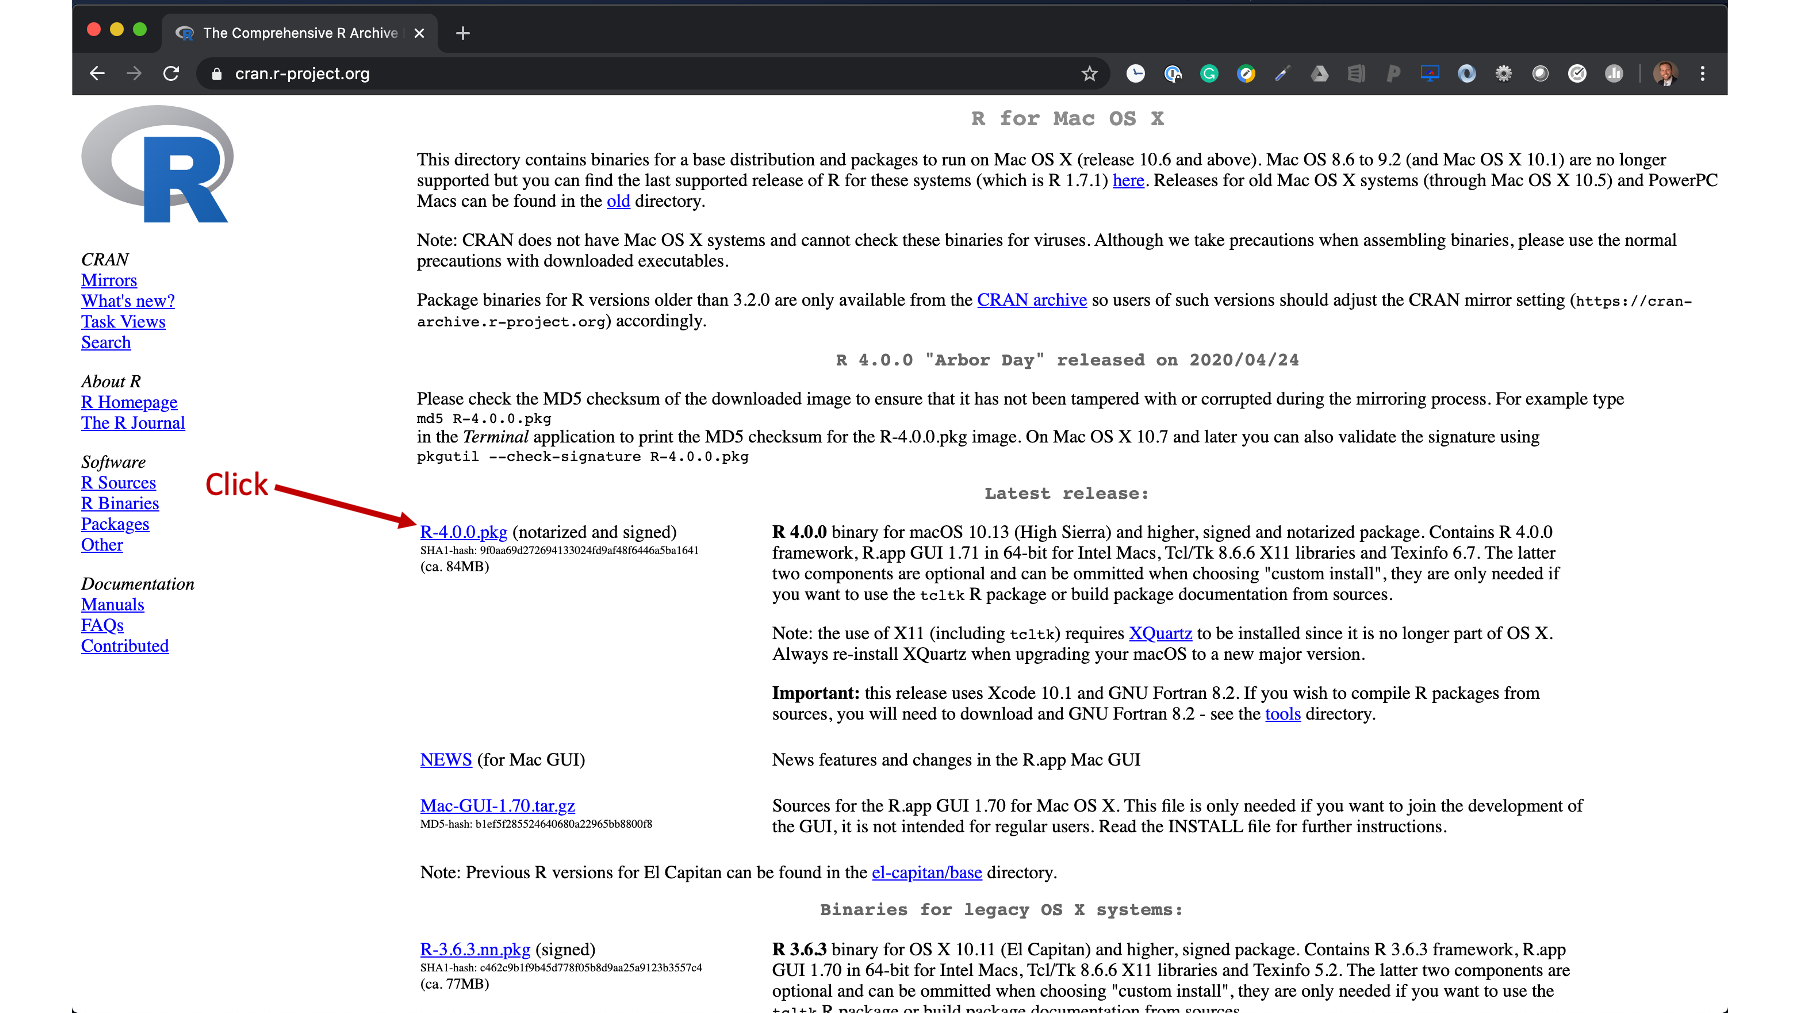
\includegraphics{chapters/installing_r_and_rstudio/mac_r_version.png}

\textbf{Step 5:} Locate the package file you just downloaded and double
click it. Unless you've changed your download settings, this file will
probably be in your ``downloads'' folder. That is the default location
for most web browsers. After you locate the file, just double click it.

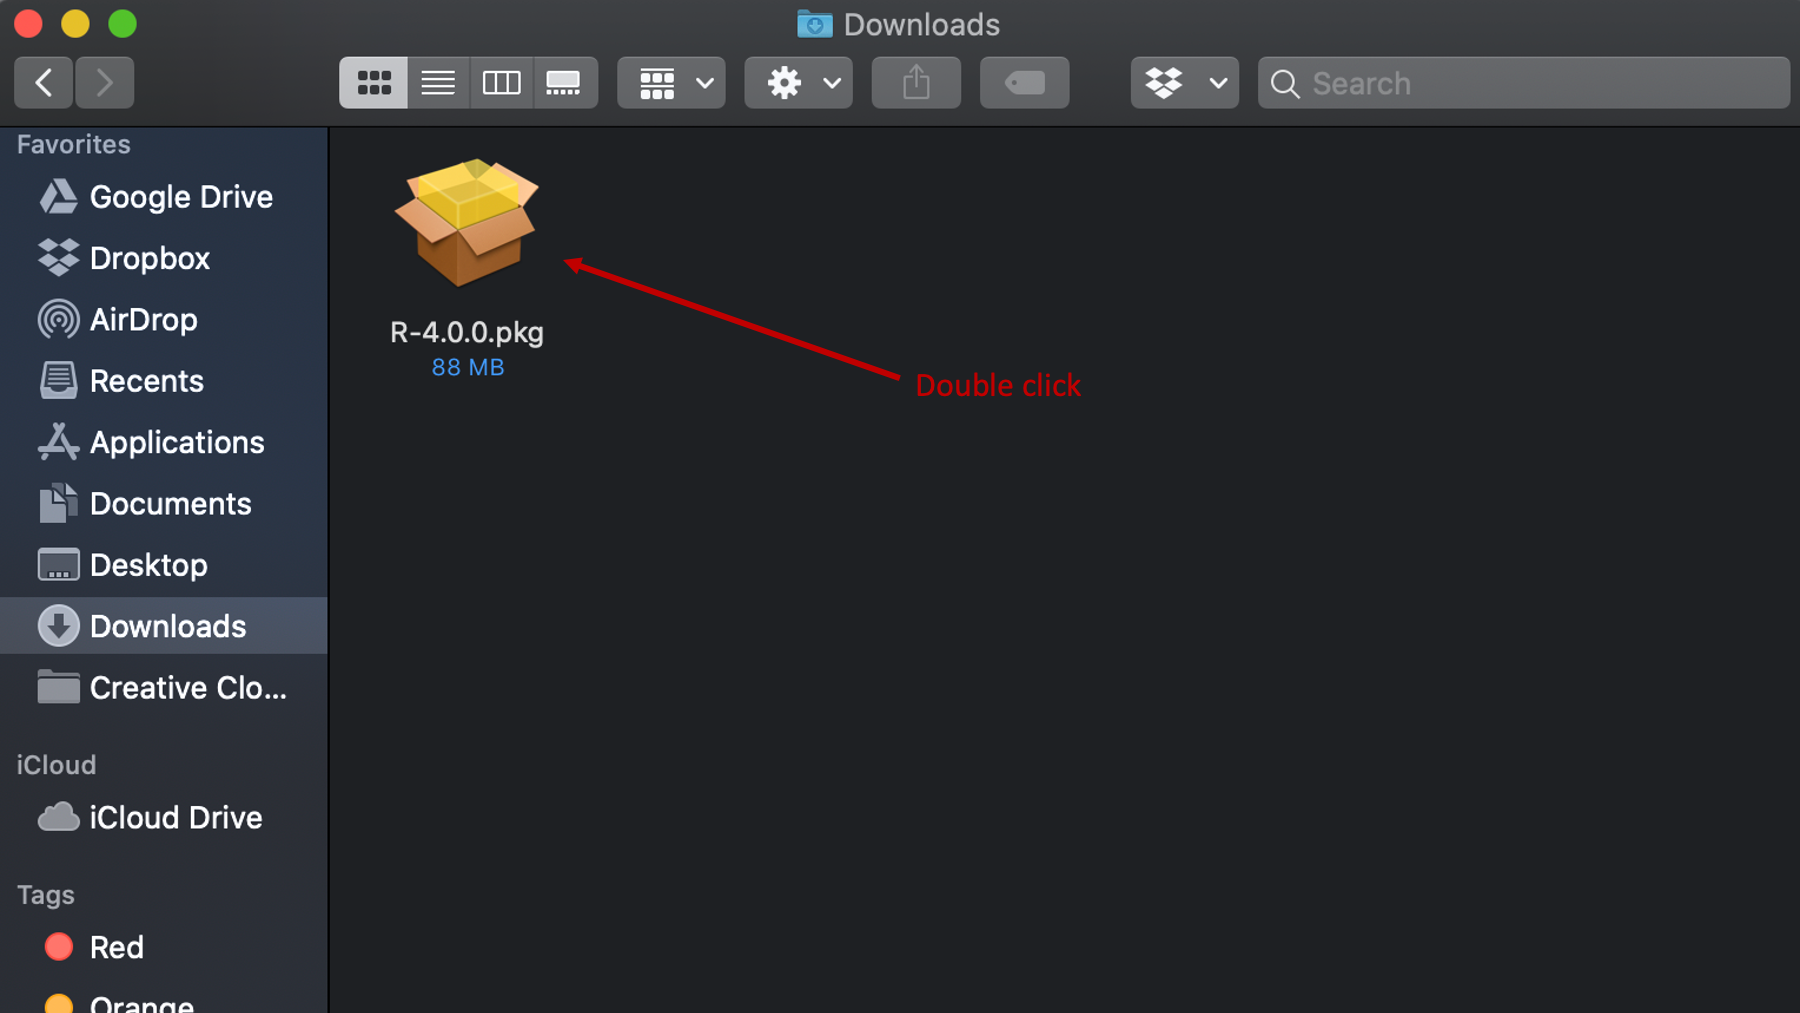
\includegraphics{chapters/installing_r_and_rstudio/mac_install_r1.png}

\textbf{Step 6:} A dialogue box will open and ask you to make some
decisions about how and where you want to install R on your computer. We
typically just click ``continue'' at every step without changing any of
the default options.

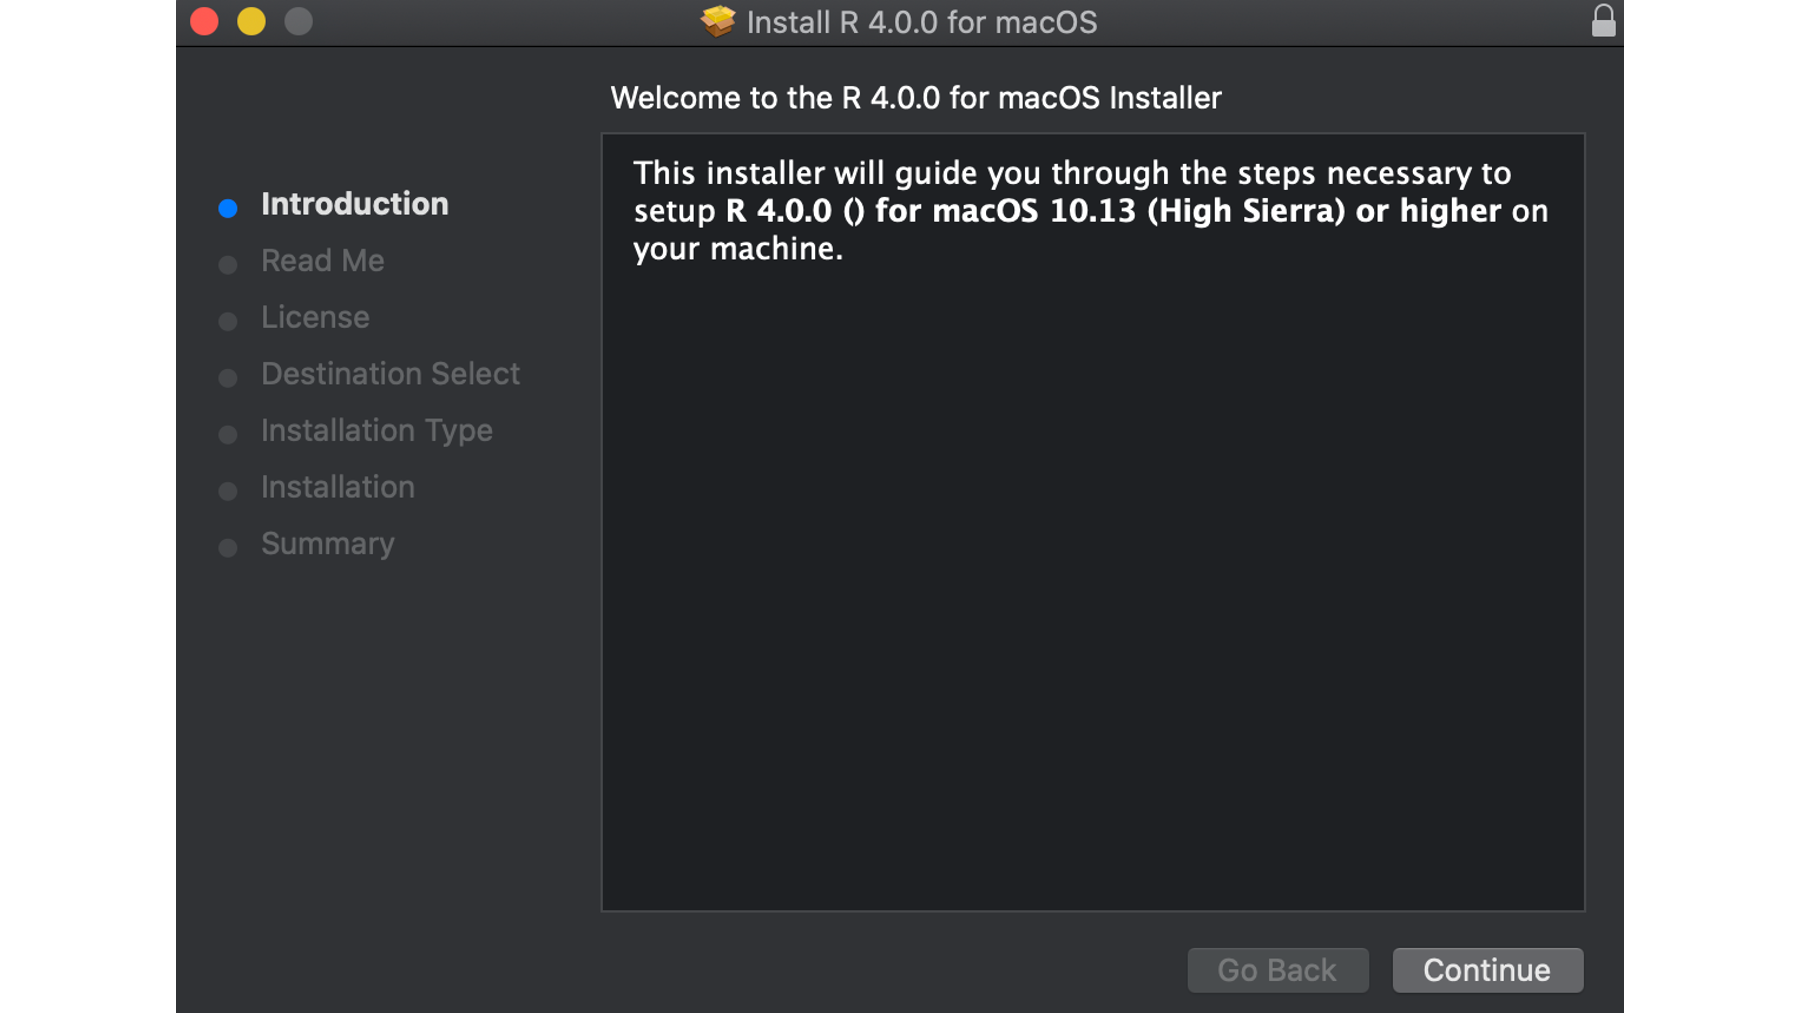
\includegraphics{chapters/installing_r_and_rstudio/mac_install_r2.png}

If R installed properly, you should now see it in your applications
folder.


\includegraphics{chapters/installing_r_and_rstudio/mac_view_r.png}

\textbf{Step 7:} Now, we need to install the RStudio IDE. To do this,
navigate to the RStudio desktop download website, which is located at
https://posit.co/download/rstudio-desktop/. On that page, click the
button to download the latest version of RStudio for your computer. Note
that the website may look different that what you see in the screenshot
below because websites change over time.

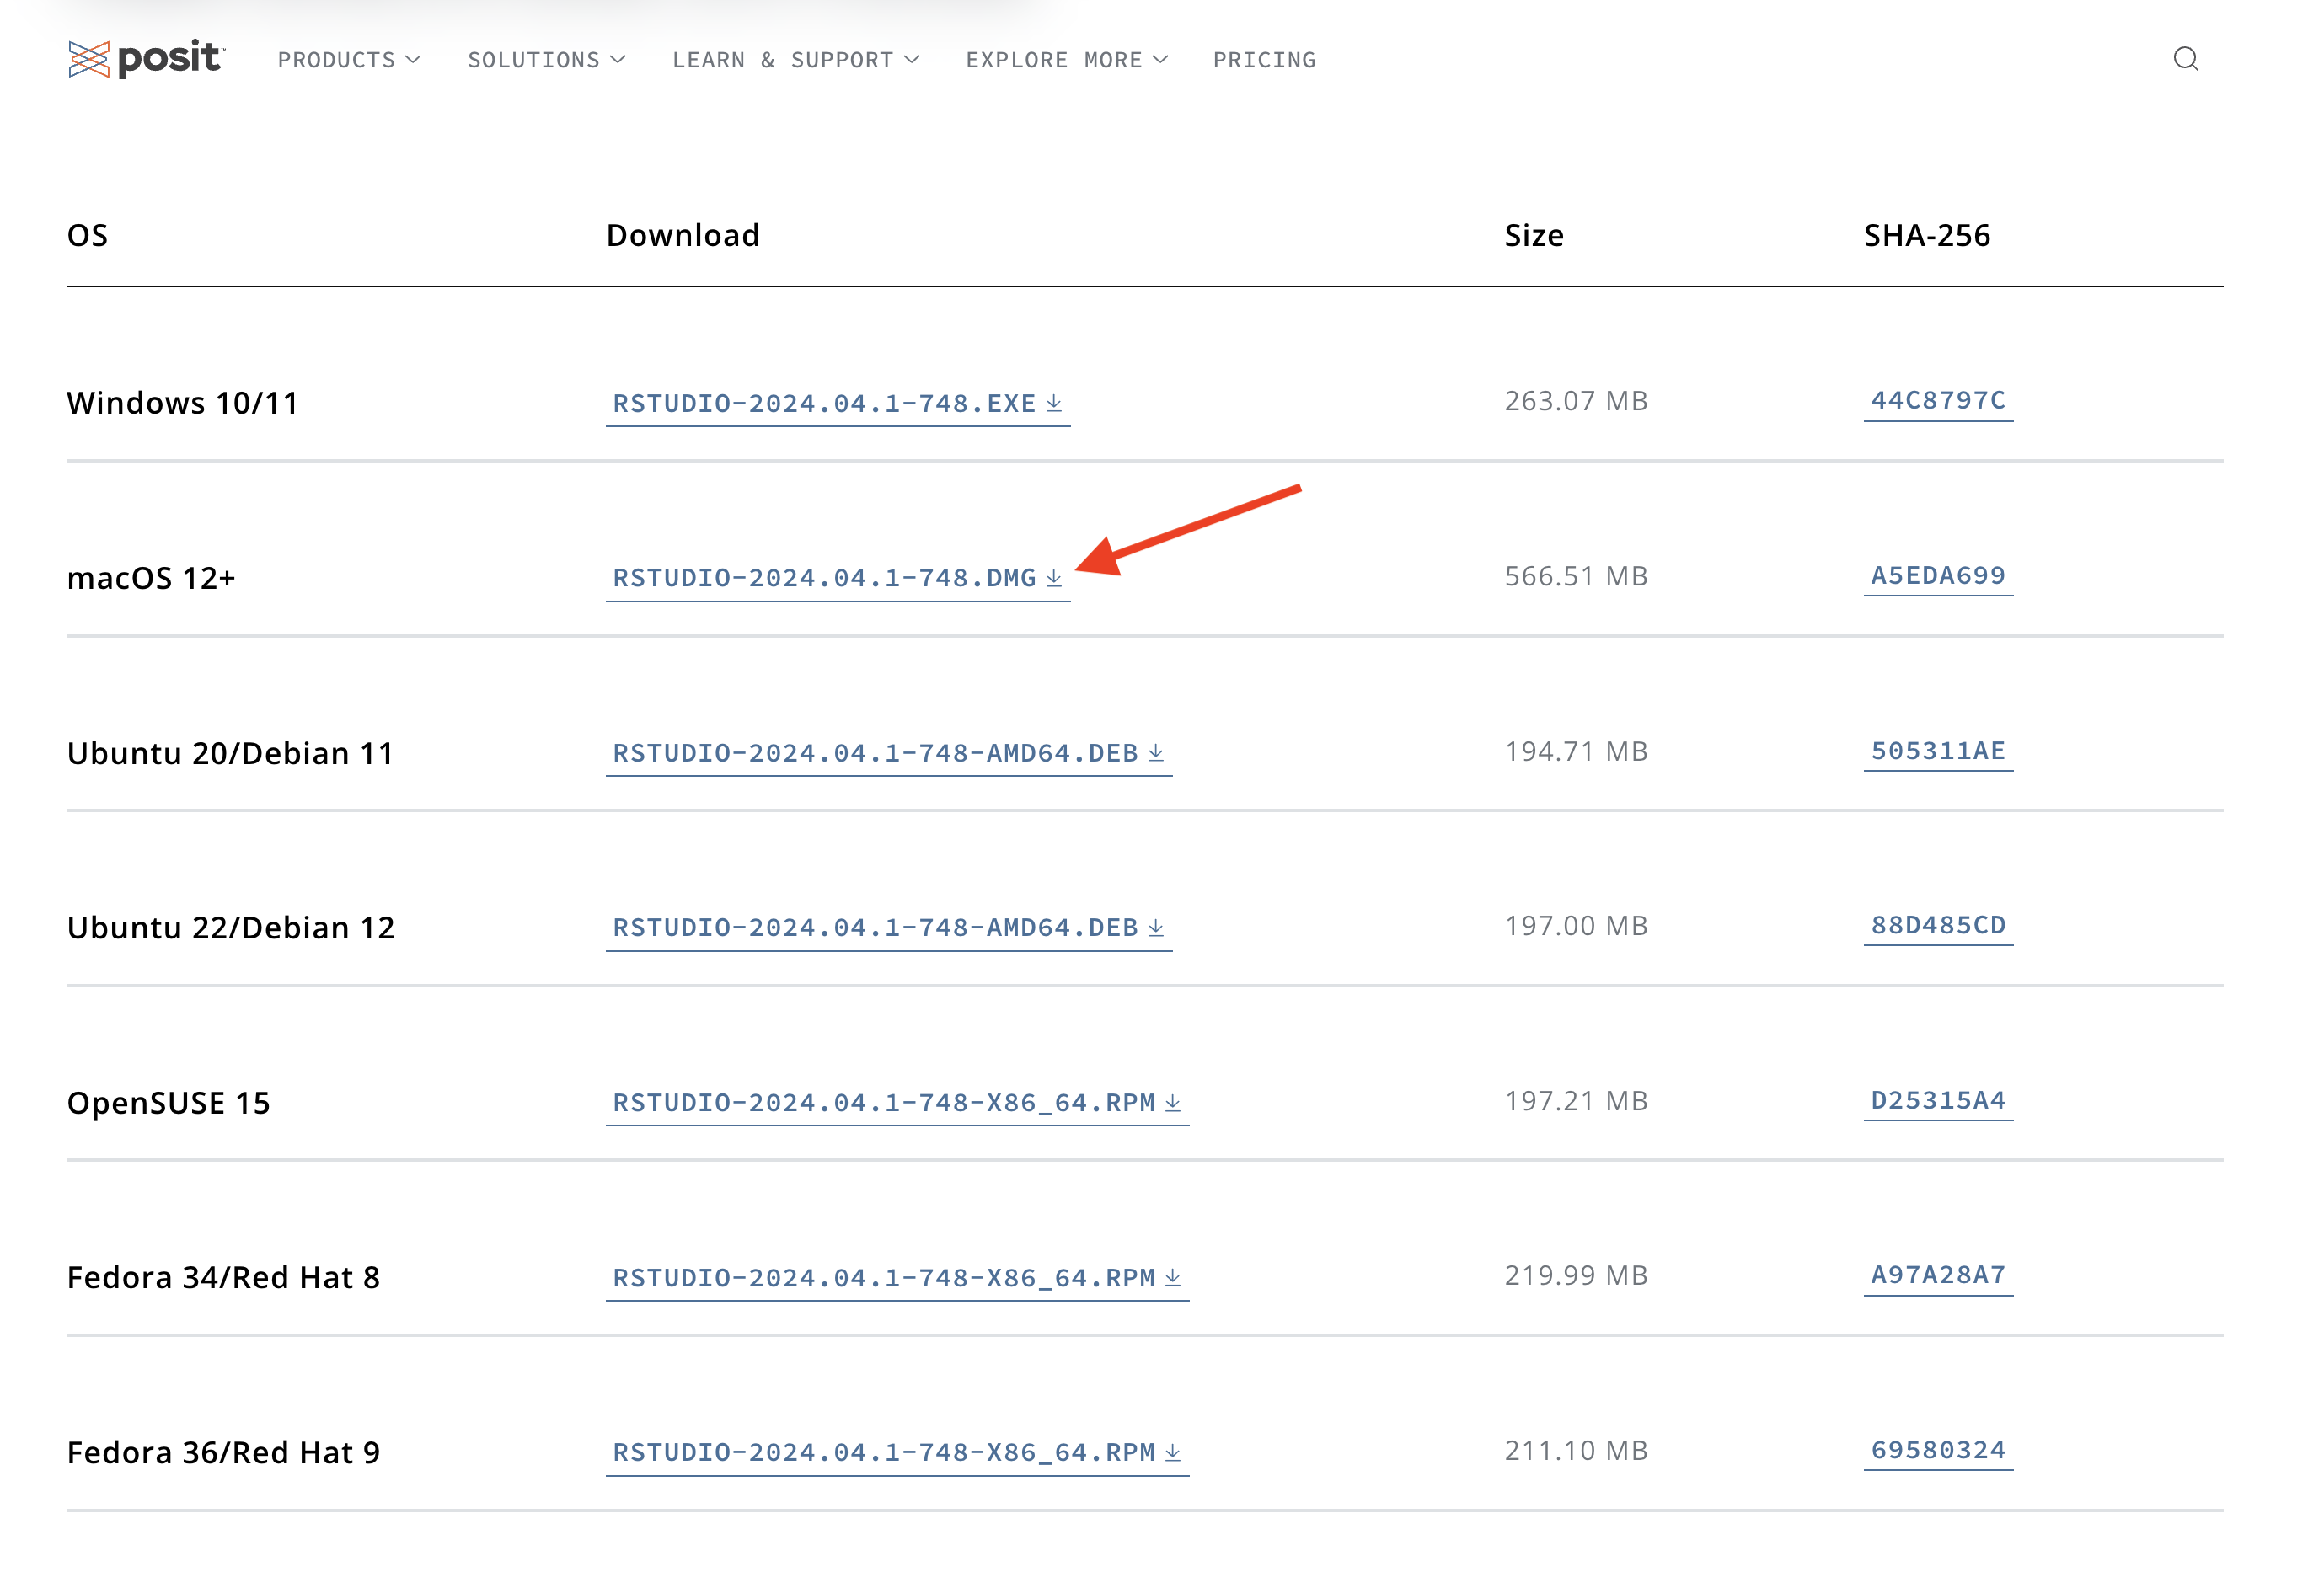
\includegraphics{chapters/installing_r_and_rstudio/mac_download_rstudio1.png}

\textbf{Step 8:} Again, locate the DMG file you just downloaded and
double click it. Unless you've changed your download settings, this file
should be in the same location as the R package file you already
downloaded.

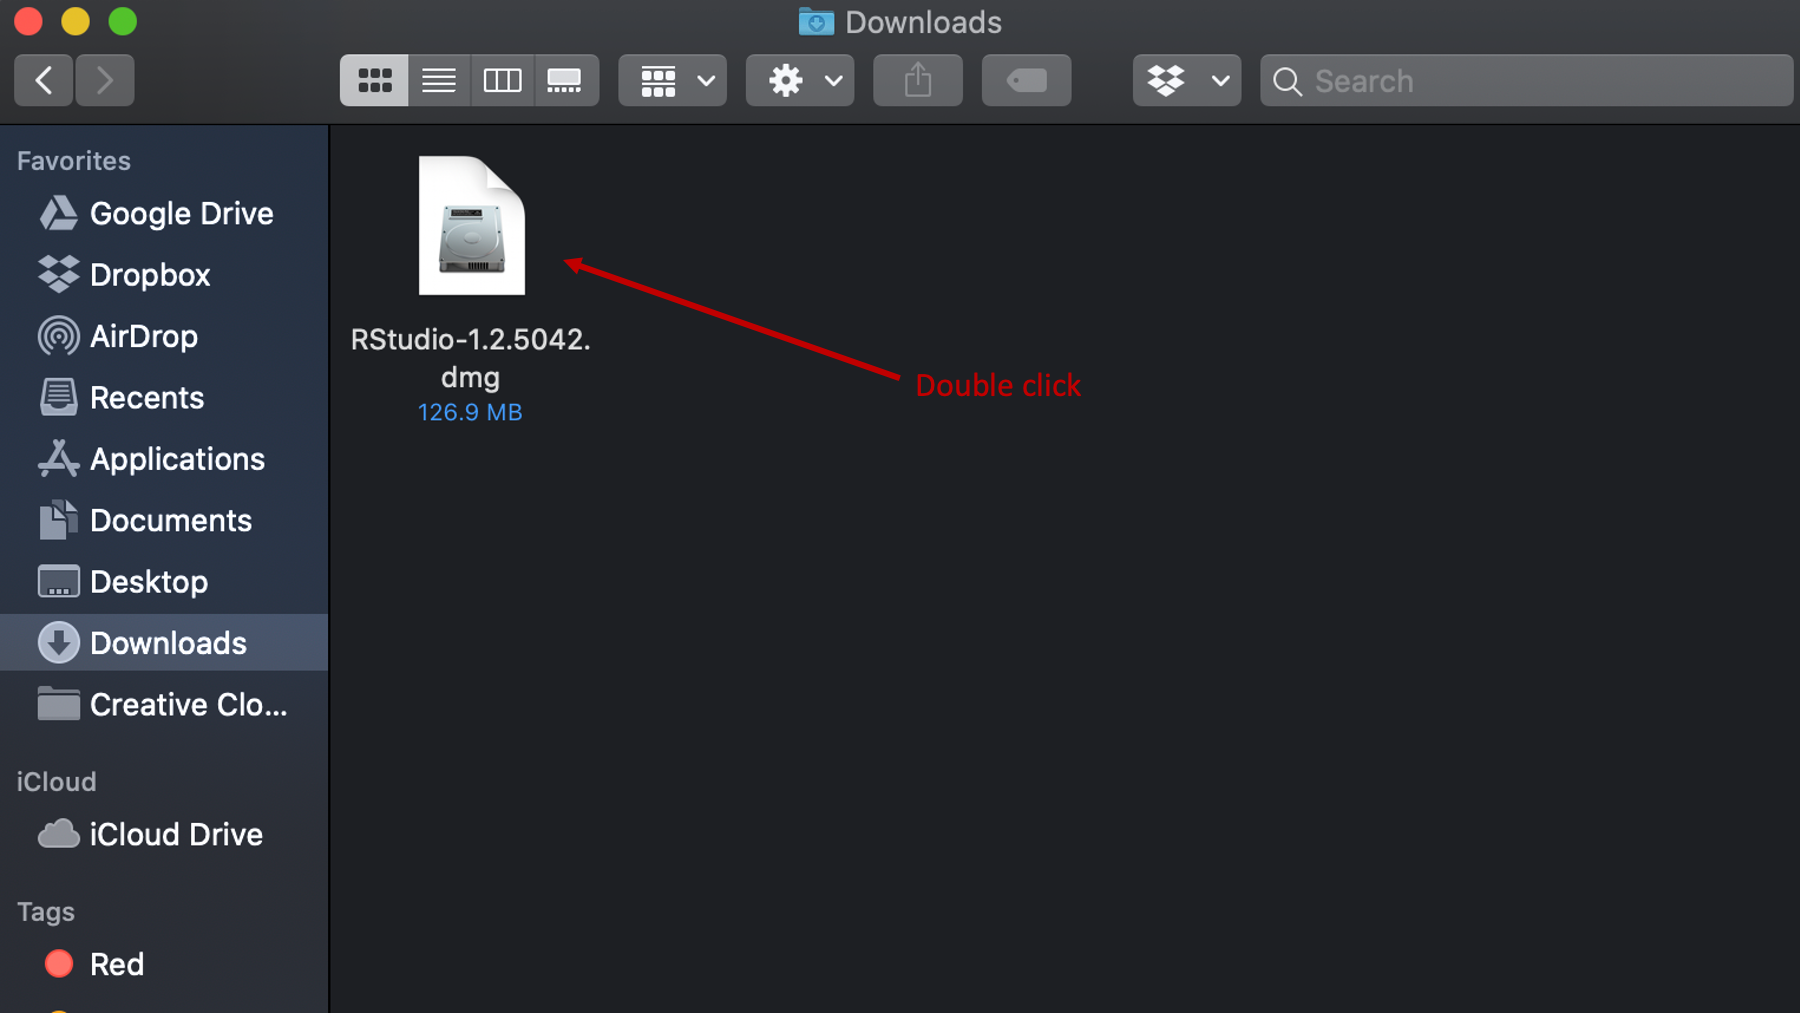
\includegraphics{chapters/installing_r_and_rstudio/mac_install_rstudio1.png}

\textbf{Step 9:} A new finder window should automatically pop up that
looks like the one you see below. Click on the RStudio icon and drag it
into the Applications folder.

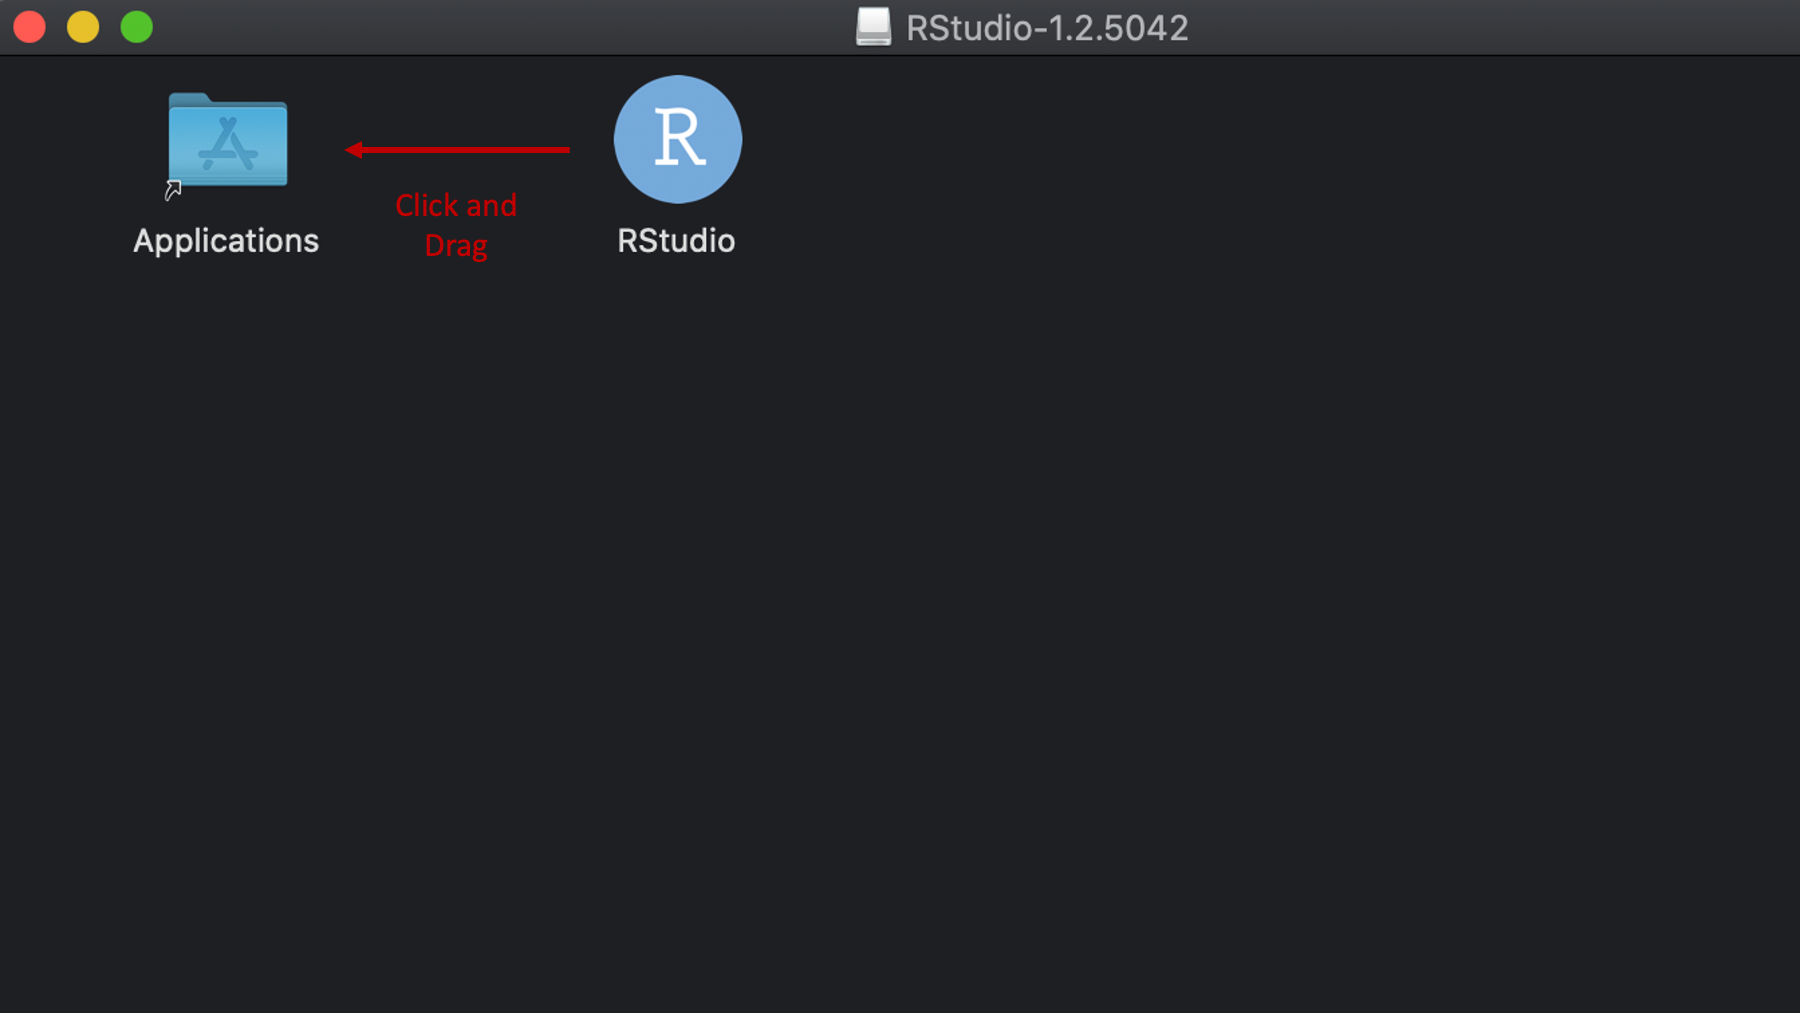
\includegraphics{chapters/installing_r_and_rstudio/mac_install_rstudio2.png}

You should now see RStudio in your Applications folder. Double click the
icon to open RStudio.


\includegraphics{chapters/installing_r_and_rstudio/mac_open_rstudio.png}

If this warning pops up, just click Open.

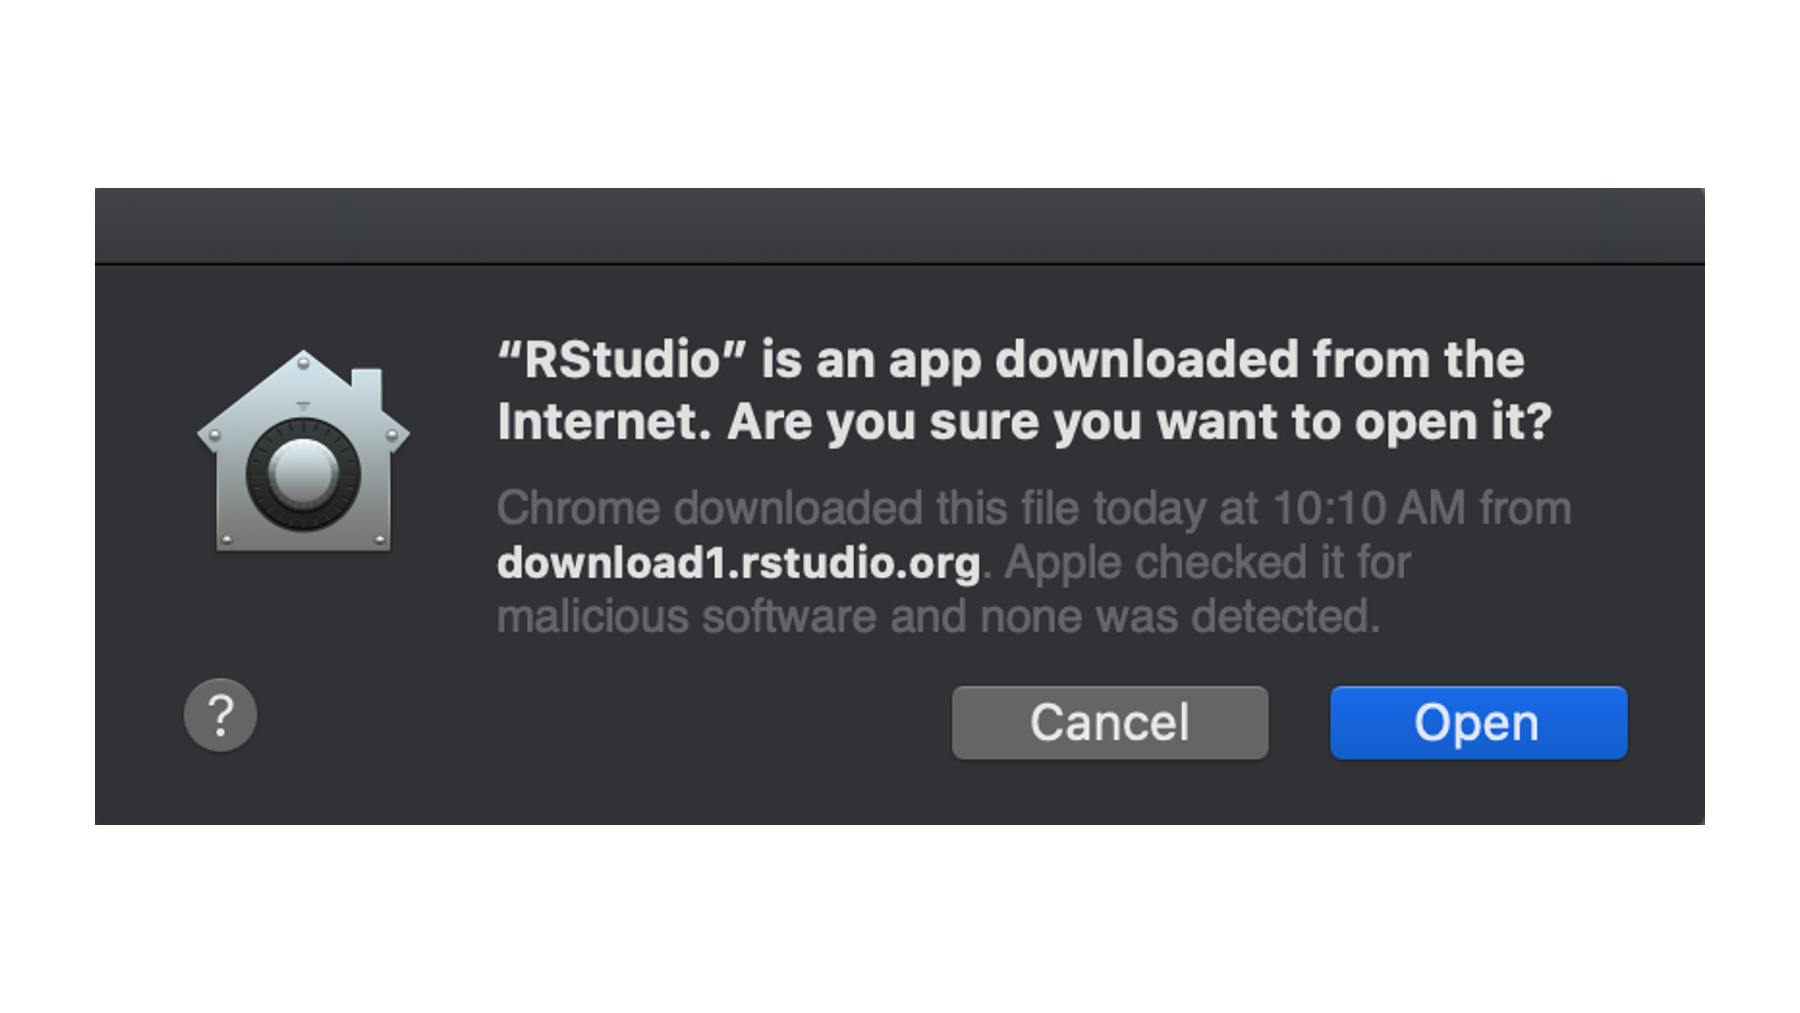
\includegraphics{chapters/installing_r_and_rstudio/mac_open_warning.png}

The RStudio IDE should open and look something like the window you see
here. If so, you are good to go! 🎉

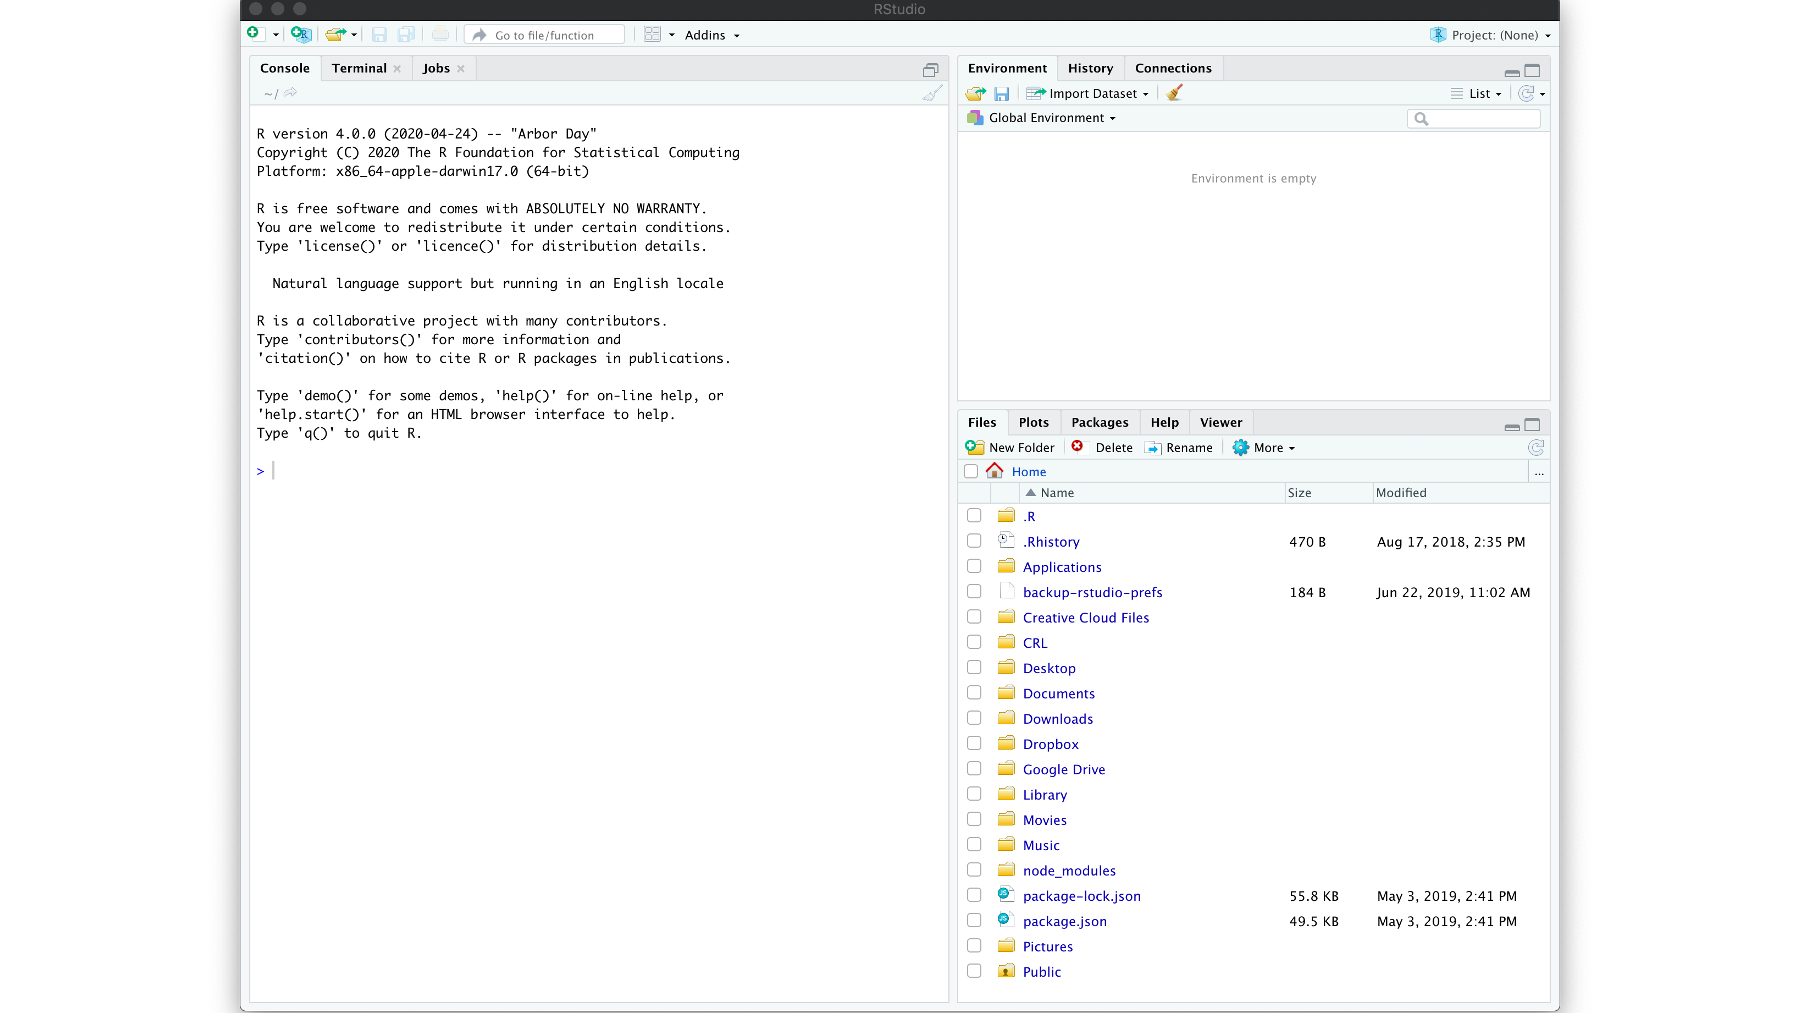
\includegraphics{chapters/installing_r_and_rstudio/mac_view_rstudio.png}

\section{Download and install on a
PC}\label{download-and-install-on-a-pc}

\textbf{Step 2:} Navigate to the Comprehensive R Archive Network (CRAN),
which is located at https://cran.r-project.org/.

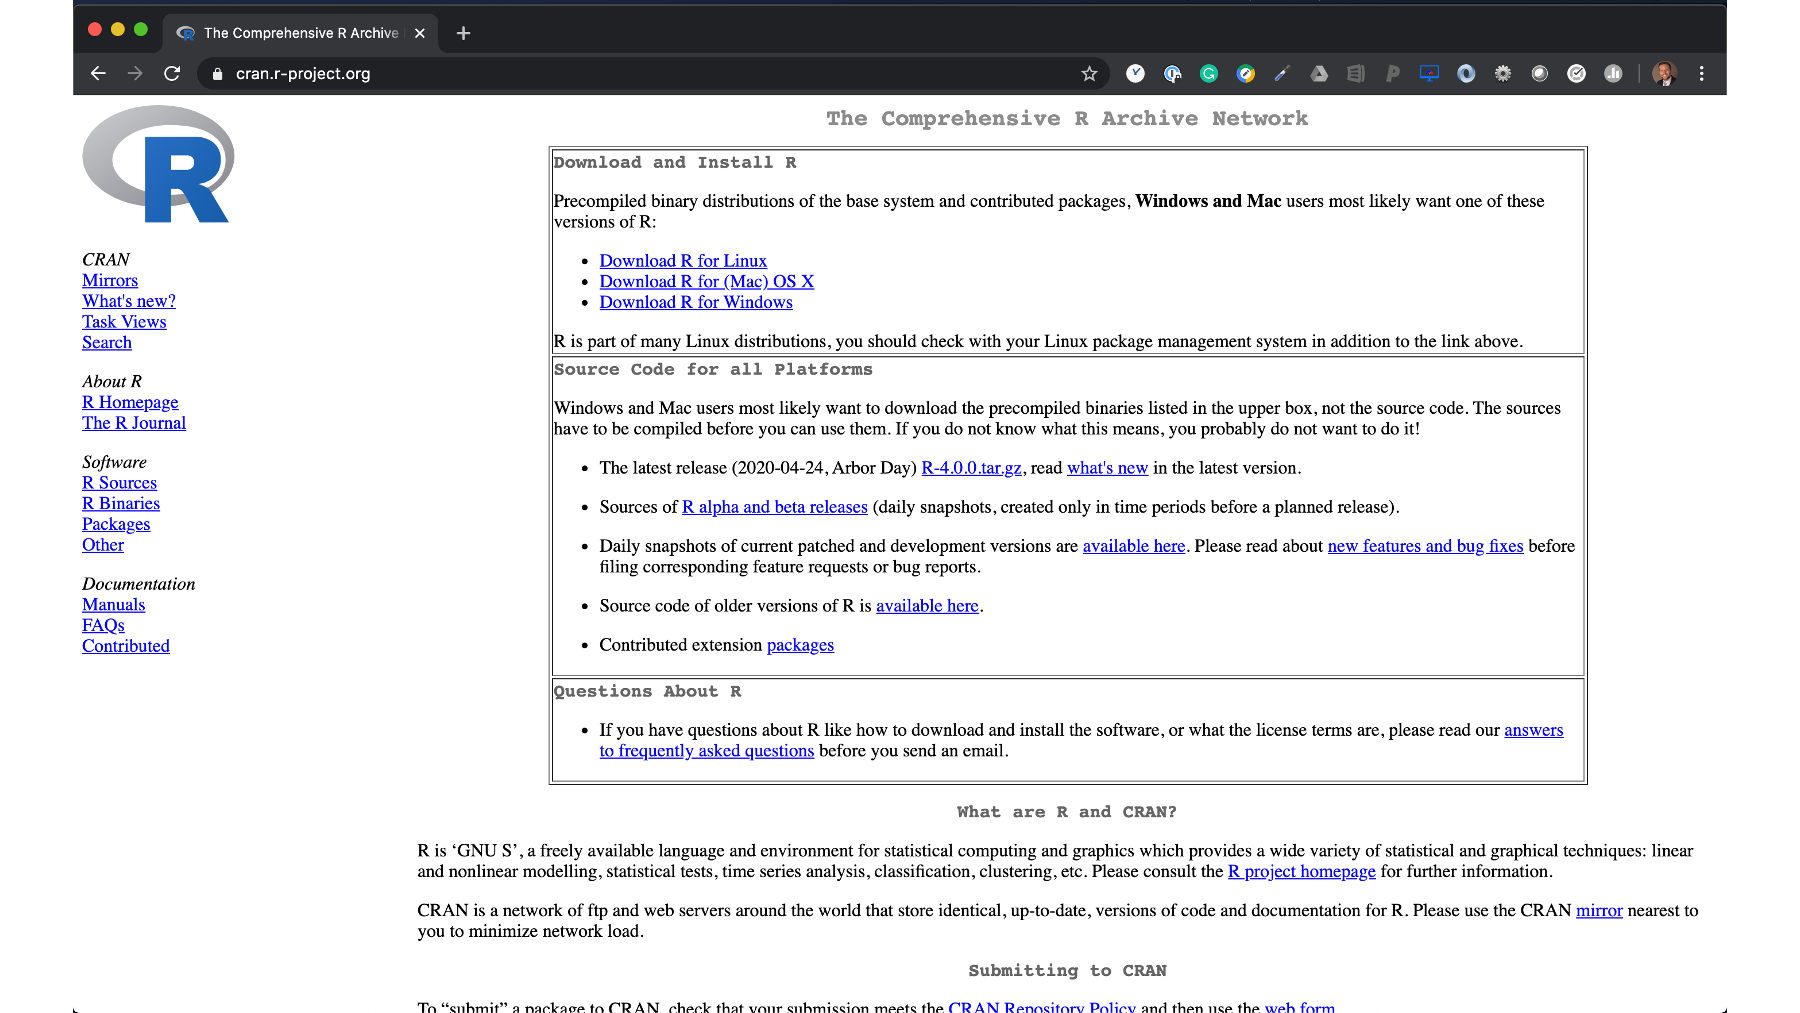
\includegraphics{chapters/installing_r_and_rstudio/pc_cran.png}

\textbf{Step 3:} Click on Download R for Windows.

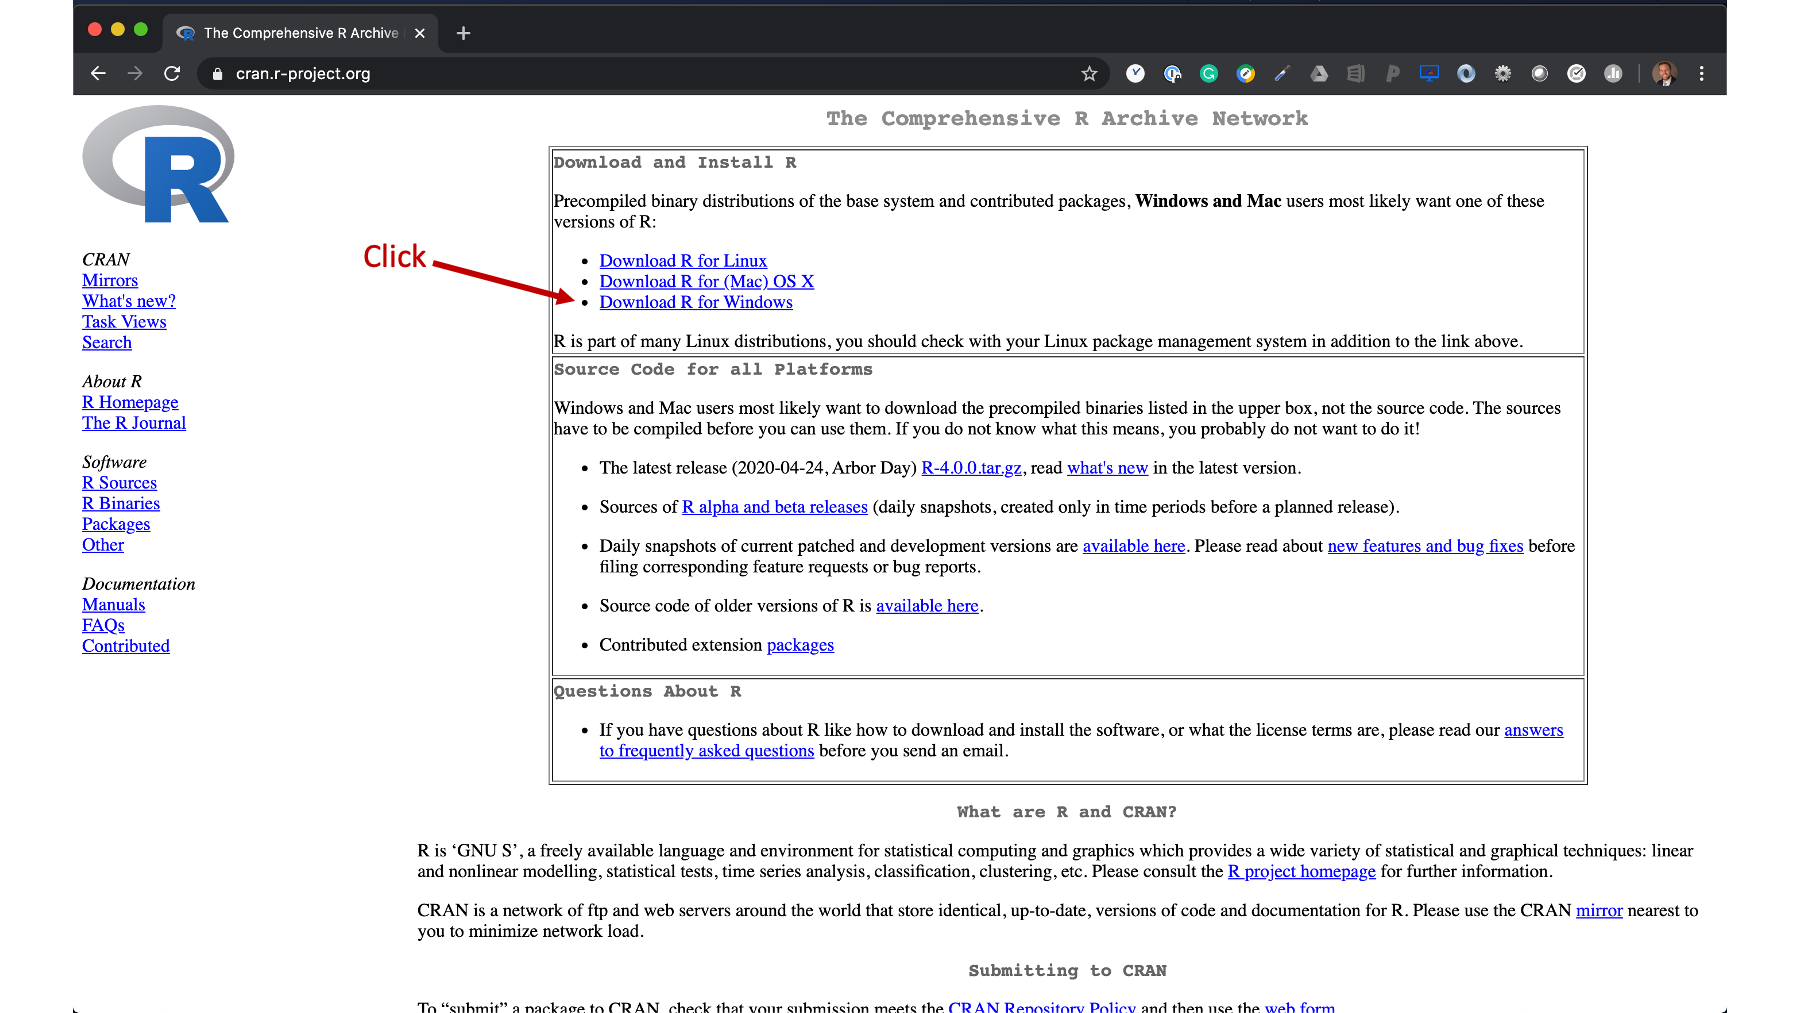
\includegraphics{chapters/installing_r_and_rstudio/pc_download_r1.png}

\textbf{Step 4:} Click on the base link.

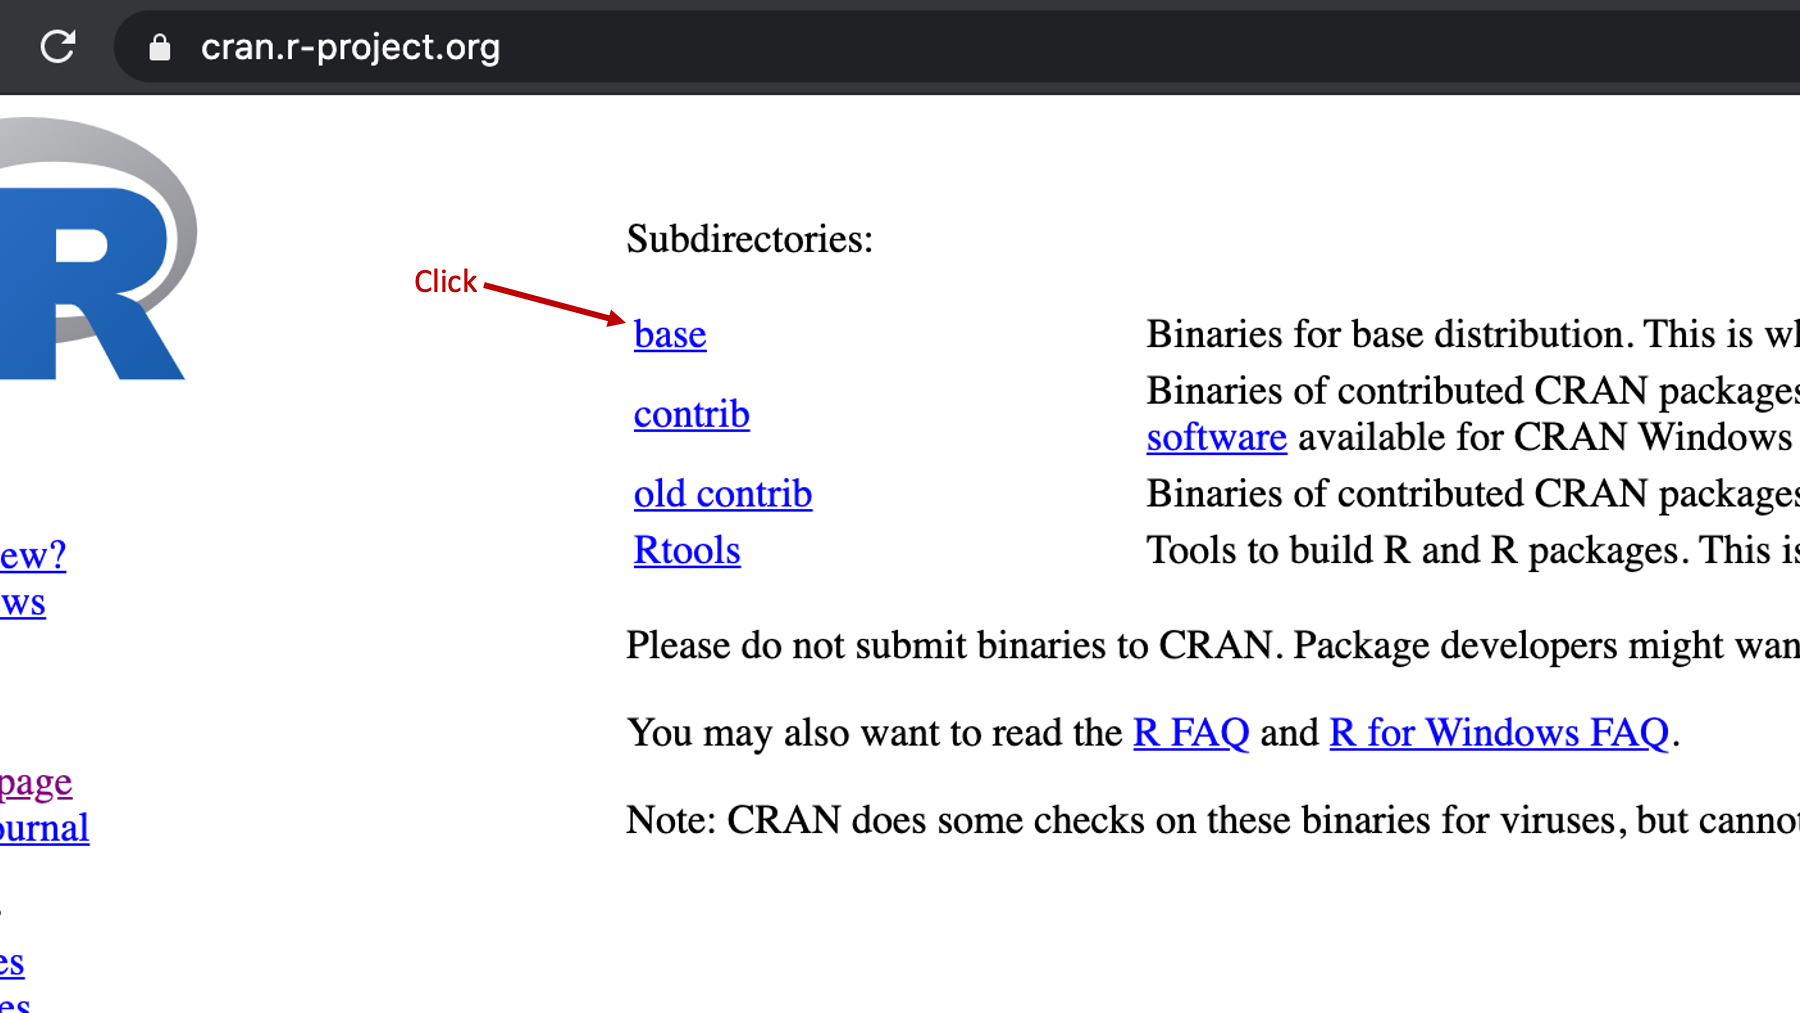
\includegraphics{chapters/installing_r_and_rstudio/pc_download_r2.png}

\textbf{Step 5:} Click on the link for the latest version of R. As you
are reading this, the newest version may be different than the version
you see in this picture, but the location of the newest version should
be roughly the same. After clicking, R should start to download to your
computer.

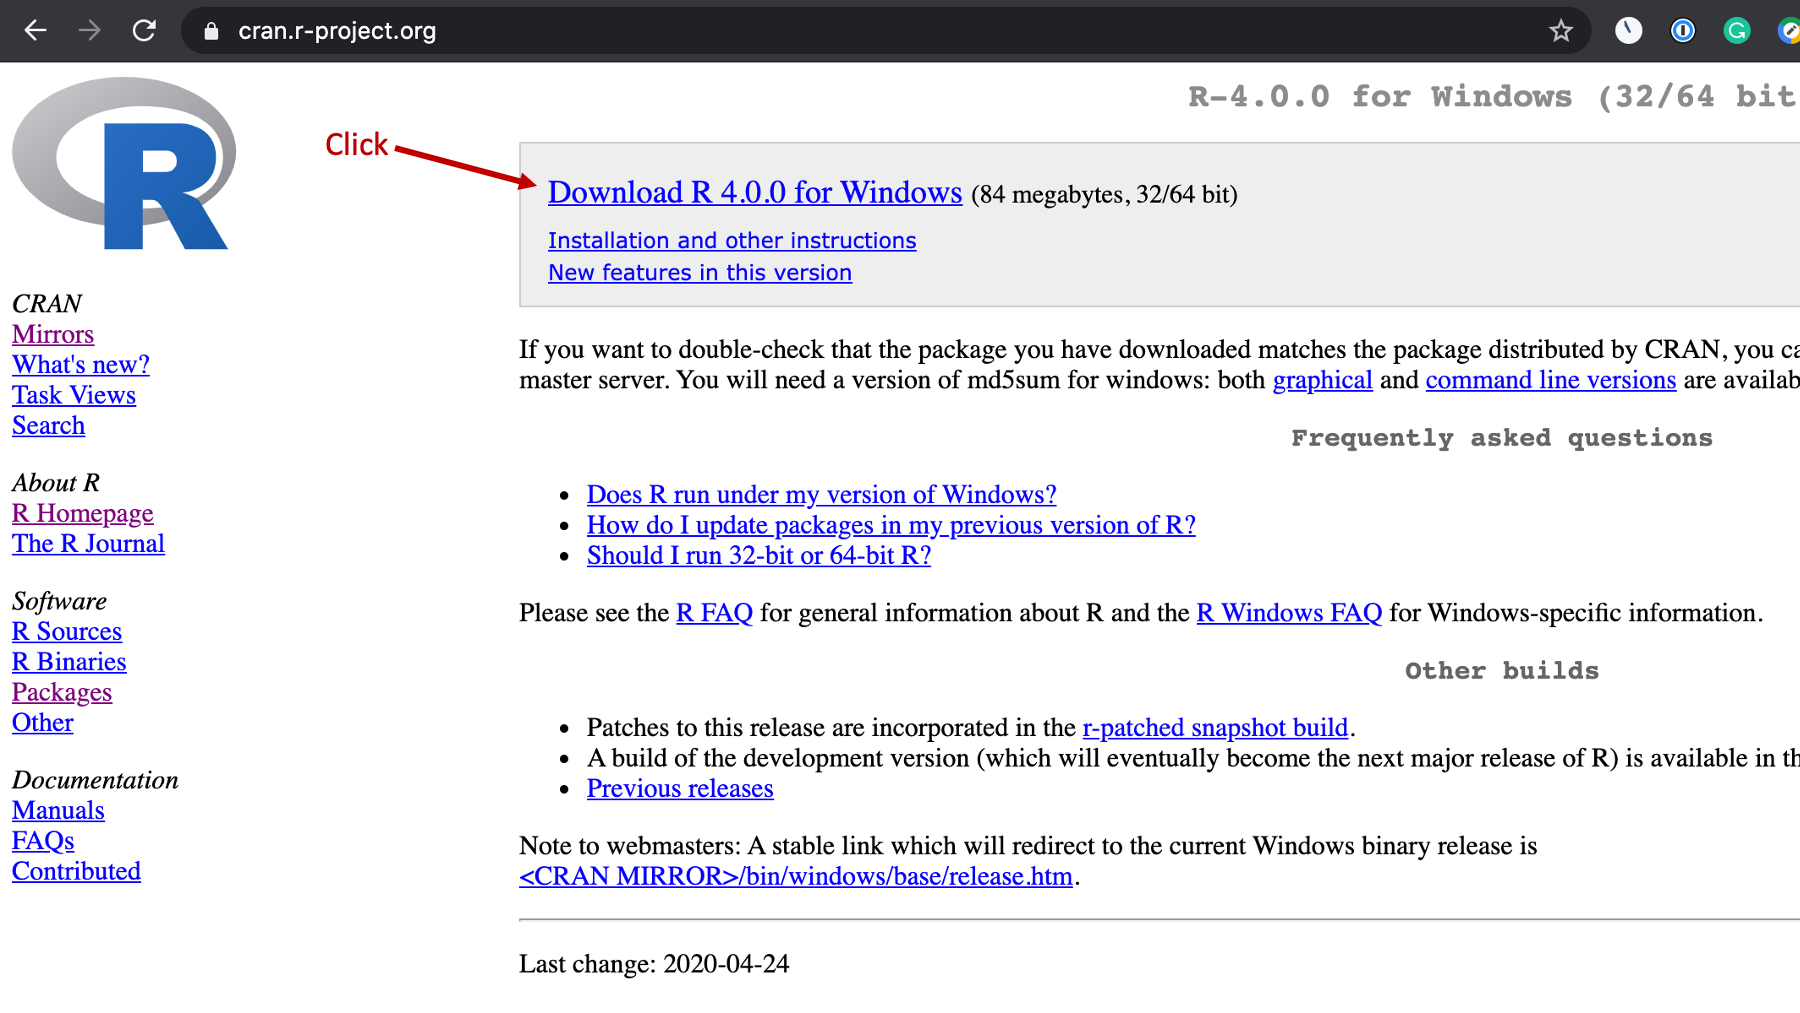
\includegraphics{chapters/installing_r_and_rstudio/pc_download_r3.png}

\textbf{Step 6:} Locate the installation file you just downloaded and
double click it. Unless you've changed your download settings, this file
will probably be in your downloads folder. That is the default location
for most web browsers.

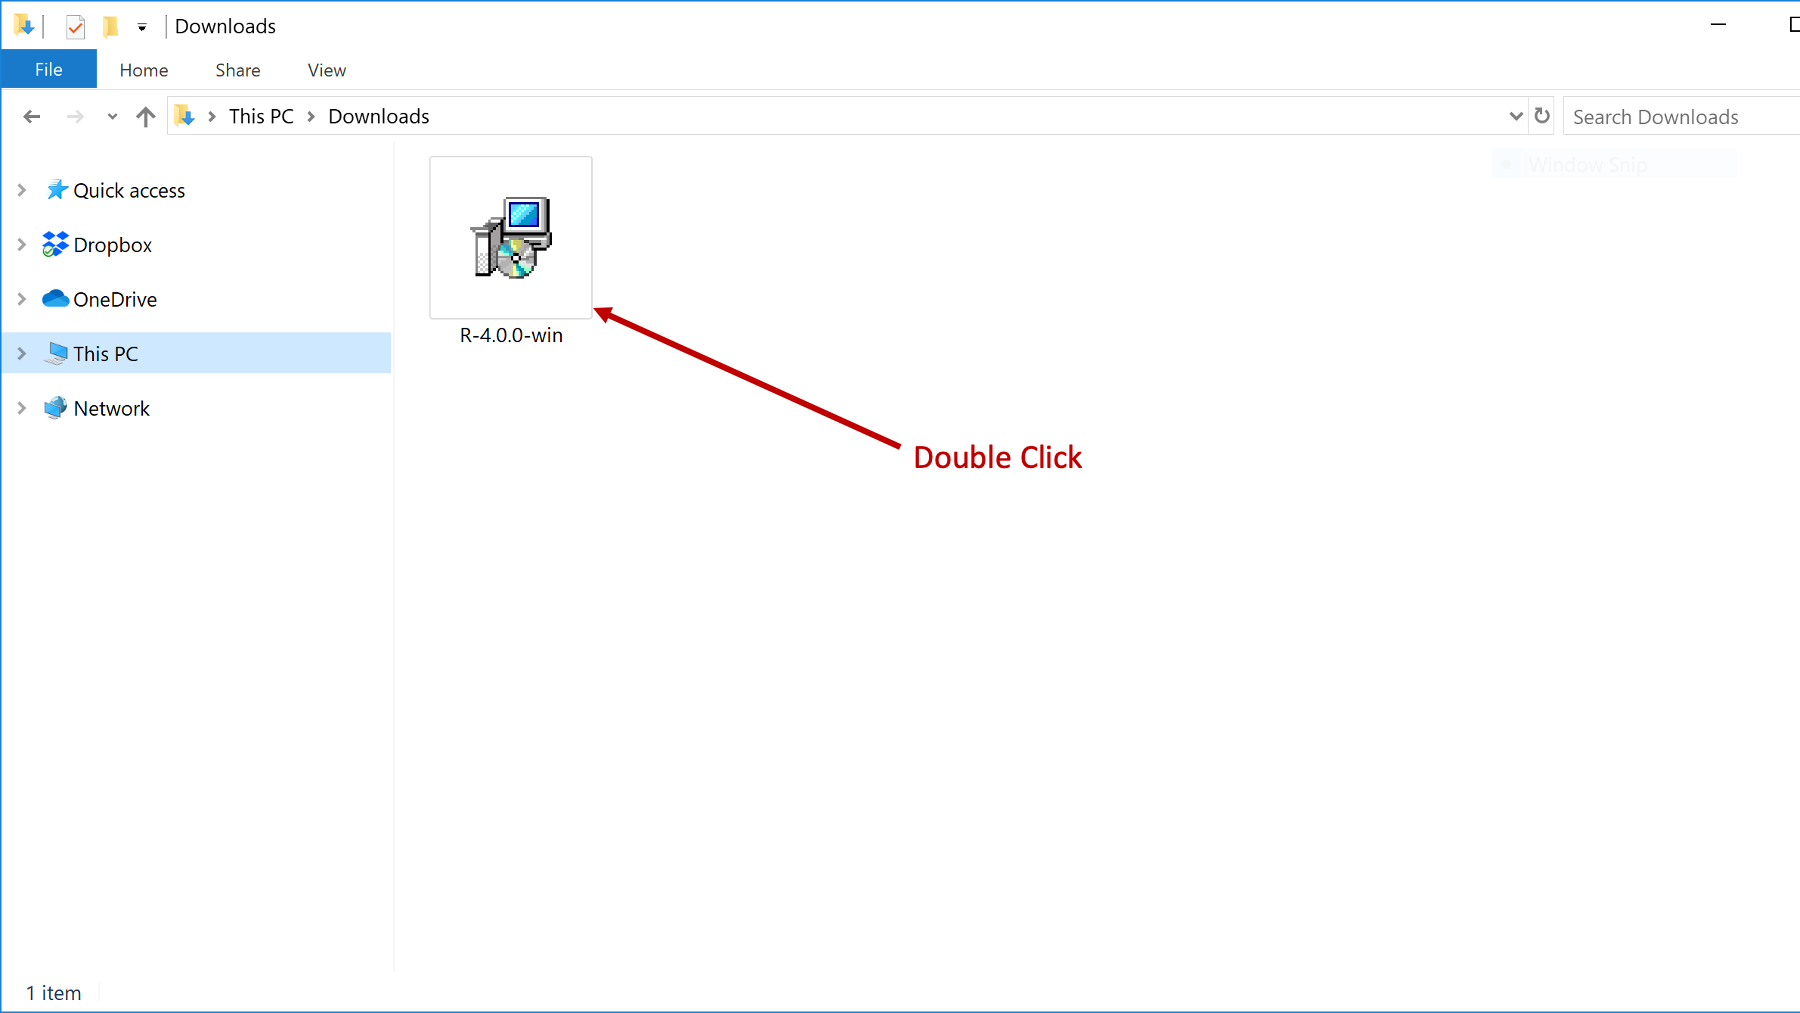
\includegraphics{chapters/installing_r_and_rstudio/pc_install_r1.png}

\textbf{Step 7:} A dialogue box will open that asks you to make some
decisions about how and where you want to install R on your computer. We
typically just click ``Next'' at every step without changing any of the
default options.

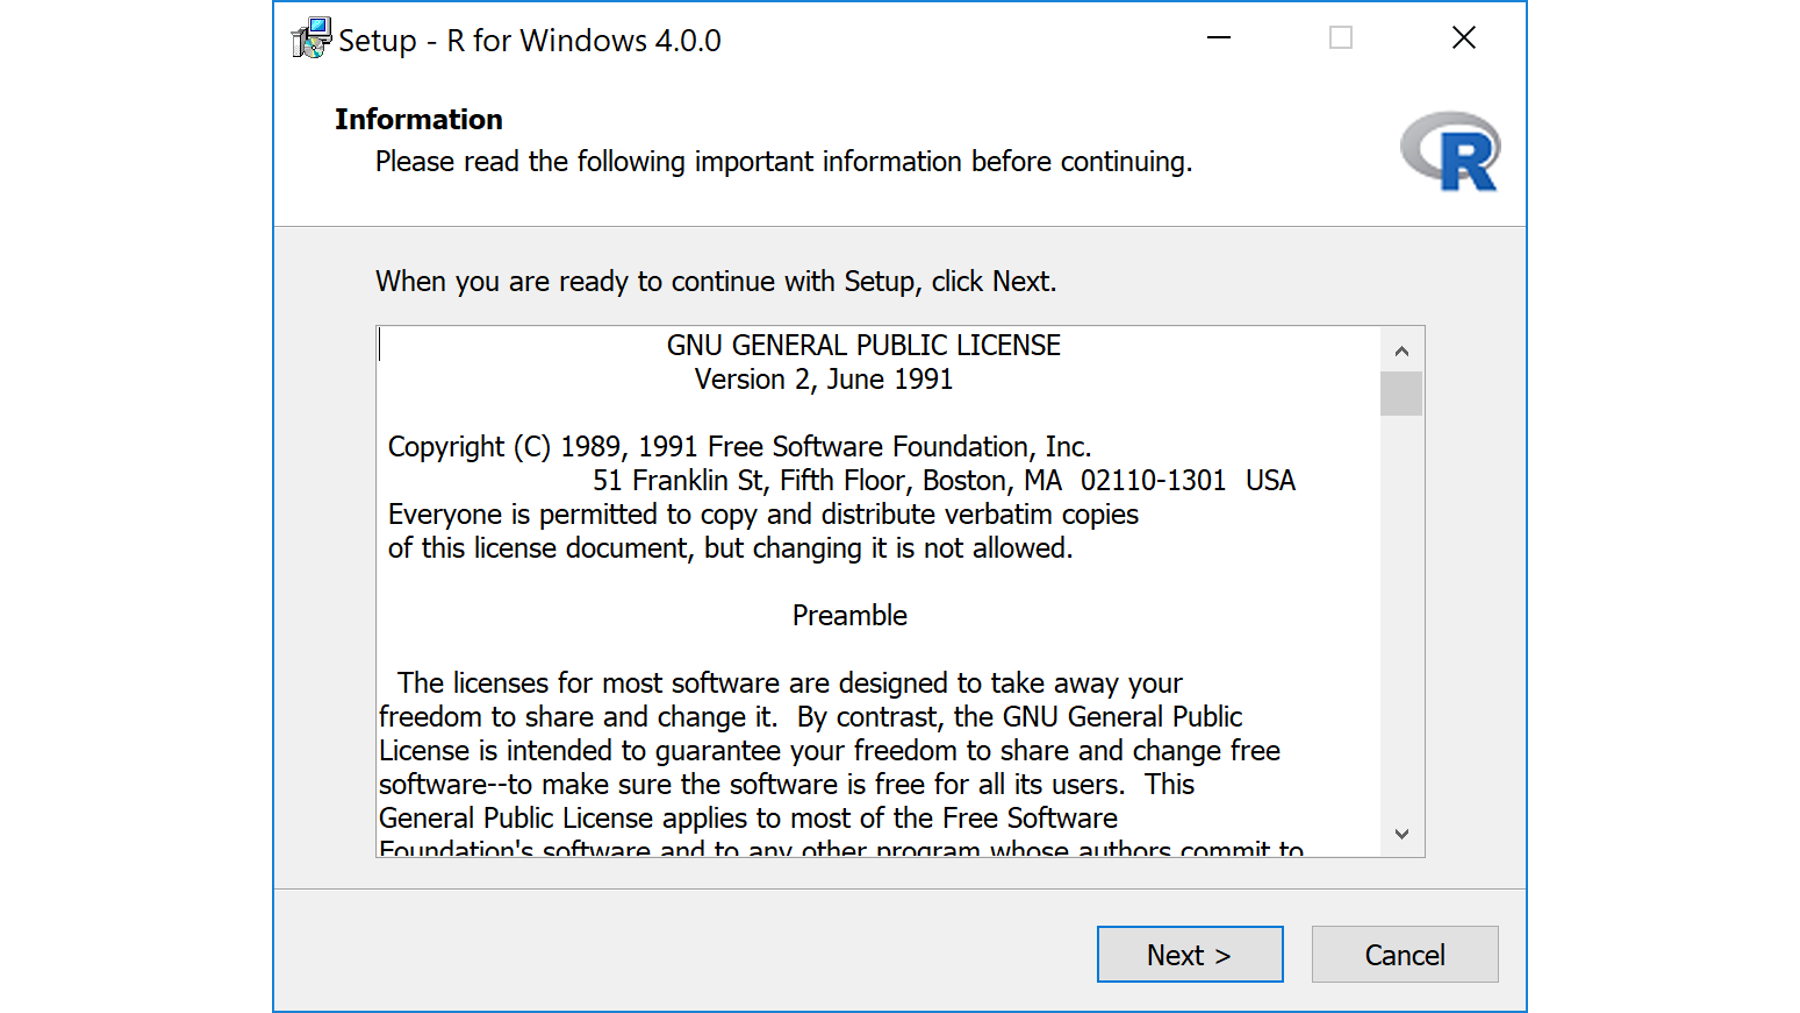
\includegraphics{chapters/installing_r_and_rstudio/pc_install_r2.png}

If R installed properly, you should now see it in the Windows start
menu.

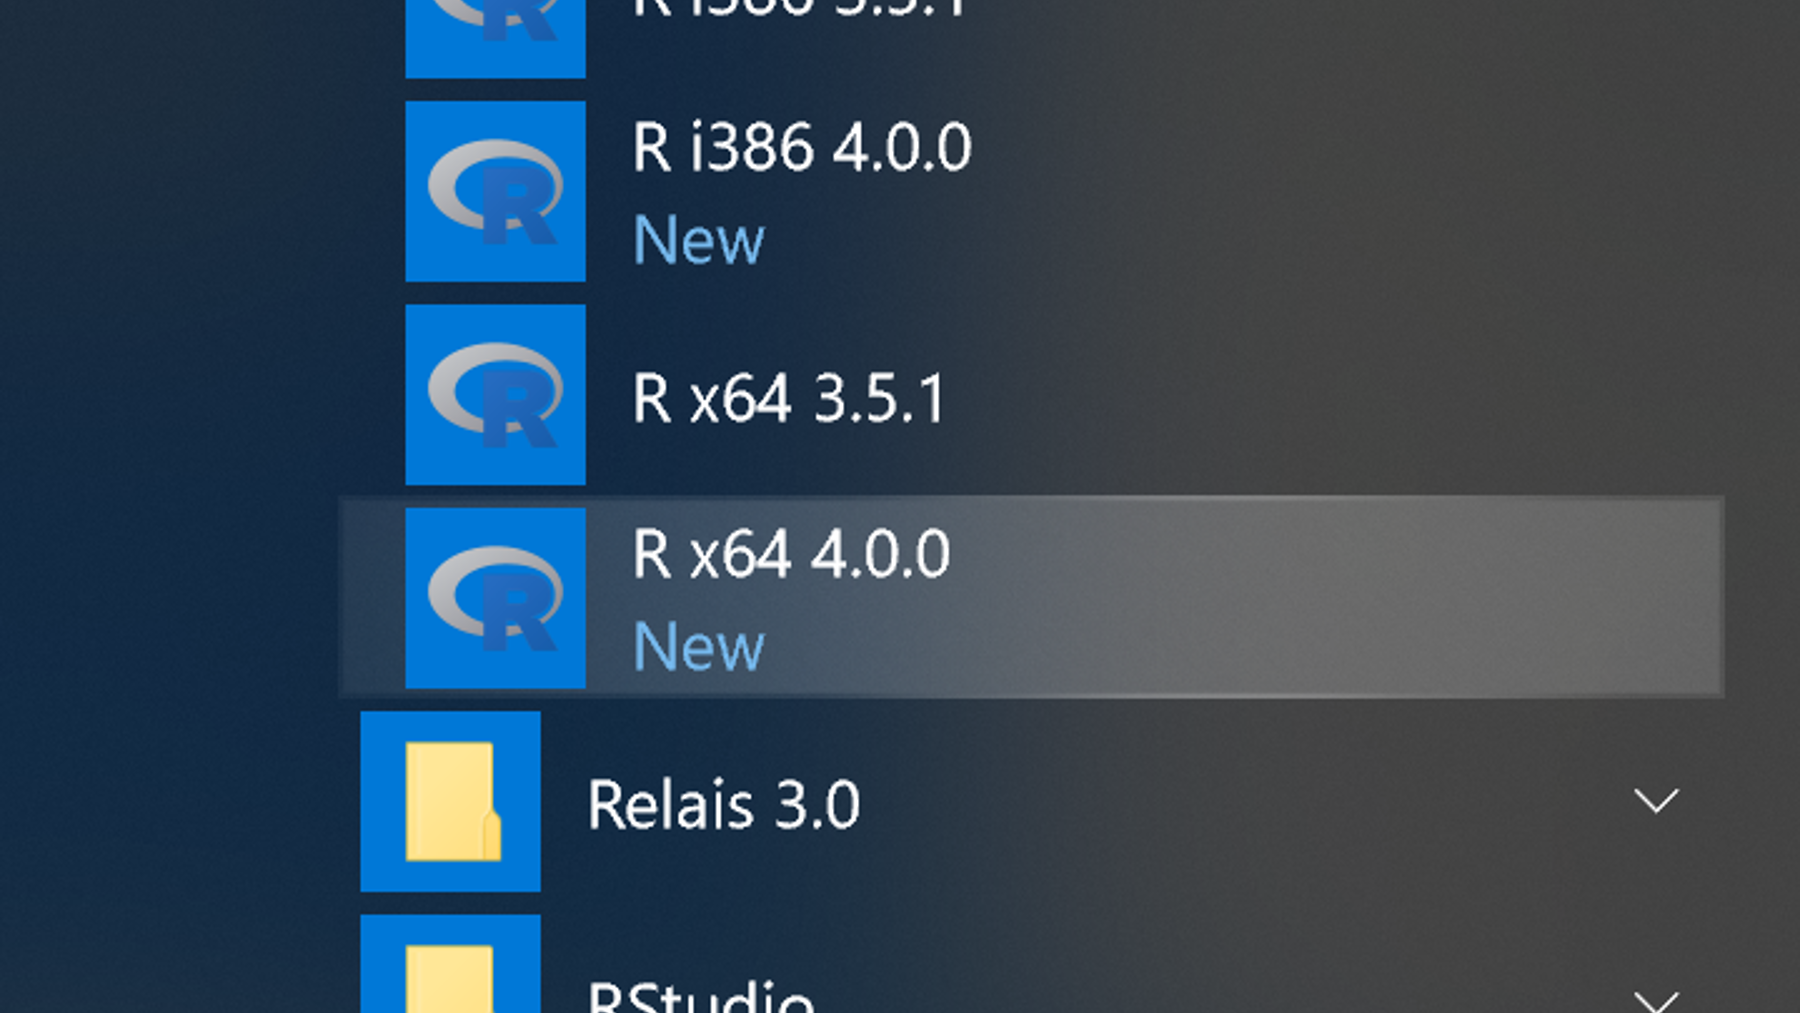
\includegraphics{chapters/installing_r_and_rstudio/pc_view_r.png}

\textbf{Step 8:} Now, we need to install the RStudio IDE. To do this,
navigate to the RStudio desktop download website, which is located at
https://posit.co/download/rstudio-desktop/. On that page, click the
button to download the latest version of RStudio for your computer. Note
that the website may look different that what you see in the screenshot
below because websites change over time.

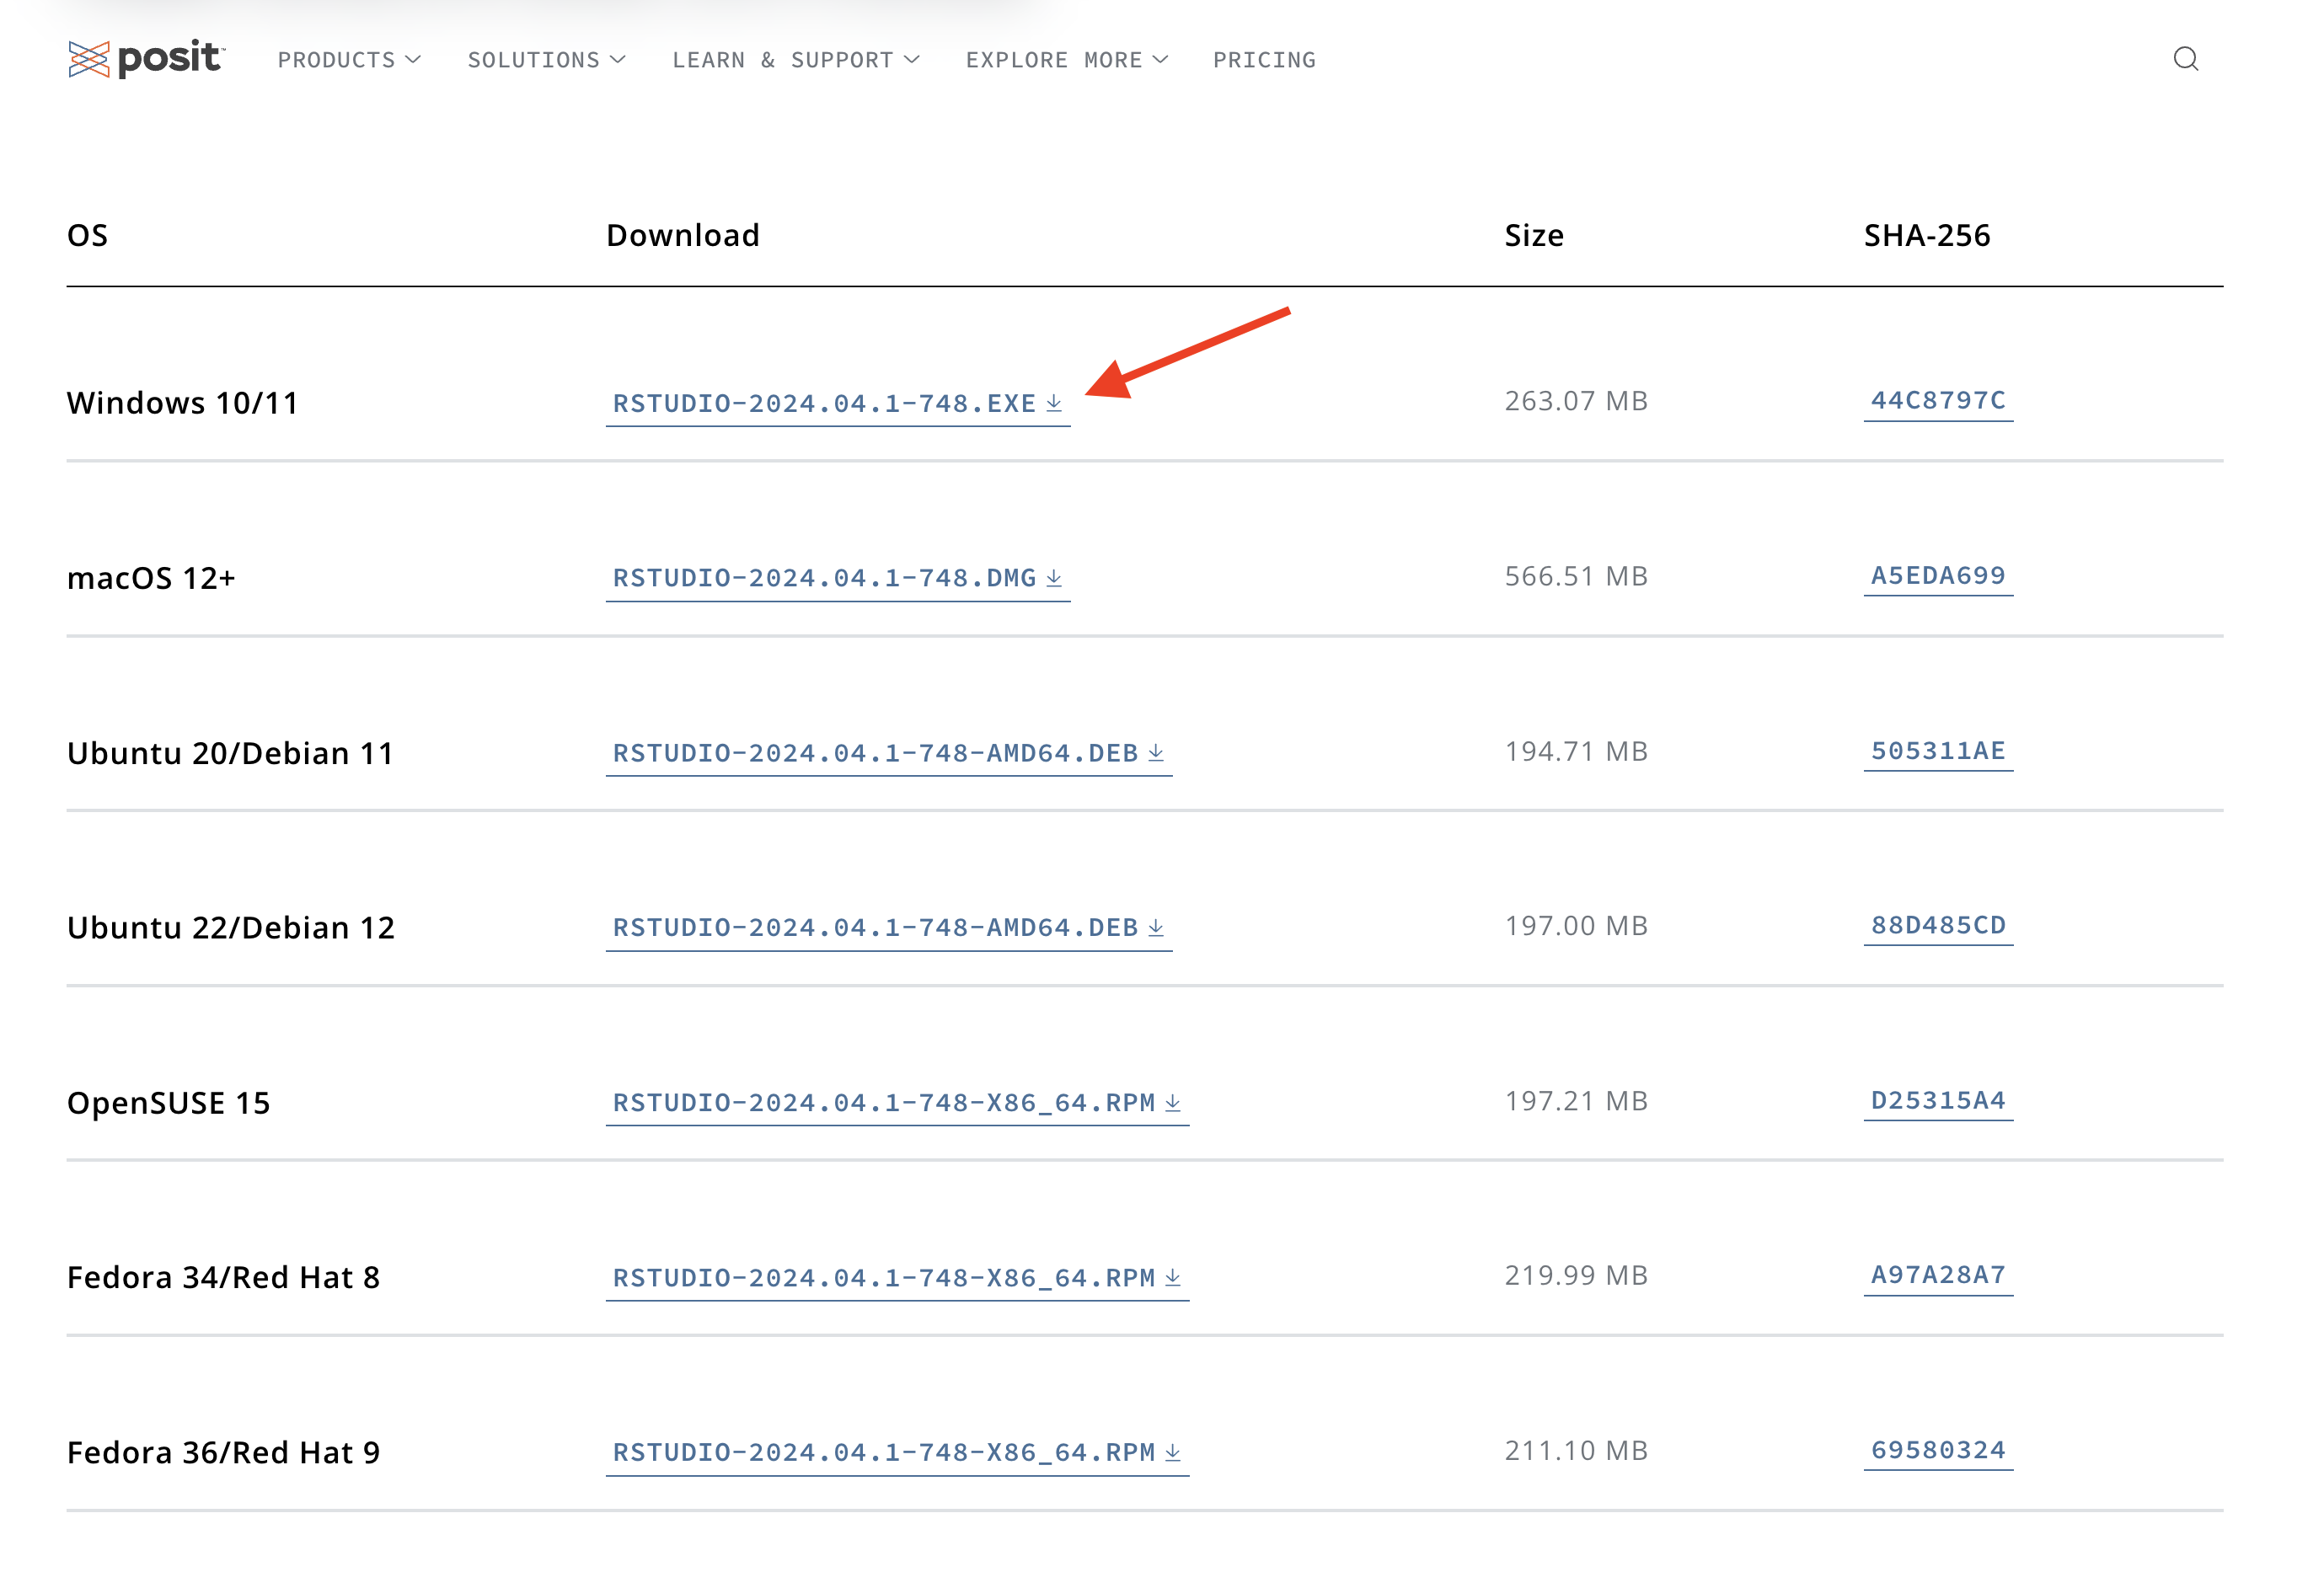
\includegraphics{chapters/installing_r_and_rstudio/pc_download_rstudio1.png}

\textbf{Step 9:} Again, locate the installation file you just downloaded
and double click it. Unless you've changed your download settings, this
file should be in the same location as the R installation file you
already downloaded.

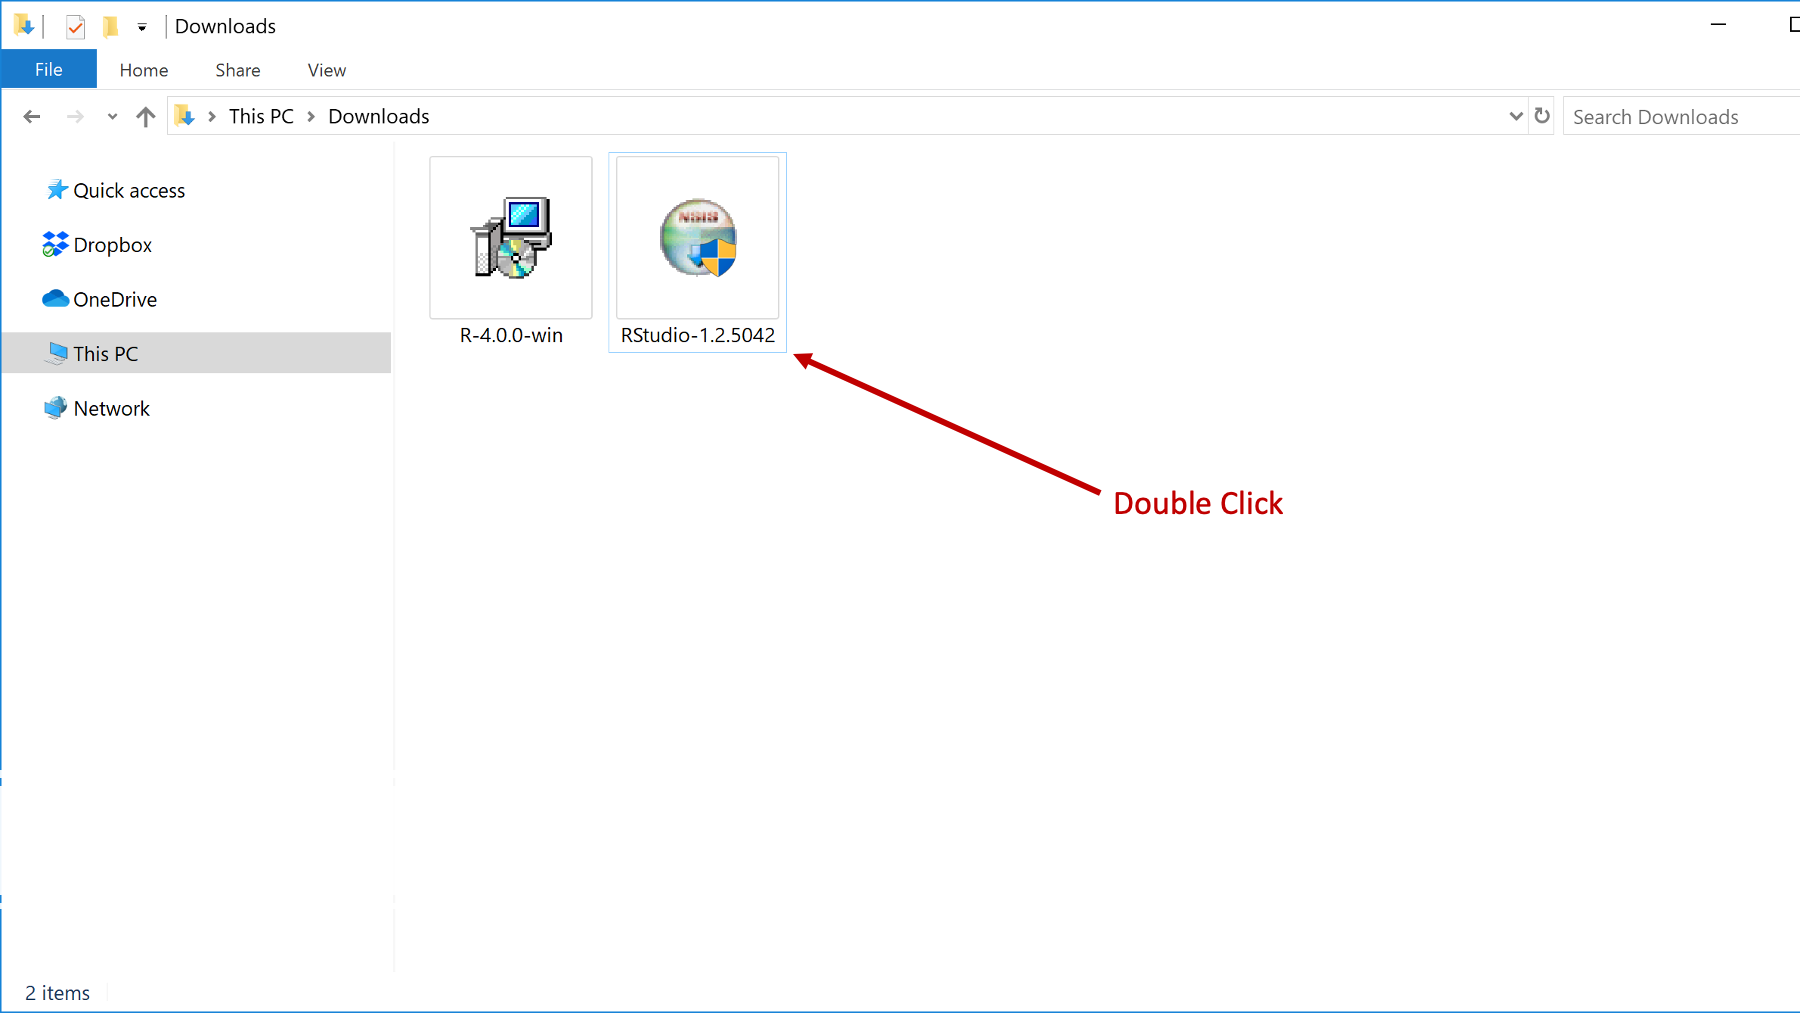
\includegraphics{chapters/installing_r_and_rstudio/pc_install_rstudio1.png}

\textbf{Step 10:} Another dialogue box will open and ask you to make
some decisions about how and where you want to install RStudio on your
computer. We typically just click ``Next'' at every step without
changing any of the default options.

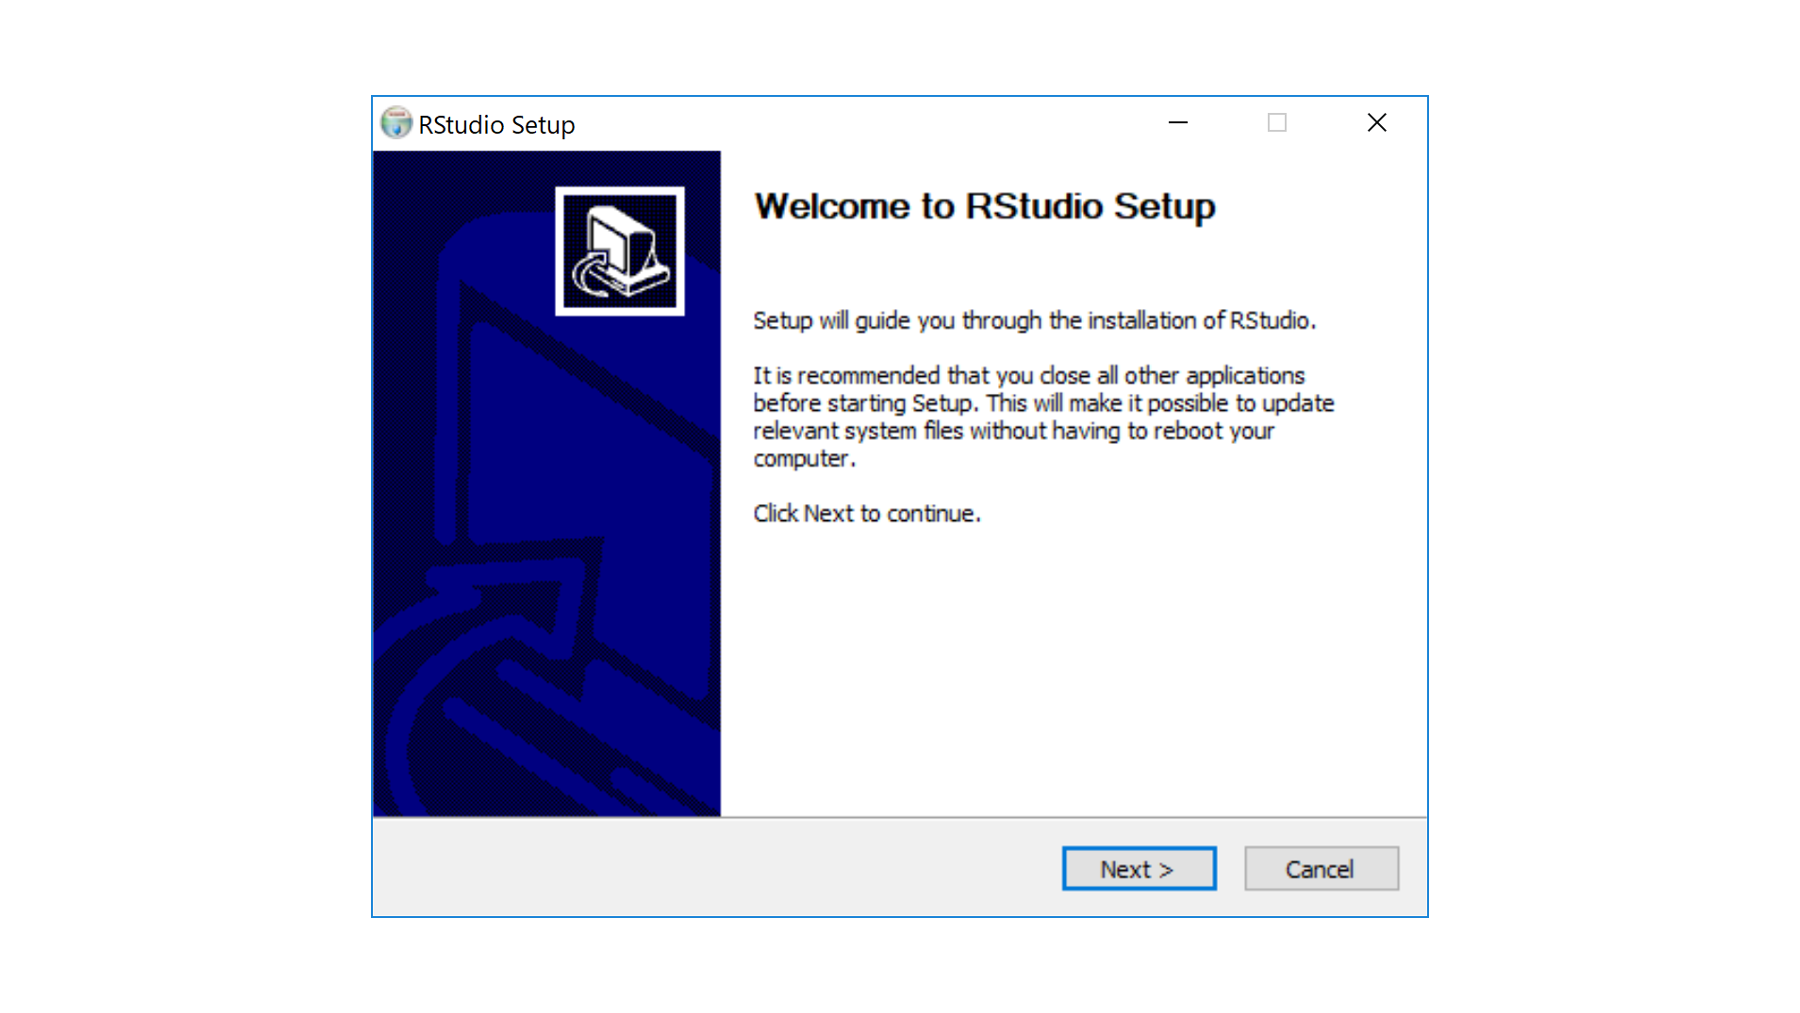
\includegraphics{chapters/installing_r_and_rstudio/pc_install_rstudio2.png}

When RStudio is finished installing, you should see RStudio in the
Windows start menu. Click the icon to open RStudio.

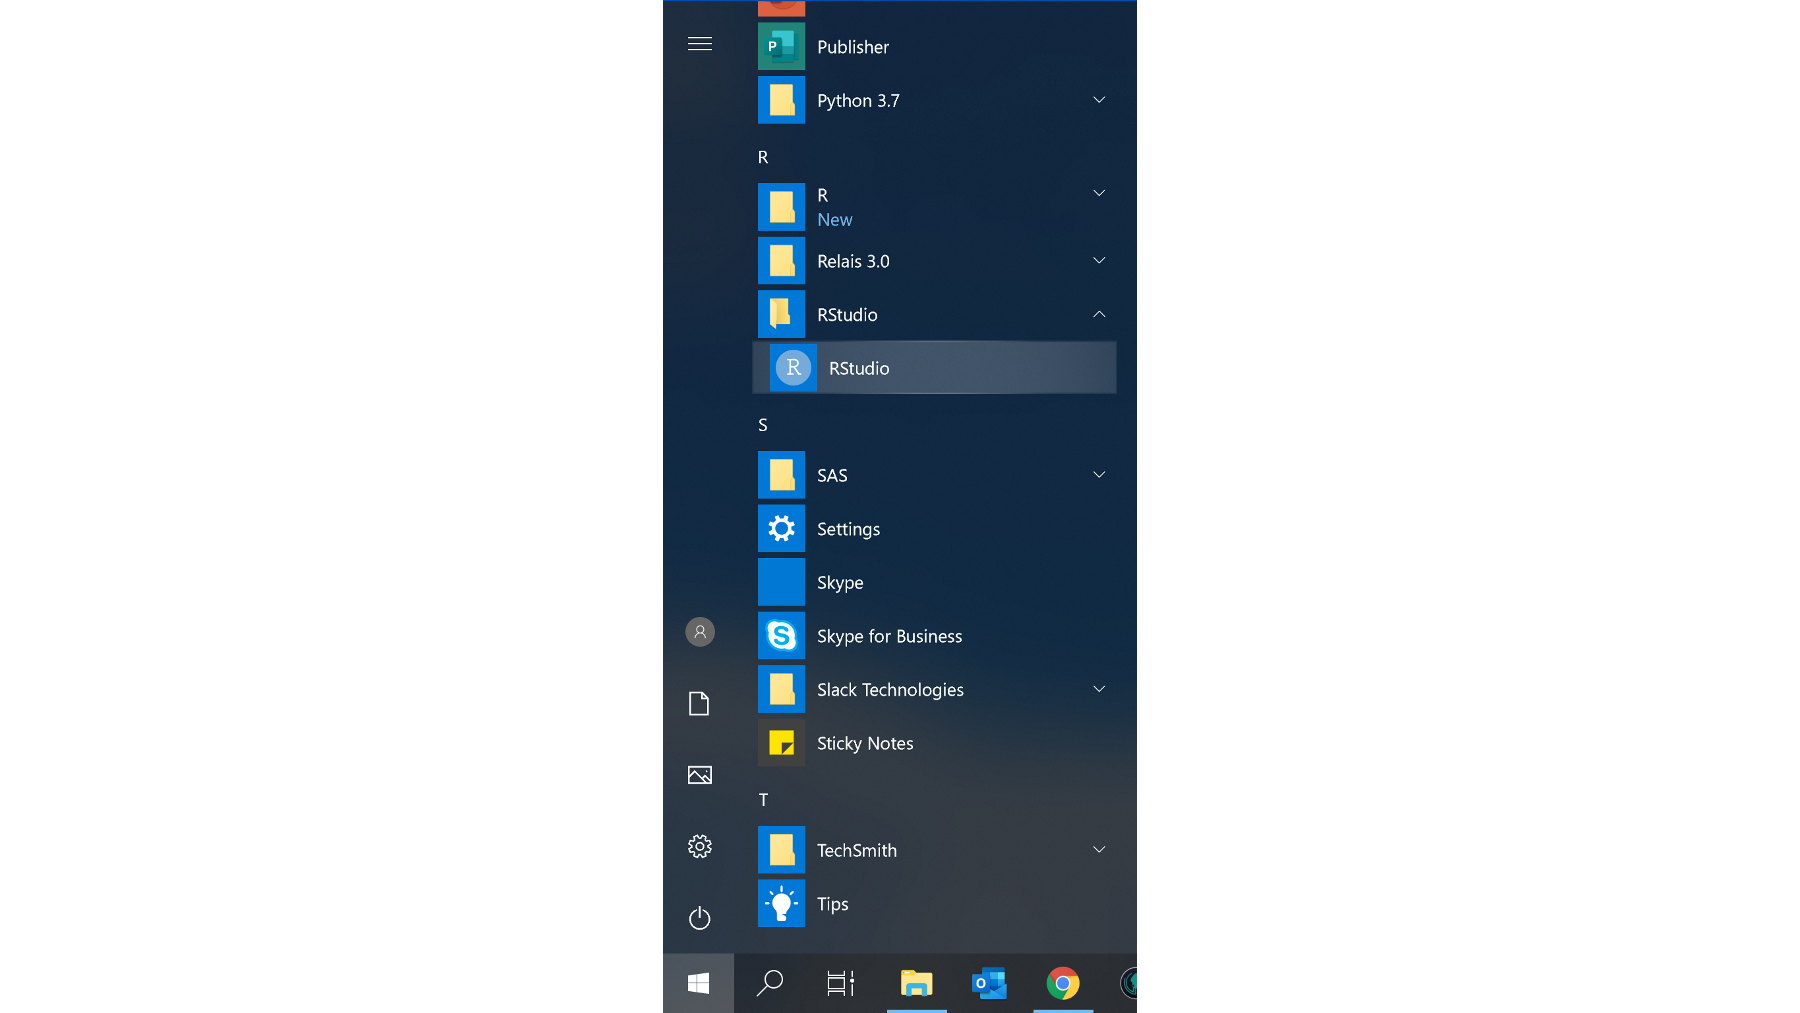
\includegraphics{chapters/installing_r_and_rstudio/pc_view_rstudio1.png}

The RStudio IDE should open and look something like the window you see
here. If so, you are good to go! 🎉

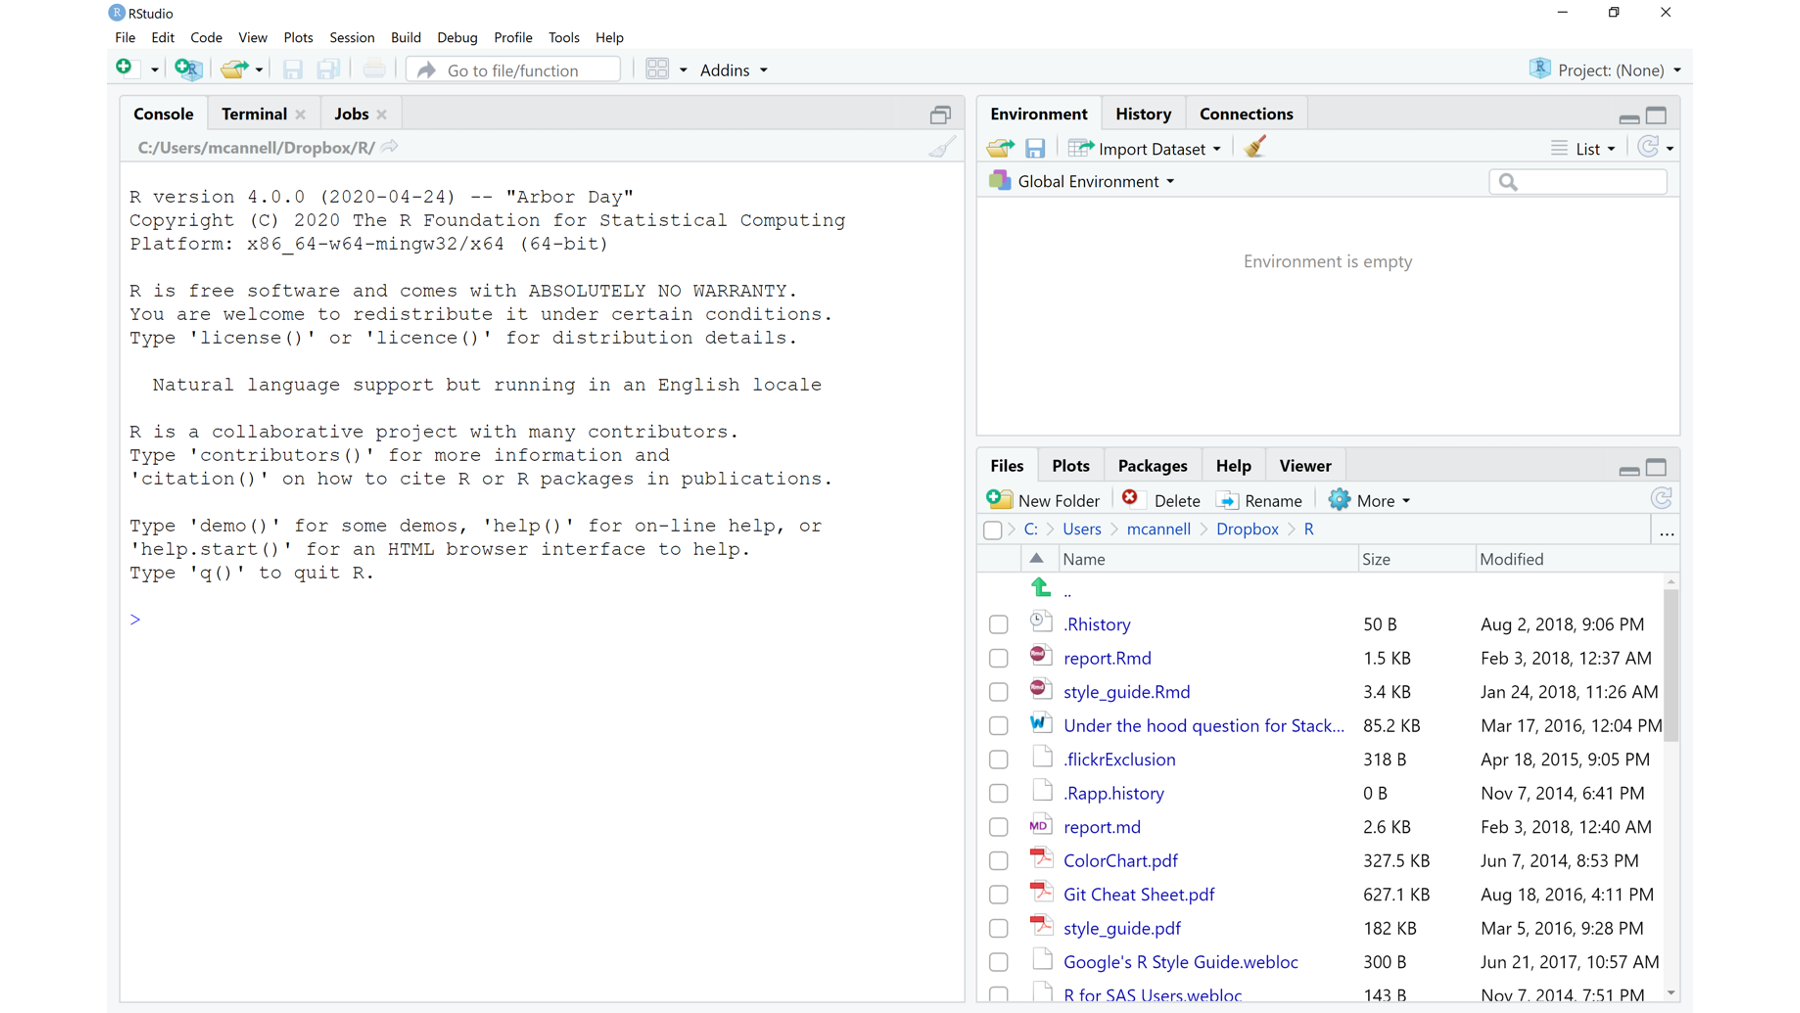
\includegraphics{chapters/installing_r_and_rstudio/pc_view_rstudio2.png}

\chapter{What is R?}\label{what-is-r}

At this point in the book, you should have installed R and RStudio on
your computer, but you may be thinking to yourself, ``I don't even know
what R is.'' Well, in this chapter you'll find out. We'll start with an
overview of the R language, and then briefly touch on its capabilities
and uses. You'll also see a complete R program and some complete
documents generated by R programs. In this book you'll learn how to
create similar programs and documents, and by the end of the book you'll
be able to write your own R programs and present your results in the
form of an issue brief written for general audiences who may or may not
have public health expertise. But, before we discuss R let's discuss
something even more basic -- data. Here's a question for you: What is
data?

\section{What is data?}\label{what-is-data}

Data is information about objects (e.g., people, places, schools) and
observable phenomenon (e.g., weather, temperatures, and disease
symptoms) that is recorded and stored somehow as a collection of
symbols, numbers, and letters. So, data is just information that has
been ``written'' down.

Here we have a table, which is a common way of organizing data. In R, we
will typically refer to these tables as \textbf{data frames}.

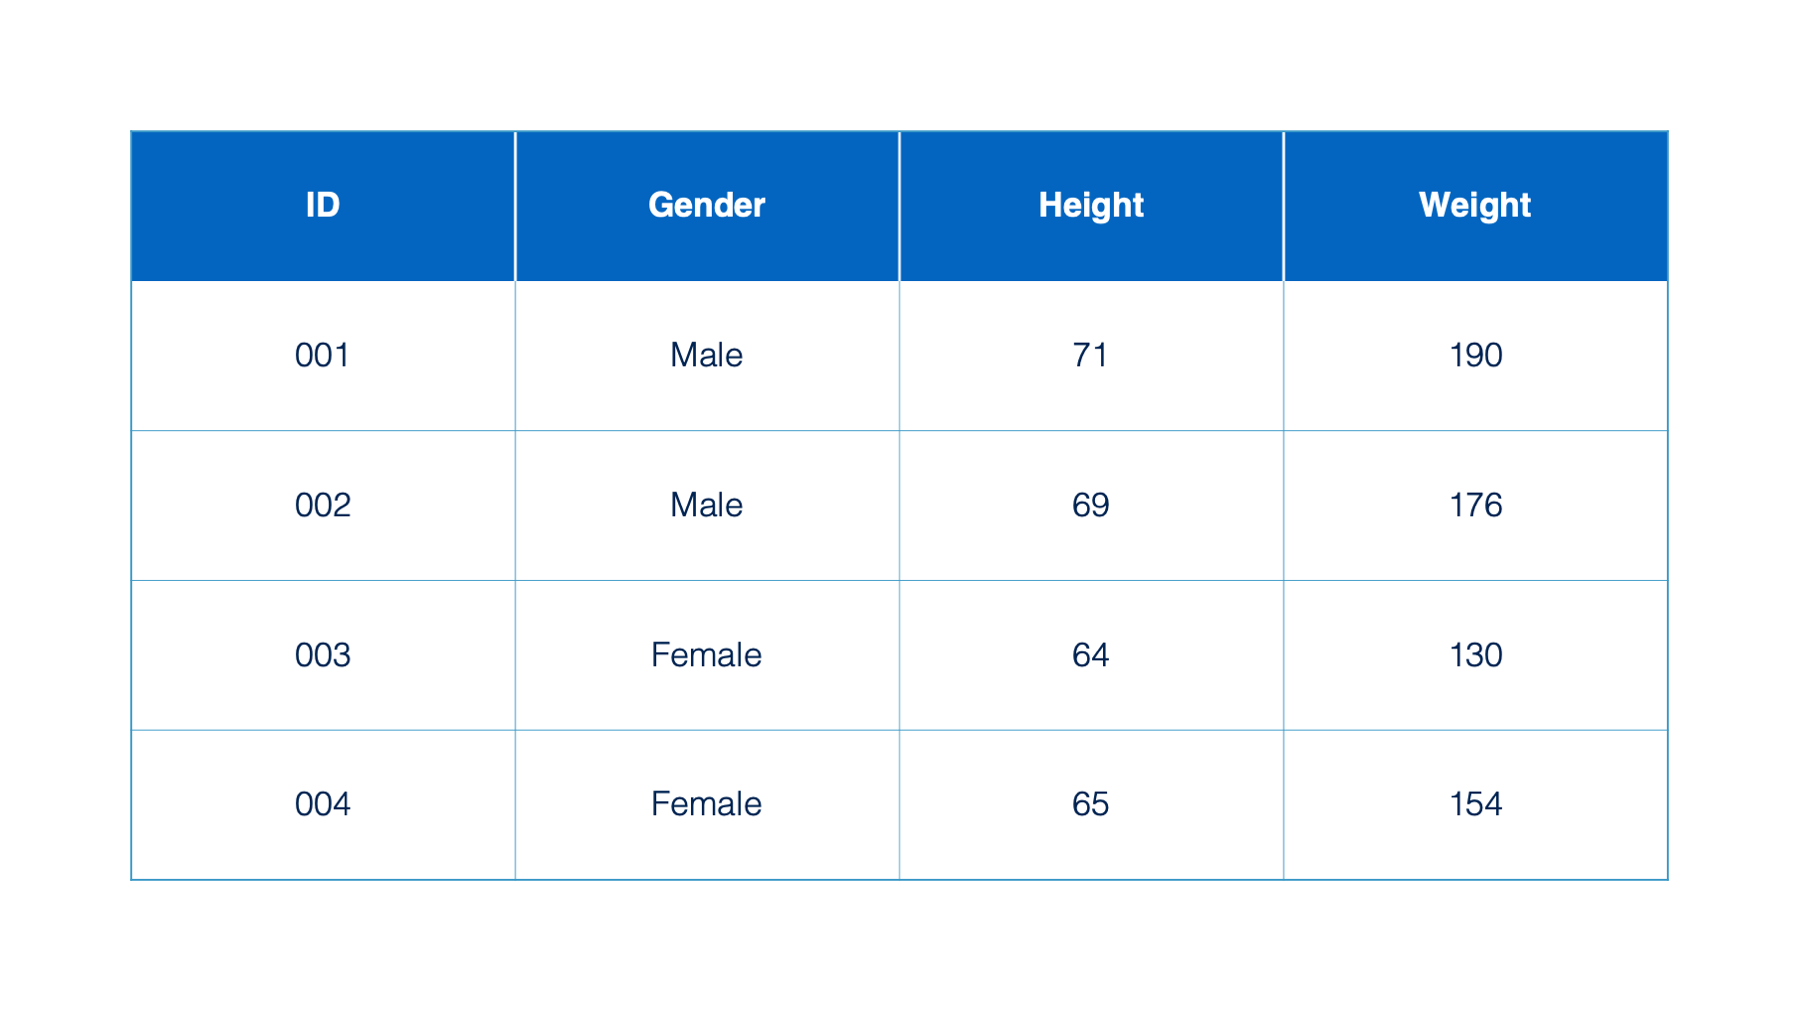
\includegraphics{chapters/what_is_r/table.png}

Each box in a data frame is called a \textbf{cell}.

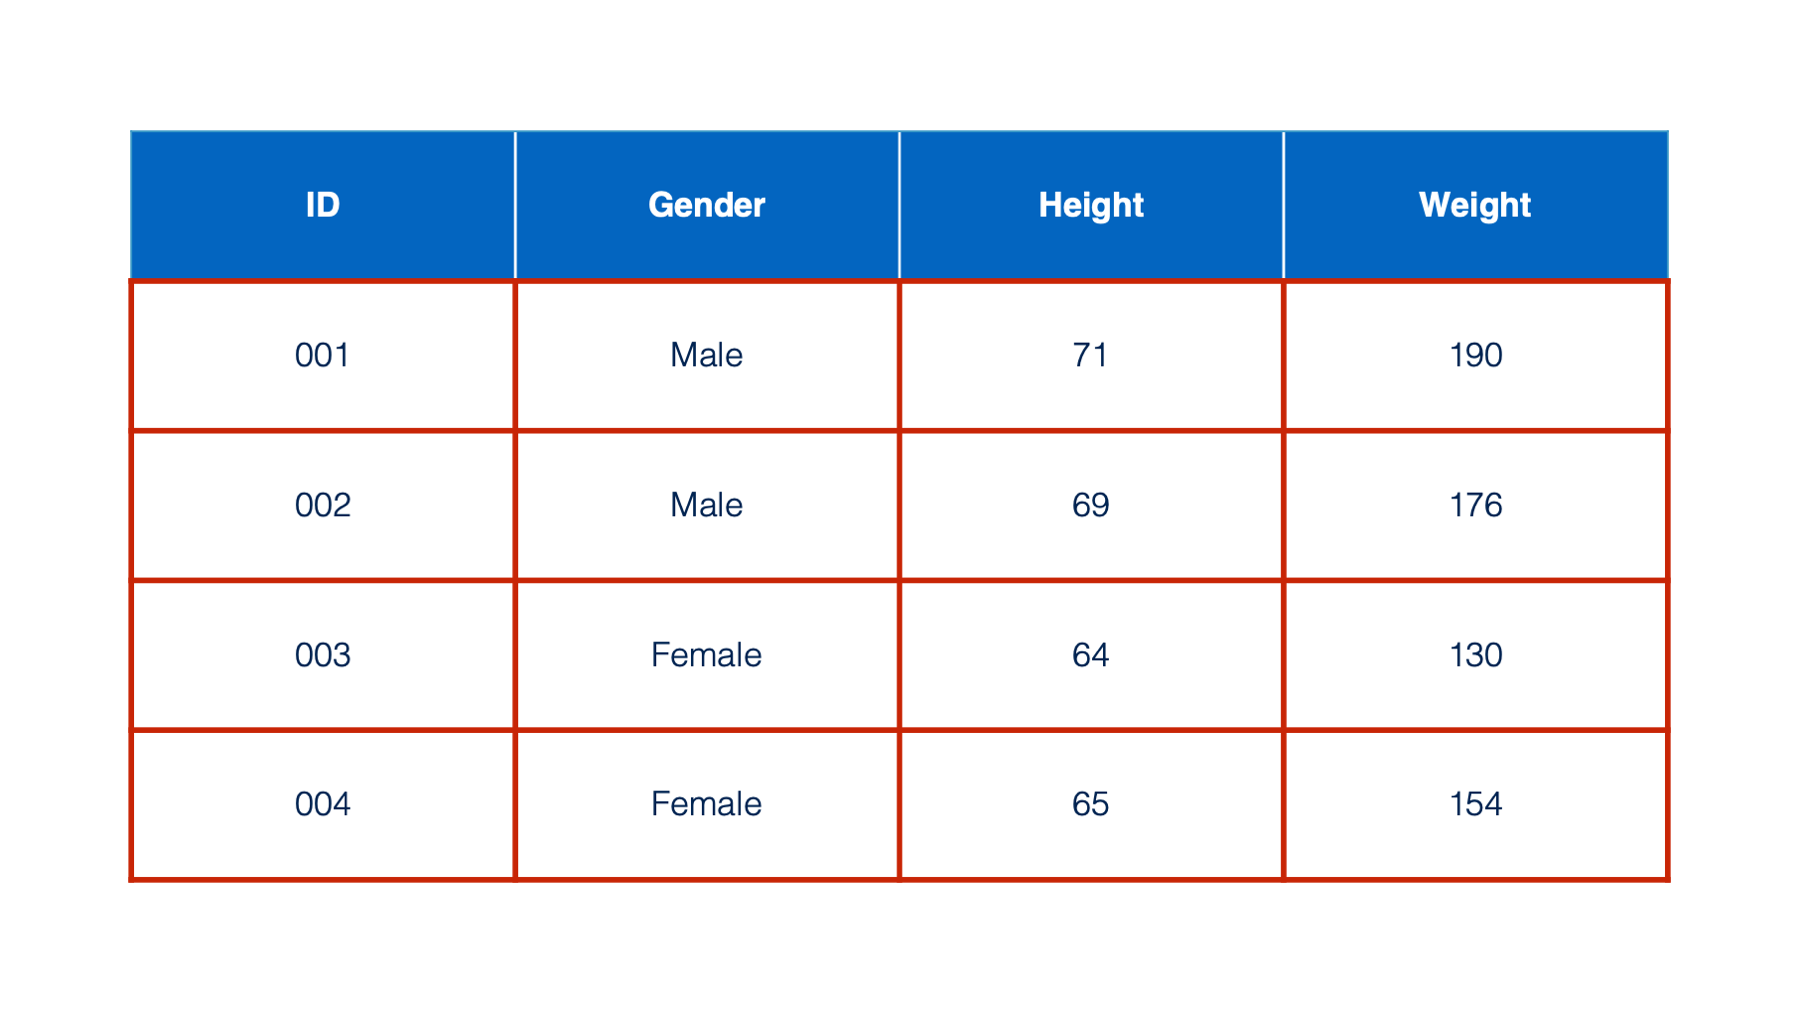
\includegraphics{chapters/what_is_r/table_cells.png}

Moving from left to right across the data frame are \textbf{columns}.
Columns are also sometimes referred to as \textbf{variables}. In this
book, we will often use the terms columns and variables interchangeably.
Each column in a data frame has one, and only one, type. For now, know
that the type tells us what kind of data is contained in a column and
what we can \emph{do} with that data. You may have already noticed that
3 of the columns in the table we've been looking at contain numbers and
1 of the columns contains words. These columns will have different types
in R and we can do different things with them based on their type. For
example, we could ask R to tell us what the average value of the numbers
in the height column are, but it wouldn't make sense to ask R to tell us
the average value of the words in the Gender column. We will talk more
about many of the different column types exist in R later in this book.

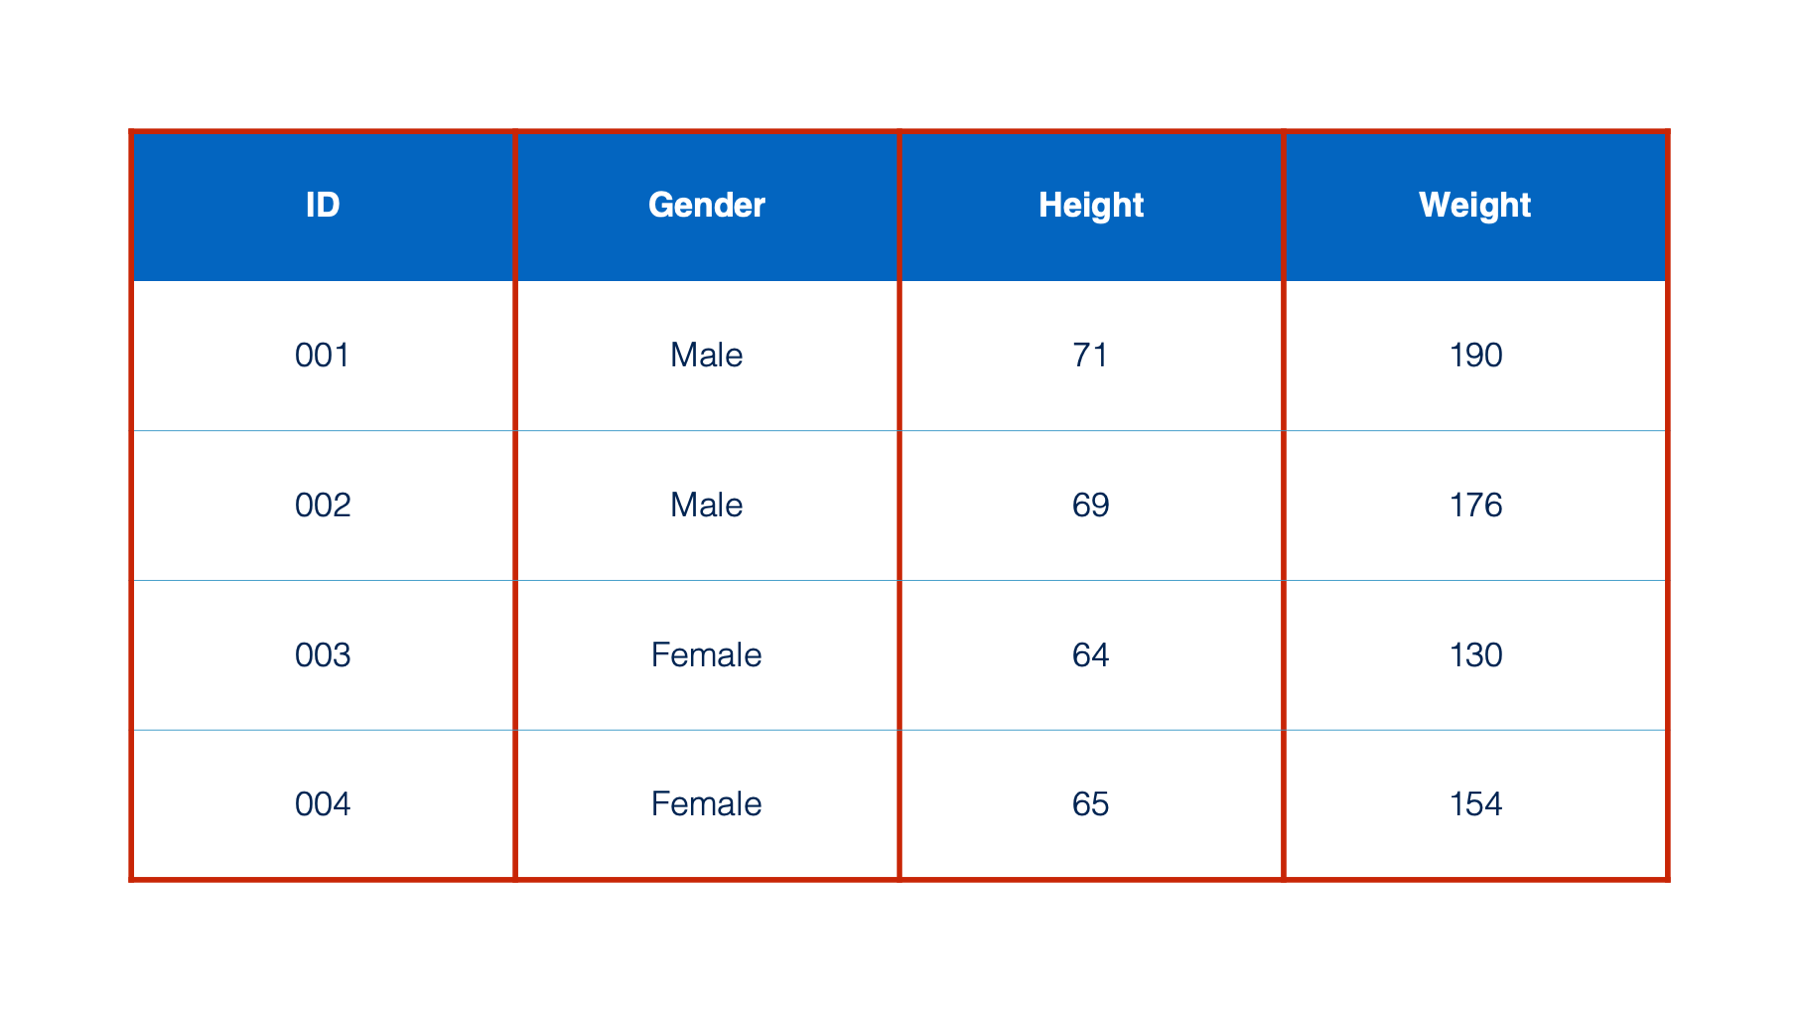
\includegraphics{chapters/what_is_r/table_columns.png}

The information contained in the first cell of each column is called the
\textbf{column name} (or variable) name.

R gives us a lot of flexibility in terms of what we can name our
columns, but there are a few rules.

\begin{enumerate}
\def\labelenumi{\arabic{enumi}.}
\tightlist
\item
  Column names can contain letters, numbers and the dot (.) or
  underscore (\_) characters.\\
\item
  Additionally, they can begin with a letter or a dot -- as long as the
  dot is not followed by a number. So, a name like ``.2cats'' is not
  allowed.\\
\item
  Finally, R has some reserved words that you are not allowed to use for
  column names. These include: ``if'', ``else'', ``repeat'', ``while'',
  ``function'', ``for'', ``in'', ``next'', and ``break''.
\end{enumerate}

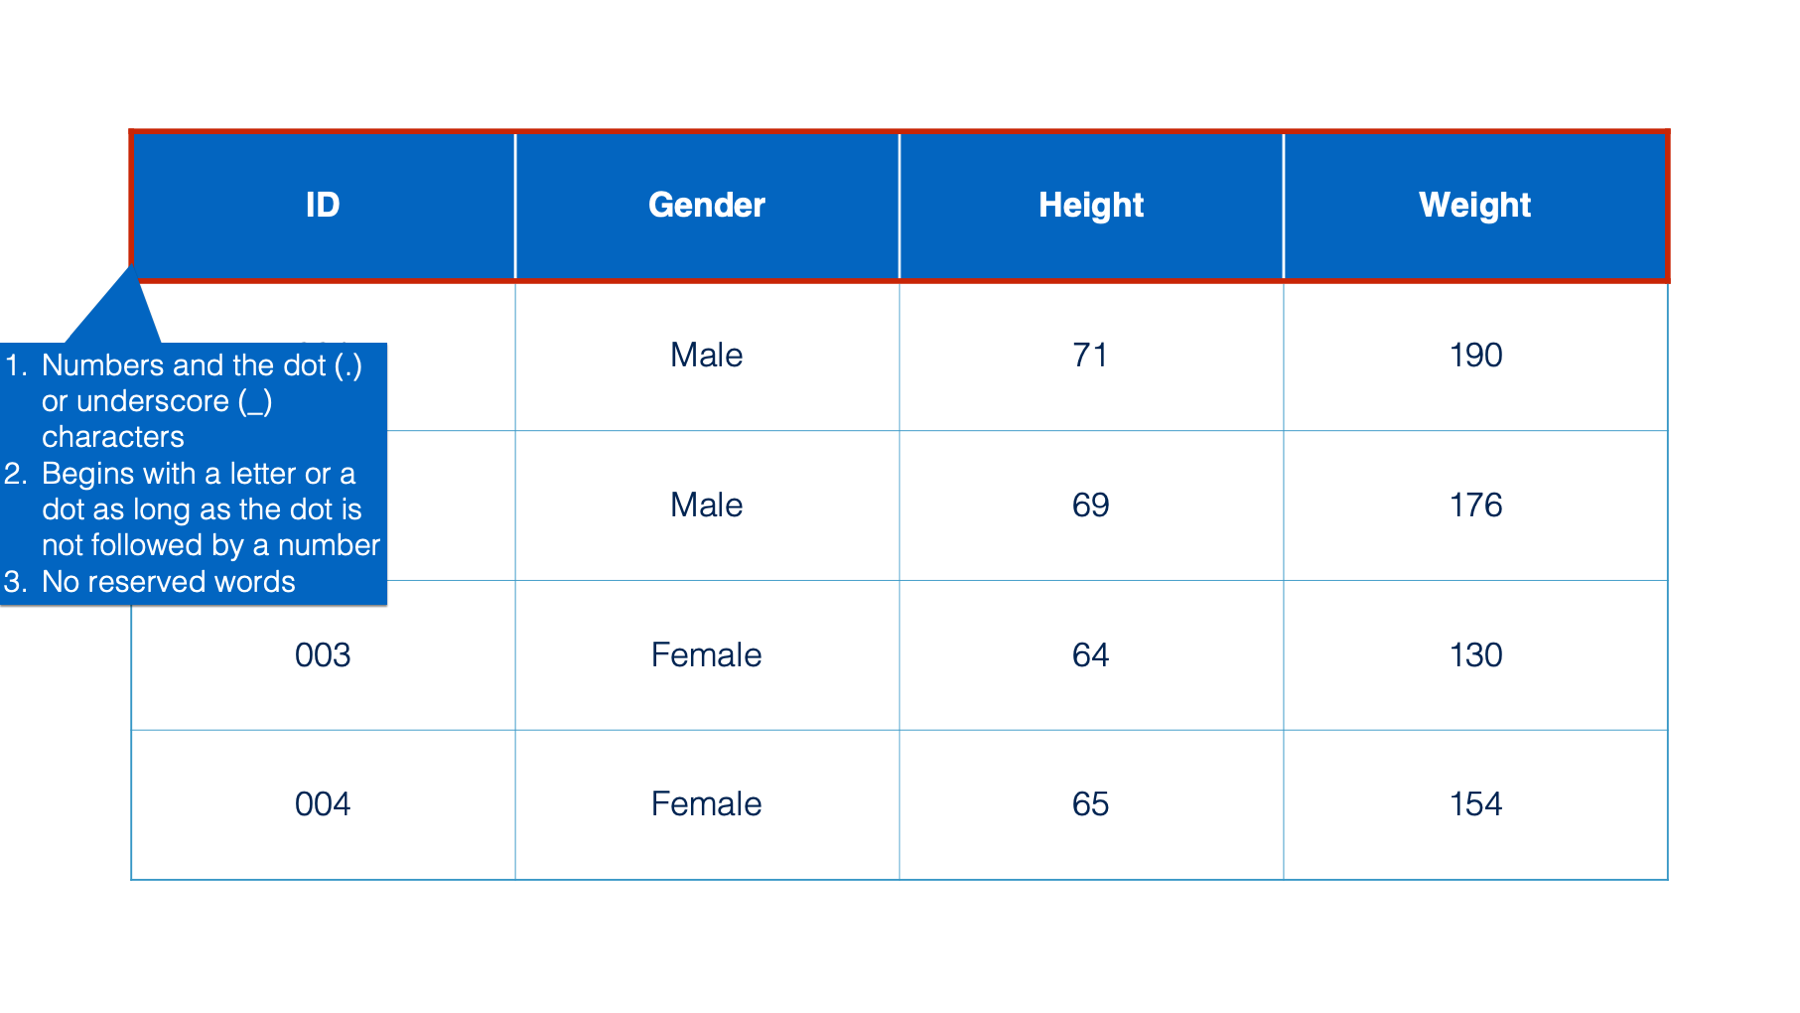
\includegraphics{chapters/what_is_r/table_column_name.png}

Moving from top to bottom across the table are \textbf{rows}, which are
sometimes referred to as records.

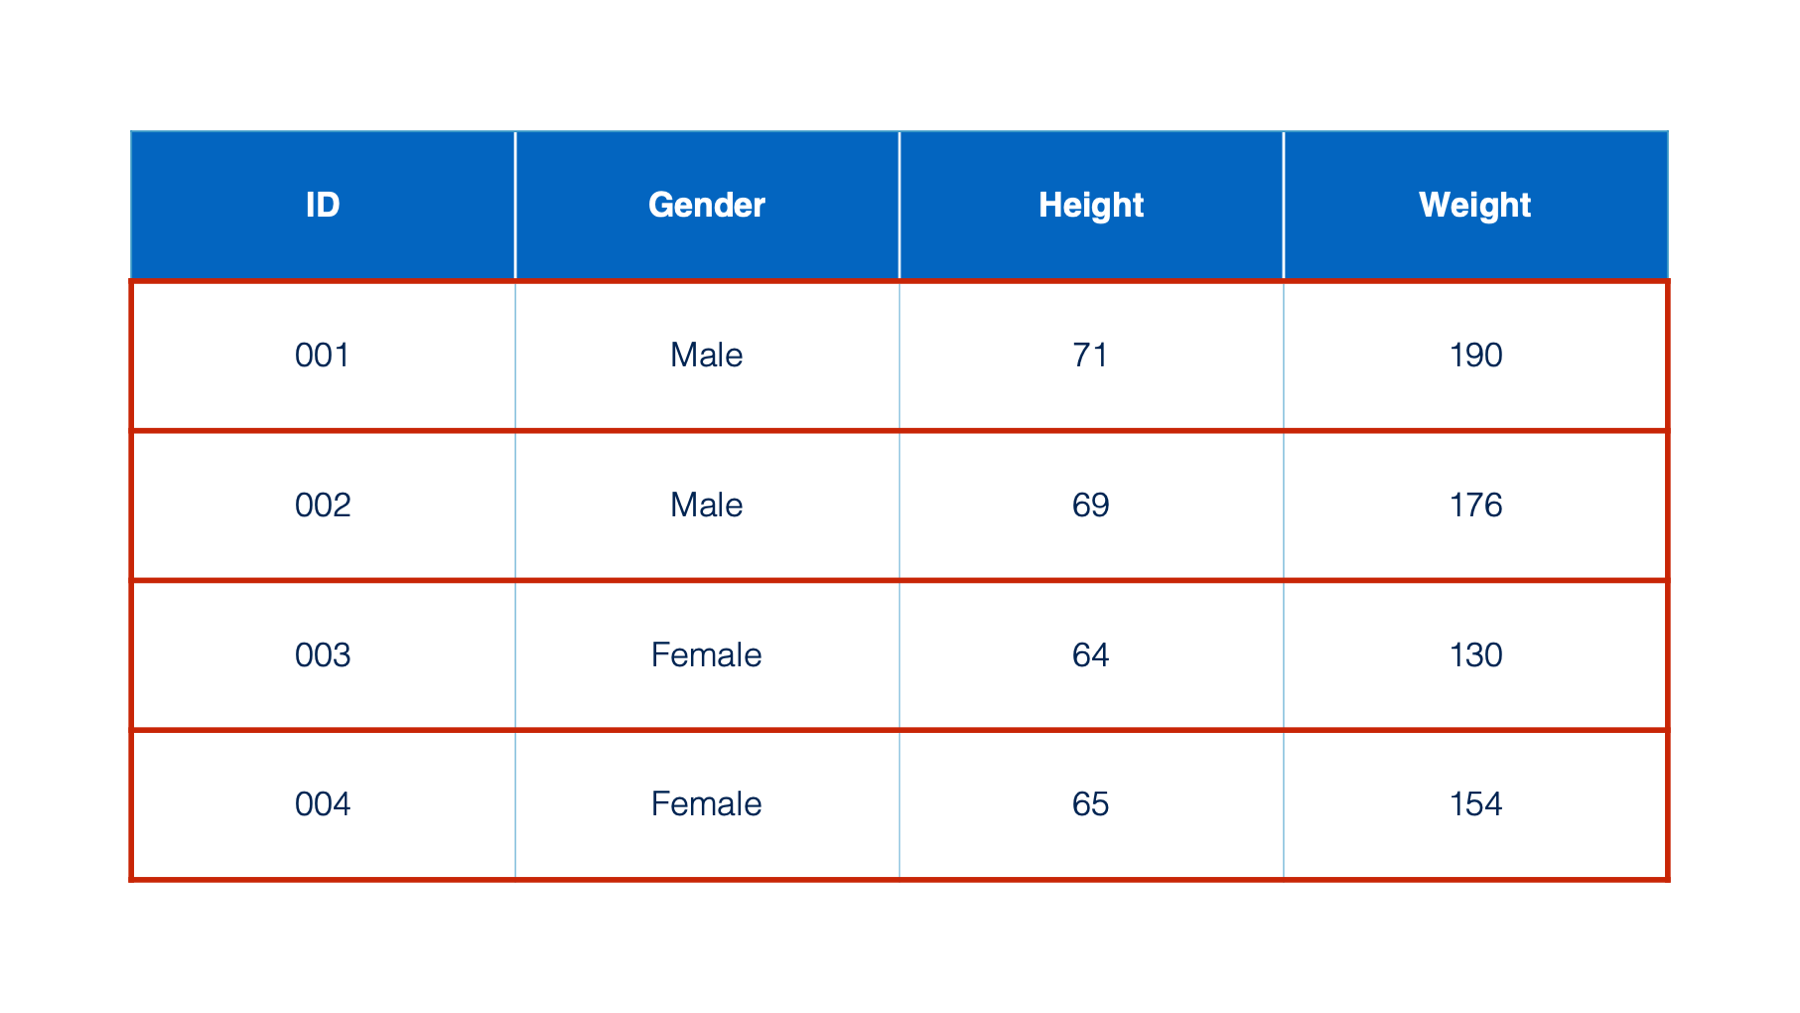
\includegraphics{chapters/what_is_r/table_rows.png}

Finally, the contents of each cell are called \textbf{values}.

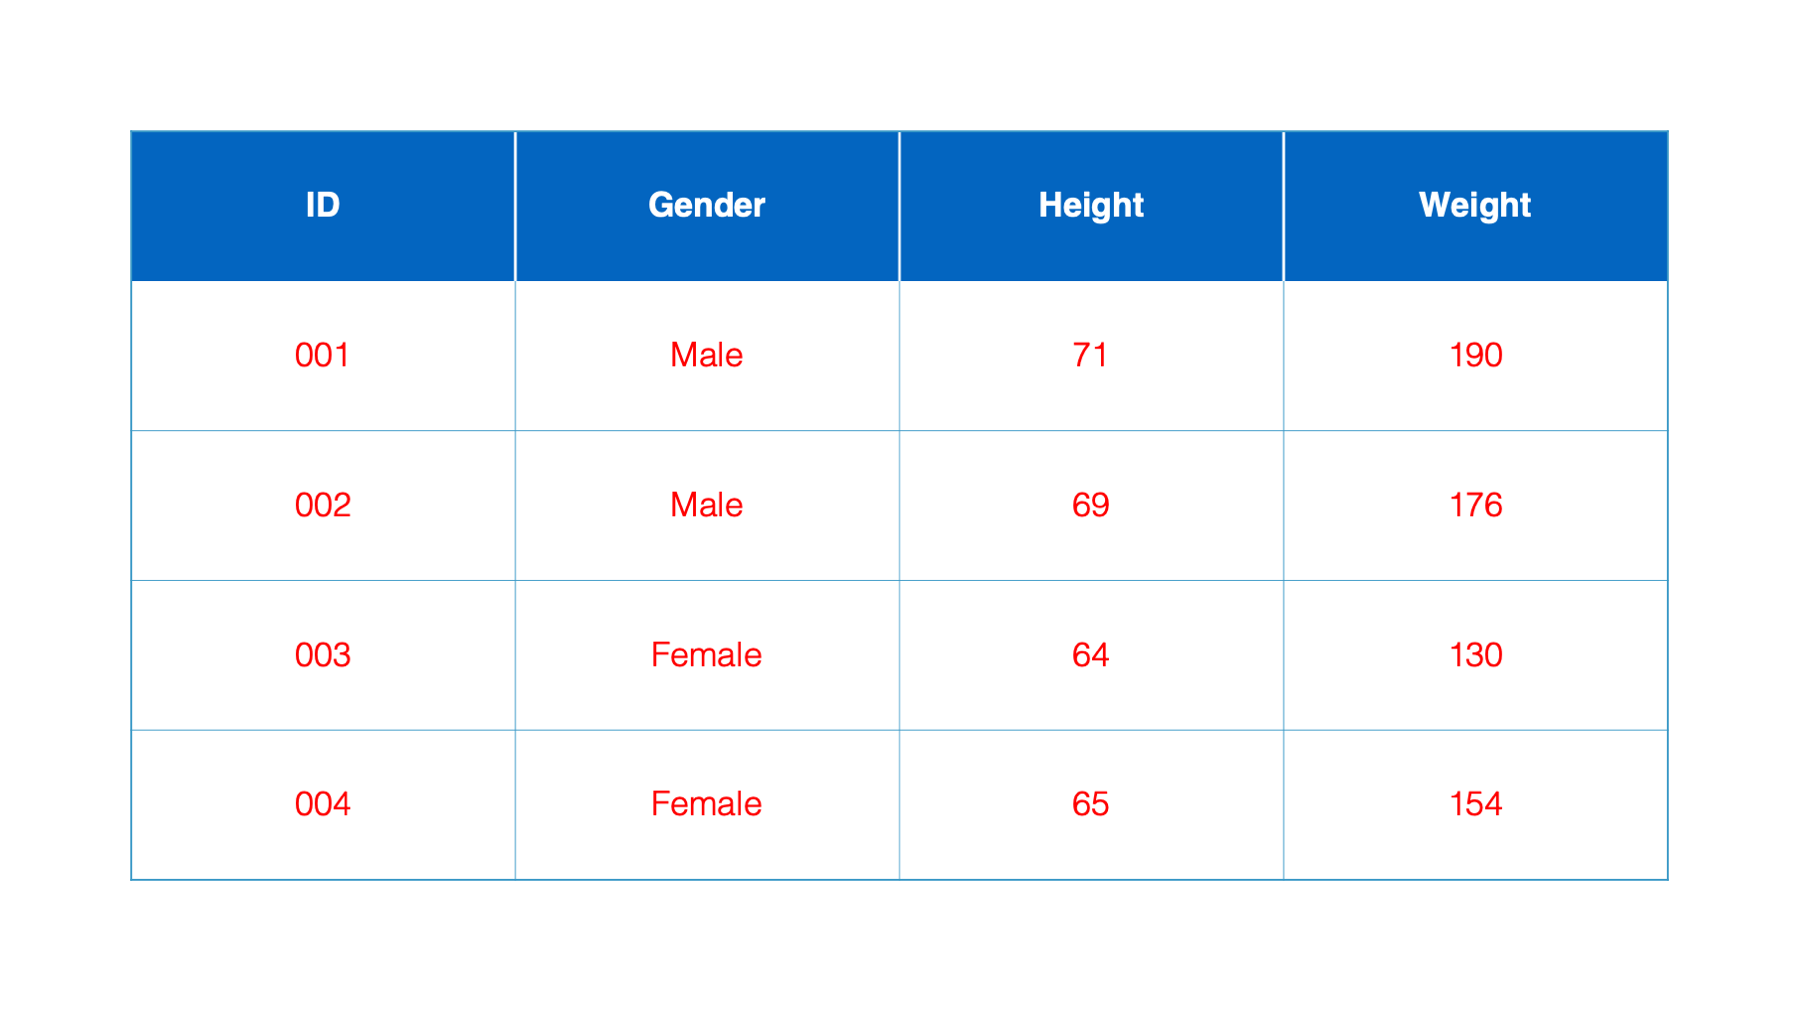
\includegraphics{chapters/what_is_r/table_values.png}

You should now be up to speed on some basic terminology used by R, as
well as other analytic, database, and spreadsheet programs. These terms
will be used repeatedly throughout the course.

\section{What is R?}\label{what-is-r-1}


\includegraphics{chapters/what_is_r/r_logo.png}

So, what is R? Well, R is an \textbf{open source} statistical
programming language that was created in the 1990's specifically for
data analysis. We will talk more about what open source means later, but
for now, just think of R as an easy (relatively 😂) way to ask your
computer to do math and statistics for you. More specifically, by the
end of this book you will be able to independently use R to transfer
data, manage data, analyze data, and present the results of your
analysis. Let's quickly take a closer look at each of these.

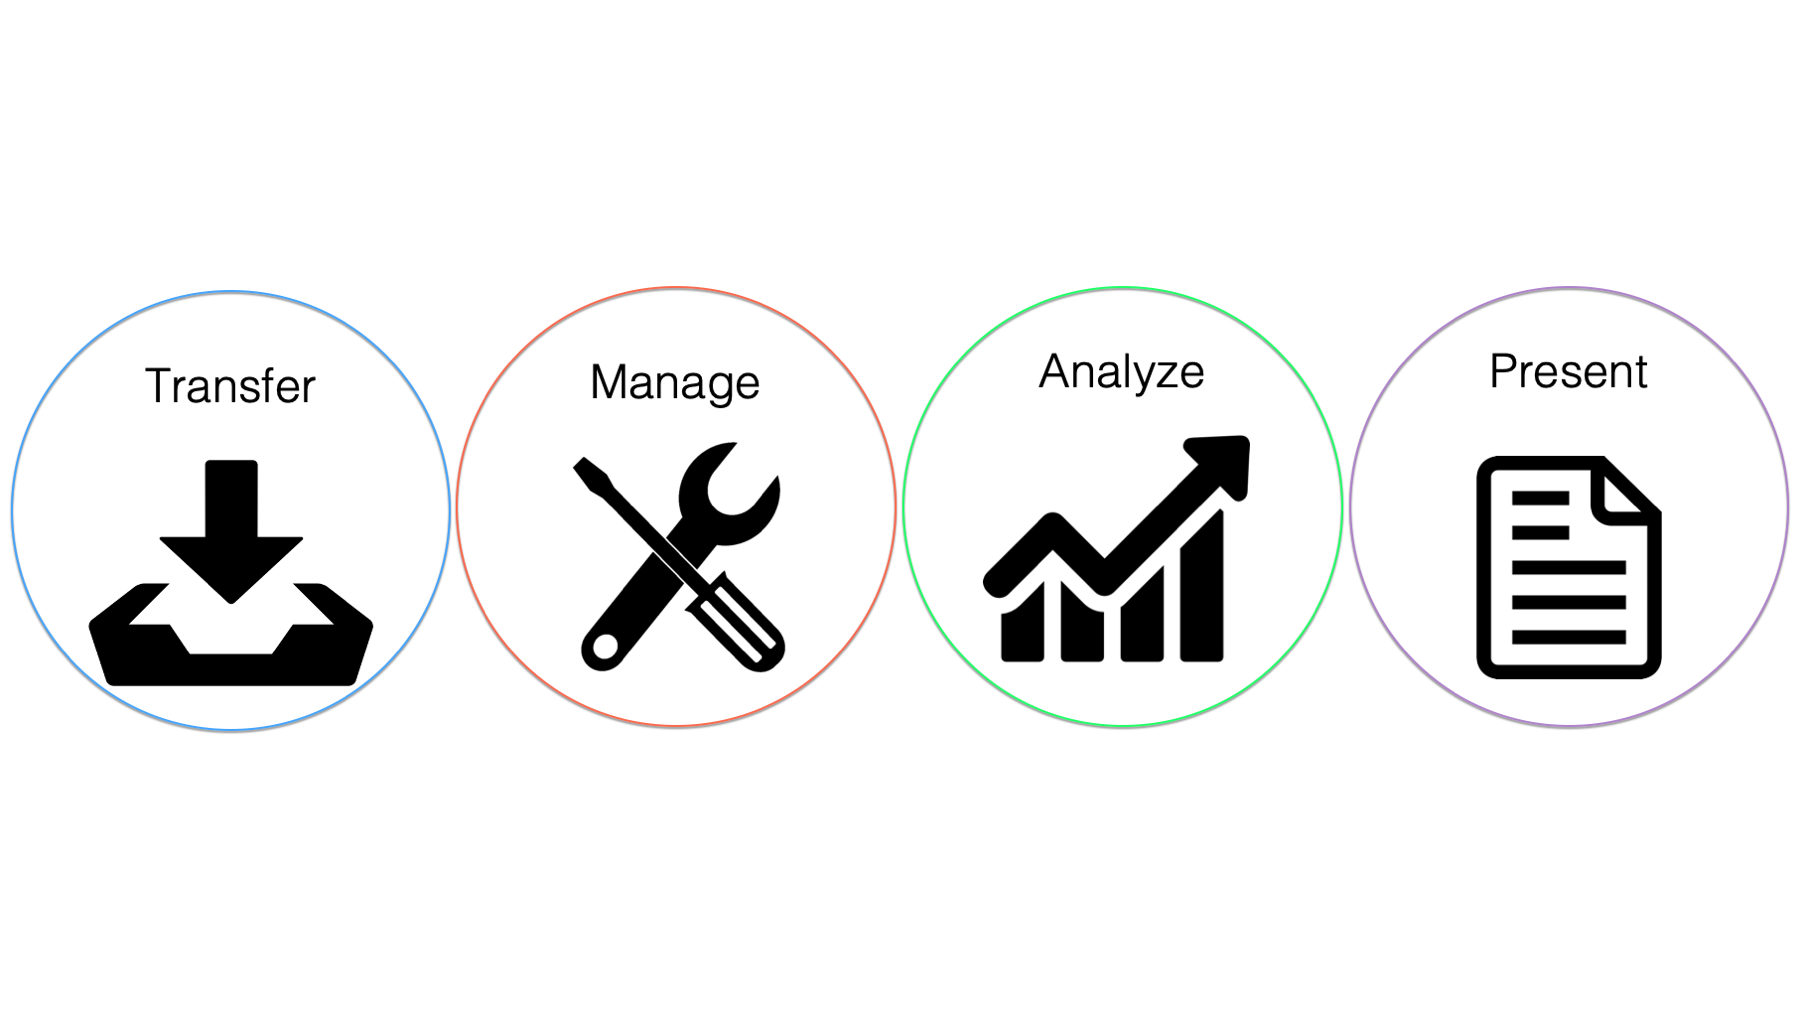
\includegraphics{chapters/what_is_r/competencies_overview.png}

\subsection{Transferring data}\label{transferring-data}

\includegraphics{chapters/what_is_r/competencies_transfer.png}

So, what do we mean by ``transfer data''? Well, individuals and
organizations store their data using different computer programs that
use different file types. Some common examples that you may come across
in epidemiology are database files, spreadsheets, raw data files, and
SAS data sets. No matter how the data is stored, you can't do anything
with it until you can get it into R, in a form that R can use, and in a
location that you can reach. In other words, transferring your data.
Therefore, among our first tasks in this course will be to transfer
data.

\subsection{Managing data}\label{managing-data}

\includegraphics{chapters/what_is_r/competencies_manage.png}

This isn't very specific, but managing data is all the things you may
have to do to your data to get it ready for analysis. You may also hear
people refer to this process as data wrangling or data munging. Some
specific examples of data management tasks include:

\begin{itemize}
\tightlist
\item
  \ul{Validating and cleaning data}. In other words, dealing with
  potential errors in the data.\\
\item
  \ul{Subsetting data}. For example, using only some of the columns or
  some of the rows.\\
\item
  \ul{Creating new variables}. For example, creating a BMI variable in a
  data frame that was sent to you with height and weight columns.\\
\item
  \ul{Combining data frames}. For example, combining sociodemographic
  data about study participants with data collected in the field during
  an intervention.
\end{itemize}

You may sometimes hear people refer to the 80/20 rule in reference to
data management. This ``rule'' says that in a typical data analysis
project, roughly 80\% of your time will be spent on data management and
only 20\% will be spent on the analysis itself. We can't provide you
with any empirical evidence (i.e., data) to back this claim up. But, as
people who have been involved in many projects that involve the
collection and analysis of data, we can tell you anecdotally that this
''rule'' is probably pretty close to being accurate in most cases.

Additionally, it's been our experience that most students of
epidemiology are required to take one or more classes that emphasize
methods for analyzing data; however, almost none of them have taken a
course that emphasizes data management!

Therefore, because data management is such a large component of most
projects that involve the collection and analysis of data, and because
most readers will have already been exposed to data analysis to a much
greater extent than data management, this course will heavily emphasize
the latter.

\subsection{Analyzing data}\label{analyzing-data}

\includegraphics{chapters/what_is_r/competencies_analysis.png}

As just discussed, this is probably the capability you most closely
associate with R, and there is no doubt that R is a powerful tool for
analyzing data. However, in this book we won't go beyond using R to
calculate basic descriptive statistics. For our purposes, descriptive
statistics include:

\begin{itemize}
\tightlist
\item
  \ul{Measures of central tendency}. For example, mean, median, and
  mode.\\
\item
  \ul{Measures of dispersion}. For example, variance and standard
  error.\\
\item
  \ul{Measures for describing categorical variables}. For example,
  counts and percentages.\\
\item
  \ul{Describing data using graphs and charts}. With R, we can describe
  our data using \href{https://www.r-graph-gallery.com/}{beautiful and
  informative graphs}.
\end{itemize}

\subsection{Presenting data}\label{presenting-data}

\includegraphics{chapters/what_is_r/competencies_present.png}

And finally, the ultimate goal is typically to present your findings in
some form or another. For example, a report, a website, or a journal
article. With R you can present your results in many different formats
with relative ease. In fact, this is one of our favorite things about R
and RStudio. In this class you will learn how to take your text,
tabular, or graphical results and then publish them in many different
formats including Microsoft Word, html files that can be viewed in web
browsers, and pdf documents. Let's take a look at some examples.

\begin{enumerate}
\def\labelenumi{\arabic{enumi}.}
\tightlist
\item
  \textbf{Microsoft Word documents}.
  \href{https://www.dropbox.com/s/6l1ikp6wbyue9bd/chap_2_example_word_docI.docx?dl=0}{Click
  here} to view an example report created for one of our research
  projects in Microsoft Word.\\
\item
  \textbf{PDF documents}.
  \href{https://www.dropbox.com/s/hheuyv5qcabf197/chap_2_example_pdf.pdf?dl=0}{Click
  here} to view a data dictionary we created in PDF format.\\
\item
  \textbf{HTML files}. Hypertext Markup Language (HTML) files are what
  you are looking at whenever you view a webpage. You can use R to
  create HTML files that others can view in their web browser. You can
  email them these files to view in their web browser, or you can make
  them available for others to view online just like any other website.
  \href{https://brad-cannell.github.io/detect_recruitment_dashboard/}{Click
  here} to view an example dashboard we created for one of our research
  projects.\\
\item
  \textbf{Web applications}. You can even use R to create full-fledged
  web applications. View the
  \href{https://shiny.rstudio.com/gallery/}{RStudio website} to see some
  examples.
\end{enumerate}

\chapter{Navigating the RStudio
Interface}\label{navigating-the-rstudio-interface}

If you followed along with the previous chapters, you have R and RStudio
installed on your computer and you have some idea of what R and RStudio
are. At this point, it can be common for people to open RStudio and get
totally overwhelmed. \emph{``What am I looking at?''} \emph{''What do I
click first?''} \emph{``Where do I even start?''} Don't worry if these,
or similar, thoughts have crossed your mind. You are in good company and
we will start to clear some of them up in this chapter.

When we load RStudio, we should see a screen that looks very similar to
Figure~\ref{fig-rstudio} below. There, we see three \textbf{panes}, and
each pane has multiple tabs.

\begin{figure}

\centering{

\includegraphics{chapters/navigating_rstudio/rstudio.png}

}

\caption{\label{fig-rstudio}The default RStudio user interface.}

\end{figure}%

\section{The console pane}\label{the-console-pane}

The first pane we are going to talk about is the
\textbf{console/terminal/background jobs} pane.

\begin{figure}

\centering{

\includegraphics{chapters/navigating_rstudio/console.png}

}

\caption{\label{fig-console}The R Console.}

\end{figure}%

It's called the ``console/terminal/background jobs'' pane because it has
three tabs we can click on by default: ``console'', ``terminal'', and
``background jobs''. However, we will refer to this pane as the
``console pane'' and will mostly ignore the terminal and background jobs
tabs for now. We aren't ignoring them because they aren't useful;
instead, we are ignoring them because using them isn't essential for
anything we will discuss in this chapter, and we want to keep things as
simple as possible for now.

The \hyperref[glossary-console]{console} is the most basic way to
interact with R. We can type a command to R into the console prompt (the
prompt looks like ``\textgreater{}'') and R will respond to what we
type. For example, below we typed ``1 + 1,'' pressed the return/enter
key, and the R console returned the sum of the numbers 1 and 1.

\begin{figure}

\centering{

\includegraphics{chapters/navigating_rstudio/one_plus_one.png}

}

\caption{\label{fig-one-plus-one}Doing some addition in the R console.}

\end{figure}%

The number 1 we see in brackets before the 2 (i.e., {[}1{]}) is telling
us that this line of results starts with the first result. That fact is
obvious here because there is only one result. So, let's look at a
result that spans multiple lines to make this idea clearer.

\begin{figure}

\centering{

\includegraphics{chapters/navigating_rstudio/seq_function.png}

}

\caption{\label{fig-seq-function}Demonstrating a function that returns
multiple results.}

\end{figure}%

In Figure~\ref{fig-seq-function} we see examples of a couple of new
concepts that are worth discussing.

First, as promised, we have more than one line of results (or output).
The first line of results starts with a 1 in brackets (i.e., {[}1{]}),
which indicates that this line of results starts with the first result.
In this case, the first result is the number 2. The second line of
results starts with a 29 in brackets (i.e., {[}29{]}), which indicates
that this line of results starts with the twenty-ninth result. In this
case, the twenty-ninth result is the number 58. If we count the numbers
in the first line, there should be 28 -- results 1 through 28. We also
want to make it clear that ``1'' and ``29'' are \emph{NOT} results
themselves. They are just helping us count the number of results per
line.

The second new thing that you may have noticed in
Figure~\ref{fig-seq-function} is our use of a \textbf{function}.
Functions are a \textbf{BIG DEAL} in R. So much so that R is called a
\emph{functional language}. We don't really need to know all the details
of what that means; however, we should know that, in general, everything
we \emph{do} in R we will \emph{do} with a function. By contrast,
everything we \emph{create} in R will be an \emph{object}. If we wanted
to make an analogy between the R language and the English language, we
could think of functions as verbs -- they \emph{do} things -- and
objects as nouns -- they \emph{are} things. This distinction likely
seems abstract and confusing at the moment, but we will make it more
concrete soon.

Most functions in R begin with the function name followed by
parentheses. For example, \texttt{seq()}, \texttt{sum()}, and
\texttt{mean()}.

\emph{Question}: What is the name of the function we used in the example
above?

\emph{Answer}: We used the \texttt{seq()} function -- short for sequence
- in the example above.

You may notice that there are three pairs of words, equal symbols, and
numbers that are separated by commas inside the \texttt{seq()} function.
They are, \texttt{from\ =\ 2}, \texttt{to\ =\ 100}, and
\texttt{by\ =\ 2}. The words \texttt{from}, \texttt{to}, and \texttt{by}
are all \hyperref[glossary-arguments]{arguments} to the \texttt{seq()}
function. We will learn more about functions and arguments later. For
now, just know that arguments \emph{give functions the information they
need to give us the result we want}.

In this case, the \texttt{seq()} function
\hyperref[glossary-returns]{returns} a sequence of numbers. But first,
we had to give it information about where that sequence should start,
where it should end, and how many steps should be in the middle. Above,
the sequence began with the value we \hyperref[glossary-pass]{passed} to
the \texttt{from} argument (i.e., 2), it ended with the value we passed
to the \texttt{to} argument (i.e., 100), and it increased at each step
by the number we passed to the \texttt{by} argument (i.e., 2). So, 2, 4,
6, 8 \ldots{} 100.

Whether you realize it or not, we've covered some important programming
terms while discussing the \texttt{seq()} function above. Before we move
on to discussing RStudio's other panes, let's quickly review and
reinforce a few of terms we will use repeatedly in this book.

\begin{itemize}
\item
  \hyperref[glossary-arguments]{Arguments}: Arguments always live
  \emph{inside} the parentheses of R functions and receive information
  the function needs to generate the result we want.
\item
  \hyperref[glossary-pass]{Pass}: In programming lingo, we \emph{pass} a
  value to a function argument. For example, in the function call
  \texttt{seq(from\ =\ 2,\ to\ =\ 100,\ by\ =\ 2)} we could say that we
  \emph{passed} a value of 2 to the \texttt{from} argument, we
  \emph{passed} a value of 100 to the \texttt{to} argument, and we
  \emph{passed} a value of 2 to the \texttt{by} argument.
\item
  \hyperref[glossary-return]{Return}: Instead of saying, ``the
  \texttt{seq()} function \emph{gives us} a sequence of
  numbers\ldots{}'' we say, ``the \texttt{seq()} function \emph{returns}
  a sequence of numbers\ldots{}'' In programming lingo, functions
  \emph{return} one or more results.
\end{itemize}

\begin{tcolorbox}[enhanced jigsaw, rightrule=.15mm, breakable, colback=white, bottomtitle=1mm, title=\textcolor{quarto-callout-note-color}{\faInfo}\hspace{0.5em}{Note}, colframe=quarto-callout-note-color-frame, opacityback=0, coltitle=black, colbacktitle=quarto-callout-note-color!10!white, opacitybacktitle=0.6, toptitle=1mm, bottomrule=.15mm, left=2mm, leftrule=.75mm, titlerule=0mm, toprule=.15mm, arc=.35mm]

🗒\textbf{Side Note:} The \texttt{seq()} function isn't particularly
important or noteworthy. We essentially chose it at random to illustrate
some key points. However, arguments, passing values, and return values
are extremely important concepts and we will return to them many times.

\end{tcolorbox}

\section{The environment pane}\label{the-environment-pane}

The second pane we are going to talk about is the
environment/history/connections pane in
Figure~\ref{fig-environment-pane}. However, we will mostly refer to it
as the environment pane and we will mostly ignore the history and
connections tab. We aren't ignoring them because they aren't useful;
rather, we are ignoring them because using them isn't essential for
anything we will discuss anytime soon, and we want to keep things as
simple as possible.

\begin{figure}

\centering{

\includegraphics{chapters/navigating_rstudio/environment_pane.png}

}

\caption{\label{fig-environment-pane}The environment pane}

\end{figure}%

The Environment pane shows you all the \textbf{objects} that R can
currently use for data management or analysis. In this picture,
Figure~\ref{fig-environment-pane} our environment is empty. Let's create
an object and add it to our environment.

\begin{figure}

\centering{

\includegraphics{chapters/navigating_rstudio/environment_pane2.png}

}

\caption{\label{fig-environment-pane2}The vector x in the global
environment.}

\end{figure}%

Here we see that we created a new object called \texttt{x}, which now
appears in our \textbf{Global Environment}.
Figure~\ref{fig-environment-pane2} This gives us another great
opportunity to discuss some new concepts.

First, we created the \texttt{x} object in the console by
\emph{assigning} the value 2 to the letter x. We did this by typing
``x'' followed by a less than symbol (\textless), a dash symbol (-), and
the number 2. R is kind of unique in this way. we have never seen
another programming language (although I'm sure they are out there) that
uses \texttt{\textless{}-} to assign values to variables. By the way,
\texttt{\textless{}-} is called the assignment operator (or assignment
arrow), and ''assign'' here means ``make x contain 2'' or ``put 2 inside
x.''

In many other languages you would write that as \texttt{x\ =\ 2}. But,
for whatever reason, in R it is \texttt{\textless{}-}. Unfortunately,
\texttt{\textless{}-} is more awkward to type than \texttt{=}.
Fortunately, RStudio gives us a keyboard shortcut to make it easier. To
type the assignment operator in RStudio, just hold down Option + - (dash
key) on a Mac or Alt + - (dash key) on a PC and RStudio will insert
\texttt{\textless{}-} complete with spaces on either side of the arrow.
This may still seem awkward at first, but you will get used to it.

\begin{tcolorbox}[enhanced jigsaw, rightrule=.15mm, breakable, colback=white, bottomtitle=1mm, title=\textcolor{quarto-callout-note-color}{\faInfo}\hspace{0.5em}{Note}, colframe=quarto-callout-note-color-frame, opacityback=0, coltitle=black, colbacktitle=quarto-callout-note-color!10!white, opacitybacktitle=0.6, toptitle=1mm, bottomrule=.15mm, left=2mm, leftrule=.75mm, titlerule=0mm, toprule=.15mm, arc=.35mm]

🗒\textbf{Side Note:} A note about using the letter ``x'': By convention,
the letter ``x'' is a widely used variable name. You will see it used a
lot in example documents and online. However, there is nothing special
about the letter x. We could have just as easily used any other letter
(\texttt{a\ \textless{}-\ 2}), word
(\texttt{variable\ \textless{}-\ 2}), or descriptive name
(\texttt{my\_favorite\_number\ \textless{}-\ 2}) that is allowed by R.

\end{tcolorbox}

Second, you can see that our Global Environment now includes the object
\texttt{x}, which has a value of 2. In this case, we would say that
\texttt{x} is a \textbf{numeric vector} of length 1 (i.e., it has one
value stored in it). We will talk more about vectors and vector types
soon. For now, just notice that objects that you can manipulate or
analyze in R will appear in your Global Environment.

\begin{tcolorbox}[enhanced jigsaw, rightrule=.15mm, breakable, colback=white, bottomtitle=1mm, title=\textcolor{quarto-callout-warning-color}{\faExclamationTriangle}\hspace{0.5em}{Warning}, colframe=quarto-callout-warning-color-frame, opacityback=0, coltitle=black, colbacktitle=quarto-callout-warning-color!10!white, opacitybacktitle=0.6, toptitle=1mm, bottomrule=.15mm, left=2mm, leftrule=.75mm, titlerule=0mm, toprule=.15mm, arc=.35mm]

⚠️\textbf{Warning:} R is a \textbf{case sensitive} language. That means
that uppercase x (X) and lowercase x (x) are different things to R. So,
if you assign 2 to lower case x (\texttt{x\ \textless{}-\ 2}). And then
later ask R to tell what number you stored in uppercase X, you will get
an error
(\texttt{Error:\ object\ \textquotesingle{}X\textquotesingle{}\ not\ found}).

\end{tcolorbox}

\section{The files pane}\label{the-files-pane}

Next, let's talk about the Files/Plots/Packages/Help/Viewer pane (that's
a mouthful). Figure~\ref{fig-files-pane}

\begin{figure}

\centering{

\includegraphics{chapters/navigating_rstudio/files_pane.png}

}

\caption{\label{fig-files-pane}The Files/Plots/Packages/Help/Viewer
pane.}

\end{figure}%

Again, some of these tabs are more applicable for us than others. For
us, the \textbf{files} tab and the \textbf{help} tab will probably be
the most useful. You can think of the files tab as a mini Finder window
(for Mac) or a mini File Explorer window (for PC). The help tab is also
extremely useful once you get acclimated to it.

\begin{figure}

\centering{

\includegraphics{chapters/navigating_rstudio/help.png}

}

\caption{\label{fig-help}The help tab.}

\end{figure}%

For example, in the screenshot above Figure~\ref{fig-help} we typed the
\texttt{seq} into the search bar. The help pane then shows us a page of
documentation for the \texttt{seq()} function. The documentation
includes a brief description of what the function does, outlines all the
arguments the \texttt{seq()} function recognizes, and, if you scroll
down, gives examples of using the \texttt{seq()} function. Admittedly,
this help documentation can seem a little like reading Greek (assuming
you don't speak Greek) at first. But, you will get more comfortable
using it with practice. We hated the help documentation when we were
learning R. Now, we use it \emph{all the time}.

\section{The source pane}\label{the-source-pane}

There is actually a fourth pane available in RStudio. If you click on
the icon shown below you will get the following dropdown box with a list
of files you can create. Figure~\ref{fig-source1}

\begin{figure}

\centering{

\includegraphics{chapters/navigating_rstudio/source1.png}

}

\caption{\label{fig-source1}Click the new source file icon.}

\end{figure}%

If you click any of these options, a new pane will appear. We will
arbitrarily pick the first option -- R Script.

\begin{figure}

\centering{

\includegraphics{chapters/navigating_rstudio/source2.png}

}

\caption{\label{fig-source2}New source file options.}

\end{figure}%

When we do, a new pane appears. It's called the \textbf{source pane}. In
this case, the source pane contains an untitled R Script. We won't get
into the details now because we don't want to overwhelm you, but soon
you will do the majority of your R programming in the source pane.

\begin{figure}

\centering{

\includegraphics{chapters/navigating_rstudio/source3.png}

}

\caption{\label{fig-source3}A blank R script in the source pane.}

\end{figure}%

\section{RStudio preferences}\label{rstudio-preferences}

Finally, We're going to recommend that you change a few settings in
RStudio before we move on. Start by clicking \texttt{Tools}, and then
\texttt{Global\ Options} in RStudio's menu bar, which probably runs
horizontally across the top of your computer's screen.

\begin{figure}

\centering{

\includegraphics{chapters/navigating_rstudio/preferences1.png}

}

\caption{\label{fig-preferences1}Select the preferences menu on Mac.}

\end{figure}%

In the \texttt{General} tab, we recommend turning off the
\texttt{Restore\ .Rdata\ into\ workspace\ at\ startup} option. We also
recommend setting the \texttt{Save\ workspace\ .Rdata\ on\ exit}
dropdown to \texttt{Never}. Finally, we recommend turning off the
\texttt{Always\ save\ history\ (even\ when\ not\ saving\ .Rdata)}
option.

\begin{figure}

\centering{

\includegraphics{chapters/navigating_rstudio/preferences3.png}

}

\caption{\label{fig-preferences3}General options tab.}

\end{figure}%

We change our editor theme to Twilight in the \texttt{Appearance} tab.
We aren't necessarily recommending that you change your theme -- this is
entirely personal preference -- we're just letting you know why our
screenshots will look different from here on out.

\begin{figure}

\centering{

\includegraphics{chapters/navigating_rstudio/preferences4.png}

}

\caption{\label{fig-preferences4}Appearance tab.}

\end{figure}%

It's likely that you still have lots of questions at this point. That's
totally natural. However, we hope you now feel like you have some idea
of what you are looking at when you open RStudio. Most of you will
naturally get more comfortable with RStudio as we move through the book.
For those of you who want more resources now, here are some suggestions.

\begin{enumerate}
\def\labelenumi{\arabic{enumi}.}
\item
  \href{https://rstudio.com/resources/cheatsheets/}{RStudio IDE
  cheatsheet}
\item
  \href{https://moderndive.com/1-getting-started.html\#r-rstudio}{ModernDive:
  What are R and RStudio?}
\end{enumerate}

\chapter{Speaking R's Language}\label{speaking-rs-language}

It has been our experience that students often come into statistical
programming courses thinking they will be heavy in math or statistics.
In reality, our R courses are probably much closer to a foreign language
course. There is no doubt that we need a foundational understanding of
math and statistics to understand the results we get from R, but R will
take care of most of the complicated stuff for us. We only need to learn
how to ask R to do what we want it to do. To some extent, this entire
book is about learning to communicate with R, but in this chapter we
will briefly introduce the R programming language from the 30,000-foot
level.

\section{\texorpdfstring{R is a
\emph{language}}{R is a language}}\label{r-is-a-language}

In the same way that many people use the English language to communicate
with each other, we will use the R programming language to communicate
with R. Just like the English language, the R language comes complete
with its own structure and vocabulary. Unfortunately, just like the
English language, it also includes some weird exceptions and occasional
miscommunications. We've already seen a couple examples of commands
written to R in the R programming language. Specifically:

\begin{Shaded}
\begin{Highlighting}[]
\CommentTok{\# Store the value 2 in the variable x}
\NormalTok{x }\OtherTok{\textless{}{-}} \DecValTok{2}
\CommentTok{\# Print the contents of x to the screen}
\NormalTok{x}
\end{Highlighting}
\end{Shaded}

\begin{verbatim}
[1] 2
\end{verbatim}

and

\begin{Shaded}
\begin{Highlighting}[]
\CommentTok{\# Print an example number sequence to the screen}
\FunctionTok{seq}\NormalTok{(}\AttributeTok{from =} \DecValTok{2}\NormalTok{, }\AttributeTok{to =} \DecValTok{100}\NormalTok{, }\AttributeTok{by =} \DecValTok{2}\NormalTok{)}
\end{Highlighting}
\end{Shaded}

\begin{verbatim}
 [1]   2   4   6   8  10  12  14  16  18  20  22  24  26  28  30  32  34  36  38
[20]  40  42  44  46  48  50  52  54  56  58  60  62  64  66  68  70  72  74  76
[39]  78  80  82  84  86  88  90  92  94  96  98 100
\end{verbatim}

\begin{tcolorbox}[enhanced jigsaw, rightrule=.15mm, breakable, colback=white, bottomtitle=1mm, title=\textcolor{quarto-callout-note-color}{\faInfo}\hspace{0.5em}{Note}, colframe=quarto-callout-note-color-frame, opacityback=0, coltitle=black, colbacktitle=quarto-callout-note-color!10!white, opacitybacktitle=0.6, toptitle=1mm, bottomrule=.15mm, left=2mm, leftrule=.75mm, titlerule=0mm, toprule=.15mm, arc=.35mm]

🗒\textbf{Side Note:} The gray boxes you see above are called R code
chunks and we created them (and this entire book) using something called
\href{https://quarto.org/}{Quarto files}. Can you believe that you can
write an entire book with R and RStudio? How cool is that? You will
learn to use Quarto files later in this book. Quarto is great because it
allows you to mix R code with narrative text and multimedia content as
we've done throughout the page you're currently looking at. This makes
it really easy for us to add context and aesthetic appeal to our
results.

\end{tcolorbox}

\section{The R interpreter}\label{the-r-interpreter}

Question: We keep talking about ``speaking'' to R, but when you speak to
R using the R language, who are you actually speaking to?

Well, you are speaking to something called the \textbf{R interpreter}.
The R interpreter takes the commands we've written in the R language,
sends them to our computer to do the actual work (e.g., get the mean of
a set of numbers), and then translates the results of that work back to
us in a form that we humans can understand (e.g., the mean is 25.5). At
this stage, one of the key concepts for you to understand about the R
language is that is \textbf{extremely literal!} Understanding the
literal nature of R is important because it will be the underlying cause
of a lot of errors in our R code.

\section{Errors}\label{errors}

No matter what we write next, you are going to get errors in your R
code. We still get errors in our R code every single time we write R
code. However, our hope is that this section will help you begin to
understand \emph{why} you are getting errors when you get them and
provide us with a common language for discussing errors.

So, what exactly do we mean when we say that the R interpreter is
extremely literal? Well, in the Navigating RStudio chapter, we already
told you that R is a \textbf{case sensitive} language. Again, that means
that uppercase x (X) and lowercase x (x) are different things to R. So,
if you assign 2 to lowercase x (\texttt{x\ \textless{}-\ 2}). And then
later ask R to tell what number you stored in upper case X; you will get
an error
(\texttt{Error:\ object\ \textquotesingle{}X\textquotesingle{}\ not\ found}).

\begin{Shaded}
\begin{Highlighting}[]
\NormalTok{x }\OtherTok{\textless{}{-}} \DecValTok{2}
\NormalTok{X}
\end{Highlighting}
\end{Shaded}

\begin{verbatim}
Error in eval(expr, envir, enclos): object 'X' not found
\end{verbatim}

Specifically, this is an example of a
\hyperref[glossary-logic-error]{logic error}. Meaning, R understands
what you are \emph{asking} it to do -- you want it to print the contents
of the uppercase X object to the screen. However, it can't complete your
request because you are asking it to do something that doesn't logically
make sense -- print the contents of a thing that doesn't exist.
Remember, R is literal and it will not try to guess that you actually
\emph{meant} to ask it to print the contents of lowercase x.

Another general type of error is known as a \textbf{syntax error}. In
programming languages, \hyperref[glossary-syntax]{syntax} refers to the
rules of the language. You can sort of think of this as the grammar of
the language. In English, we could say something like, ``giving dog
water drink.'' This sentence is grammatically completely incorrect;
however, most of you would roughly be able to figure out what we're
asking you to do based on your life experience and knowledge of the
situational context. The R interpreter, as awesome as it is, would not
be able to make an assumption about what we want it to do. In this case,
the R interpreter would say, ``I don't know what you're asking me to
do.'' When the R interpreter says, ``I don't know what you're asking me
to do,'' we've made a syntax error.

Throughout the rest of the book, we will try to point out situations
where R programmers often encounter errors and how you may be able to
address them. The remainder of this chapter will discuss some key
components of R's syntax and the data structures (i.e., ways of storing
data) that the R syntax interacts with.

\section{Functions}\label{functions}

R is a
\href{https://en.wikipedia.org/wiki/Functional_programming}{functional
programming language}, which simply means that
\hyperref[glossary-functions]{functions} play a central role in the R
language. But what are functions? Well, factories are a common analogy
used to represent functions. In this analogy, arguments are raw material
inputs that go into the factory. For example, steel and rubber. The
function is the factory where all the work takes place -- converting raw
materials into the desired output. Finally, the factory output
represents the returned results. In this case, bicycles.

\begin{figure}[H]

{\centering \includegraphics{chapters/speaking_r/factory1.png}

}

\caption{A factory making bicycles.}

\end{figure}%

To make this concept more concrete, in the
\href{../navigating_rstudio/navigating_rstudio.qmd}{Navigating RStudio}
chapter we used the \texttt{seq()} function as a factory. Specifically,
we wrote \texttt{seq(from\ =\ 2,\ to\ =\ 100,\ by\ =\ 2)}. The inputs
(arguments) were \texttt{from}, \texttt{to}, and \texttt{by}. The output
(returned result) was a set of numbers that went from 2 to 100 by 2's.
Most functions, like the \texttt{seq()} function, will be a word or word
part followed by parentheses. Other examples are the \texttt{sum()}
function for addition and the \texttt{mean()} function to calculate the
average value of a set of numbers.

\begin{figure}[H]

{\centering \includegraphics{chapters/speaking_r/factory2.png}

}

\caption{A function factory making numbers.}

\end{figure}%

\subsection{Passing values to function
arguments}\label{passing-values-to-function-arguments}

When we supply a value to a function argument, that is called
``passing'' a value to the argument. Let's take another look at the
sequence function we previously wrote and use it to help us with this
discussion.

\begin{Shaded}
\begin{Highlighting}[]
\CommentTok{\# Create a sequence of numbers beginning at 2 and ending at 100, incremented by 2.}
\FunctionTok{seq}\NormalTok{(}\AttributeTok{from =} \DecValTok{2}\NormalTok{, }\AttributeTok{to =} \DecValTok{100}\NormalTok{, }\AttributeTok{by =} \DecValTok{2}\NormalTok{)}
\end{Highlighting}
\end{Shaded}

\begin{verbatim}
 [1]   2   4   6   8  10  12  14  16  18  20  22  24  26  28  30  32  34  36  38
[20]  40  42  44  46  48  50  52  54  56  58  60  62  64  66  68  70  72  74  76
[39]  78  80  82  84  86  88  90  92  94  96  98 100
\end{verbatim}

In the code above, we \emph{passed} the value \texttt{2} to the
\texttt{from} argument, we \emph{passed} the value \texttt{100} to the
\texttt{to} argument, and we \emph{passed} the value \texttt{2} to the
\texttt{by} argument. How do we know we passed the value \texttt{2} to
the \texttt{from} argument? We know because we wrote
\texttt{from\ =\ 2}. To R, this means ``pass the value \texttt{2} to the
\texttt{from} argument,'' and it is an example of passing a value
\emph{by name}. Alternatively, we could have also gotten the same result
if we had passed the same values to the \texttt{seq()} function \emph{by
position}. What does that mean? We'll explain, but first take a look at
the following R code.

\begin{Shaded}
\begin{Highlighting}[]
\CommentTok{\# Create a sequence of numbers beginning at 2 and ending at 100, incremented by 2.}
\FunctionTok{seq}\NormalTok{(}\DecValTok{2}\NormalTok{, }\DecValTok{100}\NormalTok{, }\DecValTok{2}\NormalTok{)}
\end{Highlighting}
\end{Shaded}

\begin{verbatim}
 [1]   2   4   6   8  10  12  14  16  18  20  22  24  26  28  30  32  34  36  38
[20]  40  42  44  46  48  50  52  54  56  58  60  62  64  66  68  70  72  74  76
[39]  78  80  82  84  86  88  90  92  94  96  98 100
\end{verbatim}

How is code different from the code chunk before it? You got it! We
didn't explicitly write the names of the function arguments inside of
the \texttt{seq()} function. So, how did we get the same results? We got
the same results because R allows us to pass values to function
arguments by name \emph{or} by position. When we pass values to a
function \emph{by position}, R will pass the first input value to the
first function argument, the second input value to the second function
argument, the third input value to the third function argument, and so
on.

But how do we know what the first, second, and third arguments to a
function are? Do you remember our discussion about RStudio's
\hyperref[the-files-pane]{help tab} in the previous chapter? There, we
saw the documentation for the \texttt{seq()} function.

\begin{figure}[H]

{\centering \includegraphics{chapters/speaking_r/help.png}

}

\caption{The help tab.}

\end{figure}%

In the ``Usage'' section of the documentation for the \texttt{seq()}
function, we can see that all of the arguments that the \texttt{seq()}
function accepts. These documentation files are a little cryptic until
you get used to them but look directly underneath the part that says
``\#\# Default S3 method.'' There, it tells us that the \texttt{seq()}
function understands the \texttt{from}, \texttt{to}, \texttt{by},
\texttt{length.out}, \texttt{along.with}, and \texttt{...} arguments.
The \texttt{from} argument is first argument to the \texttt{seq()}
function because it is listed there first, the \texttt{to} argument is
second argument to the \texttt{seq()} function because it is listed
there second, and so on. It is really that simple. Therefore, when we
type \texttt{seq(2,\ 100,\ 2)}, R automatically translates it to
\texttt{seq(from\ =\ 2,\ to\ =\ 100,\ by\ =\ 2)}. And this is called
passing values to function arguments by position.

\begin{tcolorbox}[enhanced jigsaw, rightrule=.15mm, breakable, colback=white, bottomtitle=1mm, title=\textcolor{quarto-callout-note-color}{\faInfo}\hspace{0.5em}{Note}, colframe=quarto-callout-note-color-frame, opacityback=0, coltitle=black, colbacktitle=quarto-callout-note-color!10!white, opacitybacktitle=0.6, toptitle=1mm, bottomrule=.15mm, left=2mm, leftrule=.75mm, titlerule=0mm, toprule=.15mm, arc=.35mm]

🗒\textbf{Side Note:} As an aside, we can view the documentation for any
function by typing \texttt{?function\ name} into the R console and then
pressing the enter/return key. For example, we can type \texttt{?seq} to
view the documentation for the \texttt{seq()} function.

\end{tcolorbox}

Passing values to our functions by position has the benefit of making
our code more compact, we don't have to write out all the function
names. But, as you might have already guessed, passing values to our
functions by position also has some potential risks. First, it makes our
code harder to read. If we give our code to someone who has never used
the \texttt{seq()} function before, they will have to guess (or look up)
what purpose 2, 100, and 2 serve. When we pass the values to the
function by name, their purpose is typically easier to figure out even
if we've never used a particular function before. The second, and
potentially more important, risk is that we may accidentally pass a
value to a different argument than the one we intended. For example,
what if we mistakenly think the order of the arguments to the
\texttt{seq()} function is \texttt{from}. \texttt{by}, \texttt{to}? In
that case, we might write the following code:

\begin{Shaded}
\begin{Highlighting}[]
\CommentTok{\# Create a sequence of numbers beginning at 2 and ending at 100, incremented by 2.}
\FunctionTok{seq}\NormalTok{(}\DecValTok{2}\NormalTok{, }\DecValTok{2}\NormalTok{, }\DecValTok{100}\NormalTok{)}
\end{Highlighting}
\end{Shaded}

\begin{verbatim}
[1] 2
\end{verbatim}

Notice that R still gives us a result, but it isn't the result we want!
What happened? Well, we passed the values 2, 2, and 100 to the
\texttt{seq()} function \emph{by position}, which R translated to
\texttt{seq(from\ =\ 2,\ to\ =\ 2,\ by\ =\ 100)} because \texttt{from}
is the first argument in the \texttt{seq()} function, \texttt{to} is the
second argument in the \texttt{seq()} function, and \texttt{by} is the
third argument in the \texttt{seq()} function.

Quick review: is this an example of a syntax error or a logic error?

This is a logic error. We used perfectly valid R syntax in the code
above, but we mistakenly asked R to do something different than we
actually wanted it to do. In this simple example, it's easy to see that
this result is very different than what we were expecting and try to
figure out what we did wrong. But that won't always be the case.
Therefore, we need to be really careful when passing values to function
arguments by position.

One final note on passing values to functions. When we pass values to R
functions \emph{by name}, we can pass them in any order we want. For
example:

\begin{Shaded}
\begin{Highlighting}[]
\CommentTok{\# Create a sequence of numbers beginning at 2 and ending at 100, incremented by 2.}
\FunctionTok{seq}\NormalTok{(}\AttributeTok{from =} \DecValTok{2}\NormalTok{, }\AttributeTok{to =} \DecValTok{100}\NormalTok{, }\AttributeTok{by =} \DecValTok{2}\NormalTok{)}
\end{Highlighting}
\end{Shaded}

\begin{verbatim}
 [1]   2   4   6   8  10  12  14  16  18  20  22  24  26  28  30  32  34  36  38
[20]  40  42  44  46  48  50  52  54  56  58  60  62  64  66  68  70  72  74  76
[39]  78  80  82  84  86  88  90  92  94  96  98 100
\end{verbatim}

and

\begin{Shaded}
\begin{Highlighting}[]
\CommentTok{\# Create a sequence of numbers beginning at 2 and ending at 100, incremented by 2.}
\FunctionTok{seq}\NormalTok{(}\AttributeTok{to =} \DecValTok{100}\NormalTok{, }\AttributeTok{by =} \DecValTok{2}\NormalTok{, }\AttributeTok{from =} \DecValTok{2}\NormalTok{)}
\end{Highlighting}
\end{Shaded}

\begin{verbatim}
 [1]   2   4   6   8  10  12  14  16  18  20  22  24  26  28  30  32  34  36  38
[20]  40  42  44  46  48  50  52  54  56  58  60  62  64  66  68  70  72  74  76
[39]  78  80  82  84  86  88  90  92  94  96  98 100
\end{verbatim}

return the exact same values. Why? Because we explicitly told R which
argument to pass each value to \emph{by name}. Of course, just because
we \emph{can} do something doesn't mean we \emph{should} do it. We
really shouldn't rearrange argument order like this unless there is a
good reason.

\section{Objects}\label{objects}

In addition to functions, the R programming language also includes
objects. In the Navigating RStudio chapter we created an object called
\texttt{x} with a value of 2 using the \texttt{x\ \textless{}-\ 2} R
code. In general, you can think of objects as anything that lives in
your R global environment. Objects may be single variables (also called
vectors in R) or entire data sets (also called data frames in R).

Objects can be a confusing concept at first. We think it's because it is
hard to precisely define exactly what an object is. We'll say two things
about this. First, you're probably overthinking it (because we've
overthought it too). When we use R, we create and save stuff. We have to
call that stuff something in order to talk about it or write books about
it. Somebody decided we would call that stuff ``objects.'' The second
thing we'll say is that this becomes much less abstract when we finally
get to a place where you can really get your hands dirty doing some R
programming.

\begin{figure}[H]

{\centering \includegraphics{chapters/speaking_r/objects.png}

}

\caption{Creating the x object.}

\end{figure}%

Sometimes it can be useful to relate the R language to English grammar.
That is, when you are writing R code you can roughly think of functions
as verbs and objects as nouns. Just like nouns \emph{are} things in the
English language, and verbs \emph{do} things in the English language,
objects \emph{are} things and functions \emph{do} things in the R
language.

So, in the \texttt{x\ \textless{}-\ 2} command \texttt{x} is the object
and \texttt{\textless{}-} is the function. ``Wait! Didn't you just tell
us that functions will be a word followed by parentheses?'' Fair
question. Technically, we said, ``\emph{Most} functions will be a word,
or word part, followed by parentheses.'' Just like English, R has
exceptions. All \textbf{operators} in R are also functions. Operators
are symbols like \texttt{+}, \texttt{-}, \texttt{=}, and
\texttt{\textless{}-}. There are many more operators, but you will
notice that they all \emph{do} things. In this case, they add, subtract,
and assign values to objects.

\includegraphics{chapters/speaking_r/language.png}

\section{Comments}\label{comments}

And finally, there are comments. If our R code is a conversation we are
having with the R interpreter, then comments are your inner thoughts
taking place during the conversation. Comments don't actually mean
anything to R, but they will be extremely important for you. You
actually already saw a couple examples of comments above.

\begin{Shaded}
\begin{Highlighting}[]
\CommentTok{\# Store the value 2 in the variable x}
\NormalTok{x }\OtherTok{\textless{}{-}} \DecValTok{2}
\CommentTok{\# Print the contents of x to the screen}
\NormalTok{x}
\end{Highlighting}
\end{Shaded}

\begin{verbatim}
[1] 2
\end{verbatim}

In this code chunk, ``\# Store the value 2 in the variable x'' and ``\#
Print the contents of x to the screen'' are both examples of comments.
Notice that they both start with the pound or hash sign (\#). The R
interpreter will ignore anything on the \emph{current line} that comes
after the hash sign. A carriage return (new line) ends the comment.
However, comments don't have to be written on their own line. They can
also be written on the same line as R code as long as put them after the
R code, like this:

\begin{Shaded}
\begin{Highlighting}[]
\NormalTok{x }\OtherTok{\textless{}{-}} \DecValTok{2} \CommentTok{\# Store the value 2 in the variable x}
\NormalTok{x      }\CommentTok{\# Print the contents of x to the screen}
\end{Highlighting}
\end{Shaded}

\begin{verbatim}
[1] 2
\end{verbatim}

Most beginning R programmers underestimate the importance of comments.
In the silly little examples above, the comments are not that useful.
However, comments will become extremely important as you begin writing
more complex programs. When working on projects, you will often need to
share your programs with others. Reading R code without any context is
really challenging -- even for experienced R programmers. Additionally,
even if your collaborators can surmise \emph{what} your R code is doing,
they may have no idea \emph{why} you are doing it. Therefore, your
comments should tell others what your code does (if it isn't completely
obvious), and more importantly, what your code is trying to accomplish.
Even if you aren't sharing your code with others, you may need to come
back and revise or reuse your code months or years down the line. You
may be shocked at how foreign the code \emph{you wrote} will seem months
or years after you wrote it. Therefore, comments are not just important
for others, they are also important for future you!

\begin{tcolorbox}[enhanced jigsaw, rightrule=.15mm, breakable, colback=white, bottomtitle=1mm, title=\textcolor{quarto-callout-note-color}{\faInfo}\hspace{0.5em}{Note}, colframe=quarto-callout-note-color-frame, opacityback=0, coltitle=black, colbacktitle=quarto-callout-note-color!10!white, opacitybacktitle=0.6, toptitle=1mm, bottomrule=.15mm, left=2mm, leftrule=.75mm, titlerule=0mm, toprule=.15mm, arc=.35mm]

🗒\textbf{Side Note:} RStudio has a handy little keyboard shortcut for
creating comments. On a Mac, type shift + command + C. On Windows, Shift
+ Ctrl + C.

\end{tcolorbox}

\begin{tcolorbox}[enhanced jigsaw, rightrule=.15mm, breakable, colback=white, bottomtitle=1mm, title=\textcolor{quarto-callout-note-color}{\faInfo}\hspace{0.5em}{Note}, colframe=quarto-callout-note-color-frame, opacityback=0, coltitle=black, colbacktitle=quarto-callout-note-color!10!white, opacitybacktitle=0.6, toptitle=1mm, bottomrule=.15mm, left=2mm, leftrule=.75mm, titlerule=0mm, toprule=.15mm, arc=.35mm]

🗒\textbf{Side Note:} Please put a space in between the pound/hash sign
and the rest of your text when writing comments. For example,
\texttt{\#\ here\ is\ my\ comment} instead of
\texttt{\#here\ is\ my\ comment}. It just makes the comment easier to
read.

\end{tcolorbox}

\section{Packages}\label{packages}

In addition to being a functional programming language, R is also a type
of programming language called an
\href{https://en.wikipedia.org/wiki/Open-source_software}{open source}
programming language. For our purposes, this has two big advantages.
First, it means that R is \textbf{FREE!} Second, it means that smart
people all around the world get to develop new \textbf{packages} for the
R language that can do cutting edge and/or very niche things.

That second advantage is probably really confusing if this is not a
concept you are already familiar with. For example, when you install
Microsoft Word on your computer all the code that makes that program
work is owned and Maintained by the Microsoft corporation. If you need
Word to do something that it doesn't currently do, your only option is
to make a feature request on Microsoft's website. Microsoft may or may
not every get around to fulfilling that request.

R works a little differently. When you downloaded R from the CRAN
website, you actually downloaded something called \textbf{Base R}. Base
R is maintained by the R Core Team. However, anybody -- \emph{even you}
-- can write your own code (called packages) that add new functions to
the R syntax. Like all functions, these new functions allow you to
\emph{do} things that you can't do (or can't do as easily) with Base R.

An analogy that we really like here is used by Ismay and Kim in
\href{https://moderndive.com/1-getting-started.html\#packages}{ModernDive}.

\begin{quote}
A good analogy for R packages is they are like apps you can download
onto a mobile phone. So R is like a new mobile phone: while it has a
certain amount of features when you use it for the first time, it
doesn't have everything. R packages are like the apps you can download
onto your phone from Apple's App Store or Android's Google
Play.\textsuperscript{1}
\end{quote}

So, when you get a new smart phone it comes with apps for making phone
calls, checking email, and sending text messages. But, what if you want
to listen to music on Spotify? You may or may not be able to do that
through your phone's web browser, but it's way more convenient and
powerful to download and install the Spotify app.

In this course, we will make extensive use of packages developed by
people and teams outside of the R Core Team. In particular, we will use
a number of related packages that are collectively known as the
\href{https://www.tidyverse.org/}{Tidyverse}. One of the most popular
packages in the tidyverse collection (and one of the most popular R
packages overall) is called the \texttt{dplyr} package for data
management.

In the same way that you have to download and install Spotify on your
mobile phone before you can use it, you have to download and install new
R packages on your computer before you can use the functions they
contain. Fortunately, R makes this really easy. For most packages, all
you have to do is run the \texttt{install.packages()} function in the R
console. For example, here is how you would install the \texttt{dplyr}
package.

\begin{Shaded}
\begin{Highlighting}[]
\CommentTok{\# Make sure you remember to wrap the name of the package in single or double quotes.}
\FunctionTok{install.packages}\NormalTok{(}\StringTok{"dplyr"}\NormalTok{)}
\end{Highlighting}
\end{Shaded}

Over time, you will download and install a lot of different packages.
All those packages with all of those new functions start to create a lot
of overhead. Therefore, R doesn't keep them loaded and available for use
at all times. Instead, \emph{every time} you open RStudio, you will have
to explicitly tell R which packages you want to use. So, when you close
RStudio and open it again, the only functions that you will be able to
use are Base R functions. If you want to use functions from any other
package (e.g., \texttt{dplyr}) you will have to tell R that you want to
do so using the \texttt{library()} function.

\begin{Shaded}
\begin{Highlighting}[]
\CommentTok{\# No quotes needed here}
\FunctionTok{library}\NormalTok{(dplyr)}
\end{Highlighting}
\end{Shaded}

Technically, loading the package with the \texttt{library()} function is
not the only way to use a function from a package you've downloaded. For
example, the \texttt{dplyr} package contains a function called
\texttt{filter()} that helps us keep or drop certain rows in a data
frame. To use this function, we have to first download the
\texttt{dplyr} package. Then we can use the filter function in one of
two different ways.

\begin{Shaded}
\begin{Highlighting}[]
\FunctionTok{library}\NormalTok{(dplyr)}
\FunctionTok{filter}\NormalTok{(states\_data, state }\SpecialCharTok{==} \StringTok{"Texas"}\NormalTok{) }\CommentTok{\# Keeps only the rows from Texas}
\end{Highlighting}
\end{Shaded}

The first way you already saw above. Load all the functions contained in
the \texttt{dplyr} package using the \texttt{library()} function. Then
use that function just like any other Base R function.

The second way is something called the \textbf{double colon syntax}. To
use the double colon syntax, you type the package name, two colons, and
the name of the function you want to use from the package. Here is an
example of the double colon syntax.

\begin{Shaded}
\begin{Highlighting}[]
\NormalTok{dplyr}\SpecialCharTok{::}\FunctionTok{filter}\NormalTok{(states\_data, state }\SpecialCharTok{==} \StringTok{"Texas"}\NormalTok{) }\CommentTok{\# Keeps only the rows from Texas}
\end{Highlighting}
\end{Shaded}

Most of the time you will load packages using the \texttt{library()}
function. However, we wanted to show you the double colon syntax because
you may come across it when you are reading R documentation and because
there are times when it makes sense to use this syntax.

\section{Programming style}\label{programming-style}

Finally, we want to discuss programming style. R can read any code you
write as long as you write it using valid R syntax. However, R code can
be much easier or harder for people (including you) to read depending on
how it's written. The \hyperref[coding-best-practices]{coding best
practices chapter} of this book gives complete details on writing R code
that is as easy as possible for \emph{people} to read. So, please make
sure to read it. It will make things so much easier for all of us!

\chapter{Let's Get Programming}\label{lets-get-programming}

In this chapter, we are going to tie together many of the concepts we've
learned so far, and you are going to create your first basic R program.
Specifically, you are going to write a program that simulates some data
and analyzes it.

\section{Simulating data}\label{simulating-data}

Data simulation can be really complicated, but it doesn't have to be. It
is simply the process of \emph{creating} data as opposed to
\emph{finding data in the wild}. This can be really useful in several
different ways.

\begin{enumerate}
\def\labelenumi{\arabic{enumi}.}
\item
  Simulating data is really useful for getting help with a problem you
  are trying to solve. Often, it isn't feasible for you to send other
  people the actual data set you are working on when you encounter a
  problem you need help with. Sometimes, it may not even be legally
  allowed (i.e., for privacy reasons). Instead of sending them your
  entire data set, you can simulate a little data set that recreates the
  challenge you are trying to address without all the other complexity
  of the full data set. As a bonus,we have often found that we end up
  figuring out the solution to the problem we're trying to solve as we
  recreate the problem in a simulated data set that we intended to share
  with others.
\item
  Simulated data can also be useful for learning about and testing
  statistical assumptions. In epidemiology, we use statistics to draw
  conclusions about populations of people we are interested in based on
  samples of people drawn from the population. Because we don't actually
  have data from \emph{all} the people in the population, we have to
  make some assumptions about the population based on what we find in
  our sample. When we simulate data, we know the truth about our
  population because we \emph{created} our population to have that
  truth. We can then use this simulated population to play ``what if''
  games with our analysis. \emph{What if we only sampled half as many
  people?} \emph{What if their heights aren't actually normally
  distributed?} \emph{What if we used a probit model instead of a logit
  model?} Going through this process and answering these questions can
  help us understand how much, and under what circumstances, we can
  trust the answers we found in the real world.
\end{enumerate}

So, let's go ahead and write a complete R program to simulate and
analyze some data. As we said, it doesn't have to be complicated. In
fact, in just a few lines of R code below we simulate and analyze some
data about a hypothetical class.

\begin{Shaded}
\begin{Highlighting}[]
\NormalTok{class }\OtherTok{\textless{}{-}} \FunctionTok{data.frame}\NormalTok{(}
  \AttributeTok{names   =} \FunctionTok{c}\NormalTok{(}\StringTok{"John"}\NormalTok{, }\StringTok{"Sally"}\NormalTok{, }\StringTok{"Brad"}\NormalTok{, }\StringTok{"Anne"}\NormalTok{),}
  \AttributeTok{heights =} \FunctionTok{c}\NormalTok{(}\DecValTok{68}\NormalTok{, }\DecValTok{63}\NormalTok{, }\DecValTok{71}\NormalTok{, }\DecValTok{72}\NormalTok{)}
\NormalTok{)}
\end{Highlighting}
\end{Shaded}

\begin{Shaded}
\begin{Highlighting}[]
\NormalTok{class}
\end{Highlighting}
\end{Shaded}

\begin{verbatim}
  names heights
1  John      68
2 Sally      63
3  Brad      71
4  Anne      72
\end{verbatim}

\begin{Shaded}
\begin{Highlighting}[]
\FunctionTok{mean}\NormalTok{(class}\SpecialCharTok{$}\NormalTok{heights)}
\end{Highlighting}
\end{Shaded}

\begin{verbatim}
[1] 68.5
\end{verbatim}

As you can see, this data frame contains the students' names and
heights. We also use the \texttt{mean()} function to calculate the
average height of the class. By the end of this chapter, you will
understand all the elements of this R code and how to simulate your own
data.

\section{Vectors}\label{vectors}

Vectors are the most fundamental data structure in R. Here, data
structure means ``container for our data.'' There are other data
structures as well; however, they are all built from vectors. That's why
we say vectors are the most fundamental data structure. Some of these
other structures include matrices, lists, and data frames. In this book,
we won't use matrices or lists much at all, so you can forget about them
for now. Instead, we will almost exclusively use data frames to hold and
manipulate our data. However, because data frames are built from
vectors, it can be useful to start by learning a little bit about them.
Let's create our first vector now.

\begin{Shaded}
\begin{Highlighting}[]
\CommentTok{\# Create an example vector}
\NormalTok{names }\OtherTok{\textless{}{-}} \FunctionTok{c}\NormalTok{(}\StringTok{"John"}\NormalTok{, }\StringTok{"Sally"}\NormalTok{, }\StringTok{"Brad"}\NormalTok{, }\StringTok{"Anne"}\NormalTok{)}
\CommentTok{\# Print contents to the screen}
\NormalTok{names}
\end{Highlighting}
\end{Shaded}

\begin{verbatim}
[1] "John"  "Sally" "Brad"  "Anne" 
\end{verbatim}

👆\textbf{Here's what we did above:}

\begin{itemize}
\item
  We \emph{created} a vector of names with the \texttt{c()} (short for
  combine) function.

  \begin{itemize}
  \item
    The vector contains four values: ``John'', ``Sally'', ``Brad'', and
    ``Anne''.
  \item
    All of the values are character strings (i.e., words). We know this
    because all of the values are wrapped with quotation marks.
  \item
    Here we used double quotes above, but we could have also used single
    quotes. We cannot, however, mix double and single quotes for each
    character string. For example,
    \texttt{c("John\textquotesingle{},\ ...)} won't work.
  \end{itemize}
\item
  We \emph{assigned} that vector of character strings to the word
  \texttt{names} using the \texttt{\textless{}-} function.

  \begin{itemize}
  \item
    R now recognizes \texttt{names} as an \textbf{object} that we can do
    things with.
  \item
    R programmers may refer to the names object as ``the names object'',
    ``the names vector'', or ``the names variable''. For our purposes,
    these all mean the same thing.
  \end{itemize}
\item
  We \emph{printed} the contents of the \texttt{names} object to the
  screen by typing the word ``names''.

  \begin{itemize}
  \tightlist
  \item
    R \textbf{returns} (shows us) the four character values (``John''
    ``Sally'' ``Brad'' ``Anne'') on the computer screen.
  \end{itemize}
\end{itemize}

Try copying and pasting the code above into the RStudio console on your
computer. You should notice the names vector appear in your
\textbf{global environment}. You may also notice that the global
environment pane gives you some additional information about this vector
to the right of its name. Specifically, you should see
\texttt{chr\ {[}1:4{]}\ "John"\ \ "Sally"\ "Brad"\ \ "Anne"}. This is R
telling us that \texttt{names} is a character vector (\texttt{chr}),
with four values (\texttt{{[}1:4{]}}), and the first four values are
\texttt{"John"\ \ "Sally"\ "Brad"\ \ "Anne"}.

\subsection{Vector types}\label{vector-types}

There are several different vector \textbf{types}, but each vector can
have only one type. The type of the vector above was character. We can
validate that with the \texttt{typeof()} function like so:

\begin{Shaded}
\begin{Highlighting}[]
\FunctionTok{typeof}\NormalTok{(names)}
\end{Highlighting}
\end{Shaded}

\begin{verbatim}
[1] "character"
\end{verbatim}

The other vector types that we will use in this book are double,
integer, and logical. Double vectors hold
\href{https://en.wikipedia.org/wiki/Real_number}{real numbers} and
integer vectors hold
\href{https://en.wikipedia.org/wiki/Integer}{integers}. Collectively,
double vectors and integer vectors are known as numeric vectors. Logical
vectors can only hold the values TRUE and FALSE. Here are some examples
of each:

\subsection{Double vectors}\label{double-vectors}

\begin{Shaded}
\begin{Highlighting}[]
\CommentTok{\# A numeric vector}
\NormalTok{my\_numbers }\OtherTok{\textless{}{-}} \FunctionTok{c}\NormalTok{(}\FloatTok{12.5}\NormalTok{, }\FloatTok{13.98765}\NormalTok{, pi)}
\NormalTok{my\_numbers}
\end{Highlighting}
\end{Shaded}

\begin{verbatim}
[1] 12.500000 13.987650  3.141593
\end{verbatim}

\begin{Shaded}
\begin{Highlighting}[]
\FunctionTok{typeof}\NormalTok{(my\_numbers)}
\end{Highlighting}
\end{Shaded}

\begin{verbatim}
[1] "double"
\end{verbatim}

\subsection{Integer vectors}\label{integer-vectors}

Creating integer vectors involves a weird little quirk of the R
language. For some reason, and we have no idea why, we must type an
``L'' behind the number to make it an integer.

\begin{Shaded}
\begin{Highlighting}[]
\CommentTok{\# An integer vector {-} first attempt}
\NormalTok{my\_ints\_1 }\OtherTok{\textless{}{-}} \FunctionTok{c}\NormalTok{(}\DecValTok{1}\NormalTok{, }\DecValTok{2}\NormalTok{, }\DecValTok{3}\NormalTok{)}
\NormalTok{my\_ints\_1}
\end{Highlighting}
\end{Shaded}

\begin{verbatim}
[1] 1 2 3
\end{verbatim}

\begin{Shaded}
\begin{Highlighting}[]
\FunctionTok{typeof}\NormalTok{(my\_ints\_1)}
\end{Highlighting}
\end{Shaded}

\begin{verbatim}
[1] "double"
\end{verbatim}

\begin{Shaded}
\begin{Highlighting}[]
\CommentTok{\# An integer vector {-} second attempt}
\CommentTok{\# Must put "L" behind the number to make it an integer. No idea why they chose "L".}
\NormalTok{my\_ints\_2 }\OtherTok{\textless{}{-}} \FunctionTok{c}\NormalTok{(}\DecValTok{1}\NormalTok{L, }\DecValTok{2}\NormalTok{L, }\DecValTok{3}\NormalTok{L)}
\NormalTok{my\_ints\_2}
\end{Highlighting}
\end{Shaded}

\begin{verbatim}
[1] 1 2 3
\end{verbatim}

\begin{Shaded}
\begin{Highlighting}[]
\FunctionTok{typeof}\NormalTok{(my\_ints\_2)}
\end{Highlighting}
\end{Shaded}

\begin{verbatim}
[1] "integer"
\end{verbatim}

\subsection{Logical vectors}\label{logical-vectors}

\begin{Shaded}
\begin{Highlighting}[]
\CommentTok{\# A logical vector}
\CommentTok{\# Type TRUE and FALSE in all caps}
\NormalTok{my\_logical }\OtherTok{\textless{}{-}} \FunctionTok{c}\NormalTok{(}\ConstantTok{TRUE}\NormalTok{, }\ConstantTok{FALSE}\NormalTok{, }\ConstantTok{TRUE}\NormalTok{)}
\NormalTok{my\_logical}
\end{Highlighting}
\end{Shaded}

\begin{verbatim}
[1]  TRUE FALSE  TRUE
\end{verbatim}

\begin{Shaded}
\begin{Highlighting}[]
\FunctionTok{typeof}\NormalTok{(my\_logical)}
\end{Highlighting}
\end{Shaded}

\begin{verbatim}
[1] "logical"
\end{verbatim}

Rather than have an abstract discussion about the particulars of each of
these vector types right now, we think it's best to wait and learn more
about them when they naturally arise in the context of a real challenge
we are trying to solve with data. At this point, just having some vague
idea that they exist is good enough.

\subsection{Factor vectors}\label{factor-vectors}

Above, we said that we would only work with three vector types in this
book: double, integer, and logical. Technically, that is true. Factors
aren't technically a vector type (we will explain below) but calling
them a vector type is close enough to true for our purposes. We will
briefly introduce you to factors here, and then discuss them in more
depth later in the chapter on {[}Numerical Descriptions of Categorical
Variables{]}. We cover them in greater depth there because factors are
most useful in the context of working with categorical data -- data that
is grouped into discrete categories. Some examples of categorical
variables commonly seen in public health data are sex, race or
ethnicity, and level of educational attainment.

In R, we can represent a categorical variable in multiple different
ways. For example, let's say that we are interested in recording
people's highest level of formal education completed in our data. The
discrete categories we are interested in are:

\begin{itemize}
\item
  1 = Less than high school
\item
  2 = High school graduate
\item
  3 = Some college
\item
  4 = College graduate
\end{itemize}

We could then create a numeric vector to record the level of educational
attainment for four hypothetical people as shown below.

\begin{Shaded}
\begin{Highlighting}[]
\CommentTok{\# A numeric vector of education categories}
\NormalTok{education\_num }\OtherTok{\textless{}{-}} \FunctionTok{c}\NormalTok{(}\DecValTok{3}\NormalTok{, }\DecValTok{1}\NormalTok{, }\DecValTok{4}\NormalTok{, }\DecValTok{1}\NormalTok{)}
\NormalTok{education\_num}
\end{Highlighting}
\end{Shaded}

\begin{verbatim}
[1] 3 1 4 1
\end{verbatim}

But what is less-than-ideal about storing our categorical data this way?
Well, it isn't obvious what the numbers in \texttt{education\_num} mean.
For the purposes of this example, we defined them above, but if we
didn't have that information then we would likely have no idea what
categories the numbers represent.

We could also create a character vector to record the level of
educational attainment for four hypothetical people as shown below.

\begin{Shaded}
\begin{Highlighting}[]
\CommentTok{\# A character vector of education categories}
\NormalTok{education\_chr }\OtherTok{\textless{}{-}} \FunctionTok{c}\NormalTok{(}
  \StringTok{"Some college"}\NormalTok{, }\StringTok{"Less than high school"}\NormalTok{, }\StringTok{"College graduate"}\NormalTok{, }
  \StringTok{"Less than high school"}
\NormalTok{)}
\NormalTok{education\_chr}
\end{Highlighting}
\end{Shaded}

\begin{verbatim}
[1] "Some college"          "Less than high school" "College graduate"     
[4] "Less than high school"
\end{verbatim}

But this strategy also has a few limitations that we will discuss in in
the chapter on {[}Numerical Descriptions of Categorical Variables{]}.
For now, we just need to quickly learn how to create and identify factor
vectors.

Typically, we don't \emph{create} factors from scratch. Instead, we
typically convert (or ``coerce'') an existing numeric or character
vector into a factor. For example, we can coerce \texttt{education\_num}
to a factor like this:

\begin{Shaded}
\begin{Highlighting}[]
\CommentTok{\# Coerce education\_num to a factor}
\NormalTok{education\_num\_f }\OtherTok{\textless{}{-}} \FunctionTok{factor}\NormalTok{(}
  \AttributeTok{x      =}\NormalTok{ education\_num,}
  \AttributeTok{levels =} \DecValTok{1}\SpecialCharTok{:}\DecValTok{4}\NormalTok{,}
  \AttributeTok{labels =} \FunctionTok{c}\NormalTok{(}
    \StringTok{"Less than high school"}\NormalTok{, }\StringTok{"High school graduate"}\NormalTok{, }\StringTok{"Some college"}\NormalTok{, }
    \StringTok{"College graduate"}
\NormalTok{  )}
\NormalTok{)}
\NormalTok{education\_num\_f}
\end{Highlighting}
\end{Shaded}

\begin{verbatim}
[1] Some college          Less than high school College graduate     
[4] Less than high school
4 Levels: Less than high school High school graduate ... College graduate
\end{verbatim}

👆 \textbf{Here's what we did above:}

\begin{itemize}
\item
  We used the \texttt{factor()} function to create a new factor version
  of \texttt{education\_num}.

  \begin{itemize}
  \item
    You can type \texttt{?factor} into your R console to view the help
    documentation for this function and follow along with the
    explanation below.
  \item
    The first argument to the \texttt{factor()} function is the
    \texttt{x} argument. The value passed to the \texttt{x} argument
    should be a vector of data. We passed the \texttt{education\_num}
    vector to the \texttt{x} argument.
  \item
    The second argument to the \texttt{factor()} function is the
    \texttt{levels} argument. This argument tells R the unique values
    that the new factor variable can take. We used the shorthand
    \texttt{1:4} to tell R that \texttt{education\_num\_f} can take the
    unique values 1, 2, 3, or 4.
  \item
    The third argument to the \texttt{factor()} function is the
    \texttt{labels} argument. The value passed to the \texttt{labels}
    argument should be a character vector of labels (i.e., descriptive
    text) for each value in the \texttt{levels} argument. The order of
    the labels in the character vector we pass to the \texttt{labels}
    argument should match the order of the values passed to the
    \texttt{levels} argument. For example, the ordering of
    \texttt{levels} and \texttt{labels} above tells R that \texttt{1}
    should be labeled with ``Less than high school'', \texttt{2} should
    be labeled with ``High school graduate'', etc.
  \end{itemize}
\item
  We used the assignment operator (\texttt{\textless{}-}) to save our
  new factor vector in our global environment as
  \texttt{education\_num\_f}.

  \begin{itemize}
  \item
    If we had used the name \texttt{education\_num} instead, then the
    previous values in the \texttt{education\_num} vector would have
    been replaced with the new values. That is sometimes what we want to
    happen. However, when it comes to creating factors, we typically
    keep the numeric version of the vector and create an additional
    factor version of the vector. We just often find that it can be
    useful to have both versions of the variable hanging around during
    the analysis process.
  \item
    We also use the \texttt{\_f} naming convention in our code. That
    means that when we create a new factor vector, we name it the same
    thing the original vector was named with the addition of
    \texttt{\_f} (for factor) at the end.
  \end{itemize}
\item
  We printed the vector to the screen. The values in
  \texttt{education\_num\_f} \emph{look} similar to the character
  strings displayed in \texttt{education\_chr}. Notice, however, that
  the values no longer have quotes around them and R displays
  \texttt{Levels:\ Less\ than\ high\ school\ High\ school\ graduate\ Some\ college\ College\ graduate}
  below the data values. This is R telling us the \emph{possible}
  categorical values that this factor could take on. This is a telltale
  sign that the vector being printed to the screen is a factor.
\end{itemize}

Interestingly, although R uses labels to make factors \emph{look} like
character vectors, they are still integer vectors under the hood. For
example:

\begin{Shaded}
\begin{Highlighting}[]
\FunctionTok{typeof}\NormalTok{(education\_num\_f)}
\end{Highlighting}
\end{Shaded}

\begin{verbatim}
[1] "integer"
\end{verbatim}

And we can still view them as such.

\begin{Shaded}
\begin{Highlighting}[]
\FunctionTok{as.numeric}\NormalTok{(education\_num\_f)}
\end{Highlighting}
\end{Shaded}

\begin{verbatim}
[1] 3 1 4 1
\end{verbatim}

It is also possible to coerce character vectors to factors. For example,
we can coerce \texttt{education\_chr} to a factor like so:

\begin{Shaded}
\begin{Highlighting}[]
\CommentTok{\# Coerce education\_chr to a factor}
\NormalTok{education\_chr\_f }\OtherTok{\textless{}{-}} \FunctionTok{factor}\NormalTok{(}
  \AttributeTok{x      =}\NormalTok{ education\_chr,}
  \AttributeTok{levels =} \FunctionTok{c}\NormalTok{(}
    \StringTok{"Less than high school"}\NormalTok{, }\StringTok{"High school graduate"}\NormalTok{, }\StringTok{"Some college"}\NormalTok{, }
    \StringTok{"College graduate"}
\NormalTok{  )}
\NormalTok{)}
\NormalTok{education\_chr\_f}
\end{Highlighting}
\end{Shaded}

\begin{verbatim}
[1] Some college          Less than high school College graduate     
[4] Less than high school
4 Levels: Less than high school High school graduate ... College graduate
\end{verbatim}

👆 \textbf{Here's what we did above:}

\begin{itemize}
\item
  We coerced a character vector (\texttt{education\_chr}) to a factor
  using the \texttt{factor()} function.
\item
  Because the levels \emph{are} character strings, there was no need to
  pass any values to the \texttt{labels} argument this time. Keep in
  mind, though, that the order of the values passed to the
  \texttt{levels} argument matters. It will be the order that the factor
  levels will be displayed in our analyses.
\end{itemize}

You might reasonably wonder why we would want to convert character
vectors to factors, but we will save that discussion for the chapter on
{[}Numerical Descriptions of Categorical Variables{]}.

\section{Data frames}\label{data-frames}

Vectors are useful for storing a single characteristic where all the
data is of the same type. However, in epidemiology, we typically want to
store information about many different characteristics of whatever we
happen to be studying. For example, we didn't just want the names of the
people in our class, we also wanted the heights. Of course, we can also
store the heights in a vector like so:

\begin{Shaded}
\begin{Highlighting}[]
\NormalTok{heights }\OtherTok{\textless{}{-}} \FunctionTok{c}\NormalTok{(}\DecValTok{68}\NormalTok{, }\DecValTok{63}\NormalTok{, }\DecValTok{71}\NormalTok{, }\DecValTok{72}\NormalTok{)}
\NormalTok{heights}
\end{Highlighting}
\end{Shaded}

\begin{verbatim}
[1] 68 63 71 72
\end{verbatim}

But this vector, in and of itself, doesn't tell us which height goes
with which person. When we want to create relationships between our
vectors, we can use them to build a data frame. For example:

\begin{Shaded}
\begin{Highlighting}[]
\CommentTok{\# Create a vector of names}
\NormalTok{names }\OtherTok{\textless{}{-}} \FunctionTok{c}\NormalTok{(}\StringTok{"John"}\NormalTok{, }\StringTok{"Sally"}\NormalTok{, }\StringTok{"Brad"}\NormalTok{, }\StringTok{"Anne"}\NormalTok{)}
\CommentTok{\# Create a vector of heights}
\NormalTok{heights }\OtherTok{\textless{}{-}} \FunctionTok{c}\NormalTok{(}\DecValTok{68}\NormalTok{, }\DecValTok{63}\NormalTok{, }\DecValTok{71}\NormalTok{, }\DecValTok{72}\NormalTok{)}
\CommentTok{\# Combine them into a data frame}
\NormalTok{class }\OtherTok{\textless{}{-}} \FunctionTok{data.frame}\NormalTok{(names, heights)}
\CommentTok{\# Print the data frame to the screen}
\NormalTok{class}
\end{Highlighting}
\end{Shaded}

\begin{verbatim}
  names heights
1  John      68
2 Sally      63
3  Brad      71
4  Anne      72
\end{verbatim}

👆\textbf{Here's what we did above:}

\begin{itemize}
\item
  We \emph{created} a data frame with the \texttt{data.frame()}
  function.

  \begin{itemize}
  \item
    The first argument we passed to the \texttt{data.frame()} function
    was a vector of names that we previously created.
  \item
    The second argument we passed to the \texttt{data.frame()} function
    was a vector of heights that we previously created.
  \end{itemize}
\item
  We \emph{assigned} that data frame to the word \texttt{class} using
  the \texttt{\textless{}-} function.

  \begin{itemize}
  \item
    R now recognizes \texttt{class} as an \textbf{object} that we can do
    things with.
  \item
    R programmers may refer to this class object as ``the class object''
    or ``the class data frame''. For our purposes, these all mean the
    same thing. We could also call it a data set, but that term isn't
    used much in R circles.
  \end{itemize}
\item
  We \emph{printed} the contents of the \texttt{class} object to the
  screen by typing the word ``class''.

  \begin{itemize}
  \tightlist
  \item
    R \textbf{returns} (shows us) the data frame on the computer screen.
  \end{itemize}
\end{itemize}

Try copying and pasting the code above into the RStudio console on your
computer. You should notice the \texttt{class} data frame appear in your
\textbf{global environment}. You may also notice that the global
environment pane gives you some additional information about this data
frame to the right of its name. Specifically, you should see
\texttt{4\ obs.\ of\ 2\ variables}. This is R telling us that
\texttt{class} has four rows or observations (\texttt{4\ obs.}) and two
columns or variables (\texttt{2\ variables}). If you click the little
blue arrow to the left of the data frame's name, you will see
information about the individual vectors that make up the data frame.

As a shortcut, instead of creating individual vectors and then combining
them into a data frame as we've done above, most R programmers will
create the vectors (columns) directly inside of the data frame function
like this:

\begin{Shaded}
\begin{Highlighting}[]
\CommentTok{\# Create the class data frame}
\NormalTok{class }\OtherTok{\textless{}{-}} \FunctionTok{data.frame}\NormalTok{(}
  \AttributeTok{names   =} \FunctionTok{c}\NormalTok{(}\StringTok{"John"}\NormalTok{, }\StringTok{"Sally"}\NormalTok{, }\StringTok{"Brad"}\NormalTok{, }\StringTok{"Anne"}\NormalTok{),}
  \AttributeTok{heights =} \FunctionTok{c}\NormalTok{(}\DecValTok{68}\NormalTok{, }\DecValTok{63}\NormalTok{, }\DecValTok{71}\NormalTok{, }\DecValTok{72}\NormalTok{)}
\NormalTok{) }\CommentTok{\# Closing parenthesis down here.}

\CommentTok{\# Print the data frame to the screen}
\NormalTok{class}
\end{Highlighting}
\end{Shaded}

\begin{verbatim}
  names heights
1  John      68
2 Sally      63
3  Brad      71
4  Anne      72
\end{verbatim}

As you can see, both methods produce the exact same result. The second
method, however, requires a little less typing and results in fewer
objects cluttering up your global environment. What we mean by that is
that the \texttt{names} and \texttt{heights} vectors won't exist
independently in your global environment. Rather, they will only exist
as columns of the \texttt{class} data frame.

You may have also noticed that when we created the \texttt{names} and
\texttt{heights} vectors (columns) directly inside of the
\texttt{data.frame()} function we used the equal sign (\texttt{=}) to
assign values instead of the assignment arrow (\texttt{\textless{}-}).
This is just one of those quirky R exceptions we talked about in the
chapter on speaking R's language. In fact, \texttt{=} and
\texttt{\textless{}-} can be used interchangeably in R. It is only by
convention that we usually use \texttt{\textless{}-} for assigning
values, but use \texttt{=} for assigning values to columns in data
frames. we don't know why this is the convention. If it were up to me,
we wouldn't do this. We would just pick \texttt{=} or
\texttt{\textless{}-} and use it in all cases where we want to assign
values. But, it isn't up to me and we gave up on trying to fight it a
long time ago. Your R programming life will be easier if you just learn
to assign values this way -- even if it's dumb. 🤷

\begin{tcolorbox}[enhanced jigsaw, rightrule=.15mm, breakable, colback=white, bottomtitle=1mm, title=\textcolor{quarto-callout-warning-color}{\faExclamationTriangle}\hspace{0.5em}{Warning}, colframe=quarto-callout-warning-color-frame, opacityback=0, coltitle=black, colbacktitle=quarto-callout-warning-color!10!white, opacitybacktitle=0.6, toptitle=1mm, bottomrule=.15mm, left=2mm, leftrule=.75mm, titlerule=0mm, toprule=.15mm, arc=.35mm]

⚠️\textbf{Warning:} By definition, all columns in a data frame must have
the same length (i.e., number of rows). That means that each vector you
create when building your data frame must have the same number of values
in it. For example, the class data frame above has four names and four
heights. If we had only entered three heights, we would have gotten the
following error:
\texttt{Error\ in\ data.frame(names\ =\ c("John",\ "Sally",\ "Brad",\ "Anne"),\ heights\ =\ c(68,\ \ :\ arguments\ imply\ differing\ number\ of\ rows:\ 4,\ 3}

\end{tcolorbox}

\section{Tibbles}\label{tibbles}

\href{https://tibble.tidyverse.org/}{Tibbles} are a data structure that
come from another \href{https://www.tidyverse.org/}{tidyverse} package
-- the \texttt{tibble} package. Tibbles \emph{are} data frames and serve
the same purpose in R that data frames serve; however, they are enhanced
in several ways. 💪 You are welcome to look over the
\href{https://tibble.tidyverse.org/}{tibble documentation} or the
\href{https://r4ds.had.co.nz/tibbles.html}{tibbles chapter in R for Data
Science} if you are interested in learning about all the differences
between tibbles and data frames. For our purposes, there are really only
a couple things we want you to know about tibbles right now.

First, tibbles are a part of the \texttt{tibble} package -- NOT base R.
Therefore, we have to install and load either the \texttt{tibble}
package or the \texttt{dplyr} package (which loads the tibble package
for us behind the scenes) before we can create tibbles. we typically
just load the \texttt{dplyr} package.

\begin{Shaded}
\begin{Highlighting}[]
\CommentTok{\# Install the dplyr package. YOU ONLY NEED TO DO THIS ONE TIME.}
\FunctionTok{install.packages}\NormalTok{(}\StringTok{"dplyr"}\NormalTok{)}
\end{Highlighting}
\end{Shaded}

\begin{Shaded}
\begin{Highlighting}[]
\CommentTok{\# Load the dplyr package. YOU NEED TO DO THIS EVERY TIME YOU START A NEW R SESSION.}
\FunctionTok{library}\NormalTok{(dplyr)}
\end{Highlighting}
\end{Shaded}

Second, we can create tibbles using one of three functions:
\texttt{as\_tibble()}, \texttt{tibble()}, or \texttt{tribble()}. I'll
show you some examples shortly.

Third, try not to be confused by the terminology. Remember, tibbles
\emph{are} data frames. They are just enhanced data frames.

\subsection{The as\_tibble function}\label{the-as_tibble-function}

We use the \texttt{as\_tibble()} function to turn an already existing
basic data frame into a tibble. For example:

\begin{Shaded}
\begin{Highlighting}[]
\CommentTok{\# Create a data frame}
\NormalTok{my\_df }\OtherTok{\textless{}{-}} \FunctionTok{data.frame}\NormalTok{(}
  \AttributeTok{name =} \FunctionTok{c}\NormalTok{(}\StringTok{"john"}\NormalTok{, }\StringTok{"alexis"}\NormalTok{, }\StringTok{"Steph"}\NormalTok{, }\StringTok{"Quiera"}\NormalTok{),}
  \AttributeTok{age  =} \FunctionTok{c}\NormalTok{(}\DecValTok{24}\NormalTok{, }\DecValTok{44}\NormalTok{, }\DecValTok{26}\NormalTok{, }\DecValTok{25}\NormalTok{)}
\NormalTok{)}

\CommentTok{\# Print my\_df to the screen}
\NormalTok{my\_df}
\end{Highlighting}
\end{Shaded}

\begin{verbatim}
    name age
1   john  24
2 alexis  44
3  Steph  26
4 Quiera  25
\end{verbatim}

\begin{Shaded}
\begin{Highlighting}[]
\CommentTok{\# View the class of my\_df}
\FunctionTok{class}\NormalTok{(my\_df)}
\end{Highlighting}
\end{Shaded}

\begin{verbatim}
[1] "data.frame"
\end{verbatim}

👆\textbf{Here's what we did above:}

\begin{itemize}
\item
  We used the \texttt{data.frame()} function to create a new data frame
  called \texttt{my\_df}.
\item
  We used the \texttt{class()} function to view \texttt{my\_df}'s class
  (i.e., what kind of object it is).

  \begin{itemize}
  \tightlist
  \item
    The result returned by the \texttt{class()} function tells us that
    \texttt{my\_df} is a data frame.
  \end{itemize}
\end{itemize}

\begin{Shaded}
\begin{Highlighting}[]
\CommentTok{\# Use as\_tibble() to turn my\_df into a tibble}
\NormalTok{my\_df }\OtherTok{\textless{}{-}} \FunctionTok{as\_tibble}\NormalTok{(my\_df)}

\CommentTok{\# Print my\_df to the screen}
\NormalTok{my\_df}
\end{Highlighting}
\end{Shaded}

\begin{verbatim}
# A tibble: 4 x 2
  name     age
  <chr>  <dbl>
1 john      24
2 alexis    44
3 Steph     26
4 Quiera    25
\end{verbatim}

\begin{Shaded}
\begin{Highlighting}[]
\CommentTok{\# View the class of my\_df}
\FunctionTok{class}\NormalTok{(my\_df)}
\end{Highlighting}
\end{Shaded}

\begin{verbatim}
[1] "tbl_df"     "tbl"        "data.frame"
\end{verbatim}

👆\textbf{Here's what we did above:}

\begin{itemize}
\item
  We used the \texttt{as\_tibble()} function to turn \texttt{my\_df}
  into a tibble.
\item
  We used the \texttt{class()} function to view \texttt{my\_df}'s class
  (i.e., what kind of object it is).

  \begin{itemize}
  \tightlist
  \item
    The result returned by the \texttt{class()} function tells us that
    \texttt{my\_df} is still a data frame, but it is also a tibble.
    That's what ``tbl\_df'' and ``tbl'' mean.
  \end{itemize}
\end{itemize}

\subsection{The tibble function}\label{the-tibble-function}

We can use the \texttt{tibble()} function in place of the
\texttt{data.frame()} function when we want to create a tibble from
scratch. For example:

\begin{Shaded}
\begin{Highlighting}[]
\CommentTok{\# Create a data frame}
\NormalTok{my\_df }\OtherTok{\textless{}{-}} \FunctionTok{tibble}\NormalTok{(}
  \AttributeTok{name =} \FunctionTok{c}\NormalTok{(}\StringTok{"john"}\NormalTok{, }\StringTok{"alexis"}\NormalTok{, }\StringTok{"Steph"}\NormalTok{, }\StringTok{"Quiera"}\NormalTok{),}
  \AttributeTok{age  =} \FunctionTok{c}\NormalTok{(}\DecValTok{24}\NormalTok{, }\DecValTok{44}\NormalTok{, }\DecValTok{26}\NormalTok{, }\DecValTok{25}\NormalTok{)}
\NormalTok{)}

\CommentTok{\# Print my\_df to the screen}
\NormalTok{my\_df}
\end{Highlighting}
\end{Shaded}

\begin{verbatim}
# A tibble: 4 x 2
  name     age
  <chr>  <dbl>
1 john      24
2 alexis    44
3 Steph     26
4 Quiera    25
\end{verbatim}

\begin{Shaded}
\begin{Highlighting}[]
\CommentTok{\# View the class of my\_df}
\FunctionTok{class}\NormalTok{(my\_df)}
\end{Highlighting}
\end{Shaded}

\begin{verbatim}
[1] "tbl_df"     "tbl"        "data.frame"
\end{verbatim}

👆\textbf{Here's what we did above:}

\begin{itemize}
\item
  We used the \texttt{tibble()} function to create a new tibble called
  \texttt{my\_df}.
\item
  We used the \texttt{class()} function to view \texttt{my\_df}'s class
  (i.e., what kind of object it is).

  \begin{itemize}
  \tightlist
  \item
    The result returned by the \texttt{class()} function tells us that
    \texttt{my\_df} is still a data frame, but it is also a tibble.
    That's what ``tbl\_df'' and ``tbl'' mean.
  \end{itemize}
\end{itemize}

\subsection{The tribble function}\label{the-tribble-function}

Alternatively, we can use the \texttt{tribble()} function in place of
the \texttt{data.frame()} function when we want to create a tibble from
scratch. For example:

\begin{Shaded}
\begin{Highlighting}[]
\CommentTok{\# Create a data frame}
\NormalTok{my\_df }\OtherTok{\textless{}{-}} \FunctionTok{tribble}\NormalTok{(}
  \SpecialCharTok{\textasciitilde{}}\NormalTok{name,    }\SpecialCharTok{\textasciitilde{}}\NormalTok{age,}
  \StringTok{"john"}\NormalTok{,   }\DecValTok{24}\NormalTok{, }
  \StringTok{"alexis"}\NormalTok{, }\DecValTok{44}\NormalTok{, }
  \StringTok{"Steph"}\NormalTok{,  }\DecValTok{26}\NormalTok{,}
  \StringTok{"Quiera"}\NormalTok{, }\DecValTok{25}
\NormalTok{)}

\CommentTok{\# Print my\_df to the screen}
\NormalTok{my\_df}
\end{Highlighting}
\end{Shaded}

\begin{verbatim}
# A tibble: 4 x 2
  name     age
  <chr>  <dbl>
1 john      24
2 alexis    44
3 Steph     26
4 Quiera    25
\end{verbatim}

\begin{Shaded}
\begin{Highlighting}[]
\CommentTok{\# View the class of my\_df}
\FunctionTok{class}\NormalTok{(my\_df)}
\end{Highlighting}
\end{Shaded}

\begin{verbatim}
[1] "tbl_df"     "tbl"        "data.frame"
\end{verbatim}

👆\textbf{Here's what we did above:}

\begin{itemize}
\item
  We used the \texttt{tribble()} function to create a new tibble called
  \texttt{my\_df}.
\item
  We used the \texttt{class()} function to view \texttt{my\_df}'s class
  (i.e., what kind of object it is).

  \begin{itemize}
  \tightlist
  \item
    The result returned by the \texttt{class()} function tells us that
    \texttt{my\_df} is still a data frame, but it is also a tibble.
    That's what ``tbl\_df'' and ``tbl'' mean.
  \end{itemize}
\item
  There is absolutely no difference between the tibble we created above
  with the \texttt{tibble()} function and the tibble we created above
  with the \texttt{tribble()} function. The only difference between the
  two functions is the syntax we used to pass the column names and data
  values to each function.

  \begin{itemize}
  \item
    When we use the \texttt{tibble()} function, we pass the data values
    to the function horizontally as vectors. This is the same syntax
    that the \texttt{data.frame()} function expects us to use.
  \item
    When we use the \texttt{tribble()} function, we pass the data values
    to the function vertically instead. The only reason this function
    exists is because it can sometimes be more convenient to type in our
    data values this way. That's it.
  \item
    Remember to type a tilde (``\textasciitilde{}'') in front of your
    column names when using the \texttt{tribble()} function. For
    example, type \texttt{\textasciitilde{}name} instead of
    \texttt{name}. That's how R knows you're giving it a column name
    instead of a data value.
  \end{itemize}
\end{itemize}

\subsection{Why use tibbles}\label{why-use-tibbles}

At this point, some students wonder, ``If tibbles are just data frames,
why use them? Why not just use the \texttt{data.frame()} function?''
That's a fair question. As we have said multiple times already, tibbles
are enhanced. However, we don't believe that going into detail about
those enhancements is going to be useful to most of you at this point --
and may even be confusing. But, we will show you one quick example
that's pretty self-explanatory.

Let's say that we are given some data that contains four people's age in
years. We want to create a data frame from that data. However, let's say
that we also want a column in our new data frame that contains those
same ages in months. Well, we could do the math ourselves. We could just
multiply each age in years by 12 (for the sake of simplicity, assume
that everyone's age in years is gathered on their birthday). But, we'd
rather have R do the math for us. We can do so by asking R to multiply
each value of the the column called \texttt{age\_years} by 12. Take a
look:

\begin{Shaded}
\begin{Highlighting}[]
\CommentTok{\# Create a data frame using the data.frame() function}
\NormalTok{my\_df }\OtherTok{\textless{}{-}} \FunctionTok{data.frame}\NormalTok{(}
  \AttributeTok{name       =} \FunctionTok{c}\NormalTok{(}\StringTok{"john"}\NormalTok{, }\StringTok{"alexis"}\NormalTok{, }\StringTok{"Steph"}\NormalTok{, }\StringTok{"Quiera"}\NormalTok{),}
  \AttributeTok{age\_years  =} \FunctionTok{c}\NormalTok{(}\DecValTok{24}\NormalTok{, }\DecValTok{44}\NormalTok{, }\DecValTok{26}\NormalTok{, }\DecValTok{25}\NormalTok{),}
  \AttributeTok{age\_months =}\NormalTok{ age\_years }\SpecialCharTok{*} \DecValTok{12}
\NormalTok{)}
\end{Highlighting}
\end{Shaded}

\begin{verbatim}
Error in eval(expr, envir, enclos): object 'age_years' not found
\end{verbatim}

Uh, oh! We got an error! This error says that the column
\texttt{age\_years} can't be found. How can that be? We are clearly
passing the column name \texttt{age\_years} to the \texttt{data.frame()}
function in the code chunk above. Unfortunately, the
\texttt{data.frame()} function doesn't allow us to \emph{create} and
\emph{refer to} a column name in the same function call. So, we would
need to break this task up into two steps if we wanted to use the
\texttt{data.frame()} function. Here's one way we could do this:

\begin{Shaded}
\begin{Highlighting}[]
\CommentTok{\# Create a data frame using the data.frame() function}
\NormalTok{my\_df }\OtherTok{\textless{}{-}} \FunctionTok{data.frame}\NormalTok{(}
  \AttributeTok{name       =} \FunctionTok{c}\NormalTok{(}\StringTok{"john"}\NormalTok{, }\StringTok{"alexis"}\NormalTok{, }\StringTok{"Steph"}\NormalTok{, }\StringTok{"Quiera"}\NormalTok{),}
  \AttributeTok{age\_years  =} \FunctionTok{c}\NormalTok{(}\DecValTok{24}\NormalTok{, }\DecValTok{44}\NormalTok{, }\DecValTok{26}\NormalTok{, }\DecValTok{25}\NormalTok{)}
\NormalTok{)}

\CommentTok{\# Add the age in months column to my\_df}
\NormalTok{my\_df }\OtherTok{\textless{}{-}}\NormalTok{ my\_df }\SpecialCharTok{\%\textgreater{}\%} \FunctionTok{mutate}\NormalTok{(}\AttributeTok{age\_months =}\NormalTok{ age\_years }\SpecialCharTok{*} \DecValTok{12}\NormalTok{)}

\CommentTok{\# Print my\_df to the screen}
\NormalTok{my\_df}
\end{Highlighting}
\end{Shaded}

\begin{verbatim}
    name age_years age_months
1   john        24        288
2 alexis        44        528
3  Steph        26        312
4 Quiera        25        300
\end{verbatim}

Alternatively, we can use the \texttt{tibble()} function to get the
result we want in just one step like so:

\begin{Shaded}
\begin{Highlighting}[]
\CommentTok{\# Create a data frame using the tibble() function}
\NormalTok{my\_df }\OtherTok{\textless{}{-}} \FunctionTok{tibble}\NormalTok{(}
  \AttributeTok{name       =} \FunctionTok{c}\NormalTok{(}\StringTok{"john"}\NormalTok{, }\StringTok{"alexis"}\NormalTok{, }\StringTok{"Steph"}\NormalTok{, }\StringTok{"Quiera"}\NormalTok{),}
  \AttributeTok{age\_years  =} \FunctionTok{c}\NormalTok{(}\DecValTok{24}\NormalTok{, }\DecValTok{44}\NormalTok{, }\DecValTok{26}\NormalTok{, }\DecValTok{25}\NormalTok{),}
  \AttributeTok{age\_months =}\NormalTok{ age\_years }\SpecialCharTok{*} \DecValTok{12}
\NormalTok{)}

\CommentTok{\# Print my\_df to the screen}
\NormalTok{my\_df}
\end{Highlighting}
\end{Shaded}

\begin{verbatim}
# A tibble: 4 x 3
  name   age_years age_months
  <chr>      <dbl>      <dbl>
1 john          24        288
2 alexis        44        528
3 Steph         26        312
4 Quiera        25        300
\end{verbatim}

In summary, tibbles \emph{are} data frames. For the most part, we will
use the terms ``tibble'' and ``data frame'' interchangeably for the rest
of the book. However, remember that tibbles are \emph{enhanced} data
frames. Therefore, there are some things that we will do with tibbles
that we can't do with basic data frames.

\section{Missing data}\label{missing-data}

As indicated in the warning box at the end of the data frames section of
this chapter, all columns in our data frames have to have the same
length. So what do we do when we are truly missing information in some
of our observations? For example, how do we create the \texttt{class}
data frame if we are missing Anne's height for some reason?

In R, we represent missing data with an \texttt{NA}. For example:

\begin{Shaded}
\begin{Highlighting}[]
\CommentTok{\# Create the class data frame}
\FunctionTok{data.frame}\NormalTok{(}
  \AttributeTok{names   =} \FunctionTok{c}\NormalTok{(}\StringTok{"John"}\NormalTok{, }\StringTok{"Sally"}\NormalTok{, }\StringTok{"Brad"}\NormalTok{, }\StringTok{"Anne"}\NormalTok{),}
  \AttributeTok{heights =} \FunctionTok{c}\NormalTok{(}\DecValTok{68}\NormalTok{, }\DecValTok{63}\NormalTok{, }\DecValTok{71}\NormalTok{, }\ConstantTok{NA}\NormalTok{) }\CommentTok{\# Now we are missing Anne\textquotesingle{}s height}
\NormalTok{)}
\end{Highlighting}
\end{Shaded}

\begin{verbatim}
  names heights
1  John      68
2 Sally      63
3  Brad      71
4  Anne      NA
\end{verbatim}

\begin{tcolorbox}[enhanced jigsaw, rightrule=.15mm, breakable, colback=white, bottomtitle=1mm, title=\textcolor{quarto-callout-warning-color}{\faExclamationTriangle}\hspace{0.5em}{Warning}, colframe=quarto-callout-warning-color-frame, opacityback=0, coltitle=black, colbacktitle=quarto-callout-warning-color!10!white, opacitybacktitle=0.6, toptitle=1mm, bottomrule=.15mm, left=2mm, leftrule=.75mm, titlerule=0mm, toprule=.15mm, arc=.35mm]

⚠️\textbf{Warning:} Make sure you capitalize \texttt{NA} and don't use
any spaces or quotation marks. Also, make sure you use \texttt{NA}
instead of writing \texttt{"Missing"} or something like that.

\end{tcolorbox}

By default, R considers \texttt{NA} to be a logical-type value (as
opposed to character or numeric). for example:

\begin{Shaded}
\begin{Highlighting}[]
\FunctionTok{typeof}\NormalTok{(}\ConstantTok{NA}\NormalTok{)}
\end{Highlighting}
\end{Shaded}

\begin{verbatim}
[1] "logical"
\end{verbatim}

However, you can tell R to make \texttt{NA} a different type by using
one of the more specific forms of \texttt{NA}. For example:

\begin{Shaded}
\begin{Highlighting}[]
\FunctionTok{typeof}\NormalTok{(}\ConstantTok{NA\_character\_}\NormalTok{)}
\end{Highlighting}
\end{Shaded}

\begin{verbatim}
[1] "character"
\end{verbatim}

\begin{Shaded}
\begin{Highlighting}[]
\FunctionTok{typeof}\NormalTok{(}\ConstantTok{NA\_integer\_}\NormalTok{)}
\end{Highlighting}
\end{Shaded}

\begin{verbatim}
[1] "integer"
\end{verbatim}

\begin{Shaded}
\begin{Highlighting}[]
\FunctionTok{typeof}\NormalTok{(}\ConstantTok{NA\_real\_}\NormalTok{)}
\end{Highlighting}
\end{Shaded}

\begin{verbatim}
[1] "double"
\end{verbatim}

Most of the time, you won't have to worry about doing this because R
will take care of converting \texttt{NA} for you. What do we mean by
that? Well, remember that every vector can have only one type. So, when
you add an \texttt{NA} (logical by default) to a vector with double
values as we did above (i.e., \texttt{c(68,\ 63,\ 71,\ NA)}), that would
cause you to have three double values and one logical value in the same
vector, which is not allowed. Therefore, R will automatically convert
the \texttt{NA} to \texttt{NA\_real\_} for you behind the scenes.

This is a concept known as ``type coercion'' and you can read more about
it \href{https://r4ds.had.co.nz/vectors.html\#coercion}{here} if you are
interested. As we said, most of the time you don't have to worry about
type coercion -- it will happen automatically. But, sometimes it doesn't
and it will cause R to give you an error. we mostly encounter this when
using the \texttt{if\_else()} and \texttt{case\_when()} functions, which
we will discuss later.

\section{Our first analysis}\label{our-first-analysis}

Congratulations on your new R programming skills. 🎉 You can now create
vectors and data frames. This is no small thing. Basically, everything
else we do in this book will start with vectors and data frames.

Having said that, just \emph{creating} data frames may not seem super
exciting. So, let's round out this chapter with a basic descriptive
analysis of the data we simulated. Specifically, let's find the average
height of the class.

You will find that in R there are almost always many different ways to
accomplish a given task. Sometimes, choosing one over another is simply
a matter of preference. Other times, one method is clearly more
efficient and/or accurate than another. This is a point that will come
up over and over in this book. Let's use our desire to find the mean
height of the class as an example.

\subsection{Manual calculation of the
mean}\label{manual-calculation-of-the-mean}

For starters, we can add up all the heights and divide by the total
number of heights to find the mean.

\begin{Shaded}
\begin{Highlighting}[]
\NormalTok{(}\DecValTok{68} \SpecialCharTok{+} \DecValTok{63} \SpecialCharTok{+} \DecValTok{71} \SpecialCharTok{+} \DecValTok{72}\NormalTok{) }\SpecialCharTok{/} \DecValTok{4}
\end{Highlighting}
\end{Shaded}

\begin{verbatim}
[1] 68.5
\end{verbatim}

👆\textbf{Here's what we did above:}

\begin{itemize}
\item
  We used the addition operator (+) to add up all the heights.
\item
  We used the division operator (/) to divide the sum of all the heights
  by 4 - the number of individual heights we added together.
\item
  We used parentheses to enforce the correct order of operations (i.e.,
  make R do addition before division).
\end{itemize}

This works, but why might it not be the best approach? Well, for
starters, manually typing in the heights is error prone. We can easily
accidently press the wrong key. Luckily, we already have the heights
stored as a column in the \texttt{class} data frame. We can
\emph{access} or \emph{refer to} a single column in a data frame using
the \textbf{dollar sign notation}.

\subsection{Dollar sign notation}\label{dollar-sign-notation}

\begin{Shaded}
\begin{Highlighting}[]
\NormalTok{class}\SpecialCharTok{$}\NormalTok{heights}
\end{Highlighting}
\end{Shaded}

\begin{verbatim}
[1] 68 63 71 72
\end{verbatim}

👆\textbf{Here's what we did above:}

\begin{itemize}
\item
  We used the dollar sign notation to \emph{access} the \texttt{heights}
  column in the \texttt{class} data frame.

  \begin{itemize}
  \tightlist
  \item
    Dollar sign notation is just the data frame name, followed by the
    dollar sign, followed by the column name.
  \end{itemize}
\end{itemize}

\subsection{Bracket notation}\label{bracket-notation}

Further, we can use \textbf{bracket notation} to access each value in a
vector. we think it's easier to demonstrate bracket notation than it is
to describe it. For example, we could access the third value in the
names vector like this:

\begin{Shaded}
\begin{Highlighting}[]
\CommentTok{\# Create the heights vector}
\NormalTok{heights }\OtherTok{\textless{}{-}} \FunctionTok{c}\NormalTok{(}\DecValTok{68}\NormalTok{, }\DecValTok{63}\NormalTok{, }\DecValTok{71}\NormalTok{, }\DecValTok{72}\NormalTok{)}

\CommentTok{\# Bracket notation}
\CommentTok{\# Access the third element in the heights vector with bracket notation}
\NormalTok{heights[}\DecValTok{3}\NormalTok{]}
\end{Highlighting}
\end{Shaded}

\begin{verbatim}
[1] 71
\end{verbatim}

Remember, that data frame columns are also vectors. So, we can combine
the dollar sign notation and bracket notation, to access each individual
value of the \texttt{height} column in the \texttt{class} data frame.
This will help us get around the problem of typing each individual
height value. For example:

\begin{Shaded}
\begin{Highlighting}[]
\CommentTok{\# First way to calculate the mean}
\CommentTok{\# (68 + 63 + 71 + 72) / 4}

\CommentTok{\# Second way. Use dollar sign notation and bracket notation so that we don\textquotesingle{}t }
\CommentTok{\# have to type individual heights}
\NormalTok{(class}\SpecialCharTok{$}\NormalTok{heights[}\DecValTok{1}\NormalTok{] }\SpecialCharTok{+}\NormalTok{ class}\SpecialCharTok{$}\NormalTok{heights[}\DecValTok{2}\NormalTok{] }\SpecialCharTok{+}\NormalTok{ class}\SpecialCharTok{$}\NormalTok{heights[}\DecValTok{3}\NormalTok{] }\SpecialCharTok{+}\NormalTok{ class}\SpecialCharTok{$}\NormalTok{heights[}\DecValTok{4}\NormalTok{]) }\SpecialCharTok{/} \DecValTok{4}
\end{Highlighting}
\end{Shaded}

\begin{verbatim}
[1] 68.5
\end{verbatim}

\subsection{The sum function}\label{the-sum-function}

The second method is better in the sense that we no longer have to worry
about mistyping the heights. However, who wants to type
\texttt{class\$heights{[}...{]}} over and over? What if we had a hundred
numbers? What if we had a thousand numbers? This wouldn't work. Luckily,
there is a function that adds all the numbers contained in a numeric
vector -- the \texttt{sum()} function. Let's take a look:

\begin{Shaded}
\begin{Highlighting}[]
\CommentTok{\# Create the heights vector}
\NormalTok{heights }\OtherTok{\textless{}{-}} \FunctionTok{c}\NormalTok{(}\DecValTok{68}\NormalTok{, }\DecValTok{63}\NormalTok{, }\DecValTok{71}\NormalTok{, }\DecValTok{72}\NormalTok{)}

\CommentTok{\# Add together all the individual heights with the sum function}
\FunctionTok{sum}\NormalTok{(heights)}
\end{Highlighting}
\end{Shaded}

\begin{verbatim}
[1] 274
\end{verbatim}

Remember, that data frame columns are also vectors. So, we can combine
the dollar sign notation and \texttt{sum()} function, to add up all the
individual heights in the \texttt{heights} column of the \texttt{class}
data frame. It looks like this:

\begin{Shaded}
\begin{Highlighting}[]
\CommentTok{\# First way to calculate the mean}
\CommentTok{\# (68 + 63 + 71 + 72) / 4}

\CommentTok{\# Second way. Use dollar sign notation and bracket notation so that we don\textquotesingle{}t }
\CommentTok{\# have to type individual heights}
\CommentTok{\# (class$heights[1] + class$heights[2] + class$heights[3] + class$heights[4]) / 4}

\CommentTok{\# Third way. Use dollar sign notation and sum function so that we don\textquotesingle{}t have }
\CommentTok{\# to type as much}
\FunctionTok{sum}\NormalTok{(class}\SpecialCharTok{$}\NormalTok{heights) }\SpecialCharTok{/} \DecValTok{4}
\end{Highlighting}
\end{Shaded}

\begin{verbatim}
[1] 68.5
\end{verbatim}

👆\textbf{Here's what we did above:}

\begin{itemize}
\item
  We passed the numeric vector \texttt{heights} from the \texttt{class}
  data frame to the \texttt{sum()} function using dollar sign notation.
\item
  The \texttt{sum()} function returned the total value of all the
  heights added together.
\item
  We divided the total value of the heights by four -- the number of
  individual heights.
\end{itemize}

\subsection{Nesting functions}\label{nesting-functions}

{!!} Before we move on, we want to point out something that is actually
kind of a big deal. In the third method above, we didn't manually add up
all the individual heights - R did this calculation for us. Further, we
didn't store the sum of the individual heights somewhere and then divide
that stored value by 4. Heck, we didn't even see what the sum of the
individual heights were. Instead, the returned value from the sum
function (274) was used \emph{directly} in the next calculation
(\texttt{/\ 4}) by R without us seeing the result. In other words,
\texttt{(68\ +\ 63\ +\ 71\ +\ 72)\ /\ 4}, \texttt{274\ /\ 4}, and
\texttt{sum(class\$heights)\ /\ 4} are all exactly the same thing to R.
However, the third method (\texttt{sum(class\$heights)\ /\ 4}) is much
more \textbf{scalable} (i.e., adding a lot more numbers doesn't make
this any harder to do) and much less error prone. Just to be clear, the
BIG DEAL is that we now know that the values returned by functions can
be \emph{directly} passed to other functions in exactly the same way as
if we typed the values ourselves.

This concept, functions passing values to other functions is known as
\textbf{nesting functions}. It's called nesting functions because we can
put functions inside of other functions.

``But, Brad, there's only one function in the command
\texttt{sum(class\$heights)\ /\ 4} -- the \texttt{sum()} function.''
Really? Is there? Remember when we said that operators are also
functions in R? Well, the division operator is a function. And, like all
functions it can be written with parentheses like this:

\begin{Shaded}
\begin{Highlighting}[]
\CommentTok{\# Writing the division operator as a function with parentheses}
\StringTok{\textasciigrave{}}\AttributeTok{/}\StringTok{\textasciigrave{}}\NormalTok{(}\DecValTok{8}\NormalTok{, }\DecValTok{4}\NormalTok{)}
\end{Highlighting}
\end{Shaded}

\begin{verbatim}
[1] 2
\end{verbatim}

👆\textbf{Here's what we did above:}

\begin{itemize}
\item
  We wrote the division operator in its more function-looking form.

  \begin{itemize}
  \item
    Because the division operator isn't a letter, we had to wrap it in
    backticks (`).
  \item
    The backtick key is on the top left corner of your keyboard near the
    escape key (esc).
  \item
    The first argument we passed to the division function was the
    dividend (The number we want to divide).
  \item
    The second argument we passed to the division function was the
    divisor (The number we want to divide by).
  \end{itemize}
\end{itemize}

So, the following two commands mean exactly the same thing to R:

\begin{Shaded}
\begin{Highlighting}[]
\DecValTok{8} \SpecialCharTok{/} \DecValTok{4}
\end{Highlighting}
\end{Shaded}

\begin{Shaded}
\begin{Highlighting}[]
\StringTok{\textasciigrave{}}\AttributeTok{/}\StringTok{\textasciigrave{}}\NormalTok{(}\DecValTok{8}\NormalTok{, }\DecValTok{4}\NormalTok{)}
\end{Highlighting}
\end{Shaded}

And if we use this second form of the division operator, we can clearly
see that one function is \emph{nested} inside another function.

\begin{Shaded}
\begin{Highlighting}[]
\StringTok{\textasciigrave{}}\AttributeTok{/}\StringTok{\textasciigrave{}}\NormalTok{(}\FunctionTok{sum}\NormalTok{(class}\SpecialCharTok{$}\NormalTok{heights), }\DecValTok{4}\NormalTok{)}
\end{Highlighting}
\end{Shaded}

\begin{verbatim}
[1] 68.5
\end{verbatim}

👆\textbf{Here's what we did above:}

\begin{itemize}
\item
  We calculated the mean height of the class.

  \begin{itemize}
  \item
    The first argument we passed to the division function was the
    returned value from the \texttt{sum()} function.
  \item
    The second argument we passed to the division function was the
    divisor (4).
  \end{itemize}
\end{itemize}

This is kind of mind-blowing stuff the first time you encounter it. 🤯
we wouldn't blame you if you are feeling overwhelmed or confused. The
main points to take away from this section are:

\begin{enumerate}
\def\labelenumi{\arabic{enumi}.}
\item
  Everything we \emph{do} in R, we will \emph{do} with functions. Even
  operators are functions, and they can be written in a form that looks
  function-like; however, we will almost never actually write them in
  that way.
\item
  Functions can be \textbf{nested}. This is huge because it allows us to
  directly pass returned values to other functions. Nesting functions in
  this way allows us to do very complex operations in a scalable way and
  without storing a bunch of unneeded values that are created in the
  intermediate steps of the operation.
\item
  The downside of nesting functions is that it can make our code
  difficult to read - especially when we nest many functions.
  Fortunately, we will learn to use the pipe operator
  (\texttt{\%\textgreater{}\%}) in the workflow basics part of this
  book. Once you get used to pipes, they will make nested functions much
  easier to read.
\end{enumerate}

Now, let's get back to our analysis\ldots{}

\subsection{The length function}\label{the-length-function}

We think most of us would agree that the third method we learned for
calculating the mean height is preferable to the first two methods for
most situations. However, the third method still requires us to know how
many individual heights are in the \texttt{heights} column (i.e., 4).
Luckily, there is a function that tells us how many individual values
are contained in a vector -- the \texttt{length()} function. Let's take
a look:

\begin{Shaded}
\begin{Highlighting}[]
\CommentTok{\# Create the heights vector}
\NormalTok{heights }\OtherTok{\textless{}{-}} \FunctionTok{c}\NormalTok{(}\DecValTok{68}\NormalTok{, }\DecValTok{63}\NormalTok{, }\DecValTok{71}\NormalTok{, }\DecValTok{72}\NormalTok{)}

\CommentTok{\# Return the number of individual values in heights}
\FunctionTok{length}\NormalTok{(heights)}
\end{Highlighting}
\end{Shaded}

\begin{verbatim}
[1] 4
\end{verbatim}

Remember, that data frame columns are also vectors. So, we can combine
the dollar sign notation and \texttt{length()} function to automatically
calculate the number of values in the \texttt{heights} column of the
\texttt{class} data frame. It looks like this:

\begin{Shaded}
\begin{Highlighting}[]
\CommentTok{\# First way to calculate the mean}
\CommentTok{\# (68 + 63 + 71 + 72) / 4}

\CommentTok{\# Second way. Use dollar sign notation and bracket notation so that we don\textquotesingle{}t }
\CommentTok{\# have to type individual heights}
\CommentTok{\# (class$heights[1] + class$heights[2] + class$heights[3] + class$heights[4]) / 4}

\CommentTok{\# Third way. Use dollar sign notation and sum function so that we don\textquotesingle{}t have }
\CommentTok{\# to type as much}
\CommentTok{\# sum(class$heights) / 4}

\CommentTok{\# Fourth way. Use dollar sign notation with the sum function and the length }
\CommentTok{\# function}
\FunctionTok{sum}\NormalTok{(class}\SpecialCharTok{$}\NormalTok{heights) }\SpecialCharTok{/} \FunctionTok{length}\NormalTok{(class}\SpecialCharTok{$}\NormalTok{heights)}
\end{Highlighting}
\end{Shaded}

\begin{verbatim}
[1] 68.5
\end{verbatim}

👆\textbf{Here's what we did above:}

\begin{itemize}
\item
  We passed the numeric vector \texttt{heights} from the \texttt{class}
  data frame to the \texttt{sum()} function using dollar sign notation.
\item
  The \texttt{sum()} function returned the total value of all the
  heights added together.
\item
  We passed the numeric vector \texttt{heights} from the \texttt{class}
  data frame to the \texttt{length()} function using dollar sign
  notation.
\item
  The \texttt{length()} function returned the total number of values in
  the \texttt{heights} column.
\item
  We divided the total value of the heights by the total number of
  values in the \texttt{heights} column.
\end{itemize}

\subsection{The mean function}\label{the-mean-function}

The fourth method above is definitely the best method yet. However, this
need to find the mean value of a numeric vector is so common that
someone had the sense to create a function that takes care of all the
above steps for us -- the \texttt{mean()} function. And as you probably
saw coming, we can use the mean function like so:

\begin{Shaded}
\begin{Highlighting}[]
\CommentTok{\# First way to calculate the mean}
\CommentTok{\# (68 + 63 + 71 + 72) / 4}

\CommentTok{\# Second way. Use dollar sign notation and bracket notation so that we don\textquotesingle{}t }
\CommentTok{\# have to type individual heights}
\CommentTok{\# (class$heights[1] + class$heights[2] + class$heights[3] + class$heights[4]) / 4}

\CommentTok{\# Third way. Use dollar sign notation and sum function so that we don\textquotesingle{}t have }
\CommentTok{\# to type as much}
\CommentTok{\# sum(class$heights) / 4}

\CommentTok{\# Fourth way. Use dollar sign notation with the sum function and the length }
\CommentTok{\# function}
\CommentTok{\# sum(class$heights) / length(class$heights)}

\CommentTok{\# Fifth way. Use dollar sign notation with the mean function}
\FunctionTok{mean}\NormalTok{(class}\SpecialCharTok{$}\NormalTok{heights)}
\end{Highlighting}
\end{Shaded}

\begin{verbatim}
[1] 68.5
\end{verbatim}

Congratulations again! You completed your first analysis using R!

\section{Some common errors}\label{some-common-errors}

Before we move on, we want to briefly discuss a couple common errors
that will frustrate many of you early in your R journey. You may have
noticed that we went out of our way to differentiate between the
\texttt{heights} vector and the \texttt{heights} column in the
\texttt{class} data frame. As annoying as that may have been, we did it
for a reason. The \texttt{heights} vector and the \texttt{heights}
column in the \texttt{class} data frame are two separate things to the R
interpreter, and you have to be very specific about which one you are
referring to. To make this more concrete, let's add a \texttt{weight}
column to our \texttt{class} data frame.

\begin{Shaded}
\begin{Highlighting}[]
\NormalTok{class}\SpecialCharTok{$}\NormalTok{weight }\OtherTok{\textless{}{-}} \FunctionTok{c}\NormalTok{(}\DecValTok{160}\NormalTok{, }\DecValTok{170}\NormalTok{, }\DecValTok{180}\NormalTok{, }\DecValTok{190}\NormalTok{)}
\end{Highlighting}
\end{Shaded}

👆\textbf{Here's what we did above:}

\begin{itemize}
\tightlist
\item
  We created a new column in our data frame -- \texttt{weight} -- using
  dollar sign notation.
\end{itemize}

Now, let's find the mean weight of the students in our class.

\begin{Shaded}
\begin{Highlighting}[]
\FunctionTok{mean}\NormalTok{(weight)}
\end{Highlighting}
\end{Shaded}

\begin{verbatim}
Error in eval(expr, envir, enclos): object 'weight' not found
\end{verbatim}

Uh, oh! What happened? Why is R saying that \texttt{weight} doesn't
exist? We clearly created it above, right? Wrong. We didn't create an
\emph{object} called weight in the code chunk above. We created a
\emph{column} called \texttt{weight} in the \emph{object} called
\texttt{class} in the code chunk above. Those are \emph{different
things} to R. If we want to get the mean of \texttt{weight} we have to
tell R that \texttt{weight} is a column in \texttt{class} like so:

\begin{Shaded}
\begin{Highlighting}[]
\FunctionTok{mean}\NormalTok{(class}\SpecialCharTok{$}\NormalTok{weight)}
\end{Highlighting}
\end{Shaded}

\begin{verbatim}
[1] 175
\end{verbatim}

A related issue can arise when you have an object and a column with the
same name but different values. For example:

\begin{Shaded}
\begin{Highlighting}[]
\CommentTok{\# An object called scores}
\NormalTok{scores }\OtherTok{\textless{}{-}} \FunctionTok{c}\NormalTok{(}\DecValTok{5}\NormalTok{, }\DecValTok{9}\NormalTok{, }\DecValTok{3}\NormalTok{)}

\CommentTok{\# A colummn in the class data frame called scores}
\NormalTok{class}\SpecialCharTok{$}\NormalTok{scores }\OtherTok{\textless{}{-}} \FunctionTok{c}\NormalTok{(}\DecValTok{95}\NormalTok{, }\DecValTok{97}\NormalTok{, }\DecValTok{93}\NormalTok{, }\DecValTok{100}\NormalTok{)}
\end{Highlighting}
\end{Shaded}

If you ask R for the mean of \texttt{scores}, R will give you an answer.

\begin{Shaded}
\begin{Highlighting}[]
\FunctionTok{mean}\NormalTok{(scores)}
\end{Highlighting}
\end{Shaded}

\begin{verbatim}
[1] 5.666667
\end{verbatim}

However, if you wanted the mean of the \texttt{scores} column in the
\texttt{class} data frame, this won't be the \emph{correct} answer.
Hopefully, you already know how to get the correct answer, which is:

\begin{Shaded}
\begin{Highlighting}[]
\FunctionTok{mean}\NormalTok{(class}\SpecialCharTok{$}\NormalTok{scores)}
\end{Highlighting}
\end{Shaded}

\begin{verbatim}
[1] 96.25
\end{verbatim}

Again, the \texttt{scores} object and the \texttt{scores} column of the
\texttt{class} object are different things to R.

\section{Summary}\label{summary}

Wow! We covered a lot in this first part of the book on getting started
with R and RStudio. Don't feel bad if your head is swimming. It's a lot
to take-in. However, you should feel proud of the fact that you can
already do some legitimately useful things with R. Namely, simulate and
analyze data. In the next part of this book, we are going to discuss
some tools and best practices that will make it easier and more
efficient for you to write and share your R code. After that, we will
move on to tackling more advanced programming and data analysis
challenges.

\chapter{Asking Questions}\label{asking-questions}

Sooner or later, all of us will inevitably have questions while writing
\texttt{R} programs. This is true for novice \texttt{R} users and
experienced \texttt{R} veterans alike. Getting useful answers to
programming questions can be really complicated under the best
conditions (i.e., where someone with experience can physically sit down
next to you to interactively work through your code with you). In
reality, getting answers to our coding questions is often further
complicated by the fact that we don't have access to an experienced R
programmer who can sit down next to us and help us debug our code.
Therefore, this chapter will provide us with some guidance for seeking
\texttt{R} programming help remotely. We're not going to lie, this will
likely be a frustrating process at times, but we will get through it!

\textbf{An example}

Because we like to start with the end in mind, click here for an example
of a real post that we created on Stack Overflow. We will refer back to
this post below.

\section{When should we seek help?}\label{when-should-we-seek-help}

Imagine yourself sitting in front of your computer on a Wednesday
afternoon. You are working on a project that requires the analysis of
some data. You know that you need to clean up your data a little bit
before you can do your analysis. For example, maybe you need to drop all
the rows from your data that have a missing value for a set of
variables. Before you drop them, you want to take a look at which rows
meet this criterion and what information would potentially be lost in
the process of dropping those rows. In other words, you just want to
view the rows of your data that have a missing value for any variable.
Sounds simple enough! However, you start typing out the code to make
this happen and that's when you start to run into problems. At this
point, the problem you encounter will typically come in one of a few
different flavors.

\begin{enumerate}
\def\labelenumi{\arabic{enumi}.}
\item
  As you sit down to write the code, you realize that you don't really
  even know where to start.
\item
  You happily start typing out the code that you believe should work,
  but when you run the code you get an \hyperref[errors]{error} message.
\item
  You happily start typing out the code that you believe should work,
  but when you run the code you don't get the result you were expecting.
\item
  You happily start typing out the code that you believe should work and
  it does! However, you notice that your solution seems clunky,
  inefficient, or otherwise less than ideal.
\end{enumerate}

In any of these cases, you will need to figure out what your next step
will be. We believe that there is typically a lot of value in starting
out by attempting to solve the problem on your own without directly
asking others for help. Doing so will often lead you to a deeper
understanding of the solution than you would obtain by simply being
given the answer. Further, finding the solution on your own helps you
develop problem-solving skills that will be useful for the next coding
problem you encounter -- even if the details of that problem are
completely different than the details of your current problem. Having
said that, finding a solution on your own does \textbf{not} mean
attempting to do so in a vacuum without the use of any resources (e.g.,
textbooks, existing code, or the internet). By all means, use available
resources (we suggest some good ones below)!

On the other hand, we -- the authors -- have found ourselves stubbornly
hacking away on our own solution to a coding problem long after doing so
ceased being productive on many occasions. We don't recommend doing this
either. We hope that the guidance in this chapter will provide you with
some tools for effectively and efficiently seeking help from the broader
\texttt{R} programming community once you've made a sincere effort to
solve the problem on your own.

But, how long should you attempt to solve the problem on your own before
reaching out for help? As far as we know, there are no hard-and-fast
rules about how long you should wait before seeking help with coding
problems from others. In reality, the ideal amount of time to wait is
probably dependent on a host of factors including the nature of the
problem, your level of experience, project deadlines, all of your little
personal idiosyncrasies, and a whole host of other factors. Therefore,
the best guidance we can provide is pretty vague. In general, it isn't
ideal to reach out to the \texttt{R} programming community for help as
soon as you encounter a problem, nor is it typically ideal to spend many
hours attempting to solve a coding problem that could be solved in few
minutes if you were to post a well-written question on Stack Overflow or
the RStudio Community (more on these below).

\section{Where should we seek help?}\label{where-should-we-seek-help}

Where should you turn once you've determined that it is time to seek
help for your coding problem? We suggest that you simply start with
Google. Very often, a quick Google search will give you the results you
need to help you solve your problem. However, Google search results
won't \emph{always} have the answer you are looking for.

If you've done a Google search and you still can't figure out how to
solve your coding problem, we recommend posting a question on one of the
following two websites:

\begin{enumerate}
\def\labelenumi{\arabic{enumi}.}
\item
  \textbf{Stack Overflow} (https://stackoverflow.com/). This is a great
  website where programmers who use many different languages help each
  other solve programming problems. This website is free, but you will
  need to create an account.
\item
  \textbf{RStudio Community} (https://community.rstudio.com/). Another
  great discussion-board-type website from the people who created a lot
  of the software we will use in this book. This website is also free,
  but also requires you to create an account.
\end{enumerate}

🗒\textbf{Side Note:} Please remember to cross-link your posts if you
happen to create them on both Stack Overflow and RStudio Community. When
we say ``cross-link'' we mean that you should add a hyperlink to your
RStudio Community post on your Stack Overflow post and a link to your
Stack Overflow post on your RStudio Community post.

Next, let's learn how to make a post.

\section{How should we seek help?}\label{how-should-we-seek-help}

At this point, you've run into a problem, you've spent a little time
trying to work out a solution in your head, you've searched Google for a
solution to the problem, and you've still come up short. So, you decide
to ask the \texttt{R} programming community for some help using Stack
Overflow. But, how do you do that?

🗒\textbf{Side Note:} We've decided to show you haw to create a post on
Stack Overflow in this section, but the process for creating a post in
the RStudio Community is very similar. Further, an RStudio Community
tutorial is available here:
https://community.rstudio.com/t/example-question-answer-topic-thread/70762.

\subsection{Creating a post on Stack
Overflow}\label{creating-a-post-on-stack-overflow}

The first thing you need to do is navigate to the
\href{https://stackoverflow.com/}{Stack Overflow website}. The homepage
will look something like the screenshot below.

\includegraphics{chapters/asking_questions/so_1.png}

Next, you will click the blue ``Ask Question'' button. Doing so will
take you to a screen like the following.

\includegraphics{chapters/asking_questions/so_2.png}

As you can see, you need to give your post a \textbf{title}, you need to
post the actual question in the \textbf{body} section of the form, and
then you can (and should)
\href{https://stackoverflow.com/help/tagging}{tag} your post. ``A tag is
simply a word or a phrase that describes the topic of the
question.''\textsuperscript{2} For our \texttt{R}-related questions we
will want to use the ``r'' tag. Other examples of tags you may use often
if you continue your \texttt{R} programming journey may include
``dplyr'' and ``ggplot2''. When you have completed the form, you simply
click the blue ``Review your question'' button towards the bottom-left
corner of the screen.

\subsubsection{Inserting R code}\label{inserting-r-code}

To insert \texttt{R} code into your post (i.e., in the body), you will
need to create \textbf{code blocks}. Then, you will type your \texttt{R}
code inside of the code blocks. You can create code blocks using
back-ticks ( ` ). The back-tick key is the upper-left key of most
keyboards -- right below the escape key. On our keyboard, the back-tick
and the tilde ( \textasciitilde{} ) share the same key. We will learn
more about code blocks in the chapter on using {[}R markdown{]}. For
now, let's just take a look at an example of creating a code block in
the screenshot below. This screenshot comes from the example Stack
Overflow post introduced at the beginning of the chapter.

\includegraphics{chapters/asking_questions/so_3_code_block.png}

As you can see, we placed three back-ticks on their own line before our
\texttt{R} code and three back-ticks on their own line after our R code.
Alternatively, we could have used our mouse to highlight our \texttt{R}
code and then clicked the code format button, which is highlighted in
the screenshot above and looks like an empty pair of curly braces ( \{\}
).

\subsubsection{Reviewing the post}\label{reviewing-the-post}

After you create your post and click the ``Review your question''
button, you will have an opportunity to check your post for a couple of
potential issues.

\begin{enumerate}
\def\labelenumi{\arabic{enumi}.}
\item
  Duplicates. You want to try your best to make sure your question isn't
  a duplicate question. Meaning, you want to make sure that someone else
  hasn't already asked the same question or a question that is very
  similar. As you are typing your post title, Stack Overflow will show
  you a list of potentially similar questions. It will show you that
  list again as you are reviewing your post. You should take a moment to
  look through that list and make sure you question isn't going to be a
  duplicate. If it does end up being a duplicate,
  \href{https://stackoverflow.com/help/duplicates}{Stack Overflow
  moderators may tag it as such and close it}.
\item
  Typos and errors. Of course, you also want to check your post for
  standard typos, grammatical errors, and coding errors. However, you
  can always edit your post later if an error does slip through. You
  just need to click the \texttt{edit} text at the bottom of your post.
  A screenshot from the example post is shown in the screenshot below.
\end{enumerate}

\includegraphics{chapters/asking_questions/so_4_edit.png}

\subsection{Creating better posts and asking better
questions}\label{creating-better-posts-and-asking-better-questions}

There are no bad \texttt{R} programming questions, but there are
definitely ways to ask those questions that will be better received than
others. And better received questions will typically result in faster
responses and more useful answers. It's important that you ask your
questions in a way that will allow the reader to understand what you are
trying to accomplish, what you've already tried, and what results you
are getting. Further, unless it's something extremely straight forward,
\textbf{you should always provide a little chunk of data that recreates
the problem you are experiencing.} These are known as
\textbf{reproducible examples} This is so important that there is an R
package that does nothing but help you create reproducible examples --
\href{https://reprex.tidyverse.org/}{Reprex}.

Additionally, Stack Overflow and the RStudio community both publish
guidelines for posting good questions.

\begin{itemize}
\item
  Stack Overflow guide to asking questions:
  https://stackoverflow.com/help/how-to-ask
\item
  RStudio Community Tips for writing R-related questions:
  https://community.rstudio.com/t/faq-tips-for-writing-r-related-questions/6824
\end{itemize}

You should definitely pause here an take a few minutes to read through
these guidelines. If not now, come back and read them before you post
your first question on either website. Below, we show you a few example
posts and highlight some of the most important characteristics of
quality posts.

\subsubsection{Example posts}\label{example-posts}

Here are a few examples of highly viewed posts on Stack Overflow and the
RStudio community. Feel free to look them over. Notice what was good
about these posts and what could have been better. The specifics of
these questions are totally irrelevant. Instead, look for the elements
that make posts easy to understand and respond to.

\begin{enumerate}
\def\labelenumi{\arabic{enumi}.}
\item
  \href{https://stackoverflow.com/questions/1299871/how-to-join-merge-data-frames-inner-outer-left-right}{Stack
  Overflow: How to join (merge) data frames (inner, outer, left, right)}
\item
  \href{https://community.rstudio.com/t/error-aesthetics-must-be-either-length-1-or-the-same-as-the-data-2-fill/15579}{RStudio
  Community: Error: Aesthetics must be either length 1 or the same as
  the data (2): fill}
\item
  \href{https://stackoverflow.com/questions/25721884/how-should-i-deal-with-package-xxx-is-not-available-for-r-version-x-y-z-wa}{Stack
  Overflow: How should I deal with ``package `xxx' is not available (for
  R version x.y.z)'' warning?}
\item
  \href{https://community.rstudio.com/t/could-anybody-help-me-cannot-add-ggproto-objects-together/11271/4}{RStudio
  Community: Could anybody help me! Cannot add ggproto objects together}
\end{enumerate}

\subsubsection{Question title}\label{question-title}

When creating your posts, you want to make sure they have succinct, yet
descriptive, titles. Stack overflow suggests that you pretend you are
talking to a busy colleague and have to summarize your issue in a single
sentence.\textsuperscript{3} The RStudio Community tips for writing
questions further suggests that you be specific and use
keywords.\textsuperscript{4} Finally, if you are really struggling, it
may be helpful to write your title last.\textsuperscript{3} In our
opinion, the titles from the first 3 examples above are pretty good. The
fourth has some room for improvement.

\subsubsection{Explanation of the issue}\label{explanation-of-the-issue}

Make sure your posts have a brief, yet clear, explanation of what you
are trying to accomplish. For example, ``Sometimes I want to view all
rows in a data frame that will be dropped if I drop all rows that have a
missing value for any variable. In this case, I'm specifically
interested in how to do this with dplyr 1.0's across() function used
inside of the filter() verb.''

In addition, you may want to \textbf{add what you've already tried, what
result you are getting, and what result you are expecting}. This
information can help others better understand your problem and
understand if the solution they offer you does what you are actually
trying to do.

Finally, if you've already come across other posts or resources that
were similar to the problem you are having, but not quite similar enough
for you to solve your problem, it can be helpful to provide links to
those as well. The author of example 3 above (i.e.,
\href{https://stackoverflow.com/questions/25721884/how-should-i-deal-with-package-xxx-is-not-available-for-r-version-x-y-z-wa}{How
should I deal with ``package `xxx' is not available (for R version
x.y.z)'' warning?}) does a very thorough job of linking to other posts.

\subsubsection{Reproducible example}\label{reproducible-example}

\textbf{Make sure your question/post includes a small, reproducible data
set that helps others recreate your problem.} This is so important, and
so often overlooked by students in our courses. Notice that we did
\textbf{NOT} say to post the actual data you are working on for your
project. Typically, the actual data sets that we work with will have
many more rows and columns than are needed to recreate the problem. All
of this extra data just makes the problem harder to clearly see. And
more importantly, the real data we often work with contains
\textbf{protected health information (PHI)} that should \textbf{NEVER}
be openly published on the internet.

Here is an example of a small, reproducible data set that we created for
the example Stack Overflow post introduced at the beginning of the
chapter. It only has 5 data rows and 3 columns, but any solution that
solves the problem for this small data set will likely solve the problem
in our actual data set as well.

\begin{Shaded}
\begin{Highlighting}[]
\CommentTok{\# Load the dplyr package.}
\FunctionTok{library}\NormalTok{(dplyr)}

\CommentTok{\# Simulate a small, reproducible example of the problem.}
\NormalTok{df }\OtherTok{\textless{}{-}} \FunctionTok{tribble}\NormalTok{(}
  \SpecialCharTok{\textasciitilde{}}\NormalTok{id, }\SpecialCharTok{\textasciitilde{}}\NormalTok{x, }\SpecialCharTok{\textasciitilde{}}\NormalTok{y,}
  \DecValTok{1}\NormalTok{, }\DecValTok{1}\NormalTok{, }\DecValTok{0}\NormalTok{,}
  \DecValTok{2}\NormalTok{, }\DecValTok{1}\NormalTok{, }\DecValTok{1}\NormalTok{,}
  \DecValTok{3}\NormalTok{, }\ConstantTok{NA}\NormalTok{, }\DecValTok{1}\NormalTok{,}
  \DecValTok{4}\NormalTok{, }\DecValTok{0}\NormalTok{, }\DecValTok{0}\NormalTok{,}
  \DecValTok{5}\NormalTok{, }\DecValTok{1}\NormalTok{, }\ConstantTok{NA}
\NormalTok{)}
\end{Highlighting}
\end{Shaded}

Sometimes you can add reproducible data to your post without simulating
your own data. When you download R, it comes with some built in data
sets that all other R users have access to as well. You can see an full
list of those data sets by typing the following command in your
\texttt{R} console:

\begin{Shaded}
\begin{Highlighting}[]
\FunctionTok{data}\NormalTok{()}
\end{Highlighting}
\end{Shaded}

There are two data sets in particular, \texttt{mtcars} and
\texttt{iris}, that seemed to be used often in programming examples and
question posts. You can add those data sets to your global environment
and start experimenting with them using the following code.

\begin{Shaded}
\begin{Highlighting}[]
\CommentTok{\# Add the mtcars data frame your global environment}
\FunctionTok{data}\NormalTok{(mtcars)}

\CommentTok{\# Add the iris data frame to your global environment}
\FunctionTok{data}\NormalTok{(iris)}
\end{Highlighting}
\end{Shaded}

In general, you are safe to post a question on Stack Overflow or the
RStudio Community using either of these data frames in your example code
-- assuming you are able to recreate the issue you are trying to solve
using these data frames.

\section{Helping others}\label{helping-others}

Eventually, you may get to a point where you are able to help others
with their R coding issues. In fact, spending a little time each day
looking through posts and seeing if you can provide answers (whether you
officially post them or not) is one way to improve \emph{your} R coding
skills. For some of us, this is even a fun way to pass time! 🤓

In the same way that there ways to improve the quality and usefulness of
your question posts, there are also ways to improve the quality and
usefulness of your replies to question posts. Stack Overflow also
provides a guide for writing quality answers, which is available here:
https://stackoverflow.com/help/how-to-answer. In our opinion, the most
important part is to be patient, kind, and respond with a genuine desire
to be helpful.

\section{Summary}\label{summary-1}

In this chapter we discussed when and how to ask for help with R coding
problems that will inevitably occur. In short,

\begin{enumerate}
\def\labelenumi{\arabic{enumi}.}
\item
  Try solving the problem on your own first, but don't spend an entire
  day beating your head against the wall.
\item
  Start with Google.
\item
  If you can't find a solution on Google, create a post on Stack
  Overflow or the RStudio Community.
\item
  Use best practices to create a high quality posts on Stack Overflow or
  the RStudio Community. Specifically:

  \begin{itemize}
  \item
    Write succinct, yet descriptive, titles.
  \item
    Write a a brief, yet clear, explanation of what you are trying to
    accomplish. Add what you've already tried, what result you are
    getting, and what result you are expecting.
  \item
    Try to always include a reproducable example of the problem you are
    encountering in the form of data.
  \end{itemize}
\item
  Be patient, kind, and genuine when posting or responding to posts.
\end{enumerate}

\part{Coding Tools and Best Practices}

\chapter{R Scripts}\label{r-scripts}

Up to this point, we've only showed you how to submit your R code to R
in the console. Figure~\ref{fig-using-console}

\begin{figure}

\centering{

\includegraphics{chapters/r_scripts/using_console.png}

}

\caption{\label{fig-using-console}Submitting R code in the console.}

\end{figure}%

Submitting code directly to the console in this way works well for quick
little tasks and snippets of code. But, writing longer R programs this
way has some drawbacks that are probably already obvious to you. Namely,
your code isn't saved anywhere. And, because it isn't saved anywhere,
you can't modify it, use it again later, or share it with others.

Technically, the statements above are not entirely true. When you submit
code to the console, it is copied to RStudio's History pane and from
there you can save, modify, and share with others (see figure
Figure~\ref{fig-history}. But, this method is much less convenient, and
provides you with far fewer whistles and bells than the other methods
we'll discuss in this book.

\begin{figure}

\centering{

\includegraphics{chapters/r_scripts/history.png}

}

\caption{\label{fig-history}Console commands copied to the History
pane.}

\end{figure}%

Those of you who have worked with other statistical programs before may
be familiar with the idea of writing, modifying, saving, and sharing
code scripts. SAS calls these code scripts ``SAS programs'', Stata calls
them ``DO files'', and SPSS calls them ``SPSS syntax files''. If you
haven't created code scripts before, don't worry. There really isn't
much to it.

In R, the most basic type of code script is simply called an R script.
An R script is just a plain text file that contains R code and comments.
R script files end with the file extension \texttt{.R}.

Before we dive into giving you any more details about R scripts, we want
to say that we're actually going to discourage you from using them for
most of what we do in this book. Instead, we're going to encourage you
to use Quarto files for the majority of your interactive coding, and for
preparing your final products for end users. The next chapter is all
about Quarto files. However, we're starting with R scripts because:

\begin{enumerate}
\def\labelenumi{\arabic{enumi}.}
\tightlist
\item
  They are simpler than Quarto files, so they are a good place to
  start.\\
\item
  Some of what we discuss below will also apply to Quarto files.\\
\item
  R scripts \emph{are} a better choice than Quarto files in some
  situations (e.g., writing R packages, creating Shiny apps).\\
\item
  Some people just prefer using R scripts.
\end{enumerate}

With all that said, the screenshot below is of an example R script:

\begin{figure}

\centering{

\includegraphics{chapters/r_scripts/example_script.png}

}

\caption{\label{fig-example-script}Example R script.}

\end{figure}%

\href{https://www.dropbox.com/s/k0yaydzqypc9yxt/chap_7_example_script.R?dl=1}{Click
here to download the R script}

As you can see, I've called out a couple key elements of the R script to
discuss. Figure~\ref{fig-example-script}

First, instead of just jumping into writing R code, lines 1-5 contain a
\textbf{header} that we've created with comments. Because we've created
it with comments, the R interpreter will ignore it. But, it will help
other people you collaborate with (including future you) figure out what
this script does. Therefore, we suggest that your header includes at
least the following elements:

\begin{enumerate}
\def\labelenumi{\arabic{enumi}.}
\tightlist
\item
  A brief description of what the R script does.\\
\item
  The author(s) who wrote the R script.\\
\item
  Important dates. For example, the date it was originally created and
  the date it was last modified. You can usually get these dates from
  your computer's operating system, but they aren't always accurate.
\end{enumerate}

Second, you may notice that we also used comments to create something
we're calling \textbf{decorations} on lines 1, 5, and 17. Like all
comments, they are ignored by the R interpreter. But, they help create
visual separation between distinct sections of your R code, which makes
your code easier for \emph{humans} to read. We tend to use the equal
sign (\texttt{\#\ ====}) for separating major sections and the dash
(\texttt{\#\ -\/-\/-\/-}) for separating minor sections; although,
``major'' and ``minor'' are admittedly subjective.

we haven't explicitly highlighted it in the screenshot above, but it's
probably worth pointing out the use of line breaks (i.e., returns) in
the code as well. This is much easier to read\ldots{}

\begin{Shaded}
\begin{Highlighting}[]
\CommentTok{\# Load packages}
\FunctionTok{library}\NormalTok{(dplyr)}

\CommentTok{\# Load data}
\FunctionTok{data}\NormalTok{(}\StringTok{"mtcars"}\NormalTok{)}

\CommentTok{\# I\textquotesingle{}m not sure what\textquotesingle{}s in the mtcars data. I\textquotesingle{}m printing it below to take a look}
\NormalTok{mtcars}

\DocumentationTok{\#\# Data analysis}
\CommentTok{\# {-}{-}{-}{-}{-}{-}{-}{-}{-}{-}{-}{-}{-}{-}{-}{-}{-}{-}{-}{-}{-}{-}{-}{-}{-}{-}{-}{-}{-}{-}{-}{-}{-}{-}{-}{-}{-}{-}{-}{-}{-}{-}{-}{-}{-}{-}{-}{-}{-}{-}{-}{-}{-}{-}{-}{-}{-}{-}{-}{-}{-}{-}{-}{-}{-}{-}{-}{-}{-}{-}{-}{-}{-}{-}{-}{-}}

\CommentTok{\# Below, we calculate the average mpg across all cars in the mtcars data frame.}
\FunctionTok{mean}\NormalTok{(mtcars}\SpecialCharTok{$}\NormalTok{mpg)}

\CommentTok{\# Here, we also plot mpg against displacement.}
\FunctionTok{plot}\NormalTok{(mtcars}\SpecialCharTok{$}\NormalTok{mpg, mtcars}\SpecialCharTok{$}\NormalTok{disp)}
\end{Highlighting}
\end{Shaded}

than this\ldots{}

\begin{Shaded}
\begin{Highlighting}[]
\CommentTok{\# Load packages}
\FunctionTok{library}\NormalTok{(dplyr)}
\CommentTok{\# Load data}
\FunctionTok{data}\NormalTok{(}\StringTok{"mtcars"}\NormalTok{)}
\CommentTok{\# I\textquotesingle{}m not sure what\textquotesingle{}s in the mtcars data. I\textquotesingle{}m printing it below to take a look}
\NormalTok{mtcars}
\DocumentationTok{\#\# Data analysis}
\CommentTok{\# {-}{-}{-}{-}{-}{-}{-}{-}{-}{-}{-}{-}{-}{-}{-}{-}{-}{-}{-}{-}{-}{-}{-}{-}{-}{-}{-}{-}{-}{-}{-}{-}{-}{-}{-}{-}{-}{-}{-}{-}{-}{-}{-}{-}{-}{-}{-}{-}{-}{-}{-}{-}{-}{-}{-}{-}{-}{-}{-}{-}{-}{-}{-}{-}{-}{-}{-}{-}{-}{-}{-}{-}{-}{-}{-}{-}}
\CommentTok{\# Below, we calculate the average mpg across all cars in the mtcars data frame.}
\FunctionTok{mean}\NormalTok{(mtcars}\SpecialCharTok{$}\NormalTok{mpg)}
\CommentTok{\# Here, we also plot mpg against displacement.}
\FunctionTok{plot}\NormalTok{(mtcars}\SpecialCharTok{$}\NormalTok{mpg, mtcars}\SpecialCharTok{$}\NormalTok{disp)}
\end{Highlighting}
\end{Shaded}

Third, it's considered a best practice to keep each line of code to 80
characters (including spaces) or less. There's a little box at the
bottom left corner of your R script that will tell you what row your
cursor is currently in and how many characters into that row your cursor
is currently at (starting at 1, not 0).

\begin{figure}

\centering{

\includegraphics{chapters/r_scripts/counter.png}

}

\caption{\label{fig-counter}Cursor location.}

\end{figure}%

For example, \texttt{20:3} corresponds to having your cursor between the
``e'' and the ``a'' in \texttt{mean(mtcars\$mpg)} in the example script
above. Figure~\ref{fig-counter}

Fourth, it's also considered a best practice to load any packages that
your R code will use at the very top of your R script (lines 7 \& 8).
Figure~\ref{fig-example-script} Doing so will make it much easier for
others (including future you) to see what packages your R code needs to
work properly right from the start.

\section{Creating R scripts}\label{creating-r-scripts}

To create your own R scripts, click on the icon shown below
Figure~\ref{fig-new-r-script1} and you will get a dropdown box with a
list of files you can create. @ref(fig:new-r-script2)

\begin{figure}

\centering{

\includegraphics{chapters/r_scripts/new_r_script1.png}

}

\caption{\label{fig-new-r-script1}Click the new source file icon.}

\end{figure}%

Click the very first option -- \texttt{R\ Script}.

\begin{figure}

\centering{

\includegraphics{chapters/r_scripts/new_r_script2.png}

}

\caption{\label{fig-new-r-script2}New source file options.}

\end{figure}%

When you do, a new untitled R Script will appear in the source pane.

\begin{figure}[H]

{\centering \includegraphics{chapters/r_scripts/new_r_script3.png}

}

\caption{A blank R script in the source pane.}

\end{figure}%

And that's pretty much it. Everything else in figure
Figure~\ref{fig-example-script} is just R code and comments about the R
code. But, you can now easily save, modify, and share this code with
others. In the next chapter, we are going to learn how to write R code
in R markdown files, where we can add a ton of whistles and bells to
this simple R script.

\chapter{Quarto Files}\label{quarto-files}

In the chapter on \hyperref[r-scripts]{R Scripts}, you learned how to
create R scripts -- plain text files that contain R code and comments.
These R scripts are kind of a big deal because they give us a simple and
effective tool for saving, modifying, and sharing our R code. If it
weren't for the existence of \href{https://quarto.org/}{Quarto} files,
we would probably do all of the coding in this book using R scripts.
However, Quarto files \emph{do} exist and they are AWESOME! So, we're
going to suggest that you use them instead of R scripts the majority of
the time.

It's actually kind of difficult for us to \emph{describe} what a Quarto
file is if you've never seen or heard of one before. Therefore, we're
going to start with an example and work backwards from there.
Figure~\ref{fig-example-quarto} below is a Quarto file. It includes the
exact same R code and comments as the example we saw in
Figure~\ref{fig-example-script} in the previous chapter.

\begin{figure}

\centering{

\includegraphics{chapters/quarto_files/example_quarto_file.png}

}

\caption{\label{fig-example-quarto}Example Quarto file.}

\end{figure}%

\href{https://www.dropbox.com/scl/fi/f94bvm9tc8uysdn7wdmd1/example_quarto.qmd?rlkey=xph6sib0hwct98rfbumt68600&dl=1}{Click
here to download the Quarto file}

Notice that the results are embedded directly in the Quarto file
immediately below the R code (e.g., between lines 21 and 22)!

Once rendered, the Quarto file creates the HTML file you see below in
Figure~\ref{fig-rendered-preview}. HTML files are what websites are made
out of, and we'll walk you through \emph{how} to create them from Quarto
files later in this chapter.

\begin{figure}

\centering{

\includegraphics{chapters/quarto_files/rendered_preview.png}

}

\caption{\label{fig-rendered-preview}Preview of HTML file created from a
Quarto file.}

\end{figure}%

\href{https://www.dropbox.com/scl/fi/ya5b4m6bgr8d8de4ru1sf/example_quarto.html?rlkey=w33jjogy6x1h3m6n5khffzlrh&dl=1}{Click
here to download the rendered HTML file}.

Notice how everything is nicely formatted and easy to read!

When you create Quarto files on your computer, as in
Figure~\ref{fig-quarto-files}, the rendered HTML file is saved in the
same folder by default.

\begin{figure}

\centering{

\includegraphics{chapters/quarto_files/quarto_files.png}

}

\caption{\label{fig-quarto-files}Quarto file and rendered HTML file and
on MacOS.}

\end{figure}%

In Figure~\ref{fig-quarto-files} above, the HTML file is highlighted
with a red box and ends with the \texttt{.html} file extension. The
Quarto file is below the HTML file and ends with the \texttt{.qmd} file
extension. Both of these files can be modified, saved, and shared with
others.

\begin{tcolorbox}[enhanced jigsaw, rightrule=.15mm, breakable, colback=white, bottomtitle=1mm, title=\textcolor{quarto-callout-warning-color}{\faExclamationTriangle}\hspace{0.5em}{Warning}, colframe=quarto-callout-warning-color-frame, opacityback=0, coltitle=black, colbacktitle=quarto-callout-warning-color!10!white, opacitybacktitle=0.6, toptitle=1mm, bottomrule=.15mm, left=2mm, leftrule=.75mm, titlerule=0mm, toprule=.15mm, arc=.35mm]

⚠️\textbf{Warning:} HTML documents often require supporting files (e.g.,
images, CSS style sheets, and JavaScript scripts) to produce the final
formatted output you see in the Figure~\ref{fig-rendered-preview}.
Notice that we used the \texttt{embed-resources:\ true} option in our
yaml header (yaml headers are described in more detail below). Including
that option makes it possible for us to send a single HTML file to
others with all the supporting files embedded. Please see the
\href{https://quarto.org/docs/output-formats/html-basics\#self-contained}{Quarto
documentation} for more information about HTML document options.

\end{tcolorbox}

\section{What is Quarto?}\label{what-is-quarto}

There are literally \href{https://quarto.org/}{entire websites} and
books about Quarto. Therefore, we're only going to hit some of the
highlights in this chapter. As a starting point, you can think of Quarto
files as being a mix of R scripts, the R console, and a Microsoft Word
or Google Doc document. We say this because:

\begin{itemize}
\item
  The R code that you would otherwise write in R scripts is written in R
  \textbf{code chunks} when you use Quarto files. In
  Figure~\ref{fig-example-quarto} there are R code chunks at lines 10 to
  12, 14 to 16, 18 to 21, 27 to 29, and 33 to 35.
\item
  Instead of having to flip back and forth between your source pane and
  your console (or viewer) pane in RStudio, the results from your R code
  are embedded directly in the Quarto file -- directly below the code
  that generated them. In Figure~\ref{fig-example-quarto} there are
  embedded results between lines 21 and 22, between lines 29 and 30, and
  between lines 35 and 36 (not fully visible).
\item
  When creating a document in Microsoft Word or Google Docs, you may
  format text headings to help organize your document, you may format
  your text to {emphasize} \emph{certain} \textbf{words}, you may add
  tables to help organize concepts or data, you may add links to other
  resources, and you may add pictures or charts to help you clearly
  communicate ideas to yourself or others. Similarly, Quarto files allow
  you to surround your R code with formatted text, tables, links,
  pictures, and charts directly in your document.
\end{itemize}

Even when we don't share our Quarto files with anyone else, we find that
the added functionality described above really helps us organize our
data analysis more effectively and helps us understand what we were
doing if we come back to the analysis at some point in the future.

But, Quarto \emph{really} shines when we \emph{do} want to share our
analysis or results with others. To get an idea of what we're talking
about, please take a look at the
\href{https://quarto.org/docs/gallery/}{Quarto gallery} and view some of
the amazing things you can do with Quarto. As you can see there, Quarto
files mix R code with other kinds of text and media to create documents,
websites, presentations, and more. In fact, the book you are reading
right now is created with Quarto files!

\section{Why use Quarto?}\label{why-use-quarto}

At this point, you may be thinking ``Ok, that Quarto gallery has some
cool stuff, but it also looks complicated. Why shouldn't I just use a
basic R script for the little R program I'm writing?'' If that's what
you're thinking, you have a valid point. Quarto files are slightly more
complicated than basic R scripts. However, after reading the sections
below, we think you will find that getting started with Quarto doesn't
have to be super complicated and the benefits provided make the initial
investment in learning Quarto worth your time.

\section{Create a Quarto file}\label{create-a-quarto-file}

RStudio makes it very easy to create your own Quarto file, of which
there are several types. In this chapter, we're going to show you how to
create a Quarto file that can be rendered to an HTML file and viewed in
your web browser.

The process is actually really similar to the process we used to create
an R script. Start by clicking on the icon shown below in
Figure~\ref{fig-new-quarto-document-01}.

\begin{figure}

\centering{

\includegraphics{chapters/quarto_files/new_quarto_document_01.png}

}

\caption{\label{fig-new-quarto-document-01}Click the new file icon.}

\end{figure}%

As before, we'll be presented with a dropdown box that lists a bunch of
different file types for us to choose from. This time, we'll click
\texttt{Quarto\ Document} instead of \texttt{R\ script}.
Figure~\ref{fig-new-quarto-document-02}

\begin{figure}

\centering{

\includegraphics{chapters/quarto_files/new_quarto_document_02.png}

}

\caption{\label{fig-new-quarto-document-02}New source file options.}

\end{figure}%

Next, a dialogue box will pop up with some options for us. For now, we
will just give our Quarto document a super creative title -- ``Text
Quarto'' -- and make sure the default HTML format is selected. Finally,
we will click the \texttt{Create} button in the bottom right-hand corner
of the dialogue box.

\begin{figure}

\centering{

\includegraphics{chapters/quarto_files/new_quarto_document_03.png}

}

\caption{\label{fig-new-quarto-document-03}New Quarto document options.}

\end{figure}%

A new Quarto file will appear in the RStudio source pane after we click
the \texttt{Create} button. This Quarto file includes some example text
and code meant to help us get started. We are typically going to erase
all the example stuff and write our own text and code, but
Figure~\ref{fig-new-quarto-document-04} highlights some key components
of Quarto files for now.

\begin{figure}

\centering{

\includegraphics{chapters/quarto_files/new_quarto_document_04.png}

}

\caption{\label{fig-new-quarto-document-04}The `Test Quarto' file in the
RStudio source pane.}

\end{figure}%

First, notice lines 1 through 6 in the example above. These lines make
up something called the \textbf{YAML header} (pronounced yamel). It
isn't important for us to know what YAML means, but we do need to know
that this is one of the defining features of Quarto files. We'll talk
more about the details of the YAML header soon.

Second, notice lines 16 through 18. These lines make up something called
an \textbf{R code chunk}. Code chunks in Quarto files always start with
three backticks ( ` ) and a pair of curly braces (\{\}), and they always
end with three more backticks. We know that this code chunk contains R
code because of the ``r'' inside of the curly braces. We can also create
code chunks that will run other languages (e.g., python), but we won't
do that in this book. You can think of each R code chunk as a mini R
script. We'll talk more about the details of code chunks soon.

Third, all of the other text is called \hyperref[markdown]{Markdown}. In
Figure~\ref{fig-new-quarto-document-04} above, the markdown text is just
filler text with some basic instructions for users. In a real project we
would use formatted text like this to add context around our code. For
now, you can think of this as being very similar to the comments we
wrote in our R scripts, but markdown allows us to do lots of cool things
that the comments in our R scripts aren't able to do. For example, line
6 has a link to a website embedded in it, line 8 includes a heading
(i.e., \texttt{\#\#\ Quarto}), and line 14 includes text that is being
formatted (the orange text surrounded by two asterisks). In this case,
the text is being bolded.

And that is all we have to do to create a basic Quarto file. Next, we're
going to give you a few more details about each of the key components of
the Quarto file that we briefly introduced above.

\section{YAML headers}\label{yaml-headers}

The YAML header is unlike anything we've seen before. The YAML header
always begins and ends with dash-dash-dash (\texttt{-\/-\/-}) typed on
its own line (1 \& 6 in Figure~\ref{fig-new-quarto-document-04}). The
code written inside the YAML header generally falls into two categories:

\begin{enumerate}
\def\labelenumi{\arabic{enumi}.}
\item
  Values to be rendered in the Quarto file. For example, in
  Figure~\ref{fig-new-quarto-document-04} we told Quarto to title our
  document ``Test Quarto''. The title is added to the file by adding the
  \texttt{title} keyword, followed by a colon (\texttt{:}), followed by
  a character string wrapped in quotes. Examples of other values we
  could have added include \texttt{author} and \texttt{date}.
\item
  Instructions that tell Quarto how to process the file. What do we mean
  by that? Well, remember the
  \href{https://quarto.org/docs/gallery/}{Quarto gallery} you saw
  earlier? That gallery includes Word documents, PDF documents,
  websites, and more. But all of those different document types started
  as Quarto file similar to the one in
  Figure~\ref{fig-new-quarto-document-04}. Quarto will create a PDF
  document, a Word document, or a website from the Quarto file based, in
  part, on the instructions we give it inside the YAML header. For
  example, the YAML header in Figure~\ref{fig-new-quarto-document-04}
  tells Quarto to create an HTML file from our Quarto file. This output
  type is selected by adding the \texttt{format} keyword, followed by a
  colon (\texttt{:}), followed by the \texttt{html} keyword. Further, we
  added the \texttt{embed-resources:\ true} option to our HTML format.
  Including that option makes it possible for us to send a single HTML
  file to others with all the supporting files embedded.
\end{enumerate}

What does an HTML file look like? Well, if you hit the \texttt{Render}
button in RStudio:

\begin{figure}

\centering{

\includegraphics{chapters/quarto_files/render.png}

}

\caption{\label{fig-render}RStudio's render button. Only visible when a
Quarto file is open.}

\end{figure}%

R will ask you to save your Quarto file. After you save it, R will
automatically create (or render) a new HTML file and save it in the same
location where your Quarto file is saved. Additionally, a little browser
window, like Figure~\ref{fig-rendered-quarto-document} will pop up and
give you a preview of what the rendered HTML file looks like.

\begin{figure}

\centering{

\includegraphics{chapters/quarto_files/rendered_quarto_document.png}

}

\caption{\label{fig-rendered-quarto-document}An HTML file created using
a Quarto file.}

\end{figure}%

Notice all the formatting that was applied when R rendered the HTML
file. For example, the title -- ``Test Quarto'' -- is in big bold
letters at the top of the screen, The headings -- \texttt{Quarto} and
\texttt{Running\ code} -- are also written in a large bold font with a
faint line underneath them, the link to the Quarto website is now blue
and clickable, and the word ``Render'' is written in bold font.

We can imagine that this section may seem a little confusing to some
readers right now. If so, don't worry. You don't really \emph{need} to
understand the YAML header at this point. Remember, when you create a
new Quarto file in the manner we described above, the YAML header is
already there. You will probably want to change the title, but that may
be the only change you make for now.

\section{R code chunks}\label{r-code-chunks}

As we said above, R code chunks always start out with three backticks (
` ) and a pair of curly braces (\{\}) with an ``r'' in them (\{r\}), and
they always end with three more backticks. Typing that over and over can
be tedious, so RStudio provides a keyboard shortcut for inserting R code
chunks into our Quarto files.

On MacOS type \texttt{option\ +\ command\ +\ i}.

On Windows type \texttt{control\ +\ alt\ +\ i}

Inside the code chunk, we can type anything that we would otherwise type
in the console or in an R script -- including comments. We can then
click the little green arrow in the top right corner of the code chunk
to submit it to R and see the result (see the play button in
Figure~\ref{fig-new-quarto-document-04}).

Alternatively, we can run the code in the code chunk by typing
\texttt{shift\ +\ command\ +\ return} on MacOS or
\texttt{shift\ +\ control\ +\ enter} on Windows. If we want to submit a
small section of code in a code chunk, as opposed to all of the code in
the code chunk, we can use our mouse to highlight just the section of
code we want to run and type \texttt{control\ +\ return} on MacOS or
\texttt{control\ +\ enter} on Windows. There are also options to run all
code chunks in the Quarto file, all code chunks above the current code
chunk, and all code chunks below the current chunk. You can access
these, and other, run options using the \texttt{Run} button in the top
right-hand corner of the Quarto file in RStudio (see
Figure~\ref{fig-quarto-run-code-chunks} below).

\begin{figure}

\centering{

\includegraphics{chapters/quarto_files/quarto_run_code_chunks.png}

}

\caption{\label{fig-quarto-run-code-chunks}The run button in RStudio.}

\end{figure}%

\section{Markdown}\label{markdown}

Many readers have probably heard of HTML and CSS before. HTML stands for
hypertext markup language and CSS stands for cascading style sheets.
Together, HTML and CSS are used to create and style every website you've
ever seen. HTML files created from our Quarto files are no different.
They will open in any web browser and behave just like any other
website. Therefore, we can manipulate and style them using HTML and CSS
just like any other website. However, it takes most people a lot of time
and effort to learn HTML and CSS. So, markdown was created as an
easier-to-use alternative. Think of it as HTML and CSS lite. It can't
fully replace HTML and CSS, but it is much easier to learn, and you can
use it to do many of the main things you might want to do with HTML and
CSS. For example, Figure~\ref{fig-new-quarto-document-04} and
Figure~\ref{fig-rendered-quarto-document} we saw that wrapping our text
with two asterisks (\texttt{**}) bolds it.

There are a ton of other things we can do with markdown, and we
recommend checking out Quarto's
\href{https://quarto.org/docs/authoring/markdown-basics.html}{markdown
basics} website to learn more. The website covers a lot and may feel
overwhelming at first. So, we suggest just play around with some of the
formatting options and get a feel for what they do. Having said that,
it's totally fine if you don't try to tackle learning markdown syntax
right now. You don't really \emph{need} markdown to follow along with
the rest of the book. However, we still suggest using Quarto files for
writing, saving, modifying, and sharing your R code.

\subsection{Markdown headings}\label{markdown-headings}

While we are discussing markdown, we would like to call special
attention to markdown headings. We briefly glazed over them above, but
we find that beginning R users typically benefit from a slightly more
detailed discussion. Think back to the \texttt{\#\#\ Quarto} on line 8
of Figure~\ref{fig-new-quarto-document-04}. This markdown created a
heading -- text that stands out and breaks our document up into
sections. We can create headings by beginning a line in our Quarto
document with one or more hash symbols (\texttt{\#}), followed by a
space, and then our heading text. Headings can be nested underneath each
other in the same way you might nest topics in a bulleted list. For
example:

\begin{itemize}
\tightlist
\item
  Animals

  \begin{itemize}
  \tightlist
  \item
    Dog

    \begin{itemize}
    \tightlist
    \item
      Lab
    \item
      Yorkie
    \end{itemize}
  \item
    Cat
  \end{itemize}
\item
  Plants

  \begin{itemize}
  \tightlist
  \item
    Flowers
  \item
    Trees

    \begin{itemize}
    \tightlist
    \item
      Oak
    \end{itemize}
  \end{itemize}
\end{itemize}

Nesting list items this way organizes our list and conveys information
that would otherwise require explicitly writing out more text. For
example, that a lab is a type of dog and that dogs are a type of animal.
Thoughtfully nesting our headings in our Quarto files can have similar
benefits. So, how do we nest our headings? Great question! Quarto and
RStudio will automatically nest them based on the number of hash symbols
we use (between 1 and 6). In the example above, \texttt{\#\#\ Quarto} it
is a second-level heading. We know this because the line begins with two
hash symbols. Figure~\ref{fig-quarto-headings} below shows how we might
organize a Quarto file for a data analysis project into nested sections
using markdown headings.

A really important benefit of organizing our Quarto file this way is
that it allows us to use RStudio's \texttt{document\ outline} pane to
quickly navigate around our Quarto file. In this trivial example, it
isn't such a big deal. But it can be a huge time saver in a Quarto file
with hundreds, or thousands, of lines of code.

\begin{figure}

\centering{

\includegraphics{chapters/quarto_files/quarto_headings.png}

}

\caption{\label{fig-quarto-headings}A Quarto file with nested headings.}

\end{figure}%

As a final note on markdown headings, we find that new R users sometimes
mix up comments and headings. This is a really understandable mistake to
make because both start with the hash symbol. So, how do you know when
typing a hash symbol will create a comment and when it will create a
heading?

\begin{itemize}
\item
  The hash symbol always creates comments in \emph{R scripts}. R scripts
  don't understand markdown. Therefore, they don't have markdown
  headings. R scripts only understand comments, which begin with a hash
  symbol, and R code.
\item
  The hash symbol always creates markdown headings in Quarto files when
  typed \emph{outside} of an R code chunk. Remember, everything in
  between the R code chunks in our Quarto files is considered markdown
  by Quarto, and hash symbols create headings in the markdown language.
\item
  The hash symbol always creates comments in Quarto files when typed
  \emph{inside} of an R code chunk. Remember, we can think of each R
  code chunk as a mini R script, and in R scripts, hash symbols create
  comments.
\end{itemize}

\section{Summary}\label{summary-2}

Quarto files bring together R code, formatted text, and media in a
single file. We can use them to make our lives easier when working on
small projects that are just for us, and we can use them to create large
complex documents, websites, and applications that are intended for much
larger audiences. RStudio makes it easy for us to create and render
Quarto files into many different document types, and learning a little
bit of markdown can help us format those documents really nicely. We
believe that Quarto files are a great default file type to use for most
projects and we encourage readers to review the
\href{https://quarto.org/}{Quarto website} for more details (and
inspiration)!

\chapter{R Projects}\label{r-projects}

In previous chapters of this book, we learned how to use
\hyperref[r-scripts]{R scripts} and {[}R markdown{]} files to create,
modify, save, and share our R code and results. However, in most
real-world projects we will actually create \emph{multiple} different R
scripts and/or R markdown files. Further, we will often have other files
(e.g., images or data) that we want to store alongside our R code files.
Over time, keeping up with all of these files can become cumbersome.
\textbf{R projects} are a great tool for helping us organize and manage
collections of files. Another \emph{really} important advantage to
organizing our files into R projects is that they allow us to use
\textbf{relative file paths} instead of \textbf{absolute file paths},
which we will \hyperref[file-paths]{discuss in detail later}.

RStudio makes creating R projects really simple. For starters, let's
take a look at the top right corner of our RStudio application window.
Currently, we see an R project icon that looks like little blue
3-dimensional box with an ``R'' in the middle. To the right of the R
project icon, we see words \texttt{Project:\ (None)}. RStudio is telling
us that our current session is not associated with an R project.

\includegraphics{chapters/r_projects/create_01_icon.png}

To create a new R project, we just need to click the drop-down arrow
next to the words \texttt{Project:\ (None)} to open the projects menu.
Then, we will click the \texttt{New\ Project...} option.

\includegraphics{chapters/r_projects/create_02_new_project.png}

Doing so will open the new project wizard. For now, we will select the
\texttt{New\ Directory} option. We will discuss the other options later
in the book.

\includegraphics{chapters/r_projects/create_03_new_directory.png}

Next, we will click the \texttt{New\ Project} option.

\includegraphics{chapters/r_projects/create_04_new_project.png}

In the next window, we will have to make some choices and enter some
information. The fist thing we will have to do is name our project. We
do so by entering a value in the \texttt{Directory\ name:} box. Often,
we can name our R project directory to match the name of the larger
project we are working on in a pretty natural way. If not, the name we
choose for our project directory should essentially follow the same
guidelines that we use for \hyperref[object-variable-names]{object
(variable) names}, which we will learn about soon. In this example, we
went with the very creative \texttt{my\_first\_project} project name.😆

When we create our R project in a moment, RStudio will create a folder
on our computer where we can keep all of the files we need for our
project. That folder will be named using the name we entered in the
\texttt{Directory\ name:} box in the previous step. So, the next thing
we need to do is tell R where on our computer to put the folder. We do
so by clicking the \texttt{Browse...} button and selecting a location.
For this example, we chose to create the project on our computer's
desktop.

Finally, we just click the \texttt{Create\ Project} button near the
bottom-right corner of the New Project Wizard.

\includegraphics{chapters/r_projects/create_05_directory.png}

Doing so will create our new R project in the location we selected in
the \texttt{Create\ project\ as\ subdirectory\ of:} text box in the new
project wizard. In the screenshot below, we can see that a folder was
created on our computer's desktop called \texttt{my\_first\_project}.
Additionally, there is one file inside of that folder named
\texttt{my\_first\_project} that ends with the file extension
\texttt{.Rproj} (see red arrow 2 in the figure below).

\includegraphics{chapters/r_projects/create_06_rproj_file.png}

This file is called an R project file. Every time we create an R
project, RStudio will create an R project file and add it to our project
directory (i.e., the folder) for us. This file helps RStudio track and
organize our R project.

To easiest way to open the R project we just created is to double click
the R project file -- \texttt{my\_first\_project.Rproj}. Doing so will
open a new RStudio session along with all of the R code files we had
open last time we were working on our R project. Because this is our
first time opening our example R project, we won't see any R code files.

Alternatively, we can open our R project by once again clicking the R
project icon in the upper right corner of an open RStudio session and
then clicking the \texttt{Open\ Project...} option. This will open a
file selection window where we can select our R project directory and
open it.

\includegraphics{chapters/r_projects/open_rproj.png}

Finally, we will know that RStudio understands that we are working in
the context of our project because the words \texttt{Project:\ (None)}
that we previously saw in the top right corner of the RStudio window
will be replaced with the project name. In this case,
\texttt{my\_first\_project}.

\includegraphics{chapters/r_projects/check_rproj.png}

Now that we've created our R project, there's nothing special we need to
do to add other files to it. We only need save files and folders for our
project as we typically would. We just need to make sure that we save
them in our project directory (i.e., the folder). RStudio will take care
of the rest.

R projects are a great tool for organizing our R code and other
complimentary files. Should we use them every single time we use R?
Probably not. So, when should we use them? Well, the best -- albeit
somewhat unhelpful -- answer is probably to use them whenever they are
useful. However, at this point in your R journey you may not have enough
experience to know when they will be useful and when they won't.
Therefore, we are going to suggest that create an R project for your
project if (1) your project will have more than one file and/or (2) more
than one person will be working on the R code in your project. As we
alluded to earlier, organizing our files into R projects allows us to
use \textbf{relative file paths} instead of \textbf{absolute file
paths}, which will make it much easier for us to collaborate with
others. \hyperref[file-paths]{File paths} will be discussed in detail
later.

\chapter{Coding Best Practices}\label{coding-best-practices}

At this point in the book, we've talked a little bit about what R is.
We've also talked about the RStudio IDE and took a quick tour around its
four main panes. Finally, we wrote our first little R program, which
simulated and analyzed some data about a hypothetical class. Writing and
executing this R program officially made you an \emph{R programmer}. 🏆

However, you should know that not all R code is equally ``good'' -- even
when it's equally valid. What do we mean by that? Well, we already
discussed the R interpreter and R syntax in the chapter on speaking R's
language. Any code that uses R syntax that the R interpreter can
understand is valid R code. But, is the R interpreter the only one
reading your R code? No way! In epidemiology, we collaborate with others
\emph{all the time}! That collaboration is going to be much more
efficient and enjoyable when there is good communication -- including R
code that is easy to read and understand. Further, you will often need
to read and/or reuse code you wrote weeks, months, or years after you
wrote it. You may be amazed at how quickly you forget what you did
and/or why you did it that way. Therefore, in addition to writing valid
R code, this chapter is about writing ``good'' R code -- code that
easily and efficiently communicates ideas to \emph{humans}.

Of course, ``good code'' is inevitably somewhat subjective. Reasonable
people can have a difference of opinion about the best way to write code
that is easy to read and understand. Additionally, reasonable people can
have a difference of opinion about when code is ``good enough.'' For
these reasons, we're going to offer several ``suggestions'' about
writing good R code below, but only two general principles, which we
believe most R programmers would agree with.

\section{General principles}\label{general-principles}

\begin{enumerate}
\def\labelenumi{\arabic{enumi}.}
\item
  \textbf{Comment your code}. Whether you intend to share your code with
  other people or not, make sure to write lots of comments about what
  you are trying to accomplish in each section of your code and why.
\item
  \textbf{Use a style consistently}. We're going to suggest several
  guidelines for styling your R code below, but you may find that you
  prefer to style your R code in a different way. Whether you adopt our
  suggested style or not, please find or create a style that works for
  you and your collaborators and use it consistently.
\end{enumerate}

\section{Code comments}\label{code-comments}

There isn't a lot of specific advice that we can give here because
comments are so idiosyncratic to the task at hand. So, we think the best
we can do at this point is to offer a few examples for you to think
about.

\subsection{Defining key variables}\label{defining-key-variables}

As we will discuss below, variables should have names that are concise,
yet informative. However, the data you receive in the real world will
not always include informative variable names. Even when someone has
given the variables informative names, there may still be contextual
information about the variables that is important to understand for data
management and analysis. Some data sets will come with something called
a \textbf{codebook} or \textbf{data dictionary}. These are text files
that contain information about the data set that are intended to provide
you with some of that more detailed information. For example, the survey
questions that were used to capture the values in each variable or what
category each value in a categorical variable represents. However, real
data sets don't \emph{always} come with a data dictionary, and even when
they do, it can be convenient to have some of that contextual
information close at hand, right next to your code. Therefore, we will
sometimes comment our code with information about variables that are
important for the analysis at hand. Here is an example from an
administrative data set we ww using for an analysis:

\begin{Shaded}
\begin{Highlighting}[]
\SpecialCharTok{*} \ErrorTok{**}\NormalTok{Case number definition}\SpecialCharTok{**}

    \SpecialCharTok{{-}}\NormalTok{ Case }\SpecialCharTok{/}\NormalTok{ investigation number.}

\SpecialCharTok{*} \ErrorTok{**}\NormalTok{Intake stage definition}\SpecialCharTok{**}

    \SpecialCharTok{{-}}\NormalTok{ An ID number assigned to the Intake. Each }\FunctionTok{Intake}\NormalTok{ (Report) has its }
\NormalTok{      own number. A case may have more than one intake. For example, case }\CommentTok{\# 12345 }
\NormalTok{      has two intakes associated with it, }\DecValTok{9}\NormalTok{ days apart, each with their own ID }
\NormalTok{      number. Each of the two intakes associated with this case have multiple }
\NormalTok{      allegations.}

\SpecialCharTok{*} \ErrorTok{**}\NormalTok{Intake start definition}\SpecialCharTok{**}

    \SpecialCharTok{{-}}\NormalTok{ An intake is the submission or receipt of a report }\SpecialCharTok{{-}}\NormalTok{ a phone call or }
\NormalTok{      web}\SpecialCharTok{{-}}\NormalTok{based. The Intake Start Date refers to the date the staff member }
\NormalTok{      opens a new record to begin recording the report.}
\end{Highlighting}
\end{Shaded}

\subsection{What this code is trying to
accomplish}\label{what-this-code-is-trying-to-accomplish}

Sometimes, it is obvious what a section of code literally \emph{does}.
but not so obvious why you're doing it. We often try to write some
comments around our code about what it's trying to ultimately accomplish
and why. For example:

\begin{Shaded}
\begin{Highlighting}[]
\DocumentationTok{\#\# Standardize character strings}

\CommentTok{\# Because we will merge this data with other data sets in the future based on }
\CommentTok{\# character strings (e.g., name), we need to go ahead and standardize their }
\CommentTok{\# formats here. This will prevent mismatches during the merges. Specifically, }
\CommentTok{\# we:}

\CommentTok{\# 1. Transform all characters to lower case   }
\CommentTok{\# 2. Remove any special characters (e.g., hyphens, periods)   }
\CommentTok{\# 3. Remove trailing spaces (e.g., "John Smith ")   }
\CommentTok{\# 4. Remove double spaces (e.g., "John  Smith")  }

\NormalTok{vars }\OtherTok{\textless{}{-}} \FunctionTok{quos}\NormalTok{(full\_name, first\_name, middle\_name, last\_name, county, address, city)}

\NormalTok{client\_data }\OtherTok{\textless{}{-}}\NormalTok{ client\_data }\SpecialCharTok{\%\textgreater{}\%} 
  \FunctionTok{mutate\_at}\NormalTok{(}\FunctionTok{vars}\NormalTok{(}\SpecialCharTok{!!!}\NormalTok{ vars), tolower) }\SpecialCharTok{\%\textgreater{}\%} 
  \FunctionTok{mutate\_at}\NormalTok{(}\FunctionTok{vars}\NormalTok{(}\SpecialCharTok{!!!}\NormalTok{ vars), stringr}\SpecialCharTok{::}\NormalTok{str\_replace\_all, }\StringTok{"[\^{}a{-}zA{-}Z}\SpecialCharTok{\textbackslash{}\textbackslash{}}\StringTok{d}\SpecialCharTok{\textbackslash{}\textbackslash{}}\StringTok{s]"}\NormalTok{, }\StringTok{" "}\NormalTok{) }\SpecialCharTok{\%\textgreater{}\%}
  \FunctionTok{mutate\_at}\NormalTok{(}\FunctionTok{vars}\NormalTok{(}\SpecialCharTok{!!!}\NormalTok{ vars), stringr}\SpecialCharTok{::}\NormalTok{str\_replace, }\StringTok{"[[:blank:]]$"}\NormalTok{, }\StringTok{""}\NormalTok{) }\SpecialCharTok{\%\textgreater{}\%} 
  \FunctionTok{mutate\_at}\NormalTok{(}\FunctionTok{vars}\NormalTok{(}\SpecialCharTok{!!!}\NormalTok{ vars), stringr}\SpecialCharTok{::}\NormalTok{str\_replace\_all, }\StringTok{"[[:blank:]]\{2,\}"}\NormalTok{, }\StringTok{" "}\NormalTok{)}

\FunctionTok{rm}\NormalTok{(vars)}
\end{Highlighting}
\end{Shaded}

\subsection{Why we chose this particular
strategy}\label{why-we-chose-this-particular-strategy}

In addition to writing comments about why we did something, we sometimes
write comments about why we did it \emph{instead of} something else.
Doing this can save you from having to relearn lessons you've already
learned through trial and error but forgot. For example:

\begin{verbatim}
### Create exact match dummy variables

* We reshape the data from long to wide to create these variables because it significantly decreases computation time compared to doing this as a group_by operation on the long data. 
\end{verbatim}

\section{Style guidelines}\label{style-guidelines}

UsInG c\_o\_n\_s\_i\_s\_t\_e\_n\_t STYLE i.s. import-ant!

\begin{quote}
Good coding style is like using correct punctuation. You can manage
without it, but it sure makes things easier to read. As with styles of
punctuation, there are many possible variations\ldots{} Good style is
important because while your code only has one author, it'll usually
have multiple readers. This is especially true when you're writing code
with others. In that case, it's a good idea to agree on a common style
up-front. Since no style is strictly better than another, working with
others may mean that you'll need to sacrifice some preferred aspects of
your style.\textsuperscript{5}
\end{quote}

Below, we outline the style that we and our collaborators typically use
when writing R code for a research project. It generally follows
\href{https://style.tidyverse.org/}{the Tidyverse style guide},
\emph{which we strongly suggest you read}. Outside of our class, you
don't have to use our style, but you really should find or create a
style that works for you and your collaborators and use it consistently.

\subsection{Comments}\label{comments-1}

Please put a space in between the pound/hash sign and the rest of your
text when writing comments. For example,
\texttt{\#\ here\ is\ my\ comment} instead of
\texttt{\#here\ is\ my\ comment}. It just makes the comment easier to
read.

\subsection{Object (variable) names}\label{object-variable-names}

In addition to the object naming guidance given in
\href{https://style.tidyverse.org/files.html\#names}{the Tidyverse style
guide}, We suggest the following object naming conventions.

\subsection{Use names that are
informative}\label{use-names-that-are-informative}

Using names that are informative and easy to remember will make life
easier for everyone who uses your data -- including you!

\begin{Shaded}
\begin{Highlighting}[]
\CommentTok{\# Uninformative names {-} Don\textquotesingle{}t do this}
\NormalTok{x1}
\NormalTok{var1}

\CommentTok{\# Informative names}
\NormalTok{employed}
\NormalTok{married}
\NormalTok{education}
\end{Highlighting}
\end{Shaded}

\subsubsection{Use names that are
concise}\label{use-names-that-are-concise}

You want names to be informative, but you don't want them to be overly
verbose. Really long names create more work for you and more
opportunities for typos. In fact, we recommend using a single word when
you can.

\begin{Shaded}
\begin{Highlighting}[]
\CommentTok{\# Write out entire name of the study the data comes from {-} Don\textquotesingle{}t do this}
\NormalTok{womens\_health\_initiative}

\CommentTok{\# Write out an acronym for the study the data comes from {-} assuming everyone }
\CommentTok{\# will be familiar with this acronym {-} Do this}
\NormalTok{whi}
\end{Highlighting}
\end{Shaded}

\subsubsection{Use all lowercase
letters}\label{use-all-lowercase-letters}

Remember, R is case-sensitive, which means that myStudyData and
mystudydata are different things to R. Capitalizing letters in your file
name just creates additional details to remember and potentially mess
up. Just keep it simple and stick with lowercase letters.

\begin{Shaded}
\begin{Highlighting}[]
\CommentTok{\# All upper case {-} so aggressive {-} Don\textquotesingle{}t use}
\NormalTok{MYSTUDYDATA}

\CommentTok{\# Camel case {-} Don\textquotesingle{}t use}
\NormalTok{myStudyData}

\CommentTok{\# All lowercase {-} Use}
\NormalTok{my\_study\_data}
\end{Highlighting}
\end{Shaded}

\subsubsection{Separate multiple words with
underscores.}\label{separate-multiple-words-with-underscores.}

Sometimes you really just need to use multiple words to name your
object. In those cases, we suggested separating words with an
underscore.

\begin{Shaded}
\begin{Highlighting}[]
\CommentTok{\# Multiple words running together {-} Hard to read {-} Don\textquotesingle{}t use}
\NormalTok{mycancerdata}

\CommentTok{\# Camel case {-} easier to read, but more to remember and mess up {-} Don\textquotesingle{}t use}
\NormalTok{myCancerData}

\CommentTok{\# Separate with periods {-} easier to read, but doesn\textquotesingle{}t translate well to many }
\CommentTok{\# other languages. For example, SAS won\textquotesingle{}t accept variable names with }
\CommentTok{\# periods {-} Don\textquotesingle{}t use}
\NormalTok{my.cancer.data}

\CommentTok{\# Separate with underscores {-} Use}
\NormalTok{my\_cancer\_data}
\end{Highlighting}
\end{Shaded}

\subsubsection{Prefix the names of similar
variables}\label{prefix-the-names-of-similar-variables}

When you have multiple related variables, it's good practice to start
their variable names with the same word. It makes these related
variables easier to find and work with in the future if we need to do
something with all of them at once. We can sort our variable names
alphabetically to easily find find them. Additionally, we can use
variable selectors like \texttt{starts\_with("name")} to perform some
operation on all of them at once.

\begin{Shaded}
\begin{Highlighting}[]
\CommentTok{\# Don\textquotesingle{}t use}
\NormalTok{first\_name}
\NormalTok{last\_name}
\NormalTok{middle\_name}

\CommentTok{\# Use}
\NormalTok{name\_first}
\NormalTok{name\_last}
\NormalTok{name\_middle}

\CommentTok{\# Don\textquotesingle{}t use}
\NormalTok{street}
\NormalTok{city}
\NormalTok{state}

\CommentTok{\# Use}
\NormalTok{address\_street}
\NormalTok{address\_city}
\NormalTok{address\_state}
\end{Highlighting}
\end{Shaded}

\subsection{File Names}\label{file-names}

All the variable naming suggestons above also apply to file names.
However, we make a few additional suggestions specific to file names
below.

\subsubsection{Managing multiple files in
projects}\label{managing-multiple-files-in-projects}

When you are doing data management and analysis for real-world projects
you will typically need to break the code up into multiple files. If you
don't, the code often becomes really difficult to read and manage.
Having said that, finding the code you are looking for when there are
10, 20, or more separate files isn't much fun either. Therefore, we
suggest the following (or similar) file naming conventions be used in
your projects.

\begin{itemize}
\item
  Separate \emph{data cleaning} and \emph{data analysis} into separate
  files (typically, .R or .Rmd).

  \begin{itemize}
  \tightlist
  \item
    Data cleaning files should be prefixed with the word ``data'' and
    named as follows

    \begin{itemize}
    \tightlist
    \item
      data\_{[}order number{]}\_{[}purpose{]}
    \end{itemize}
  \end{itemize}
\end{itemize}

\begin{Shaded}
\begin{Highlighting}[]
\CommentTok{\# Examples}
\NormalTok{data\_01\_import.Rmd}
\NormalTok{data\_02\_clean.Rmd}
\NormalTok{data\_03\_process\_for\_regression.Rmd}
\end{Highlighting}
\end{Shaded}

\begin{itemize}
\tightlist
\item
  Analysis files that do not directly create a table or figure should be
  prefixed with the word ``analysis'' and named as follows

  \begin{itemize}
  \tightlist
  \item
    analysis\_{[}order number{]}\_{[}brief summary of content{]}
  \end{itemize}
\end{itemize}

\begin{Shaded}
\begin{Highlighting}[]
\CommentTok{\# Examples}
\NormalTok{analysis\_01\_exploratory.Rmd}
\NormalTok{analysis\_02\_regression.Rmd}
\end{Highlighting}
\end{Shaded}

\begin{itemize}
\tightlist
\item
  Analysis files that \emph{DO} directly create a table or figure should
  be prefixed with the word ``table'' or ``fig'' respectively and named
  as follows

  \begin{itemize}
  \tightlist
  \item
    table\_{[}brief summary of content{]} or\\
  \item
    fig\_{[}brief summary of content{]}
  \end{itemize}
\end{itemize}

\begin{Shaded}
\begin{Highlighting}[]
\CommentTok{\# Examples}
\NormalTok{table\_network\_characteristics.Rmd}
\NormalTok{fig\_reporting\_patterns.Rmd}
\end{Highlighting}
\end{Shaded}

\begin{tcolorbox}[enhanced jigsaw, rightrule=.15mm, breakable, colback=white, bottomtitle=1mm, title=\textcolor{quarto-callout-note-color}{\faInfo}\hspace{0.5em}{Note}, colframe=quarto-callout-note-color-frame, opacityback=0, coltitle=black, colbacktitle=quarto-callout-note-color!10!white, opacitybacktitle=0.6, toptitle=1mm, bottomrule=.15mm, left=2mm, leftrule=.75mm, titlerule=0mm, toprule=.15mm, arc=.35mm]

🗒\textbf{Side Note:} We sometimes do data manipulation (create
variables, subset data, reshape data) in an analysis file if that
analysis (or table or chart) is the only analysis that uses the modified
data. Otherwise, we do the modifications in a separate data cleaning
file.

\end{tcolorbox}

\begin{itemize}
\tightlist
\item
  Images

  \begin{itemize}
  \tightlist
  \item
    Should typically be exported as png (especially when they are
    intended for use HTML files).\\
  \item
    Should typically be saved in a separate ``img'' folder under the
    project home directory.\\
  \item
    Should be given a descriptive name.

    \begin{itemize}
    \tightlist
    \item
      \emph{Example}: \texttt{histogram\_heights.png}, \emph{NOT}
      \texttt{fig\_02.png}.
    \end{itemize}
  \item
    We have found that the following image sizes typically work pretty
    well for our projects.

    \begin{itemize}
    \tightlist
    \item
      1920 x 1080 for HTML\\
    \item
      770 x 360 for Word
    \end{itemize}
  \end{itemize}
\item
  Word and PDF output files

  \begin{itemize}
  \tightlist
  \item
    We typically save them in a separate ``docs'' folder under the
    project home directory.
  \item
    Whenever possible, we try to set the Word or PDF file name to match
    the name of the R file that it was created in.

    \begin{itemize}
    \tightlist
    \item
      \emph{Example}: \texttt{first\_quarter\_report.Rmd} creates
      \texttt{docs/first\_quarter\_report.pdf}
    \end{itemize}
  \end{itemize}
\item
  Exported data files (i.e., RDS, RData, CSV, Excel, etc.)

  \begin{itemize}
  \tightlist
  \item
    We typically save them in a separate ``data'' folder under the
    project home directory.
  \item
    Whenever possible, we try to set the Word or PDF file name to match
    the name of the R file that it was created in.

    \begin{itemize}
    \tightlist
    \item
      \emph{Example}: \texttt{data\_03\_texas\_only.Rmd} creates
      \texttt{data/data\_03\_texas\_only.csv}
    \end{itemize}
  \end{itemize}
\end{itemize}

\chapter{Using Pipes}\label{using-pipes}

\section{What are pipes?}\label{what-are-pipes}

🤔 What are pipes? This \texttt{\textbar{}\textgreater{}} is the pipe
operator. As of version 4.1, the pipe operator is part of base R. Prior
to version 4.1, the pipe operator was only available from the
\href{https://magrittr.tidyverse.org/}{magrittr}. The pipe imported from
the \texttt{magrittr} package looked like \texttt{\%\textgreater{}\%}
and you may still come across it in R code -- including in this book.

🤔 What does the pipe operator do? In our opinion, the pipe operator
makes your R code \emph{much} easier to read and understand.

🤔 How does it do that? It makes your R code easier to read and
understand by allowing you to view your nested functions in the order
you want them to execute, as opposed to viewing them literally nested
inside of each other.

You were first introduced to nesting functions in the
\hyperref[nesting-functions]{Let's get programming chapter}. Recall that
functions return values, and the R language allows us to directly pass
those returned values into other functions for further calculations. We
referred to this as \hyperref[glossary-nesting-functions]{nesting
functions} and said it was a big deal because it allows us to do very
complex operations in a scalable way, without storing a bunch of
unneeded intermediate objects in our global environment.

In that chapter, we also discussed a potential downside of nesting
functions. Namely, our R code can become really difficult to read when
we start nesting lots of functions inside one another.

Pipes allow us to retain the benefits of nesting functions without
making our code really difficult to read. At this point, we think it's
best to show you an example. In the code below we want to generate a
sequence of numbers, then we want to calculate the log of each of the
numbers, and then find the mean of the logged values.

\begin{Shaded}
\begin{Highlighting}[]
\CommentTok{\# Performing an operation using a series of steps.}
\NormalTok{my\_numbers }\OtherTok{\textless{}{-}} \FunctionTok{seq}\NormalTok{(}\AttributeTok{from =} \DecValTok{2}\NormalTok{, }\AttributeTok{to =} \DecValTok{100}\NormalTok{, }\AttributeTok{by =} \DecValTok{2}\NormalTok{)}
\NormalTok{my\_numbers\_logged }\OtherTok{\textless{}{-}} \FunctionTok{log}\NormalTok{(my\_numbers)}
\NormalTok{mean\_my\_numbers\_logged }\OtherTok{\textless{}{-}} \FunctionTok{mean}\NormalTok{(my\_numbers\_logged)}
\NormalTok{mean\_my\_numbers\_logged}
\end{Highlighting}
\end{Shaded}

\begin{verbatim}
[1] 3.662703
\end{verbatim}

👆 \textbf{Here's what we did above:}

\begin{itemize}
\tightlist
\item
  We created a vector of numbers called \texttt{my\_numbers} using the
  \texttt{seq()} function.\\
\item
  Then we used the \texttt{log()} function to create a new vector of
  numbers called \texttt{my\_numbers\_logged}, which contains the log
  values of the numbers in \texttt{my\_numbers}.\\
\item
  Then we used the \texttt{mean()} function to create a new vector
  called \texttt{mean\_my\_numbers\_logged}, which contains the mean of
  the log values in \texttt{my\_numbers\_logged}.\\
\item
  Finally, we printed the value of \texttt{mean\_my\_numbers\_logged} to
  the screen to view.
\end{itemize}

The obvious first question here is, ``why would I ever want to do
that?'' Good question! You probably won't ever want to do what we just
did in the code chunk above, but we haven't learned many functions for
working with real data yet and we don't want to distract you with a
bunch of new functions right now. Instead, we want to demonstrate what
pipes do. So, we're stuck with this silly example.

👍 What's nice about the code above? We would argue that it is pretty
easy to read because each line does one thing and it follows a series of
steps in logical order. First, create the numbers. Second, log the
numbers. Third, get the mean of the logged numbers.

👎 What could be better about the code above? All we really wanted was
the mean value of the logged numbers (i.e.,
\texttt{mean\_my\_numbers\_logged}); however, on our way to getting
\texttt{mean\_my\_numbers\_logged} we also created two other objects
that we don't care about -- \texttt{my\_numbers} and
\texttt{my\_numbers\_logged}. It took us time to do the extra typing
required to create those objects, and those objects are now cluttering
up our global environment. It may not seem like that big of a deal here,
but in a real data analysis project these things can really add up.

Next, let's try nesting these functions instead:

\begin{Shaded}
\begin{Highlighting}[]
\CommentTok{\# Performing an operation using nested functions.}
\NormalTok{mean\_my\_numbers\_logged }\OtherTok{\textless{}{-}} \FunctionTok{mean}\NormalTok{(}\FunctionTok{log}\NormalTok{(}\FunctionTok{seq}\NormalTok{(}\AttributeTok{from =} \DecValTok{2}\NormalTok{, }\AttributeTok{to =} \DecValTok{100}\NormalTok{, }\AttributeTok{by =} \DecValTok{2}\NormalTok{)))}
\NormalTok{mean\_my\_numbers\_logged}
\end{Highlighting}
\end{Shaded}

\begin{verbatim}
[1] 3.662703
\end{verbatim}

👆\textbf{Here's what we did above:}

\begin{itemize}
\item
  We created a vector of numbers called
  \texttt{mean\_my\_numbers\_logged} by nesting the \texttt{seq()}
  function inside of the \texttt{log()} function and nesting the
  \texttt{log()} function inside of the \texttt{mean()} function.
\item
  Then, we printed the value of \texttt{mean\_my\_numbers\_logged} to
  the screen to view.
\end{itemize}

👍 What's nice about the code above? It is certainly more efficient than
the sequential step method we used at first. We went from using 4 lines
of code to using 2 lines of code, and we didn't generate any unneeded
objects.

👎 What could be better about the code above? Many people would say that
this code is harder to read than than the the sequential step method we
used at first. This is primarily due to the fact that each line no
longer does one thing, and the code no longer follows a sequence of
steps from start to finish. For example, the final operation we want to
do is calculate the mean, but the \texttt{mean()} function is the first
function we see when we read the code.

Finally, let's try see what this code looks like when we use pipes:

\begin{Shaded}
\begin{Highlighting}[]
\CommentTok{\# Performing an operation using pipes.}
\NormalTok{mean\_my\_numbers\_logged }\OtherTok{\textless{}{-}} \FunctionTok{seq}\NormalTok{(}\AttributeTok{from =} \DecValTok{2}\NormalTok{, }\AttributeTok{to =} \DecValTok{100}\NormalTok{, }\AttributeTok{by =} \DecValTok{2}\NormalTok{) }\SpecialCharTok{|\textgreater{}} 
  \FunctionTok{log}\NormalTok{() }\SpecialCharTok{|\textgreater{}} 
  \FunctionTok{mean}\NormalTok{()}
\NormalTok{mean\_my\_numbers\_logged}
\end{Highlighting}
\end{Shaded}

\begin{verbatim}
[1] 3.662703
\end{verbatim}

👆\textbf{Here's what we did above:}

\begin{itemize}
\item
  We created a vector of numbers called
  \texttt{mean\_my\_numbers\_logged} by passing the result of the
  \texttt{seq()} function directly to the \texttt{log()} function using
  the pipe operator, and passing the result of the the \texttt{log()}
  function directly to the \texttt{mean()} function using the pipe
  operator.
\item
  Then, we printed the value of \texttt{mean\_my\_numbers\_logged} to
  the screen to view.
\end{itemize}

👏 As you can see, by using pipes we were able to retain the benefits of
performing the operation in a series of steps (i.e., each line of code
does one thing and they follow in sequential order) and the benefits of
nesting functions (i.e., more efficient code).

The utility of the pipe operator may not be immediately apparent to you
based on this very simple example. So, next we're going to show you a
little snippet of code from one of our research projects. In the code
chunk that follows, the operation we're trying to perform on the data is
written in two different ways -- without pipes and with pipes. It's very
unlikely that you will know what this code does, but that isn't really
the point. Just try to get a sense of which version is easier for you to
read.

\begin{Shaded}
\begin{Highlighting}[]
\CommentTok{\# Nest functions without pipes}
\NormalTok{responses }\OtherTok{\textless{}{-}} \FunctionTok{select}\NormalTok{(}\FunctionTok{ungroup}\NormalTok{(}\FunctionTok{filter}\NormalTok{(}\FunctionTok{group\_by}\NormalTok{(}\FunctionTok{filter}\NormalTok{(merged\_data, }\SpecialCharTok{!}\FunctionTok{is.na}\NormalTok{(incident\_number)), incident\_number), }\FunctionTok{row\_number}\NormalTok{() }\SpecialCharTok{==} \DecValTok{1}\NormalTok{)), date\_entered, detect\_data, validation)}

\CommentTok{\# Nest functions with pipes}
\NormalTok{responses }\OtherTok{\textless{}{-}}\NormalTok{ merged\_data }\SpecialCharTok{|\textgreater{}} 
  \FunctionTok{filter}\NormalTok{(}\SpecialCharTok{!}\FunctionTok{is.na}\NormalTok{(incident\_number)) }\SpecialCharTok{|\textgreater{}} 
  \FunctionTok{group\_by}\NormalTok{(incident\_number) }\SpecialCharTok{|\textgreater{}} 
  \FunctionTok{filter}\NormalTok{(}\FunctionTok{row\_number}\NormalTok{() }\SpecialCharTok{==} \DecValTok{1}\NormalTok{) }\SpecialCharTok{|\textgreater{}} 
  \FunctionTok{ungroup}\NormalTok{() }\SpecialCharTok{|\textgreater{}} 
  \FunctionTok{select}\NormalTok{(date\_entered, detect\_data, validation)}
\end{Highlighting}
\end{Shaded}

What do you think? Even without knowing what this code does, do you feel
like one version is easier to read than the other?

\section{How do pipes work?}\label{how-do-pipes-work}

Perhaps we've convinced you that pipes are generally useful. But, it may
not be totally obvious to you \emph{how} to use them. They are actually
really simple. Start by thinking about pipes as having a left side and a
right side.

\begin{figure}

\centering{

\includegraphics{chapters/using_pipes/left_right.png}

}

\caption{\label{fig-left-right}Pipes have a left side and a right side.}

\end{figure}%

The thing on the right side of the pipe operator should always be a
function.

\begin{figure}

\centering{

\includegraphics{chapters/using_pipes/right_side.png}

}

\caption{\label{fig-right-side}A function should always be to the right
of the pipe operator.}

\end{figure}%

The thing on the left side of the pipe operator can be a function or an
object.

\begin{figure}

\centering{

\includegraphics{chapters/using_pipes/left_side.png}

}

\caption{\label{fig-left-side}A function or an object can be to the left
of the pipe operator.}

\end{figure}%

All the pipe operator does is take the thing on the left side and pass
it to the first argument of the function on the right side.

\begin{figure}

\centering{

\includegraphics{chapters/using_pipes/pipe.png}

}

\caption{\label{fig-pipe}Pipe the left side to the first argument of the
function on the right side.}

\end{figure}%

It's a really simple concept, but it can also cause people a lot of
confusion at first. So, let's take look at a couple more concrete
examples.

Below we pass a vector of numbers to the to the \texttt{mean()}
function, which returns the mean value of those numbers to us.

\begin{Shaded}
\begin{Highlighting}[]
\FunctionTok{mean}\NormalTok{(}\FunctionTok{c}\NormalTok{(}\DecValTok{2}\NormalTok{, }\DecValTok{4}\NormalTok{, }\DecValTok{6}\NormalTok{, }\DecValTok{8}\NormalTok{))}
\end{Highlighting}
\end{Shaded}

\begin{verbatim}
[1] 5
\end{verbatim}

We can also use a pipe to pass that vector of numbers to the
\texttt{mean()} function.

\begin{Shaded}
\begin{Highlighting}[]
\FunctionTok{c}\NormalTok{(}\DecValTok{2}\NormalTok{, }\DecValTok{4}\NormalTok{, }\DecValTok{6}\NormalTok{, }\DecValTok{8}\NormalTok{) }\SpecialCharTok{|\textgreater{}} \FunctionTok{mean}\NormalTok{()}
\end{Highlighting}
\end{Shaded}

\begin{verbatim}
[1] 5
\end{verbatim}

So, the R interpreter took the thing on the left side of the pipe
operator, stuck it into the first argument of the function on the right
side of the pipe operator, and then executed the function. In this case,
the \texttt{mean()} function doesn't require any other arguments, so we
don't have to write anything else inside of the \texttt{mean()}
function's parentheses. When we see
\texttt{c(2,\ 4,\ 6,\ 8)\ \textbar{}\textgreater{}\ mean()}, R sees
\texttt{mean(c(2,\ 4,\ 6,\ 8))}

Here's one more example. Pretty soon we will learn how to use the
\texttt{filter()} function from the \texttt{dplyr} package to keep only
a subset of rows from our data frame. Let's start by simulating some
data:

\begin{Shaded}
\begin{Highlighting}[]
\CommentTok{\# Simulate some data}
\NormalTok{height\_and\_weight }\OtherTok{\textless{}{-}} \FunctionTok{tibble}\NormalTok{(}
  \AttributeTok{id     =} \FunctionTok{c}\NormalTok{(}\StringTok{"001"}\NormalTok{, }\StringTok{"002"}\NormalTok{, }\StringTok{"003"}\NormalTok{, }\StringTok{"004"}\NormalTok{, }\StringTok{"005"}\NormalTok{),}
  \AttributeTok{sex    =} \FunctionTok{c}\NormalTok{(}\StringTok{"Male"}\NormalTok{, }\StringTok{"Male"}\NormalTok{, }\StringTok{"Female"}\NormalTok{, }\StringTok{"Female"}\NormalTok{, }\StringTok{"Male"}\NormalTok{),}
  \AttributeTok{ht\_in  =} \FunctionTok{c}\NormalTok{(}\DecValTok{71}\NormalTok{, }\DecValTok{69}\NormalTok{, }\DecValTok{64}\NormalTok{, }\DecValTok{65}\NormalTok{, }\DecValTok{73}\NormalTok{),}
  \AttributeTok{wt\_lbs =} \FunctionTok{c}\NormalTok{(}\DecValTok{190}\NormalTok{, }\DecValTok{176}\NormalTok{, }\DecValTok{130}\NormalTok{, }\DecValTok{154}\NormalTok{, }\DecValTok{173}\NormalTok{)}
\NormalTok{)}

\NormalTok{height\_and\_weight}
\end{Highlighting}
\end{Shaded}

\begin{verbatim}
# A tibble: 5 x 4
  id    sex    ht_in wt_lbs
  <chr> <chr>  <dbl>  <dbl>
1 001   Male      71    190
2 002   Male      69    176
3 003   Female    64    130
4 004   Female    65    154
5 005   Male      73    173
\end{verbatim}

In order to work, the \texttt{filter()} function requires us to pass two
values to it. The first value is the name of the data frame object with
the rows we want to subset. The second is the condition used to subset
the rows. Let's say that we want to do a subgroup analysis using only
the females in our data frame. We could use the \texttt{filter()}
function like so:

\begin{Shaded}
\begin{Highlighting}[]
\CommentTok{\# First value = data frame name (height\_and\_weight)}
\CommentTok{\# Second value = condition for keeping rows (when the value of sex is Female)}
\FunctionTok{filter}\NormalTok{(height\_and\_weight, sex }\SpecialCharTok{==} \StringTok{"Female"}\NormalTok{)}
\end{Highlighting}
\end{Shaded}

\begin{verbatim}
# A tibble: 2 x 4
  id    sex    ht_in wt_lbs
  <chr> <chr>  <dbl>  <dbl>
1 003   Female    64    130
2 004   Female    65    154
\end{verbatim}

👆\textbf{Here's what we did above:}

\begin{itemize}
\tightlist
\item
  We kept only the rows from the data frame called
  \texttt{height\_and\_weight} that had a value of \texttt{Female} for
  the variable called \texttt{sex} using \texttt{dplyr}'s
  \texttt{filter()} function.
\end{itemize}

We can also use a pipe to pass the \texttt{height\_and\_weight} data
frame to the \texttt{filter()} function.

\begin{Shaded}
\begin{Highlighting}[]
\CommentTok{\# First value = data frame name (height\_and\_weight)}
\CommentTok{\# Second value = condition for keeping rows (when the value of sex is Female)}
\NormalTok{height\_and\_weight }\SpecialCharTok{|\textgreater{}} \FunctionTok{filter}\NormalTok{(sex }\SpecialCharTok{==} \StringTok{"Female"}\NormalTok{)}
\end{Highlighting}
\end{Shaded}

\begin{verbatim}
# A tibble: 2 x 4
  id    sex    ht_in wt_lbs
  <chr> <chr>  <dbl>  <dbl>
1 003   Female    64    130
2 004   Female    65    154
\end{verbatim}

As you can see, we get the exact same result. So, the R interpreter took
the thing on the left side of the pipe operator, stuck it into the first
argument of the function on the right side of the pipe operator, and
then executed the function. In this case, the \texttt{filter()} function
needs a value supplied to two arguments in order to work. So, we wrote
\texttt{sex\ ==\ "Female"} inside of the \texttt{filter()} function's
parentheses. When we see
\texttt{height\_and\_weight\ \textbar{}\textgreater{}\ filter(sex\ ==\ "Female")},
R sees \texttt{filter(height\_and\_weight,\ sex\ ==\ "Female")}.

\begin{tcolorbox}[enhanced jigsaw, rightrule=.15mm, breakable, colback=white, bottomtitle=1mm, title=\textcolor{quarto-callout-note-color}{\faInfo}\hspace{0.5em}{Note}, colframe=quarto-callout-note-color-frame, opacityback=0, coltitle=black, colbacktitle=quarto-callout-note-color!10!white, opacitybacktitle=0.6, toptitle=1mm, bottomrule=.15mm, left=2mm, leftrule=.75mm, titlerule=0mm, toprule=.15mm, arc=.35mm]

🗒\textbf{Side Note:} This pattern -- a data frame piped into a function,
which is usually then piped into one or more additional functions is
something that you will see over and over in this book.

\end{tcolorbox}

Don't worry too much about how the \texttt{filter()} function works.
That isn't the point here. The two main takeaways so far are:

\begin{enumerate}
\def\labelenumi{\arabic{enumi}.}
\item
  Pipes make your code easier to read once you get used to them.
\item
  The R interpreter knows how to automatically take whatever is on the
  left side of the pipe operator and make it the value that gets passed
  to the first argument of the function on the right side of the pipe
  operator.
\end{enumerate}

\subsection{Keyboard shortcut}\label{keyboard-shortcut}

Typing \texttt{\textbar{}\textgreater{}} over and over can be tedious!
Thankfully, RStudio provides a keyboard shortcut for inserting the pipe
operator into your R code.

On Mac type \texttt{shift\ +\ command\ +\ m}.

On Windows type \texttt{shift\ +\ control\ +\ m}

It may not seem totally intuitive at first, but this shortcut is really
handy once you get used to it.

\subsection{Pipe style}\label{pipe-style}

As with all the code we write, style is an important consideration. We
generally agree with the recommendations given in the
\href{https://style.tidyverse.org/pipes.html}{Tidyverse style guide}. In
particular:

\begin{enumerate}
\def\labelenumi{\arabic{enumi}.}
\item
  We tend to use pipes in such a way that each line of code does one,
  and only one, thing.
\item
  If a line of code contains a pipe operator, the pipe operator should
  generally be the last thing typed on the line.
\item
  The pipe operator should always have a space in front of it.
\item
  If the pipe operator isn't the last thing typed on the line, then it
  should be have a space after it too.
\item
  ``If the function you're piping into has named arguments (like
  \texttt{mutate()} or \texttt{summarize()}), put each argument on a new
  line. If the function doesn't have named arguments (like
  \texttt{select()} or \texttt{filter()}), keep everything on one line
  unless it doesn't fit, in which case you should put each argument on
  its own line.''\textsuperscript{6}
\item
  ``After the first step of the pipeline, indent each line by two
  spaces. RStudio will automatically put the spaces in for you after a
  line break following a \texttt{\textbar{}\textgreater{}} . If you're
  putting each argument on its own line, indent by an extra two spaces.
  Make sure \texttt{)} is on its own line, and un-indented to match the
  horizontal position of the function name.''\textsuperscript{6}
\end{enumerate}

Each of these recommendations are demonstrated in the code below.

\begin{Shaded}
\begin{Highlighting}[]
\CommentTok{\# Do this...}
\NormalTok{female\_height\_and\_weight }\OtherTok{\textless{}{-}}\NormalTok{ height\_and\_weight }\SpecialCharTok{|\textgreater{}} \CommentTok{\# Line 1}
  \FunctionTok{filter}\NormalTok{(sex }\SpecialCharTok{==} \StringTok{"Female"}\NormalTok{) }\SpecialCharTok{|\textgreater{}}                     \CommentTok{\# Line 2}
  \FunctionTok{summarise}\NormalTok{(                                     }\CommentTok{\# Line 3}
    \AttributeTok{mean\_ht =} \FunctionTok{mean}\NormalTok{(ht\_in),                       }\CommentTok{\# Line 4}
    \AttributeTok{sd\_ht   =} \FunctionTok{sd}\NormalTok{(ht\_in)                          }\CommentTok{\# Line 5}
\NormalTok{  ) }\SpecialCharTok{|\textgreater{}}                                           \CommentTok{\# Line 6}
  \FunctionTok{print}\NormalTok{()                                        }\CommentTok{\# Line 7}
\end{Highlighting}
\end{Shaded}

\begin{verbatim}
# A tibble: 1 x 2
  mean_ht sd_ht
    <dbl> <dbl>
1    64.5 0.707
\end{verbatim}

In the code above, we would first like you to notice that each line of
code does one, and only one, thing. Line 1 \emph{only} assigns the
result of the code pipeline to a new object --
\texttt{female\_height\_and\_weight}, line 2 \emph{only} keeps the rows
in the data frame we want -- rows for females, line 3 \emph{only} opens
the \texttt{summarise()} function, line 4 \emph{only} calculates the
mean of the \texttt{ht\_in} column, line 5 \emph{only} calculates the
standard deviation of the \texttt{ht\_in} column, line 6 \emph{only}
closes the \texttt{summarise()} function, and line 7 \emph{only} prints
the result to the screen.

Second, we'd like you to notice that each line containing a pipe
operator (i.e., lines 1, 2, and 6) \emph{ends} with the pipe operator,
and the pipe operators all have a space in front of them.

Third, we'd like you to notice that each named argument in the
\texttt{summarise()} function is written on its own line (i.e., lines 4
and 5).

Finally, we'd like you notice that each step of the pipeline is indented
two spaces (i.e., lines 2, 3, 6, and 7), lines 4 and 5 are indented an
\emph{additional} two spaces because they contain named arguments to the
\texttt{summarise()} function, and that the \texttt{summarise()}
function's closing parenthesis is on its own line (i.e., line 6),
horizontally aligned with the ``s'' in ``summarise(''.

Now compare that with the code in the code chunk below.

\begin{Shaded}
\begin{Highlighting}[]
\CommentTok{\# Avoid this...}
\NormalTok{female\_height\_and\_weight }\OtherTok{\textless{}{-}}\NormalTok{ height\_and\_weight }\SpecialCharTok{|\textgreater{}} \FunctionTok{filter}\NormalTok{(sex }\SpecialCharTok{==} \StringTok{"Female"}\NormalTok{) }\SpecialCharTok{|\textgreater{}} 
  \FunctionTok{summarise}\NormalTok{(}\AttributeTok{mean\_ht =} \FunctionTok{mean}\NormalTok{(ht\_in), }\AttributeTok{sd\_ht =} \FunctionTok{sd}\NormalTok{(ht\_in)) }\SpecialCharTok{|\textgreater{}} \FunctionTok{print}\NormalTok{()  }
\end{Highlighting}
\end{Shaded}

\begin{verbatim}
# A tibble: 1 x 2
  mean_ht sd_ht
    <dbl> <dbl>
1    64.5 0.707
\end{verbatim}

Although we get the same result as before, most people would agree that
the code is harder to quickly glance at and read. Further, most people
would also agree that it would be more difficult to add or rearrange
steps when the code is written that way. As previously stated, there is
a certain amount of subjectivity in what constitutes ``good'' style.
But, we will once again reiterate that it is important to adopt
\emph{some} style and use it consistently. If you are a beginning R
programmer, why not adopt the tried-and-true styles suggested here and
adjust later if you have a compelling reason to do so?

\section{Final thought on pipes}\label{final-thought-on-pipes}

We think it's important to note that not everyone in the R programming
community is a fan of using pipes. We hope that we've made a compelling
case for why we use pipes, but we acknowledge that it is ultimately a
preference, and that using pipes is not the best choice in all
circumstances. Whether or not you choose to use the pipe operator is up
to you; however, we will be using them extensively throughout the
remainder of this book.

\part{Data Transfer}

\chapter{Introduction to Data
Transfer}\label{introduction-to-data-transfer}

In previous chapters, we learned how to write our own simple R programs
by directly creating data frames in RStudio with the
\texttt{data.frame()} function, the \texttt{tibble()} function, and the
\texttt{tribble()} function. We consider this to be a really fundamental
skill to master because it allows us to simulate data and it allows us
to get data into R regardless of what format that data is stored in
(assuming we can ``see'' the stored data). In other words, if nothing
else, we can always resort to creating data frames this way.

In practice, however, this is not how people generally exchange data.
You might recall that in \hyperref[transferring-data]{Section 2.2.1
Transferring data} We briefly mentioned the need to get data into R that
others have stored in various different \textbf{file types}. These file
types are also sometimes referred to as \textbf{file formats}. Common
examples encountered in epidemiology include database files,
spreadsheets, text files, SAS data sets, and Stata data sets.

\includegraphics{chapters/data_transfer/competencies_transfer.png}

Further, the data frames we've created so far don't currently live in
our global environment from one programming session to the next. We
haven't yet learned how to efficiently store our data long-term. We
think the limitations of having to manually create a data frame every
time we start a new programming session are probably becoming obvious to
you at this point.

In this part of the book, we will learn to \textbf{import} data stored
in various different file types into R for data management and analysis,
we will learn to store R data frames in a more permanent way so that we
can come back later to modify or analyze them, and we will learn to
\textbf{export} data so that we may efficiently share it with others.

\chapter{File Paths}\label{file-paths}

In this part of the book, we will need to work with \textbf{file paths}.
File paths are nothing more than directions that tell R where to find,
or place, data on our computer. In our experience, however, some
students are a little bit confused about file paths at first. So, in
this chapter we will briefly introduce what file paths are and how to
find the path to a specific file on our computer.

Let's say that we want you to go to the store and buy a loaf of bread.

\includegraphics{chapters/file_paths/store.png}

When we say, ``go to the store'', this is really a shorthand way of
telling you a much more detailed set of directions.

\includegraphics{chapters/file_paths/directions.png}

Not only do you need to do \emph{all} of the steps in the directions
above, but you also need to use the \emph{exact sequence} above in order
to arrive at the desired destination.

File paths aren't so different. If we want R to ``go get'' the file
called my\_study\_data.csv, we have to give it directions to where that
file is located. But the file's location is not a geographic location
that involves making left and right turns. Rather, it is a location in
your computer's file system that involves moving deeper into folders
that are nested inside one another.

\includegraphics{chapters/file_paths/locations.png}

For example, let's say that we have a folder on our desktop called
``NTRHD'' for ``North Texas Regional Health Department.

\includegraphics{chapters/file_paths/ntrhd.png}

And, my\_study\_data.csv is inside the NTRHD folder.

\includegraphics{chapters/file_paths/my_study_data.png}

We can give R directions to that data using the following path:

\texttt{/Users/bradcannell/Desktop/NTRHD/my\_study\_data.csv} (On Mac)

OR

\texttt{C:/Users/bradcannell/Desktop/NTRHD/my\_study\_data.csv} (On
Windows)

\begin{tcolorbox}[enhanced jigsaw, rightrule=.15mm, breakable, colback=white, bottomtitle=1mm, title=\textcolor{quarto-callout-warning-color}{\faExclamationTriangle}\hspace{0.5em}{Warning}, colframe=quarto-callout-warning-color-frame, opacityback=0, coltitle=black, colbacktitle=quarto-callout-warning-color!10!white, opacitybacktitle=0.6, toptitle=1mm, bottomrule=.15mm, left=2mm, leftrule=.75mm, titlerule=0mm, toprule=.15mm, arc=.35mm]

⚠️\textbf{Warning:} Mac and Linux use forward slashes in file paths
(\texttt{/}) by default. Windows uses backslashes
(\texttt{\textbackslash{}}) in file paths by default. However, no matter
which operating system we are using, we should still use forward slashes
in the file paths we pass to import and export functions in RStudio.
\textbf{In other words, use forward slashes even if you are using
Windows.}

\end{tcolorbox}

These directions may be read in a more human-like way by replacing the
slashes with ``and then''. For example,
\texttt{/Users/bradcannell/Desktop/NTRHD/my\_study\_data.csv} can be
read as ``starting at the computer's home directory, go into files that
are accessible to the username \texttt{bradcannell}, and then go into
the folder called \texttt{Desktop}, and then go into the folder called
\texttt{NTRHD}, and then get the file called
\texttt{my\_study\_data.csv}.''

\begin{tcolorbox}[enhanced jigsaw, rightrule=.15mm, breakable, colback=white, bottomtitle=1mm, title=\textcolor{quarto-callout-warning-color}{\faExclamationTriangle}\hspace{0.5em}{Warning}, colframe=quarto-callout-warning-color-frame, opacityback=0, coltitle=black, colbacktitle=quarto-callout-warning-color!10!white, opacitybacktitle=0.6, toptitle=1mm, bottomrule=.15mm, left=2mm, leftrule=.75mm, titlerule=0mm, toprule=.15mm, arc=.35mm]

⚠️\textbf{Warning:} You will need to change \texttt{bradcannell} to your
username, unless your username also happens to be \texttt{bradcannell}

\end{tcolorbox}

\begin{tcolorbox}[enhanced jigsaw, rightrule=.15mm, breakable, colback=white, bottomtitle=1mm, title=\textcolor{quarto-callout-warning-color}{\faExclamationTriangle}\hspace{0.5em}{Warning}, colframe=quarto-callout-warning-color-frame, opacityback=0, coltitle=black, colbacktitle=quarto-callout-warning-color!10!white, opacitybacktitle=0.6, toptitle=1mm, bottomrule=.15mm, left=2mm, leftrule=.75mm, titlerule=0mm, toprule=.15mm, arc=.35mm]

⚠️\textbf{Warning:} Notice that we typed \texttt{.csv} at the end
immediately after the name of our file \texttt{my\_study\_data}. The
\texttt{.csv} we typed is called a \textbf{file extension}. File
extensions tell the computer the file's type and what programs can use
it. In general, we MUST use the full file name and extension when
importing and exporting data in R.

\end{tcolorbox}

\textbf{Self Quiz:}

Let's say that we move \texttt{my\_study\_data.csv} to a different
folder on our desktop called \texttt{research}. What file path would we
need to give R to tell it how to find the data?

\texttt{/Users/bradcannell/Desktop/research/my\_study\_data.csv} (On
Mac)

OR

\texttt{C:/Users/bradcannell/Desktop/research/my\_study\_data.csv} (On
Windows)

Now let's say that we created a new folder inside of the
\texttt{research} folder on our desktop called \texttt{my\ studies}. Now
what file path would we need to give R to tell it how to find the data?

\texttt{/Users/bradcannell/Desktop/research/my\ studies/my\_study\_data.csv}
(On Mac)

OR

\texttt{C:/Users/bradcannell/Desktop/research/my\ studies/my\_study\_data.csv}
(On Windows)

\section{Finding file paths}\label{finding-file-paths}

Now that we know how file paths are constructed, we can always type them
manually. However, typing file paths manually is tedious and error
prone. Luckily, both Windows and MacOS have shortcuts that allow us to
easily copy and paste file paths into R.

On a Mac, we right-click on the file we want the path for and a
drop-down menu will appear. Then, click the \texttt{Get\ Info} menu
option.

\includegraphics{chapters/file_paths/get_info.png}

Now, we just copy the file path in the \texttt{Where} section of the get
info window and paste it into our R code.

\includegraphics{chapters/file_paths/where.png}

Alternatively, as shown below, we can right click on the file we want
the path for to open the same drop-down menu shown above. But, if we
hold down the \texttt{alt/option} key the \texttt{Copy} menu option
changes to \texttt{Copy\ ...\ as\ Pathname}. We can then left-click that
option to copy the path and paste it into our R code.

\begin{verbatim}

A similar method exists in Windows as well. First, we _hold down the shift key_ and right click on the file we want the path for. Then, we click `Copy as path` in the drop-down menu that appears and paste the file path into our R code.

## Relative file paths

All of the file paths we've seen so far in this chapter are **absolute file paths** (as opposed to **relative file paths**). In this case, _absolute_ just means that the file path begins with the computer's home directory. Remember, that the home directory in the examples above was `/Users/bradcannell`. When we are collaborating with other people, or sometimes even when we use more than one computer to work on our projects by ourselves, this can problematic. Pause here for a moment and think about why that might be...

Using absolute file paths can be problematic because the home directory can be different on every computer we use and is almost certainly different on one of our collaborator's computers. Let's take a look at an example. In the screenshot below, we are importing an Excel spreadsheet called `form_20.xlsx` into R as an R data frame named `df`. Don't worry about the import code itself. We will learn more about [importing Microsoft Excel spreadsheets][Importing Microsoft Excel spreadsheets] soon. For now, just look at the file path we are passing to the `read_excel()` function. By doing so, we are telling R where to go find the Excel file that we want to import. In this case, are we giving R an absolute or relative file path?

::: {.cell}
::: {.cell-output-display}
![](relative_file_paths_01_absolute_brad.png)
:::
:::

We are giving R an _absolute_ file path. We know this because it starts with the home directory -- `/Users/bradcannell`. Does our code work? 

Yes! Our code does work. We can tell because there are no errors on the screen and the `df` object we created looks as we expect it to when we print it to the screen. Great!!

Now, let's say that our research assistant -- Arthur Epi -- is going to help us analyze this data as well. So, we share this code file with him. What do you think will happen when he runs the code on his computer?



::: {.cell}
::: {.cell-output-display}
![](relative_file_paths_02_absolute_arthur.png)
:::
:::



When Arthur tries to import this file on his computer using our code, he gets an error. The error tells him that the path `/Users/bradcannell/Dropbox/02 Teaching/R4Epi Textbook/my_first_project/data/form_20.xlsx` doesn't exist. And on Arthur's computer it doesn't! The file `form_20.xlsx` exists, but not at the location `/Users/bradcannell/Dropbox/02 Teaching/R4Epi Textbook/my_first_project/data/`. This is because Arthur's home directory is `/Users/arthurepi` not `/Users/bradcannell`. The directions are totally different!

To make this point clearer, let's return to our _directions to the store_ example from earlier in the chapter. In that example, we only gave one list of directions to the store.



::: {.cell}
::: {.cell-output-display}
![](directions.png)
:::
:::



Notice that these directions assume that we are starting from our house. As long as we leave from our house, they work great! But what happens if we are at someone else's house and we ask you to go to the store and buy a loaf of bread? You'd walk out the front door and immediately discover that the directions don't make any sense! You'd think, "Camp Bowie Blvd.? Where is that? I don't see that street anywhere!" 

Did the store disappear? No, of course not! The store is still there. It's just that our directions to the store assume that we are starting from our house. If these directions were a file path, they would be an _absolute_ file path. They start all the way from our home and only work from our home.

So, could Arthur just change the absolute file path to work on his computer? Sure! He could do that, but then the file path wouldn't work on Brad's computer anymore. So, could there just be two code chunks in the file -- one for Brad's computer and one for Arthur's computer? Sure! We could do that, but then one code chunk or the other will always throw an error on someone's computer. That will mean that we won't ever be able to just run our R code in its entirety. We'll have to run it chunk-by-chunk to make sure we skip the chunk that throws an error. And this problem would just be multiplied if we are working with 5, 10, or 15 other collaborators instead of just 1. So, is there a better solution? 

Yes! A better solution is to use a **relative file path**. Returning to our _directions to the store_ example, it would be like giving directions to the store from a common starting point that everyone knows. 



::: {.cell}
::: {.cell-output-display}
![](directions_relative.png)
:::
:::



Notice that the directions are now from a common location, which isn't somebody's "home". Instead, it's the corner of Camp Bowie Blvd. and Hulen St. You could even say that the directions are now _relative_ to a common starting place. Now, we can give these directions to anyone and they can use them as long as they can find the corner of Camp Bowie and Hulen! Relative file paths work in much the same way. We tell RStudio to anchor itself at a common location that exists on everyone's computer and then all the directions are relative to that location. But, how can we do that? What location do all of our collaborators have on all of their computers? 

The answer is our R project's directory (i.e., folder)! In order to effectively use relative file paths in R, we start by creating an R project. If you don't remember how to create R projects, this would be a good time to go back and review the [R projects] chapter. 

In the screenshot below, we can see that our RStudio session is open in the context of our R project called `my_first_project`. 



::: {.cell}
::: {.cell-output-display}
![](relative_file_paths_03_check_project.png)
:::
:::



In that context, R starts looking for files _in our R project folder_ -- no matter where we put the R project folder on our computer. 

For example, in the next screenshot, we can see that the R project folder [we previously created][R projects] (arrow 1), which is called `my_first_project`, is located on a computer's desktop. One way we can tell that it's an R project is because it contains an R project file (arrow 2). We can also see that our R project now contains a `folder`, which contains an Excel file called `form_20.xlsx` (arrow 3). Finally, we can see that we we've added a new R markdown file called `test_relative_links.Rmd` (arrow 4). That file contains the code we wrote to import `form_20.xlsx` as an R data frame. 



::: {.cell}
::: {.cell-output-display}
![](relative_file_paths_04_check_files.png)
:::
:::



Because we are using an R project, we can tell R where to find `form_20.xlsx` using a _relative_ file path. That is, we can give R directions that begin at the R project's directory. Remember, that just means the folder containing the R project file. In this case, `my_first_project`. Pause here for a minute. With that starting point in mind, how would you tell R to find `form_20.xlsx`?

Well, you would say, "go into the folder called `data`, and then get the file called `form_20.xlsx`." Written as a file path, what would that look like?

It would look like `data/form_20.xlsx`. Let's give it a try!



::: {.cell}
::: {.cell-output-display}
![](relative_file_paths_05_relative_path_brad.png)
:::
:::



It works! We can tell because there are no errors on the screen and the `df` object we created looks as we expect it to when we print it to the screen.

Now, let's try it on Arthur's computer and see what happens.



::: {.cell}
::: {.cell-output-display}
![](relative_file_paths_06_relative_path_arthur.png)
:::
:::



As you can see, the absolute path still doesn't work on Arthur's computer, but the relative path does! It may not be obvious to you now, but this makes collaborating so much easier!

Let's quickly recap what we needed to do to be able to use relative file paths. 

1. We need to create an [R project][R projects].

2. We needed to save our R code and our data inside of the R project directory. 

3. We needed to share the R project folder with our collaborators. This part wasn't shown, but it was implied. We could have shared our R project by email. We could have shared our R project by using a shared cloud-based file storage service like Dropbox, Google Drive, or OneDrive. Better yet, we could have shared our R project using a [GitHub repository][Introduction to git and GitHub], which we will discuss later in the book. 

4. We replaced all absolute file paths in our code with relative file paths. In general, we should _always_ use relative file paths if at all possible. It makes our code easier to read and maintain, and it makes life so much easier for us when we collaborate with others! 

Now that we know what file paths are and how to find them, let's use them to import and export data to and from R.


::: {.quarto-book-part}


`<!-- quarto-file-metadata: eyJyZXNvdXJjZURpciI6Ii4ifQ== -->`{=html}

```{=html}
<!-- quarto-file-metadata: eyJyZXNvdXJjZURpciI6Ii4iLCJib29rSXRlbVR5cGUiOiJwYXJ0IiwiYm9va0l0ZW1OdW1iZXIiOm51bGwsImJvb2tJdGVtRGVwdGgiOjB9 -->
\end{verbatim}

\chapter{Collaboration}\label{collaboration}

:::

\chapter{Using git and GitHub}\label{sec-using-git-and-github}

\part{References}

\chapter{References}\label{references-1}

\phantomsection\label{refs}
\begin{CSLReferences}{0}{1}
\bibitem[\citeproctext]{ref-Ismay2019-iw}
\CSLLeftMargin{1. }%
\CSLRightInline{Ismay C, Kim AY. Chapter 1 getting started with data in
{R}. Published online November 2019.}

\bibitem[\citeproctext]{ref-Stack_Overflow2022-ga}
\CSLLeftMargin{2. }%
\CSLRightInline{Stack Overflow. What are tags, and how should {I} use
them? Published online January 2022.}

\bibitem[\citeproctext]{ref-Stack_Overflow2022-uc}
\CSLLeftMargin{3. }%
\CSLRightInline{Stack Overflow. How do {I} ask a good question?
Published online January 2022.}

\bibitem[\citeproctext]{ref-RStudio2021-zl}
\CSLLeftMargin{4. }%
\CSLRightInline{RStudio. {FAQ}: Tips for writing r-related questions.
Published online September 2021.}

\bibitem[\citeproctext]{ref-Wickham2019-yt}
\CSLLeftMargin{5. }%
\CSLRightInline{Wickham H. Style guide. In: \emph{Advanced {R}}.; 2019.}

\bibitem[\citeproctext]{ref-Wickham2023-ta}
\CSLLeftMargin{6. }%
\CSLRightInline{Wickham H, Çetinkaya-Rundel M, Grolemund G. Workflow:
Code style. In: \emph{{R} for Data Science}. second.; 2023.}

\bibitem[\citeproctext]{ref-GitHub2024-im}
\CSLLeftMargin{7. }%
\CSLRightInline{GitHub. \emph{About Issues}. Github; 2024.}

\bibitem[\citeproctext]{ref-R_Core_Team2024-sk}
\CSLLeftMargin{8. }%
\CSLRightInline{R Core Team. \emph{What Is r?} R Foundation for
Statistical Computing; 2024.}

\bibitem[\citeproctext]{ref-GitHub2023-tt}
\CSLLeftMargin{9. }%
\CSLRightInline{GitHub. About repositories. Published online December
2023.}

\bibitem[\citeproctext]{ref-RStudio2020-fe}
\CSLLeftMargin{10. }%
\CSLRightInline{RStudio. {RStudio}. Published online 2020.}

\end{CSLReferences}

\cleardoublepage
\phantomsection
\addcontentsline{toc}{part}{Appendices}
\appendix

\chapter{Glossary}\label{sec-glossary}

\begin{description}
\item[\phantomsection\label{glossary-console}{Console}]
The console is located in RStudio's bottom-right pane by default. The R
console is an interactive programming environment where we can enter and
execute R commands. It's the the most basic interface for interacting
with R, providing immediate feedback and results from the code we enter.
The R console is useful for testing small pieces of code and interactive
data exploration. However, we recommend using R scripts or Quarto files
for all but the simplest programming or data analysis tasks.
\end{description}

\textbf{Data frame}. For our purposes, data frames are just R's term for
data set or data table. Data frames are made up of columns (variables)
and rows (observations). In R, all columns of a data frame must have the
same length.

\textbf{Functions}. Coming soon.

\begin{itemize}
\item
  \begin{description}
  \item[\phantomsection\label{glossary-arguments}{Arguments}]
  Arguments always live \emph{inside} the parentheses of R functions and
  receive information the function needs to generate the result we want.
  \end{description}
\item
  \begin{description}
  \item[\phantomsection\label{glossary-pass}{Pass}]
  In programming lingo, we \emph{pass} a value to a function argument.
  For example, in the function call
  \texttt{seq(from\ =\ 2,\ to\ =\ 100,\ by\ =\ 2)} we could say that we
  \emph{passed} a value of 2 to the \texttt{from} argument, we
  \emph{passed} a value of 100 to the \texttt{to} argument, and we
  \emph{passed} a value of 2 to the \texttt{by} argument.
  \end{description}
\item
  \begin{description}
  \item[\phantomsection\label{glossary-return}{Return}]
  Instead of saying, ``the \texttt{seq()} function \emph{gives us} a
  sequence of numbers\ldots{}'' we could say, ``the \texttt{seq()}
  function \emph{returns} a sequence of numbers\ldots{}'' In programming
  lingo, functions \emph{return} one or more results.
  \end{description}
\end{itemize}

\textbf{Global environment}. Coming soon.

\begin{description}
\item[\phantomsection\label{glossary-issue}{Issue (GitHub)}]
GitHub's documentation says issues are ``items you can create in a
repository to plan, discuss and track work. Issues are simple to create
and flexible to suit a variety of scenarios. You can use issues to track
work, give or receive feedback, collaborate on ideas or tasks, and
efficiently communicate with others.''\textsuperscript{7}
\end{description}

\textbf{Objects}. Coming soon.

\begin{description}
\item[\phantomsection\label{glossary-r}{R}]
R's documentation says ``R is a language and environment for statistical
computing and graphics. It is a GNU project which is similar to the S
language and environment which was developed at Bell Laboratories
(formerly AT\&T, now Lucent Technologies) by John Chambers and
colleagues.''\textsuperscript{8} R is open source, and you can download
it for free from The Comprehensive R Archive Network (CRAN) at
https://cran.r-project.org/.
\item[\phantomsection\label{glossary-repository}{Repository}]
GitHub's documentation says ``a repository contains all of your code,
your files, and each file's revision history. You can discuss and manage
your work within the repository.''\textsuperscript{9} A repository can
exist \emph{locally} as a set of files on your computer. A repository
can also exist \emph{remotely} as a set of files on a sever somewhere,
for example, on GitHub.
\item[\phantomsection\label{glossary-rstudio}{RStudio}]
RStudio is an integrated development environment (IDE) for R. It
includes a console, syntax-highlighting editor that supports direct code
execution, as well as tools for plotting, history, debugging and
workspace management. RStudio is available in open source and commercial
editions and runs on the desktop (Windows, Mac, and Linux) or in a
browser connected to RStudio Server or RStudio Server Pro
(Debian/Ubuntu, Red Hat/CentOS, and SUSE Linux).\textsuperscript{10}
\end{description}



\end{document}